\documentclass[12pt,twoside]{book}
\usepackage[a4paper,top=2.5cm,bottom=2.5cm,left=3.5cm,right=2cm]{geometry}
\usepackage[english]{babel}
\usepackage[utf8]{inputenc}
\usepackage[T1]{fontenc}
\usepackage{lmodern}
\usepackage{microtype}
\usepackage{etoolbox}
\usepackage{indentfirst}
\usepackage{amsmath,amssymb,bm}
\usepackage{array,booktabs,longtable,multirow}
\usepackage{graphicx,float}
\usepackage[labelfont=bf]{caption}
\usepackage{tikz}
\usetikzlibrary{arrows.meta,positioning,calc,shapes.geometric}
\definecolor{plantblue}{HTML}{247BA0}
\definecolor{plantteal}{HTML}{16856B}
\definecolor{plantorange}{HTML}{D97425}
\definecolor{plantpurple}{HTML}{7954A1}
\usepackage{enumitem}
\usepackage{xurl}
\usepackage[hidelinks,breaklinks]{hyperref}
\usepackage[capitalise]{cleveref}
\usepackage[natbibapa]{apacite}
\makeatletter
\NAT@longnamesfalse
\newcommand{\listofequations}{%
    \chapter*{List of Equations}%
    \addcontentsline{toc}{chapter}{List of Equations}%
    \@starttoc{loe}%
}
\newcommand{\l@equation}{\@dottedtocline{1}{0em}{3.3em}}
\newcommand{\dissertationequationtitle}{}
\newcommand{\equationname}[1]{\gdef\dissertationequationtitle{#1}}
\newcommand{\equationlistentry}{%
    \ifcsname dissertation@listed@\theequation\endcsname\else
        \global\csdef{dissertation@listed@\theequation}{}%
        \ifx\dissertationequationtitle\@empty
            \PackageError{dissertation}{Missing description for equation \theequation}{Add \string\equationname\space before this numbered display or alignment row.}%
        \else
            \let\dissertationlistdescription\dissertationequationtitle
        \fi
        \addcontentsline{loe}{equation}{\protect\numberline{\theequation}\dissertationlistdescription}%
        \global\let\dissertationequationtitle\@empty
    \fi
}
\AtEndEnvironment{equation}{\equationlistentry}
\apptocmd{\make@display@tag}{%
    \ifmeasuring@\else
        \if@eqnsw\equationlistentry\fi
    \fi
}{}{\PackageError{dissertation}{Equation list registration failed}{Check the display tag hook.}}
\makeatother
\usepackage[autostyle]{csquotes}
\MakeOuterQuote{"}
\SetCiteCommand{\citep}
\graphicspath{{figures/}}
\linespread{1.2}
\setcounter{secnumdepth}{2}
\setcounter{tocdepth}{2}
\setcounter{MaxMatrixCols}{20}
\setlength{\emergencystretch}{2em}
\setlist{itemsep=2pt}
\newcommand*{\RR}{\ensuremath{\mathbb{R}}}
\newcommand*{\NN}{\ensuremath{\mathbb{N}}}
\newcommand*{\norm}[1]{\left\lVert#1\right\rVert}
\DeclareMathOperator*{\argmin}{arg\,min}
\DeclareMathOperator*{\argmax}{arg\,max}
\DeclareMathOperator{\diag}{diag}
\DeclareMathOperator{\rank}{rank}
\DeclareMathOperator{\col}{col}
\DeclareMathOperator{\vech}{vech}
\makeatletter
\newcommand{\@singlepar@cr}[1][]{\unskip\space\ignorespaces}
\newenvironment{singlepar}{%
  \def\par{\unskip\space\ignorespaces}%
  \def\newline{\unskip\space\ignorespaces}%
  \renewcommand{\\}{\@ifstar{\@singlepar@cr}{\@singlepar@cr}}%
  \ignorespaces
}{\endgraf}
\makeatother
\newcommand{\thesisYear}{2026}
\newcommand{\thesisTitle}{Physically Constrained Machine Learning Surrogates of Activated Sludge Systems for Process Optimization}
\newcommand{\thesisType}{Dissertation}
\newcommand{\thesisAuthor}{Egberto F. Selerio Jr.}
\newcommand{\thesisSupervisor}{Lorafe F. Lozano, D.Eng.}
\newcommand{\thesisConsultant}{}
\newcommand{\thesisUniversity}{University of San Carlos}
\newcommand{\thesisFaculty}{School of Engineering}
\newcommand{\thesisPlace}{Cebu City, Philippines}
\newcommand{\thesisProgramme}{Doctor of Engineering (D.Eng.)}
\newcommand{\thesisField}{Water Engineering}
\newcommand{\thesisDepartment}{Department of Industrial Engineering}
\hypersetup{pdftitle={Physically Constrained Machine Learning Surrogates of Activated Sludge Systems for Process Optimization},pdfauthor={Egberto F. Selerio Jr.}}

\begin{document}
\frontmatter
\pagestyle{empty}


% -------------------
% Cover and front page
% -------------------

\begin{center}
    \includegraphics[height=2.6cm]{usc_logo.png}\hspace{1.4cm}%
    \includegraphics[height=2.6cm]{usc_soe_symbol.png}

    \vspace{1.5em}

    \sc\large
    \thesisUniversity\\
    \thesisFaculty

    \vfill

    {\LARGE\thesisTitle}\\
    \thesisType
\end{center}

\vfill

{
    \large
    \noindent \thesisYear\\
    \thesisAuthor
}
\cleardoublepage

\noindent
\begin{center}
    \includegraphics[height=3cm]{usc_logo.png}\hspace{1.5cm}%
    \includegraphics[height=3cm]{usc_soe_symbol.png}

    \vspace{1.5em}

    \sc\large
    \thesisUniversity\\
    \thesisFaculty

    \vfill

    {\LARGE\thesisTitle}\\
    \thesisType
\end{center}

\vfill

\noindent
\begin{tabular}{ll}
    Study Programme & \thesisProgramme  \\
    Field of Study  & \thesisField      \\
    Department      & \thesisDepartment \\
    Supervisor      & \thesisSupervisor \\
    \ifdefempty{\thesisConsultant}{}{
        Consultant      & \thesisConsultant \\
    }
\end{tabular}

\vfill

\noindent \thesisPlace, \thesisYear \\
\thesisAuthor
\cleardoublepage


% -------------------
% Declaration
% -------------------

\newpage
\pagestyle{plain}

\null
\vfill
{\noindent\bf Declaration}

\begin{singlepar}
    I hereby declare that the work presented in the dissertation entitled \enquote{\thesisTitle} is original
    and the result of my own research. Formulations and ideas taken from other sources are cited as such.
\end{singlepar}

\vspace{3em}

\noindent\thesisPlace, \thesisYear \hfill \makebox[15em]{\hrulefill}
\par\noindent\hfill\makebox[15em][c]{\thesisAuthor}


% -------------------
% Acknowledgments
% -------------------

\newpage
\pagestyle{plain}

\null
\vfill
{\noindent\bf Acknowledgments}

The author gratefully acknowledges the Department of Science and Technology of the Philippines for
supporting his doctoral studies from 2022 to 2026 through the Engineering Research and Development for
Technology scholarship. He is deeply grateful to his adviser, Dr.~Lorafe F. Lozano, for her guidance and
unwavering support throughout this research. He also thanks Ms.~Alele Lagusan of the University of San Carlos scholarship office for her
invaluable assistance with the administrative matters of his studies as a scholarship recipient at the university. The author is
likewise indebted to Engr.~Luis Cabatingan, his closest batchmate in the D.Eng. program, whose stimulating
intellectual conversations on chemical engineering helped inspire the topics explored in this dissertation.
Finally, he thanks his boyfriend, Leomark, for the patience, love, and steadfast support that sustained him
physically and emotionally throughout his doctoral journey.



\cleardoublepage
\chapter*{Abstract}
\addcontentsline{toc}{chapter}{Abstract}

Activated sludge process models can support wastewater treatment analysis and optimization, but repeated mechanistic simulations can be computationally demanding. Machine learning surrogates offer a faster alternative, yet prediction accuracy alone does not make a surrogate suitable for engineering decisions. A model may reproduce overall water-quality indicators while misrepresenting the individual components that produce them; statistically fitted predictions may violate mass conservation or return negative concentrations; an apparently interpretable regression may become difficult to explain after component coupling and physical correction; and a surrogate that predicts a connected treatment plant well on average may still lead an optimizer to a poor operating decision. This dissertation addresses these linked problems by developing a unified framework that connects complete component prediction, physical enforcement, model interpretation, and independent verification of operating decisions.

The study begins with mechanistic steady-state activated sludge simulations that provide reference component states over defined influent and operating conditions. Several statistical learning methods are compared using the complete reactor response rather than only aggregate treatment indicators, while changes in data availability and predictions beyond the sampled domain are also examined. Their raw predictions are then projected onto a physically admissible state so that the returned concentrations satisfy the specified mass-conservation and non-negativity requirements. The study next develops invariant-constrained second-order regression (ICSOR), an interpretable surrogate that represents operating effects, influent loading, nonlinear relationships, interactions, and learned coupling among treatment components. Because physical enforcement can alter the response produced by the regression, interpretation follows the complete prediction process from the fitted equation through component coupling and projection. Finally, the framework is extended from a single reactor to a connected activated sludge plant containing mixing, multiple biological reactors, secondary clarification, recycle streams, and stored solids. The resulting connected surrogate predicts the plant as a linked system, reconciles its predicted streams and inventories through joint projection, and is used to search for operating settings. These settings are then independently evaluated using the original mechanistic model and compared with decisions obtained through direct mechanistic optimization.

The results show that no single learning method is best under all data and operating conditions. Flexible learners become especially effective when more simulation data are available, whereas the structured regression provides useful predictive performance when data are more limited while retaining a response that can be directly inspected. Physical projection consistently enforces the specified balances and concentration bounds, but it does not necessarily improve every prediction; instead, it can redistribute error among treatment components. This demonstrates that physical consistency and predictive accuracy are related but distinct properties. At the plant scale, joint projection generally improves agreement with the mechanistic reference and provides a coherent representation of the connected treatment system. The surrogate also enables faster initial exploration of operating alternatives. However, independent mechanistic evaluation shows that the faster surrogate searches do not necessarily produce decisions as good as those obtained through direct mechanistic optimization. Thus, computational speed, physical validity, predictive accuracy, interpretability, and decision quality cannot be treated as interchangeable evidence.

The main contribution of this work is therefore not simply a faster activated sludge model, but a transparent and physically checked workflow for using surrogate models in process analysis and optimization. The framework allows rapid generation and screening of candidate operating conditions while preserving component-level information, enforcing declared physical requirements, exposing the structure of an interpretable prediction, and retaining the mechanistic model as the final reference for important operating decisions. In doing so, the study provides a clearer basis for determining what a surrogate predicts well, what physical properties it guarantees, how its response can be interpreted, and whether the decisions made with it remain acceptable when evaluated with the original process model. The findings establish this framework for simulated steady-state activated sludge systems and provide a basis for future extensions to uncertainty-aware prediction, dynamic operation, adaptive sampling, and validation with measured plant data.

\paragraph*{Keywords.} activated sludge process, machine learning, statistical surrogate, physics enforcement, wastewater treatment, mass conservation, non-negativity, interpretable regression, process optimization.

\cleardoublepage
\tableofcontents
\cleardoublepage
\listoffigures
\cleardoublepage
\listoftables

\cleardoublepage
\listofequations

\cleardoublepage
\chapter*{Principal Symbols}
\addcontentsline{toc}{chapter}{Principal Symbols}
\begin{longtable}{p{0.19\textwidth}p{0.73\textwidth}}
\toprule
Symbol & Meaning \\
\midrule
\endfirsthead
\toprule Symbol & Meaning \\
\midrule
\endhead
$F,P,K$ & Numbers of component states, reaction processes, and independent stoichiometric invariants \\
$\nu$ & Stoichiometric matrix with processes in rows and components in columns \\
$\rho$ & Vector of mechanistic process rates \\
$A$ & Full-row-rank stoichiometric invariant operator \\
$V_0,Z$ & Orthonormal bases of the stoichiometric right null space and the null space of $A$ \\
$c_{in},c_{out}$ & Influent state and mechanistic reference effluent state \\
$c_{raw},\widetilde c$ & Raw component prediction and projected component prediction \\
$I_{\mathrm{comp}}$ & Fixed component-to-reported-composite map \\
$D_i$ & Hydraulic dilution rate for the stated reactor and flow basis \\
$\omega,e_{S_O}$ & Net dissolved-oxygen transfer rate and dissolved-oxygen coordinate selector \\
$u$ & Standalone-reactor operating input vector \\
$\phi,B,\Gamma,R$ & Second-order feature vector, driver coefficients, learned component coupling, and coupled-system matrix \\
$\widehat C,\Phi$ & Auxiliary fitted component states and training feature matrix \\
$N$ & Number of observations in the stated training-size design \\
$n_r,L$ & Numbers of biological reactor stages and clarifier layers \\
$\vartheta$ & Connected-plant control vector \\
$q_P,q_C,q_E,q_U$ & Flow ratios for the reactor train, clarifier feed, overflow, and underflow relative to fresh flow \\
$m,c_i,c_E,c_U$ & Mixer, reactor-stage, overflow, and underflow concentrations \\
$g_E,g_U$ & Flow-weighted clarifier outlet component responses \\
$\chi,M_{\mathrm{cl}}$ & Joint plant response and clarifier solids inventory \\
$D_\chi$ & Positive scaling matrix for the plant response \\
$\eta=D_\chi^{-1}\chi$ & Scaled plant-response coordinates used to illustrate joint projection \\
$J$ & Dimensionless engineering objective \\
\bottomrule
\end{longtable}
Symbols specific to a formulation are defined with their equations. A numerical coordinate is interpreted using the unit of its corresponding component. The plant projection uses $u$ locally for its standardized displacement, distinguished from the scaled response coordinates $\eta$.

\mainmatter
\pagestyle{headings}
\renewcommand{\chaptermark}[1]{\markboth{\chaptername\ \thechapter}{\chaptername\ \thechapter}}
\renewcommand{\sectionmark}[1]{}

\chapter{Introduction and Research Purpose}
\label{ch:introduction}

\section{Background and rationale}

\subsection{Wastewater treatment as an engineering need}

Wastewater from communities and industries carries organic matter, nutrients, and suspended particles that must be removed or transformed before the water is discharged or reused. Treatment requirements depend on the composition of the incoming water, called influent, while the quality achieved is assessed in the outgoing water, called effluent. The varied sources and environmental effects of pollutants described by \citet{Madhav2019}, together with the different health consequences examined by \citet{Lin2022}, show why this assessment requires more than a single measure of water quality. Engineers need to understand which materials remain in the effluent and how treatment changes their amounts and forms.

In the Philippines, these treatment needs are closely tied to the conditions under which infrastructure is financed, managed, and operated. \citet{Tabios2020} discusses the physical setting and governance of Philippine water resources, while \citet{DamalerioBarriers2022} identify technical, financial, social, and institutional barriers to wastewater management in developing countries and relate them to Philippine technology selection. This context motivates methods that help engineers compare treatment alternatives transparently. Faster calculations can support the technical assessment used in planning and operation, although infrastructure and governance barriers also require responses beyond process modeling.

A useful treatment assessment must therefore consider the resources available to the community or operator alongside the required water quality. The guide edited by \citet{Ulrich2009} connects decentralized treatment requirements with local implementation conditions, and \citet{Jafarinejad2020} considers energy efficiency, cost, reliability, and sustainability within the treatment-design problem. Together, these perspectives place engineering value in the balance between treatment performance and resource use. Prediction accuracy contributes to that assessment, but cannot establish the value of a treatment choice on its own.

Biological wastewater treatment uses microorganisms to transform organic matter and nutrients. In activated sludge treatment, microorganisms grow as suspended biomass in tanks containing wastewater. A secondary clarifier separates much of this biomass from the treated water by settling. Part of the settled sludge returns to the biological tanks, and another part is withdrawn to control solids accumulation \citep{Henze2008,Takacs1991}.

Within the biological tanks, microorganisms use organic substrate for energy or growth, either oxidizing it or incorporating it into biomass. Nutrients also change form as treatment proceeds. Nitrogen moves among ammonium, nitrite, nitrate, biomass, and nitrogen gas through pathways that include nitrification, which oxidizes ammonium to nitrite and nitrate, and denitrification, which converts oxidized nitrogen to nitrogen gas under suitable conditions. Phosphorus moves among dissolved, stored, and particulate forms. The nitrogen pathways described by \citet{Duan2022} and the connections between nitrogen and phosphorus removal explained by \citet{Wentzel1992} show why these transformations must be considered together. Tracking only one material quantity would leave part of the treatment response unexplained.

The activated sludge model (ASM) family represents these transformations through component balances and process rates \citep{Henze1987,Henze1999,Henze2006}. Each component is a material category, such as dissolved ammonium, soluble organic substrate, or a biomass group, and may combine chemical species that share a process role. Their concentrations at a specified location form the component state. Process rates describe how quickly biological or chemical transformations consume or produce these components, allowing the model to follow the changing composition of the wastewater \citep{Henze2006}.

Engineers often report water quality through quantities that combine selected components. Chemical oxygen demand (COD) expresses the oxygen-demand equivalents associated with oxidizable material, while total nitrogen (TN) and total phosphorus (TP) summarize their respective nutrients on the adopted reporting basis. Total suspended solids (TSS) measures suspended particulate material \citep{Henze2006,Henze2008}. These combined quantities, called composites in this dissertation, provide useful summaries but do not identify a unique component state. Two effluents with the same TN, for example, can contain different proportions of ammonium and nitrate. A model that reproduces the total may therefore still misrepresent the treatment condition that produces it.

Operating choices influence both this composition and the movement of material through the plant. Hydraulic retention time (HRT), calculated as reactor volume divided by the flow rate specified for that reactor, describes the nominal liquid residence time. Aeration supplies oxygen for biological reactions, recycle returns liquid or settled sludge to an earlier treatment location, and wasting withdraws sludge to control the solids retained in the plant \citep{Henze2008}. Because these choices affect several components and locations together, comparing candidate settings requires a view of the full treatment response as well as the resulting effluent quality.

\subsection{From process modeling to repeated operating calculations}

Mechanistic models provide this view by calculating component concentrations from equations for biological conversion, chemical reactions, liquid flow, and solids settling. Given influent concentrations and operating settings, a steady-state calculation describes conditions at which the modeled inventories, or amounts of material held within treatment units, no longer change with time. The steady-state analysis established by \citet{Marais1976} and the process knowledge and limitations reviewed by \citet{Hauduc2013} provide the basis for this approach. Its predictions remain conditional on the adopted component definitions, parameter values, and system boundary, which specifies the units and material streams included in the balance.

By calculating responses at conditions that have not been directly observed, simulation allows engineers to examine alternatives before choosing a design or operating setting. Model validation for an activated sludge process is addressed by \citet{Calise2020}, while \citet{Rivas2008} connect model-based calculations with treatment-plant design. Using a model for such decisions requires more than obtaining a numerical response. Each candidate setting must be evaluated, its treatment response interpreted, and its feasibility assessed against the intended engineering requirements.

These comparisons can be made through repeated simulation and engineering judgment or through numerical optimization, which searches for settings that improve a stated objective while satisfying specified limits. For activated sludge operation, that objective can combine effluent quality and resource use, requiring repeated treatment calculations as the search proceeds. A statistical surrogate reduces the cost of these evaluations by approximating the responses of a more detailed model \citep{BhosekarIerapetritou2018,McBride2019}. Here, it predicts component concentrations from influent conditions and operating settings. Whether evaluated with a surrogate or a mechanistic model, a feasible setting satisfies the imposed limits but may not be the best available choice. Nonlinear reactions and recycle relationships can produce several locally favorable settings, so the termination of a numerical search does not establish the best setting across the entire allowed domain \citep{Araujo2013,BuzziFerraris2013}.

Aeration illustrates the engineering trade-off behind these repeated calculations. Changing oxygen supply can alter substrate removal and nitrification while also changing resource demand. The operating sensitivities examined by \citet{Araujo2013} and the aeration optimization and control strategies reviewed by \citet{Gu2023} place these effects within a broader treatment assessment. A preferred aeration setting consequently depends on the joint treatment response and the declared engineering priorities, rather than on the aeration variable or a single effluent quantity alone.

To approximate that response, statistical surrogates are trained on paired influent and operating inputs and their corresponding mechanistic outputs \citep{Fang2011,Selerio2026}. Training fits the model parameters to these pairs, with each sample in this research representing an accepted steady-state simulation rather than a measurement from an operating plant. The use of surrogates in wastewater resource-recovery optimization by \citet{Durkin2024} and the biological wastewater applications of machine learning reviewed by \citet{Sundui2021} motivate this route to faster calculations. For activated sludge analysis, however, computational savings must be accompanied by checks on the physical meaning of the predicted component state.

\subsection{Why accurate prediction is insufficient}

A prediction can be close to a mechanistic reference while violating a physical requirement. Consider a hypothetical effluent ammonium concentration of $0.2$~g~N~m$^{-3}$ and a prediction of $-0.1$~g~N~m$^{-3}$. Its absolute error is only $0.3$~g~N~m$^{-3}$, but a negative ammonium concentration is physically invalid. Larger substrate or biomass concentrations can dominate an average error score and conceal this problem. A small average error can also conceal a violation of mass conservation distributed across several components \citep{Hansen2024,KircherVotsmeier2025}.

Physical assessment must therefore check mass conservation and non-negativity separately on the same predicted effluent. Mass conservation requires a consistent account of the material entering, leaving, accumulating, and reacting within the stated system boundary. The reaction accounting comes from stoichiometry, which specifies the relative amounts of components consumed and produced. A weighted combination of components that these reactions leave unchanged is a stoichiometric invariant \citep{Henze2006,SturmWexler2020,SturmWexler2022}. Such invariants provide a basis for balance checks, but their use in a reactor also requires the relevant boundary inputs and outputs to be included \citep{TakacsVanrolleghem2006}.

Non-negativity imposes a complementary requirement that every concentration be zero or greater. These two requirements must be enforced together because correcting one defect can leave or create another. Replacing a negative ammonium prediction with zero can disturb the nitrogen balance, while imposing a balance alone can still leave individual concentrations negative \citep{Harder2022,KircherVotsmeier2025}.

Projection provides a way to make this joint adjustment after a fitted model has produced its component prediction. It moves the raw prediction into a feasible set of concentration states that satisfy specified constraints, using a criterion that measures the change from the original prediction. The resulting state is called the projected prediction. In this research, the constraints include mass conservation and non-negativity, following their joint enforcement in reactive-chemistry and activated sludge surrogates \citep{KircherVotsmeier2025,Selerio2026}. The projection developed by \citet{KircherVotsmeier2025} for mechanistic kinetics surrogates can be applied to different fitted models. Its guarantee is tied to the constraints imposed, so an adjusted ammonium, substrate, or biomass concentration need not reproduce every reaction rate or have a smaller prediction error \citep{SturmSilva2024,Selerio2026}.

Predictive agreement requires its own assessment against reference responses excluded from the fit being evaluated. Internal validation supports model selection, while a held-out assessment set evaluates the selected procedure \citep{Hastie2009,Kaufman2012}. Because the reference responses in this research come from activated sludge simulations, these checks establish agreement with the adopted mechanistic model. Agreement with a measured plant remains a separate question that requires field evidence \citep{Machado2014,Newhart2019}.

A credible assessment must also reflect the information available when a prediction is requested. Influent concentrations and selected aeration settings are known before the treatment response is calculated, whereas the resulting effluent ammonium concentration is still unknown and cannot be supplied as an ordinary predictive input. Allowing unavailable outputs or reserved assessment information to influence fitting or model selection introduces information leakage \citep{Kaufman2012,Newhart2019}. Keeping this information separate protects the meaning of the assessment, although extrapolation beyond the sampled input range still needs to be examined in its own right.

Interpretability adds another requirement by asking whether the dependence of a prediction on its inputs can be examined. A structured regression makes fitted terms for operation, influent composition, curvature, and component coupling explicit \citep{Selerio2026}, supporting inspection of the relationships represented by the model \citep{Rudin2019,Brunton2016}. Curvature allows a response to change at different rates as an input changes. Interaction terms allow an aeration response to depend on influent loading, or the material supplied through incoming concentrations and flow. Component coupling represents fitted dependence among outputs such as substrate and biomass concentrations. Together, these terms describe the statistical response, although they need not uniquely identify the biological mechanisms responsible for it.

This interpretation must continue through physical enforcement because projection can change both a concentration and its sensitivity to an operating input \citep{Selerio2026}. Understanding the returned effluent therefore requires examining how the raw regression response is altered by projection, as well as the relationships expressed by the fitted equation.

Even a well-assessed predictor introduces a further question when it is used for optimization. A search may select an aeration or recycle setting where predicted effluent quality is favorable but the surrogate is inaccurate, despite a small average held-out error. The methods for checking and managing model approximations developed by \citet{Alexandrov1998} and the comparison with reference process calculations by \citet{Pedrozo2025} support independent mechanistic evaluation at the selected controls. Mass conservation and non-negativity establish necessary properties of the component prediction, while the treatment response and resource demand calculated at the chosen setting determine the quality of the operating decision.

\subsection{Rationale for the research}

These concerns motivate a framework that makes fast treatment predictions understandable, physically checked, and usable as complete component states. Methods for statistical approximation, projection, and process optimization are available in the literature \citep{BhosekarIerapetritou2018,KircherVotsmeier2025,Durkin2024}, but their engineering use requires a clear account of what each method establishes. Prediction error measures agreement with a reference, mass conservation and non-negativity test specified physical requirements, interpretation examines the basis of the returned response, and decision assessment evaluates the selected operating choice with the reference model. Connecting these methods allows their evidence to be considered together without treating the different properties as interchangeable.

The need for this connection becomes more demanding as the analysis moves from a single reactor to a plant. Reactor projection can impose mass conservation and non-negativity on a complete component prediction \citep{Selerio2026}. In a connected plant, the returned response must also reconcile mixing, reactor, clarifier, recycle, and inventory relationships \citep{Alex2008,JeppssonDiehl1996}. A state that is physically acceptable within one unit can still disagree with the material passed to another, making consistency across the unit connections an additional requirement.

The research follows this progression through three linked capabilities built on a common mechanistic foundation. It first examines statistical approximation and projection of the complete reactor component response. It then develops an interpretable second-order regression and a defined procedure for projecting its predictions. Finally, it extends the analysis to a connected plant surrogate used to examine operating choices and independently evaluate selected controls. This progression connects component prediction and physical constraints with interpretation and the engineering decisions made from the resulting response.

The intended benefit is a more transparent basis for treatment analysis. Researchers can distinguish the errors of the fitted predictor from the changes introduced by projection, while engineers can inspect the complete returned state and check a selected operating setting with the original process model. Projection establishes mass conservation and non-negativity under its stated assumptions \citep{KircherVotsmeier2025,Selerio2026}. Assessing accuracy, computational cost, and decision quality alongside that guarantee shows what the surrogate can support and where further evaluation is needed.

\section{Statement of the problem}

The central problem is how to use machine learning surrogates for activated sludge analysis when accurate approximation alone does not establish a usable engineering response. A complete framework must address four connected limitations concerning the prediction target, physical requirements, interpretation, and plant decisions.

\subsection{Uncertain agreement with the complete component response}

Effluent TN can be predicted accurately even when the underlying ammonium, nitrite, nitrate, and biomass concentrations are poorly represented. Errors can compensate within the total, and discrepancies in small concentrations can be hidden by an aggregate score \citep{Henze2006,Selerio2026}. Agreement also depends on how many reactor cases are available for training and whether the influent and operating inputs lie within the sampled ranges \citep{VieringLoog2023,Li2024}. A shared assessment of the complete component response is therefore needed to distinguish the effects of learner choice, data availability, and input domain while keeping the prediction target fixed.

\subsection{Mass conservation and non-negativity are not established by training alone}

Ordinary regression fits predictions by minimizing error, without requiring every new activated sludge effluent to satisfy mass conservation and concentration bounds. Physical penalties can add a fitting cost for a balance residual, which is the numerical discrepancy in a balance equation. A finite penalty may reduce that discrepancy without eliminating violations at every new influent and operating setting \citep{Raissi2019,Hansen2024}. Projection followed by independent numerical checks offers a way to enforce and assess the two physical requirements on the component state actually returned by the model \citep{KircherVotsmeier2025,Selerio2026}.

\subsection{A visible regression structure can still be difficult to interpret}

An explicit regression equation makes its fitted coefficients visible, but their meaning depends on their units and their role in the complete calculation. A coefficient is the fitted weight of an input or input product, so a term multiplying aeration and influent substrate describes a different relationship from one multiplying aeration alone. Learned component coupling and projection can then alter the ammonium or biomass response produced by those terms \citep{Selerio2026}. Interpretation must follow these stages to explain the final prediction, and the fitting and validation that support it must use only information available for the intended prediction task \citep{Kaufman2012}.

\subsection{Unit predictions do not establish the quality of plant decisions}

At plant scale, separately predicted unit responses can disagree about the material passed between them. A predicted clarifier underflow may imply a return-sludge contribution that differs from the one represented at the mixer, even though consistent connections are required by the component-transport and plant models \citep{JeppssonDiehl1996,Alex2008}. Joint projection can reconcile specified plant balances, but satisfaction of these relations leaves full agreement with the mechanistic equations outside the projection guarantee \citep{KircherVotsmeier2025,Selerio2026}. An operating search can consequently select controls affected by remaining approximation errors. Independent mechanistic evaluation of the selected aeration, recycle, and wasting settings, under the same treatment and resource priorities, is needed to assess the decision itself. This follows the distinction between approximation quality and optimization behavior developed in surrogate optimization research \citep{Alexandrov1998,Pedrozo2025}.

\section{Research questions and objectives}
\label{sec:research_questions}

The general objective is to develop a unified framework that connects activated sludge surrogate prediction, projection, interpretation, and operating assessment. Within this framework, mass conservation and non-negativity are explicit requirements, while predictive error and decision quality remain separate assessment endpoints. Four research questions guide its development.

The first question concerns how accurately different statistical learners approximate the complete reactor component response as training data availability changes and inputs move beyond the sampled domain. The corresponding objective is to establish a benchmark, or defined simulation task for model comparison, with shared component targets, data partitions, and evaluation scales. This provides a consistent basis for examining how learning performance changes across those conditions.

The second question concerns what projection changes when it is applied to the same raw predictions. Its objective is a paired assessment of mass conservation, non-negativity, prediction error, displacement, and computational cost before and after projection. Keeping the fitted learner fixed allows the effects of physical enforcement to be distinguished from differences between prediction models.

The third question concerns how an explicit second-order regression with learned component coupling can provide interpretable activated sludge predictions that satisfy mass conservation and non-negativity. Second-order terms represent individual inputs, their squares, and pairwise products, forming a fitted driver that is evaluated before component coupling. The objective is to formulate and examine this model, its fitting problem, and its projection procedure, tracing interpretation from the driver through the raw component prediction to the final projected effluent. Chapter~\ref{ch:interpretable} develops the detailed formulations.

The fourth question concerns how joint prediction and projection can support operating choices for a connected activated sludge plant. Its objective is to impose the declared unit connections, formulate common engineering priorities, and independently evaluate the controls selected by an operating search. Comparing surrogate-assisted search with direct mechanistic optimization on the original reference basis connects the predicted plant response with the quality of the resulting decisions.

\section{Significance of the study}

\subsection{Scientific significance}

The scientific value of the study lies in connecting predicted activated sludge responses with the component accounting of the mechanistic model. Reaction stoichiometry defines relative changes among components, while reactor and plant boundaries identify the material streams included in mass conservation. Non-negativity applies to every modeled concentration, including dissolved nutrients and biomass. Making these requirements explicit allows the physical meaning of a predicted treatment state to be examined alongside its agreement with the reference response.

This connection also makes the limits of a physical guarantee clearer. A state can conserve mass and contain no negative concentrations while still failing to satisfy the full nonlinear kinetic equations. Similarly, a reported nutrient total can differ from the inventory used in mass conservation. Keeping these distinctions explicit supports a more precise interpretation of scientific machine learning in biological wastewater treatment \citep{Henze2006,TakacsVanrolleghem2006}.

\subsection{Methodological significance}

The study provides a comparison design that distinguishes predictive performance from the effects of projection. Within each assessment, models receive common influent and operating inputs and predict the same component concentrations. Preprocessing transforms the data into fitting coordinates, while tuning uses internal validation to choose hyperparameters that control model structure or fitting, rather than the coefficients estimated during training. Both steps use only the relevant training information to avoid information leakage \citep{Kaufman2012}. Paired raw and projected effluents then reveal the changes attributable to physical enforcement. The reactor and plant assessments retain their own validation designs, allowing them to answer related questions without implying a single model ranking across the studies.

Assessment combines errors in individual components and reported water quality quantities with mass conservation residuals, negative concentrations, projection displacement, and computational effort. Displacement measures how much the concentration vector changes during enforcement, revealing whether a prediction needs substantial adjustment to satisfy the imposed balances. Reporting these measures together makes visible the limitations of an average effluent error score and distinguishes predictive agreement from physical compliance, as illustrated by component-level projection and activated sludge assessments \citep{SturmSilva2024,Selerio2026}.

The structured regression adds a model whose fitted relationships can be inspected directly. Named terms and learned component coupling support coefficient analysis and sensitivity calculations, where sensitivity measures the local change in a predicted concentration as an input such as aeration changes. Examining projection as a further stage of the effluent calculation carries this interpretation through to the returned response. The resulting analysis explains the fitted treatment relationships without assigning causal biological meanings to the coefficients \citep{Brunton2016,Selerio2026}.

\subsection{Engineering and practical significance}

For engineers comparing operating conditions, a useful plant prediction must maintain a consistent account of material across connected treatment units \citep{Henze2008,Alex2008}. The connected surrogate predicts mixer, reactor, clarifier-outlet, and inventory responses together, and joint projection reconciles specified relations that separate unit predictions can leave inconsistent. Numerical checks then identify mass conservation and non-negativity violations before the response is used in an operating search, providing a clearer basis for evaluating candidate settings.

Independent mechanistic evaluation extends this assessment to the decisions actually selected, following the use of reference-model checks in surrogate optimization \citep{Alexandrov1998,Pedrozo2025}. It calculates treatment responses at the chosen controls, checks the original engineering requirements, and distinguishes available decisions from failed or ineligible cases. This makes it possible to assess whether a faster search supports the intended operating choice. Claims of lower operating cost or better field treatment still require evaluation of those outcomes.

This transparent and computationally manageable assessment can also support technical capacity in wastewater planning. Philippine and other resource-limited settings need decisions that connect treatment requirements with the resources and conditions available for implementation \citep{Tabios2020,DamalerioBarriers2022,Ulrich2009}. The framework contributes a way to examine those technical choices, while practical application continues to depend on plant calibration, reliable measurements, operating expertise, and institutional capacity.

\subsection{Significance for further research}

The formulations provide a defined starting point for research on uncertainty, dynamic activated sludge operation, and other biological treatment configurations. Their value lies in keeping physical constraints, statistical agreement, interpretation, and decision evidence distinct as the application changes. Each extension must define its own components and boundary streams. A dynamic treatment model, for example, must account for changing reactor and clarifier inventories \citep{Takacs1991,Alex2008}, so using the same learning method does not by itself carry the steady-state physical guarantees into dynamic operation.

\section{Contributions of the research}

The first contribution is a common reactor assessment that retains the complete component prediction target while examining changes in data availability and input domain. Reporting component and composite scores gives each its appropriate role, making discrepancies in the underlying state visible even when a reported total is favorable.

The second contribution is a paired assessment of projection for mass conservation and non-negativity across different learners. Following the projection principles of \citet{KircherVotsmeier2025}, it applies common physical requirements while evaluating mathematical feasibility, displacement, prediction error, and computational cost separately. The contribution lies in organizing these methods and measures for activated sludge analysis, with the underlying projection method drawn from the existing literature.

The third contribution is an interpretable second-order regression that combines explicit feature groups, learned component coupling, and checked projection. The feature groups make the activated sludge regression available for structural inspection \citep{Selerio2026}, while the fitting formulation distinguishes soft physical penalties from the projection that imposes mass conservation and non-negativity on the returned state. Tracing the complete calculation connects the fitted terms with the response ultimately used for analysis.

The fourth contribution extends this reasoning to a connected plant through joint projection and independent operating verification. The formulation links unit responses through the declared mixing, reaction-inventory, clarification, and stored-solids relations. Evaluating selected controls with the original mechanistic equations and a common objective then connects the physical meaning of the surrogate state with the quality of the operating decision made from it.

Table~\ref{tab:introduction_contributions} links each research problem to its methodological contribution and the evidence used to assess it. These assessment measures describe how the contributions are examined, with empirical outcomes reported in the corresponding results chapters.

\begin{table}[htbp]
\centering\small
\caption{Research problems, methodological contributions, and assessment evidence.}
\label{tab:introduction_contributions}
\begin{tabular}{p{0.27\textwidth}p{0.33\textwidth}p{0.30\textwidth}}
\toprule
Research problem & Contribution & Assessment evidence\\
\midrule
Complete response is hidden by a few reported totals & Common component-level reactor benchmark & Held-out component and composite errors, learning curves, and beyond-domain assessment\\
Training does not establish mass conservation and non-negativity & Common projection with paired raw and projected assessment & Equality residuals, concentration checks, error differences, displacement, and cost\\
Model terms do not directly explain the final response & Explicit second-order regression and component coupling with checked projection & Named coefficient groups, full response sensitivities, and stage-specific diagnostics\\
Consistent predictions do not establish useful operating decisions & Joint plant projection and original-model verification of selected controls & Unit and inventory checks, common reference objectives, engineering eligibility, and failure accounting\\
\bottomrule
\end{tabular}
\end{table}

Together, these mathematical and methodological contributions provide a coherent way to examine the stated limitations. Their value is assessed through the evidence outlined above, with comparative performance established by the empirical results rather than presumed from the model formulation.

\section{Research framework}

The framework begins with a mechanistic activated sludge model evaluated over specified influent concentrations and operating settings, which together define the input domain. Each accepted simulation pairs these known inputs with steady-state component concentrations to provide the data for statistical fitting. Reaction stoichiometry and boundary flows supply the mass conservation relations \citep{Henze2006,SturmWexler2022}, while non-negativity sets the concentration requirement. Projection then adjusts the raw effluent prediction to satisfy both, following the joint enforcement approaches of \citet{KircherVotsmeier2025} and \citet{Selerio2026}.

The same logic connects prediction with interpretation and operating analysis. A structured predictor exposes fitted terms and sensitivities, and the connected plant formulation adds relations among treatment units and stored solids. An operating search uses the resulting plant response to select controls, which are independently evaluated with the mechanistic model. Each stage provides evidence for a different aspect of the framework, so a successful physical check cannot substitute for a prediction assessment or a reference evaluation of the selected decision.

Figure~\ref{fig:research_conceptual_logic} shows how process knowledge and training data lead to component prediction, projection, operating choice, and reference evaluation. The accompanying assessment boxes identify the evidence needed to examine prediction error, physical compliance, interpretation, and decision quality throughout this sequence.

\begin{figure}[htbp]
\centering
\begingroup\linespread{1}\selectfont
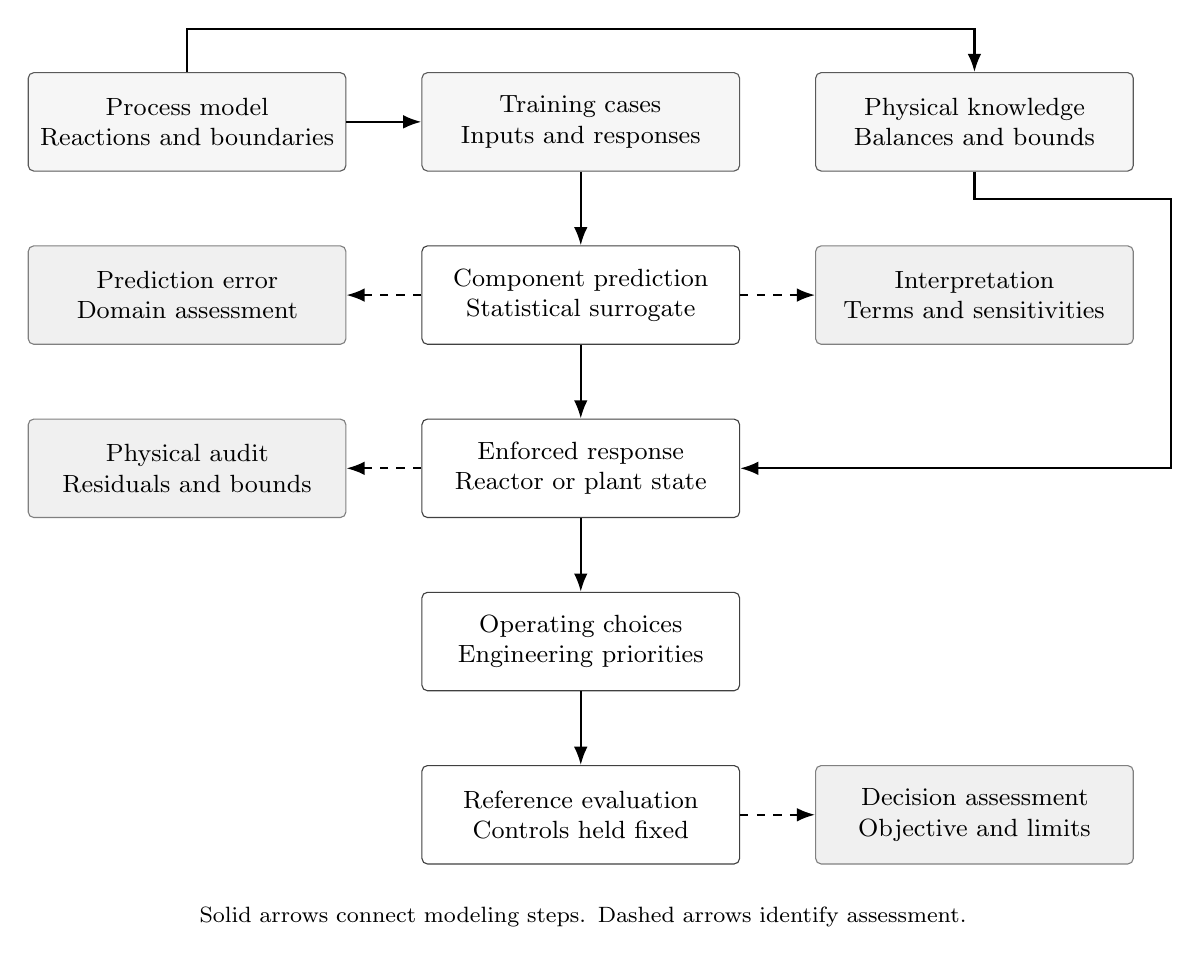
\begin{tikzpicture}[
  >=Latex,
  knowledge/.style={draw=black!65,rounded corners=2pt,fill=gray!7,
    text width=3.8cm,minimum height=1.25cm,align=center,font=\small},
  stage/.style={draw=black!75,rounded corners=2pt,fill=white,
    text width=3.8cm,minimum height=1.25cm,align=center,font=\small},
  evidence/.style={draw=black!50,rounded corners=2pt,fill=gray!12,
    text width=3.8cm,minimum height=1.25cm,align=center,font=\small},
  construction/.style={->,thick},
  assessment/.style={->,dashed,thick}
]
\node[knowledge] (mechanism) at (0,0)
  {Process model\\Reactions and boundaries};
\node[knowledge] (data) at (5.0,0)
  {Training cases\\Inputs and responses};
\node[knowledge] (physics) at (10.0,0)
  {Physical knowledge\\Balances and bounds};
\node[stage] (prediction) at (5.0,-2.2)
  {Component prediction\\Statistical surrogate};
\node[evidence] (accuracy) at (0,-2.2)
  {Prediction error\\Domain assessment};
\node[evidence] (inspection) at (10.0,-2.2)
  {Interpretation\\Terms and sensitivities};
\node[stage] (enforced) at (5.0,-4.4)
  {Enforced response\\Reactor or plant state};
\node[evidence] (audit) at (0,-4.4)
  {Physical audit\\Residuals and bounds};
\node[stage] (choice) at (5.0,-6.6)
  {Operating choices\\Engineering priorities};
\node[stage] (reference) at (5.0,-8.8)
  {Reference evaluation\\Controls held fixed};
\node[evidence] (decision) at (10.0,-8.8)
  {Decision assessment\\Objective and limits};
\draw[construction] (mechanism)--(data);
\draw[construction] (mechanism.north)--++(0,0.55)-|(physics.north);
\draw[construction] (data)--(prediction);
\draw[construction] (prediction)--(enforced);
\draw[construction] (physics.south)--++(0,-0.35)--++(2.5,0)
  |- (enforced.east);
\draw[assessment] (prediction)--(accuracy);
\draw[assessment] (prediction)--(inspection);
\draw[assessment] (enforced)--(audit);
\draw[construction] (enforced)--(choice);
\draw[construction] (choice)--(reference);
\draw[assessment] (reference)--(decision);
\node[align=center,text width=13.5cm,font=\footnotesize] at (5,-10.1)
  {Solid arrows connect modeling steps. Dashed arrows identify assessment.};
\end{tikzpicture}
\endgroup

\caption{Conceptual research logic linking process knowledge, component prediction, projection, interpretation, and independent assessment of operating choices.}
\label{fig:research_conceptual_logic}
\end{figure}

The mechanistic component concentrations serve as supervised targets paired with known influent and operating inputs. Predicted ammonium, substrate, biomass, and other concentrations are compared with these targets to assess error, while separate checks assess mass conservation, non-negativity, and the additional plant constraints. Structural inspection examines the fitted treatment relationships, and decision assessment evaluates the mechanistic response at the selected controls. Both the reactor and connected plant follow this logic, with their predictors and physical boundaries specified separately.

\section{Scope and limitations}

The study evaluates simulated steady-state responses of a standalone activated sludge reactor and a connected plant with biological reactors, secondary clarification, and recycle streams. Reference responses come from mechanistic equations with fixed process definitions and parameter values. The reactor and plant assessments each use a separately specified operating domain, so their findings are interpreted within the conditions examined.

The represented state contains organic, nitrogen, phosphorus, oxygen, alkalinity, biomass, and solids coordinates on the adopted model basis. Mass conservation is imposed within that basis and the stated system boundary, and non-negativity applies to the represented concentrations. These requirements define the extent of the physical guarantee. They do not establish complete elemental accounting for unrepresented species, full kinetic feasibility of every projected state, or dynamic stability beyond the specified checks \citep{TakacsVanrolleghem2006,Selerio2026}.

Predictive agreement in this study is agreement with the selected mechanistic reference under simulated conditions. Establishing performance at an operating treatment plant would require field evidence addressing calibration uncertainty, measurement error, microbial adaptation, and unrepresented reactions \citep{Machado2014,Newhart2019}. Reliable calibration and process understanding therefore remain essential for any practical extension of the framework \citep{Petersen2003,Meijer2004}.

Exploratory simulation informed the design of the connected plant assessment, so its reserved holdout cases provide descriptive evidence conditional on those design choices. This is termed post-selection assessment. Although fitting and tuning exclude the holdout responses, that separation does not make the assessment an independent external confirmation. Mechanistic evaluation supplies a reference check at the selected controls, while the statistical limitation associated with the assessment design remains.

Attached-growth treatment, spatial transport, resource-recovery networks, and dynamic control inform the background and possible extensions of the work, but are outside the evaluated case studies. The connected operating problem is confined to the declared plant topology and local numerical assessment. Its findings consequently do not certify a global optimum or establish a new network configuration.

Numerical examples and conceptual figures are explicitly hypothetical and explain the mathematical operations. Empirical treatment, prediction, optimization, and timing findings are presented separately in the reactor projection, structured-regression, and connected-plant assessments.
\chapter{Review of Related Literature}
\label{ch:literature}

Activated sludge surrogate modeling draws on several bodies of research that address different parts of the same engineering problem. Mechanistic models define the treatment processes, component transformations, and material balances that a surrogate must approximate. Data-driven studies show how treatment quantities can be estimated from measurements or simulations. Physical enforcement methods constrain predictions to satisfy specified balances and concentration bounds. Interpretable modeling provides ways to examine the fitted relationships, while optimization studies determine whether those predictions can support useful operating decisions. This chapter reviews these contributions as a connected body of work and identifies the questions that remain when they are brought together for complete-component activated sludge analysis.

\section{Mechanistic foundations of activated sludge modeling}

\subsection{Development of component and nutrient models}

Activated sludge modeling developed from the need to relate operating conditions to organic matter removal, oxygen demand, biomass growth, and sludge production. Early formulations established the basic connection between biological transformation and material accounting. \citet{Marais1976} formulated steady-state activated sludge analysis around substrate utilization and biomass, while \citet{Dold1981} developed a more general model that linked several biological processes within a common treatment calculation. Together, these contributions established the basis for calculating treatment responses from material balances and biological rates rather than treating effluent quality as an isolated empirical outcome.

This framework was expanded as activated sludge models became more component-resolved. \citet{Henze1987} presented the single-sludge framework associated with Activated Sludge Model No.\ 1 (ASM1), which distinguishes substrate, biomass, and nitrogen components so that carbon oxidation, nitrification, and denitrification can be calculated together. Later models addressed processes that this formulation did not represent explicitly. \citet{Henze1999} extended phosphorus-removal modeling to include the denitrifying activity of phosphorus-accumulating organisms, while \citet{Gujer1999} introduced Activated Sludge Model No.\ 3 (ASM3), which represents organic substrate storage and uses endogenous respiration to describe biomass decay.

These developments addressed different biological modeling needs. The phosphorus-removal extension connects nitrate use with phosphate behavior, while the storage-based formulation separates substrate uptake from its later use by biomass. The collected formulations in \citet{Henze2006} provide a common reference for these component definitions and their associated reaction terms. For surrogate modeling, their importance lies in defining what must be predicted. Effluent COD or TN can summarize treatment quality, but the underlying component concentrations describe the material forms that produce those totals. A surrogate intended to preserve process accounting therefore requires more than agreement with a small set of aggregate indicators.

The comparison of seven activated sludge models by \citet{Hauduc2013} further shows why the mechanistic reference must be specified before statistical models are compared. Their review examined how the models represent hydrolysis, fermentation, microbial growth and decay, and biological storage. The differences were not merely mathematical; they reflected different assumptions about treatment processes and available process knowledge. Model selection therefore depends on the treatment system and the question being studied. For a surrogate comparison, this means that all candidate predictors must approximate the same selected process model. Otherwise, differences in prediction may reflect different biological assumptions rather than differences among statistical learners.

\subsection{Biological dependence and calibration uncertainty}

The mechanistic literature also shows why operating conditions and influent composition cannot be interpreted independently. Nutrient-removal processes depend on the material entering the system and on how operating choices alter the conditions under which microorganisms compete and react. \citet{Wentzel1992} examined interactions among nitrification, denitrification, and excess phosphorus removal. \citet{Guerrero2011} studied competition for organic substrate in a pilot system designed for simultaneous nitrogen and phosphorus removal and found that the supplied carbon source affected the ability to maintain phosphorus removal when nitrate entered the initially anaerobic zone. Their results illustrate a specific biological dependence among substrate composition, recycle conditions, and nutrient removal.

For statistical modeling, these findings support retaining both operating conditions and component-resolved influent information. A model based only on total organic loading can overlook differences among carbon sources that perform different biological roles. Likewise, a model that treats aeration or recycle independently of loading can miss the conditions under which those operating changes influence nutrient removal. This provides a process-based reason to examine interaction terms in a treatment surrogate. It does not, however, imply that a fitted interaction coefficient identifies a microbial mechanism by itself. The statistical relationship and the biological mechanism remain distinct forms of evidence.

Calibration research addresses a related problem: even a mechanistically detailed model requires evidence that its parameters and internal quantities represent the treatment system of interest. \citet{Petersen2003} reviewed experimental designs for estimating activated sludge parameters, while \citet{Vanrolleghem1999} examined the use of respirometry, which measures oxygen consumption, to estimate model parameters and component combinations. These methods show that the information supplied by an experiment must correspond to the parameter or internal quantity being estimated.

The full-scale calibration study of \citet{Machado2014} makes this issue more explicit. They calibrated a phosphorus-removal model using data from a treatment plant in Manresa, Spain, assessed parameter confidence intervals, and examined how influent and operating variables affected the model fit. They also varied these inputs while retaining default kinetic and stoichiometric parameters to evaluate output sensitivity. Their analysis therefore considered uncertainty in both process inputs and biological parameters. For surrogate modeling, this distinction is important because simulated training targets inherit the assumptions of the mechanistic model that generates them. Agreement with those targets establishes how well the surrogate approximates that reference. Agreement with an operating treatment plant requires the additional evidence supplied by calibration and measurement.

The mechanistic literature therefore establishes the component definitions, reaction relationships, and calibration practices needed to give a surrogate prediction physical meaning. The unresolved question for this dissertation is not how to replace that mechanistic foundation, but how to approximate its defined treatment responses efficiently while retaining their material accounting. The surrogate is evaluated against an adopted mechanistic reference; calibration of that reference to a particular operating plant remains a separate task.

\subsection{Clarification and connected plant balances}

Biological reactors alone do not determine the final treatment response. The material leaving the reactor is subsequently separated, recycled, wasted, or discharged, so clarification and solids storage become part of the plant-level material account. \citet{Takacs1991} developed a clarification and thickening model based on solids fluxes and balances across layers of a one-dimensional settler. The model calculates solids profiles and overflow and underflow concentrations under steady and changing conditions. \citet{HartelPopel1992} likewise modeled secondary clarification with sludge thickening. These studies provide mechanistic descriptions of how suspended material is retained, concentrated, recycled, and discharged.

The difficulty of connecting biological and clarification models was examined directly by \citet{JeppssonDiehl1996}. They studied how biological components propagate through a secondary clarifier and identified problems that arise because the biological reactor and settler models represent particulate material differently. Their evaluation of component-transport algorithms focused particularly on the composition of sludge returned to the reactor. This result is important for surrogate modeling because it shows that predicting aggregate solids alone is not sufficient when the recycled stream must retain a biologically meaningful component composition.

\citet{Alex2008} addressed the broader need for comparable whole-plant assessment through Benchmark Simulation Model No.\ 1. The benchmark connects five biological compartments, a secondary settler, internal recycle, return sludge, and wasting, and specifies influent conditions, control settings, and assessment criteria. Its contribution is not only a plant configuration but a common setting in which alternative operating strategies can be compared. It makes explicit that biological conversion, solids separation, recirculation, and wasting form one connected treatment response.

Together, these studies define the relationships that a connected surrogate must preserve. A clarifier prediction affects both the discharged effluent and the recycled biomass returned to the biological tanks. Stored solids contribute to the inventory used in solids-retention calculations. Shared streams carry material from one unit to another and must therefore agree across unit boundaries. A single-reactor surrogate captures only part of this system. Extending physical enforcement to the plant level requires consistent component flows at these connections together with an explicit account of retained solids.

\section{Data-driven prediction of wastewater treatment responses}

\subsection{Soft sensors and reported treatment quantities}

Data-driven wastewater treatment research developed partly because operating plants collect large sets of measurements that are difficult to interpret jointly and because some important treatment quantities are costly, delayed, or difficult to measure directly. \citet{Newhart2019} reviewed methods for fault detection, variable prediction, and advanced process control and identified missing observations, outliers, correlated variables, and changing process behavior as recurring features of plant data. \citet{Sundui2021} reviewed machine learning applications across biological wastewater treatment. Together, these reviews establish a range of useful prediction tasks and emphasize that the choice of method depends on both the available information and the intended application.

Soft sensors are one example. A soft sensor estimates a quantity that is difficult or slow to measure from other observations that are easier to obtain. \citet{Ching2022} developed a soft sensor for five-day biochemical oxygen demand using extreme gradient boosting (XGBoost). They evaluated influent and effluent estimates at two treatment plants and used supporting measurements selected from variables such as COD, solids, nutrients, and simpler sensor readings. The model covered a wide range of oxygen-demand values and could accommodate missing supporting observations. Its contribution is therefore practical and specific: it provides a faster estimate of an otherwise slow water-quality measurement.

A similar distinction appears in effluent nutrient prediction. \citet{Wang2025} compared a mechanistic activated sludge model with six machine learning models for effluent TN prediction using one year of high-resolution municipal plant data. The mechanistic model reproduced the direction of TN variation, while the learned models achieved greater predictive accuracy in the assessed dataset. Feature-attribution analysis was also used to identify influential inputs. This study shows that statistical models can improve a defined effluent-prediction task while still allowing the fitted response to be inspected.

Other data-driven studies address operational quantities beyond effluent quality. \citet{Ekinci2023} predicted waste-sludge production using 208 daily observations from an advanced biological treatment plant in Turkey. Their inputs included flow, polymer dosage, and the amounts of solids and pollutants removed. They compared learning methods and reported improved prediction after feature selection. This adds a solids-management target to the quality indicators considered elsewhere. At the same time, its use of measured removal quantities illustrates how the available inputs depend on the prediction task. A model used before a proposed operating condition has been evaluated would require inputs available at that earlier decision stage.

The common achievement of these studies is reliable estimation of selected treatment quantities from available plant information. Such predictions can support monitoring, diagnosis, and particular operating analyses. The requirement in this dissertation is broader. When the goal is to check mass conservation, non-negativity, and the distribution of material among biological forms, the complete modeled component state becomes the relevant prediction target. Accuracy for TN, oxygen demand, or sludge production supplies useful evidence for those particular quantities, but it does not establish the accuracy or physical consistency of every modeled component.

\subsection{Component estimation and simulation-based surrogates}

Component-estimation studies move closer to the information used by mechanistic activated sludge models. \citet{Wang2024} used a backpropagation neural network to estimate five COD-related component quantities from measured influent COD. They first characterized those components in an operating plant and then evaluated the neural estimates against the measurements. Their reported prediction accuracy exceeded 80\% for the five assessed components. The study addresses a practical difficulty in mechanistic modeling: repeated experimental fractionation of influent COD components is demanding, yet those fractions are needed as model inputs.

That contribution differs from predicting the effluent component state produced by treatment. Influent fractionation estimates how incoming organic material is distributed among model categories. An effluent surrogate instead estimates how a defined influent changes under specified biological and operating conditions. The two tasks can complement one another, but they have different targets and therefore require different evidence. The component estimates of \citet{Wang2024} improve characterization of the material entering the model; they do not by themselves establish the complete treatment mapping investigated in this dissertation.

Simulation-based surrogates address that mapping more directly. \citet{Fang2011} combined an extended activated sludge model with a support vector surrogate and a genetic optimization search for a full-scale nutrient-removal system. Mechanistic simulations supplied the input--output relationship learned by the surrogate. Their optimization indicated that anoxic volume and internal recycle could be reduced while retaining the specified discharge quality. The study is an early example of a workflow in which mechanistic simulation generates the training data, statistical learning accelerates response evaluation, and optimization uses the learned approximation to select operating conditions.

\citet{He2023} used a similar simulation-to-surrogate logic for greenhouse-gas emissions from papermaking wastewater treatment. They fitted a Kriging surrogate to steady-state process simulations and reported a coefficient of determination above 0.96. The surrogate then supported analysis and optimization of controllable treatment variables. This work addresses the computational cost of repeatedly evaluating an environmental objective. Its prediction target, however, is the emissions measure rather than the complete component state required for the material-balance assessment of this dissertation.

A closer precedent is provided by \citet{Selerio2026}, who addressed complete single-reactor component prediction using invariant-constrained second-order regression. The study used 10,000 simulated steady-state cases with 20 effluent components and compared the structured regression with nine statistical predictors. Its assessment included changes in training size, errors in reported water-quality quantities, and physical violation diagnostics. This establishes a direct component-level activated sludge comparison and provides the foundation for the physical-enforcement and interpretation questions developed later in this chapter.

Table~\ref{tab:rrl_prediction_evidence} summarizes this progression from monitoring selected indicators to approximating complete process responses. The distinction is not that one task is inherently better than another. Rather, each prediction target establishes a different kind of evidence. The table therefore identifies what additional information is needed when the objective shifts from estimating a reported quantity to evaluating a complete activated sludge component state.

\begin{table}[htbp]
\centering\footnotesize
\caption{Treatment prediction studies and the scope of their evidence.}
\label{tab:rrl_prediction_evidence}
\begin{tabular}{>{\raggedright\arraybackslash}p{0.24\linewidth}>{\raggedright\arraybackslash}p{0.33\linewidth}>{\raggedright\arraybackslash}p{0.31\linewidth}}
\toprule Study and task & Contribution established & Additional question for this dissertation\\\midrule
\citet{Ching2022}\newline Oxygen-demand soft sensing & Estimation across two plants with support for missing sensor observations. & Can a predictor estimate the complete effluent state from influent and proposed operating inputs?\\
\citet{Wang2025}\newline Effluent TN prediction & Comparison of six learned models with a mechanistic model and inspection of influential inputs. & Are the individual nitrogen and other component concentrations accurate and physically consistent?\\
\citet{Wang2024}\newline Influent component estimation & Neural estimation of five COD-related quantities used in process modeling. & How accurately is the resulting effluent component state predicted after treatment?\\
\citet{Fang2011}\newline Simulation-based operating search & Mechanistic simulation combined with a support vector surrogate and optimization. & Can connected component predictions be constrained and checked at the selected controls?\\
\citet{Selerio2026}\newline Complete reactor prediction & Structured prediction of 20 components with physical checks and training-size assessment. & How do common projection and plant connections affect prediction and operating assessment?\\
\bottomrule
\end{tabular}
\end{table}

\subsection{Model comparison, data availability, and extrapolation}

The wastewater applications reviewed above use statistical learners with different assumptions about how nonlinear input--output relationships should be represented. Random forests, developed by \citet{Breiman2001}, average predictions from randomized decision trees. \citet{ChenGuestrin2016} developed XGBoost, while \citet{Ke2017} introduced the light gradient boosting machine (LightGBM). \citet{SmolaScholkopf2004} described support vector regression, which combines regularized fitting with kernel-based similarity. These methodological studies provide the statistical basis for several learners now used in wastewater treatment. Their differences justify comparing multiple model families rather than assuming that one fitting structure is best for every treatment response.

Inspectable linear and nonlinear models provide another part of that comparison. \citet{Wold2001} described partial least squares regression, which represents related variation in inputs and outputs through latent components. These latent statistical components are weighted combinations of variables and should not be confused with physical wastewater constituents. \citet{Woo2009} applied a kernel extension of partial least squares to estimate COD, TN, and cyanide concentrations in industrial cokes wastewater treatment. The nonlinear extension outperformed the assessed linear and other nonlinear partial least squares formulations in that application. This supports the value of nonlinear structure for the studied response while leaving ordinary partial least squares as a distinct baseline for other comparison tasks.

Broader tabular-learning research reinforces the value of comparing model families. \citet{ShwartzZiv2022} examined tabular machine learning, while \citet{Borisov2024} surveyed neural approaches for tabular data. Activated sludge surrogate inputs have a similar tabular form, with each case containing operating settings and influent concentrations. However, these methodological comparisons cannot determine the preferred learner for a specific treatment problem. That ranking must come from a common treatment target, a common data design, and a common evaluation procedure. The general literature therefore guides comparator selection, while the activated sludge benchmark supplies the process-specific evidence.

The amount of available training data adds another dimension to the comparison. \citet{VieringLoog2023} reviewed learning curves and showed that their shapes depend on the learner, the dataset, and the prediction task. A learning curve relates model performance to the number of training observations and therefore provides evidence about data efficiency. \citet{Selerio2026} applied this type of assessment to activated sludge reactor surrogates. The result characterizes performance within the stated input range, but a broader comparison still needs to determine how complete-state error and physical adjustment change together when the number of simulated training cases becomes small.

Such comparisons also depend on strict separation between model development and assessment information. \citet{Kaufman2012} defined information leakage and described how information unavailable at the intended prediction time can inadvertently enter model construction. In wastewater applications, this distinction is particularly important because downstream measurements may be available for monitoring but not for predicting a proposed operating condition before the treatment response has occurred. Scaling, preprocessing, and model tuning must likewise exclude observations reserved for final assessment. These requirements determine what an error score means; they do not imply that downstream measurements are inappropriate in studies whose stated purpose is monitoring.

The remaining comparative question therefore combines three issues: learner choice, training support, and operating domain. Existing indicator and component studies demonstrate that useful prediction is possible within their assessed conditions. What is still needed here is a common complete-state comparison in which several learners use the same inputs, outputs, data partitions, and error definitions. That assessment must also distinguish interpolation within the sampled domain from prediction beyond it. Only then can component error and physical validity be evaluated together as influent and operating conditions change.

\section{Methods for imposing physical constraints on predictions}

\subsection{Physical guidance during fitting}

Machine learning models can reproduce observed responses while violating the equations or bounds that define a physically acceptable process state. A major branch of physics-informed learning addresses this problem by incorporating governing relations directly into model fitting. \citet{Karniadakis2021} reviewed approaches that combine physical knowledge with machine learning. One influential example is the residual-based formulation of \citet{Raissi2019}, in which discrepancies in governing differential equations are added to the training objective. Equation disagreement is therefore penalized alongside prediction error, allowing process knowledge to guide learning even when response observations are limited.

Wastewater applications provide direct evidence for this idea. \citet{Li2024} examined physics-informed neural models for water-treatment unit dynamics, including an activated sludge reactor. They compared physically informed models with conventional learned models under limited data and changing loading conditions. The physically informed models showed stronger predictive capability and generalization in the assessed systems. Their results demonstrate that governing equations can provide useful learning information when data alone are insufficient.

The distinction between physical guidance and physical enforcement is important, however. A finite residual penalty balances equation agreement against the other terms in the fitting objective. It can reduce violations without requiring every new prediction to satisfy the relevant equality exactly. The contribution of \citet{Li2024} therefore concerns improved learning through physical information. If the engineering requirement is that every returned component state satisfy mass conservation and concentration bounds, an additional output construction, projection, or numerical check is still required. Physical guidance during fitting and exact sample-specific enforcement address complementary questions.

\subsection{Conservation through model construction}

A second approach is to build conservation directly into the way model outputs are constructed. \citet{Beucler2021} introduced neural architectures that encode analytic constraints and compared them with constraints imposed through a loss function. In their climate-convection application, the architectural formulation enforced the selected conservation laws to machine precision without degrading overall predictive performance. Their results show that, when the output representation is designed appropriately, known equalities can be satisfied by construction rather than encouraged through a penalty.

Related work has used stoichiometric structure to couple predicted species. \citet{SturmWexler2020} developed a conservation framework in which learned transfers are converted into species changes through balanced process relationships. \citet{SturmWexler2022} later placed the stoichiometric mapping in a fixed neural layer for a photochemical surrogate. This construction avoided the need to reconstruct all reaction transfers as separate learning targets while retaining atom conservation in the predicted species changes. The common idea is that conservation is carried by the mapping between process changes and the final species response.

That idea transfers naturally to activated sludge modeling because stoichiometry also defines allowable combinations of component changes. However, conservation alone does not guarantee a physically acceptable concentration state. A balanced change can still consume more of a component than is available and thereby produce a negative concentration. The distinction follows from the difference between constraining a reaction-induced change and constraining the final state. The physical claim must therefore be matched to the quantity that the model construction actually restricts.

\citet{Harder2022} illustrated this broader requirement in an aerosol microphysics surrogate by examining both physical penalties and constrained output completion. Their assessment treated mass conservation and positive mass as separate but simultaneous concerns. The lesson for activated sludge prediction is direct: the complete returned state must be assessed for both balance satisfaction and concentration bounds after every stage of prediction has been applied.

\subsection{Projection after statistical prediction}

Projection provides another route to physical enforcement. Instead of changing the fitted learner, a prediction is first produced and then adjusted to satisfy specified constraints. \citet{SturmSilva2024} developed a species-weighted least-squares correction for atom conservation in an atmospheric chemistry surrogate. Their weights accounted for the magnitude and uncertainty of individual species changes. In the reported assessment, an unweighted correction could damage prediction of a small radical, whereas weighting retained its accuracy and slightly improved overall agreement. The enforced conservation relation was unchanged; what changed was the way the required adjustment was distributed among species.

The same issue arises in activated sludge prediction because component concentrations can differ by several orders of magnitude. A correction that is numerically small relative to an abundant substrate may be large relative to a residual nutrient concentration. The results of \citet{SturmSilva2024} therefore motivate assessing projection size and component error together rather than treating physical correction as neutral with respect to prediction quality. Their method addresses an equality constraint, however, so an additional construction is needed when non-negativity must also be guaranteed.

\citet{KircherVotsmeier2025} addressed this joint requirement through a positivity-preserving projection followed by linear interpolation backtracking. They evaluated the method on atmospheric chemistry, heterogeneous catalysis, and synthetic reaction networks. The corrected predictions satisfied atom balances and remained positive in the tested systems without reducing overall prediction accuracy. This establishes a general procedure for imposing both conservation and positivity across different underlying surrogates. The remaining question for activated sludge analysis is how such a procedure behaves with wastewater component scales, reactor boundaries, limited training data, and inputs that move beyond the sampled domain.

A direct activated sludge example is provided by \citet{Selerio2026}. The structured regression in that study used physical penalties during fitting, then checked each raw prediction and projected it onto the mass conservation equalities. If non-negativity still failed, a linear program---an optimization problem with a linear objective and linear constraints---was used to complete the correction. The published assessment reported no final mass conservation or non-negativity violations. Because the raw regression itself did not satisfy both requirements, the final enforcement procedure was the stage responsible for the physical guarantee.

That result also illustrates why physical validity and predictive accuracy must be evaluated separately. The structured surrogate was not the most accurate method under every reported score, even though its final states satisfied the declared constraints. Physical enforcement therefore establishes that the returned state belongs to the specified feasible set; it does not establish that the state is the closest possible approximation to the mechanistic reference. The next comparative question is consequently a paired one: when the same raw predictions are held fixed, how does projection change error, adjustment size, and computational cost across several activated sludge learners?

Figure~\ref{fig:rrl_enforcement_locations} places the reviewed methods along the prediction pipeline. Fitting penalties guide learning toward equation agreement, constrained output constructions impose selected relations through the model architecture, and final-state projection corrects the prediction after it has been produced. These approaches can all introduce physical information, but they make different guarantees because they act at different stages.

\begin{figure}[htbp]
\centering
\begingroup\linespread{1}\selectfont
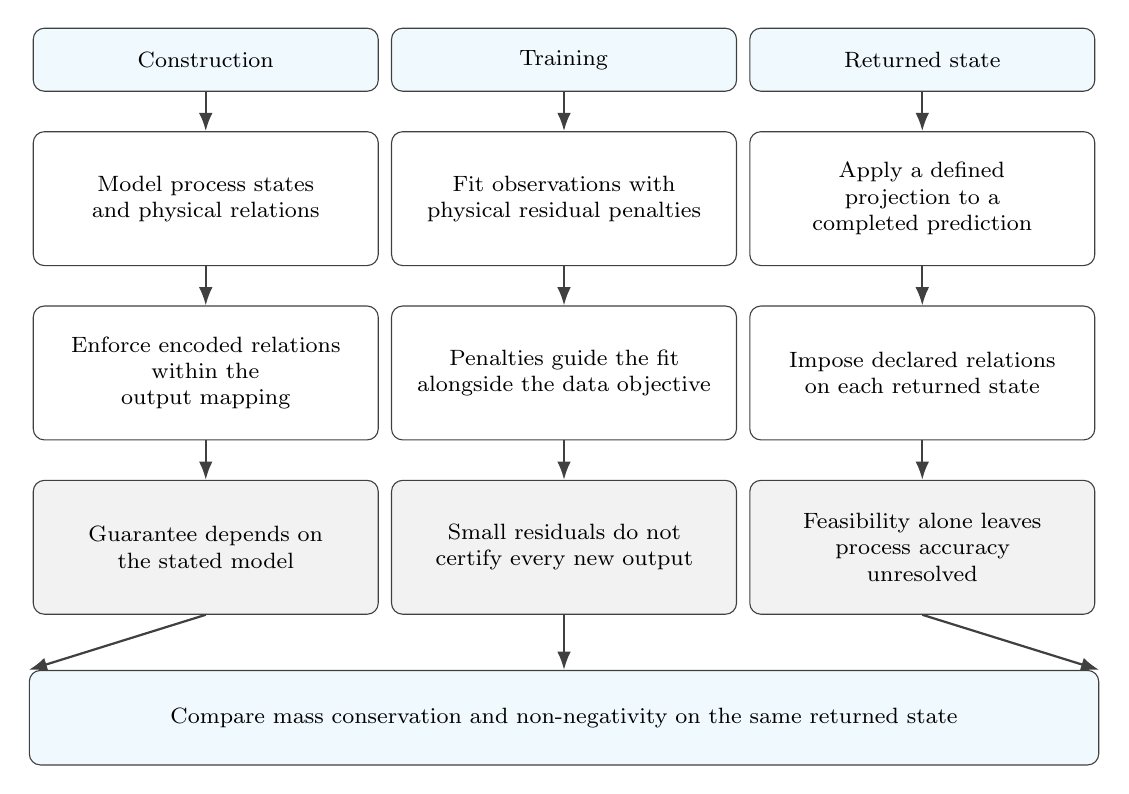
\begin{tikzpicture}[>=Latex,node distance=5mm,
heading/.style={draw=black!75,rounded corners,fill=cyan!6,text width=4.1cm,minimum height=8mm,align=center,font=\footnotesize,inner sep=4pt},
block/.style={heading,fill=white,minimum height=17mm},
limit/.style={block,fill=black!5},
flow/.style={->,thick,draw=black!75}]
\node[heading] (lh) at (-4.55,0) {Construction};
\node[heading] (mh) at (0,0) {Training};
\node[heading] (rh) at (4.55,0) {Returned state};
\node[block,below=of lh] (l1) {Model process states\\and physical relations};
\node[block,below=of mh] (m1) {Fit observations with\\physical residual penalties};
\node[block,below=of rh] (r1) {Apply a defined\\projection to a\\completed prediction};
\node[block,below=of l1] (l2) {Enforce encoded relations\\within the\\output mapping};
\node[block,below=of m1] (m2) {Penalties guide the fit\\alongside the data objective};
\node[block,below=of r1] (r2) {Impose declared relations\\on each returned state};
\node[limit,below=of l2] (l3) {Guarantee depends on\\the stated model};
\node[limit,below=of m2] (m3) {Small residuals do not\\certify every new output};
\node[limit,below=of r2] (r3) {Feasibility alone leaves\\process accuracy\\unresolved};
\node[heading,text width=13.3cm,minimum height=12mm,below=7mm of m3] (common)
{Compare mass conservation and non-negativity on the same returned state};
\draw[flow] (lh)--(l1); \draw[flow] (l1)--(l2); \draw[flow] (l2)--(l3);
\draw[flow] (mh)--(m1); \draw[flow] (m1)--(m2); \draw[flow] (m2)--(m3);
\draw[flow] (rh)--(r1); \draw[flow] (r1)--(r2); \draw[flow] (r2)--(r3);
\draw[flow] (l3.south)--(common.north west);
\draw[flow] (m3.south)--(common.north);
\draw[flow] (r3.south)--(common.north east);
\end{tikzpicture}

\endgroup
\caption{Stages at which the reviewed methods introduce physical information. Fitting penalties guide equation agreement. Output construction and projection impose the relations encoded in their formulations. Simultaneous mass conservation and non-negativity require an assessment of the final component state.}
\label{fig:rrl_enforcement_locations}
\end{figure}

\subsection{Constraint scope and recent extensions}

Recent work has expanded constrained learning beyond deterministic point predictions. \citet{Hansen2024} used integral conservation relations to adjust probabilistic predictions while accounting for both predicted means and uncertainty. Their framework enforced conservation exactly when the imposed balance was assigned zero uncertainty and was evaluated on a family of transport equations. \citet{Utkarsh2025} trained a probabilistic predictor together with a differentiable projection and evaluated the approach on differential-equation and time-series problems. Because the projection is differentiable, its effect can participate directly in gradient-based learning. These studies extend physical enforcement from correcting one predicted state to representing uncertainty within the constrained prediction process.

Other work has examined the expressive capacity of hard-constrained models. \citet{Min2024} developed neural output layers for input-dependent linear and convex constraints and established approximation results under the stated mathematical conditions. A convex feasible set contains the straight line joining any two feasible states, which permits useful mathematical guarantees for constrained outputs. \citet{Valente2025} examined projection onto physical manifolds, or sets of outputs satisfying selected physical laws, using spring-mass and reactive-plasma examples. Their work extends correction beyond simple linear relations to nonlinear physical structures.

These contributions broaden the available tools for physically constrained machine learning, but they do not remove the need to define the wastewater-specific constraint set carefully. The literature already provides methods for enforcing conservation and, in some cases, conservation together with positivity. The gap addressed in this dissertation is therefore not the absence of physical enforcement methods. It is the need to determine how common enforcement affects accuracy, adjustment size, and computational cost for a complete activated sludge component response and then to extend the material-accounting requirements from a single reactor to a connected plant. The imposed constraints remain intentionally narrower than the complete biological and settling equations.

\section{Interpretable modeling of treatment responses}

\subsection{Inspection of inputs and fitted relationships}

Interpretability concerns what can be learned about a model's response after it has been fitted. \citet{Rudin2019} argued for using directly inspectable models in consequential applications when suitable interpretable alternatives are available. In wastewater treatment, this becomes relevant when an engineer needs to understand how influent composition, aeration, recycle, or another operating variable contributes to a predicted treatment outcome. The argument supports examining the model that informs the decision. It does not imply that every visible statistical coefficient has a direct biological interpretation.

Several treatment studies use post-fitting inspection to identify influential variables. \citet{Wang2025} combined effluent TN prediction with feature-attribution analysis, while \citet{Ekinci2023} used feature selection and attribution in sludge prediction. These approaches help identify which observed variables contribute to a particular statistical output and can guide process investigation or reduce unnecessary inputs. Their explanations, however, apply to the fitted TN or sludge model. They do not describe how every component in a mechanistic activated sludge state responds.

Explicit algebraic models provide a complementary form of interpretability. \citet{Nazlabadi2021} reviewed response-surface methods in biological wastewater treatment, where polynomial terms describe operating effects and interactions over a fitted domain. \citet{Brunton2016} developed sparse equation discovery from candidate functions for nonlinear dynamical systems. The latter provides a methodological precedent for inspecting named terms, while response-surface applications provide a direct wastewater-treatment context. Together, they show why visible mathematical structure can be useful when the objective is to understand how inputs contribute to a predicted response.

For activated sludge analysis, the distinction among terms matters. An aeration term represents a fitted dependence on aeration, an influent substrate term represents a fitted dependence on loading, and their product allows the aeration response to change with the substrate condition. Such terms can make the statistical response easier to examine within the fitted domain. They do not, by themselves, establish causal biological parameters. Demonstrating a microbial mechanism would require a different identification problem and different evidence, particularly when the model inputs are correlated.

\subsection{Structured regression and the final projected state}

\citet{Selerio2026} addressed the need for an inspectable complete-component activated sludge surrogate by separating operating effects, influent effects, curvature, interactions, and learned dependence among effluent components. The explicit second-order terms allow the fitted input relationships to be examined in physical coordinates. Component coupling then contributes to the complete raw state, and a fixed composition map converts that state into reported water-quality quantities. The result is a treatment surrogate whose statistical structure can be traced from inputs to component predictions and then to aggregate treatment indicators.

The same study also shows why interpretability cannot stop at the fitted coefficients when the deployed prediction includes physical correction. Its displayed coefficient relationships describe the raw regression before final constraint enforcement. Mass conservation projection and the subsequent linear-program stage can change the concentrations ultimately returned to the engineer. If a concentration bound becomes active, the local sensitivity of the final prediction can also differ from the slope implied by the unconstrained equation. The study therefore distinguishes the displayed raw coefficient structure from derivatives of the final projected response.

This distinction becomes especially important when component coupling is present. A visible coefficient can affect one intermediate quantity, which then influences several components through the coupling relation before projection imposes the physical constraints. Different fitted coefficient combinations can also produce similar predictions. \citet{Selerio2026} therefore identifies coefficient stability across resampled training data as an additional diagnostic rather than assuming that one fitted coefficient set uniquely represents the treatment process.

The broader literature on differentiable hybrid modeling supports this complete-response perspective. \citet{Shen2023} reviewed approaches that connect learned relationships with process equations and showed, through geoscience examples, how combined models can retain physical knowledge while remaining open to interpretation. They also identify verification of the physical significance of outputs as an ongoing need. For the present dissertation, this supports following the prediction through all of its stages rather than interpreting only the first fitted equation.

The remaining interpretive question is therefore an extension of an established contribution. The raw structured regression already exposes its terms. What remains is to connect those terms to component coupling, reporting, and the constraints that determine the final effluent response, and to examine how stable the inferred relationships remain as training cases change. This preserves the distinction between statistical association and biological mechanism while making the complete deployed calculation available for engineering interpretation.

\section{Surrogate modeling for operating decisions}

\subsection{Mechanistic and learned routes to operating optimization}

Optimization of activated sludge operation predates the recent use of machine learning surrogates. Mechanistic studies established how treatment constraints, influent conditions, and operating degrees of freedom can be brought into one decision problem. \citet{Araujo2013} optimized a steady-state process model and used sensitivity analysis to identify variables for economic control. Their analysis linked active effluent constraints and remaining operating degrees of freedom to the resulting control structure. \citet{Nazif2023} calibrated a treatment model to a plant in Tehran, grouped influents according to quantitative and qualitative characteristics, and optimized operating settings for each group. These studies provide examples of direct process-based optimization in which operating decisions are evaluated through the mechanistic treatment model itself.

Learned surrogates provide an alternative when repeated mechanistic calculations are expensive. \citet{Fang2011} trained a support vector surrogate on mechanistic simulations and then used the learned model in an optimization of a nutrient-removal system. \citet{KusiakWei2013} fitted neural models for airflow, effluent carbonaceous biochemical oxygen demand, and TSS from industrial data and used a multiobjective particle-swarm search to examine dissolved-oxygen settings. These studies demonstrate that a learned treatment response can be used directly in the search for operating conditions. The engineering meaning of the result, however, depends on the particular outputs that the surrogate predicts and on how those outputs represent the objectives and constraints of the decision.

Dynamic control studies provide related evidence at a different time scale. \citet{Bernardelli2020} developed a neuro-fuzzy predictive controller for aeration and field-tested it at a large municipal plant, reporting improved effluent quality and energy savings in that application. \citet{Croll2023} reviewed reinforcement learning for wastewater control and discussed the methods and challenges involved in changing operation over time. These contributions show that learned models can participate directly in treatment control. The present dissertation addresses a different question: fixed-input steady-state operating assessment. Dynamic control results therefore provide important context without replacing the need for a separate evaluation of the steady-state decision problem.

The operating literature establishes that both mechanistic and learned routes can be used to select treatment settings. The unresolved question for a new surrogate is whether its selected settings remain favorable when both routes are judged on the same engineering basis. Such a comparison requires common treatment objectives, operating bounds, and reference calculations. It also requires separating the one-time cost of developing a surrogate from the computational cost of repeatedly using it during an operating search.

\subsection{Integrated resource recovery and connected responses}

Whole-system wastewater studies broaden the decision beyond the performance of a single biological reactor. \citet{PadronPaez2020} examined sustainable treatment design through multiple objectives, while \citet{Aboagye2021} combined wastewater-network design, optimization, and sustainability assessment. Their work shows how treatment quality and resource priorities can be considered together when several process choices are available. This provides the broader systems context for a connected plant objective in which treatment gains must be considered alongside the resources required to obtain them.

\citet{Durkin2024} extended this idea through surrogate-based process synthesis for resource recovery from brewery wastewater. Their framework combined high-fidelity simulations, regression surrogates, and classification models for process feasibility. The application considered biogas recovery, recoverable nutrient quality, aeration demand, and uncertainty in wastewater composition. It therefore demonstrates that learned approximations can support integrated decisions involving several resource pathways while accounting explicitly for whether a simulated configuration is feasible.

The decision problem in this dissertation is related but different. \citet{Durkin2024} considered a network-design problem with alternative process configurations. The present connected operating study retains a specified activated sludge topology and predicts the mixer, biological reactor stages, clarifier outlets, and stored solids jointly. Its additional requirement is that those predicted quantities remain mutually consistent at the fixed physical connections of the plant. A classifier indicating simulator feasibility and an explicitly imposed component balance therefore address different aspects of model reliability.

The single-reactor work of \citet{Selerio2026} supplies a precedent for physical enforcement at one biological unit, while the benchmark of \citet{Alex2008} provides a mechanistic precedent for comparing connected plant responses and controls. Bringing these lines of research together leads to a specific remaining question: can a statistical plant response preserve the declared unit connections and solids inventories while still supporting useful operating decisions? Answering that question requires evidence beyond single-reactor feasibility and beyond the accuracy of one aggregate operating objective.

\subsection{Approximation error at selected operating conditions}

A surrogate can have good average predictive accuracy and still be inaccurate where the optimizer ultimately chooses to operate. Surrogate-optimization research addresses this distinction directly. \citet{BhosekarIerapetritou2018} reviewed surrogate modeling for feasibility analysis and optimization, while \citet{McBride2019} reviewed surrogate construction from experiments and simulations for process-system decisions. Both place prediction within a larger decision workflow: the surrogate must approximate the quantities and the operating region that matter to the optimization, not merely reproduce an average response over the original training design.

\citet{Alexandrov1998} developed a trust-region framework that manages approximation models during optimization by using reference information to assess local model quality and control the region in which the approximation is trusted. The contribution is methodological, but its implication for wastewater treatment is clear. A model used to select aeration, recycle, or wasting settings should be checked near the controls that the optimizer actually selects rather than judged only by an average error calculated elsewhere in the operating domain.

The distinction between predictive quality and optimization quality was examined explicitly by \citet{Pedrozo2025}. They compared five surrogate approaches for a carbon-dioxide-stream pooling problem and assessed predictive accuracy, computational effort, and optimization behavior separately. Their comparison of one-shot optimization with a trust-region filter strategy showed that models with favorable fitting performance could still differ in convergence and reliability during search. Although the application concerns carbon capture rather than wastewater treatment, the methodological lesson is directly relevant: a good surrogate fit and a good engineering decision are separate outcomes.

Physical feasibility does not eliminate this distinction. Mass conservation and non-negativity remove certain impossible component states, but many different physically admissible states can still have different nitrogen distributions, biomass concentrations, and treatment performance. An optimizer can therefore select a prediction that satisfies the declared physical constraints yet remains inaccurate relative to the mechanistic reference. Physical-enforcement studies establish how to exclude impossible states; approximation-management studies establish why the response used by the optimizer still needs to be checked.

Together, these findings motivate independent mechanistic evaluation of the aeration, recycle, wasting, and other controls selected by the surrogate. The remaining decision gap concerns the complete body of evidence for a connected activated sludge surrogate. Its unit balances and stored solids must be mutually consistent. Its selected controls must satisfy the original treatment requirements when those controls are returned to the reference model. Its objective must be evaluated on the same mechanistic basis as the direct comparator. Search time and verification effort must also be reported on a clearly defined basis. Only then can computational benefit and decision quality be assessed without assuming that physical constraint satisfaction establishes either one.

\section{Synthesis of established contributions and remaining gaps}

\subsection{What the reviewed studies have addressed}

The literature reviewed in this chapter shows a clear progression from process representation to engineering decision support. Mechanistic activated sludge models define components, biological reactions, separation, recirculation, and solids inventories. Calibration studies connect those model quantities to observations from real treatment systems. Data-driven soft sensors and indicator models improve estimation of selected treatment responses. Simulation-based surrogates extend learned prediction to repeated process calculations and optimization. Physics-informed and constrained-learning methods introduce governing relations into fitting or impose them on model outputs. Interpretable regression and surrogate-optimization research then address how fitted responses can be examined and how they should be evaluated when used to make operating decisions.

Several requirements relevant to this dissertation have therefore already been addressed in important forms. \citet{KircherVotsmeier2025} established joint atom balance and positivity for specified reactive-chemistry surrogates. \citet{Selerio2026} established final mass conservation and non-negativity for a structured activated sludge reactor surrogate and showed why interpretation must distinguish the raw and projected responses. \citet{Durkin2024} demonstrated surrogate-supported optimization for integrated wastewater resource recovery. These studies are not gaps that the dissertation claims to fill. They are the starting points from which its more specific questions arise.

The remaining gaps appear when these established contributions are brought into one complete-component activated sludge assessment. A comparison of learners must use the same component target. Physical enforcement must be evaluated not only for feasibility but also for the errors and adjustments it introduces. Interpretation must follow the prediction through coupling and projection rather than stopping at the visible regression terms. Plant-level decisions must preserve unit connections and then be checked on the original mechanistic basis. Table~\ref{tab:rrl_evidence_gap_matrix} summarizes this relationship between the established literature and the specific questions retained for the dissertation.

\begin{table}[htbp]
\centering\footnotesize
\caption{Established studies and the remaining questions addressed by the dissertation.}
\label{tab:rrl_evidence_gap_matrix}
\begin{tabular}{>{\raggedright\arraybackslash}p{0.22\linewidth}>{\raggedright\arraybackslash}p{0.34\linewidth}>{\raggedright\arraybackslash}p{0.32\linewidth}}
\toprule Research need & Studies addressing the need & Remaining question\\\midrule
Complete treatment prediction & \citet{Wang2025} assesses TN prediction. \citet{Wang2024} estimates influent components. \citet{Selerio2026} predicts complete reactor components. & How do several learners compare on one complete-state target under training scarcity and extrapolation?\\
Physical validity of predictions & \citet{Beucler2021} and \citet{SturmWexler2022} impose conservation. \citet{KircherVotsmeier2025} and \citet{Selerio2026} address conservation and concentration bounds together. & How does common enforcement affect component accuracy, adjustment size, and cost across learners?\\
Interpretation of treatment responses & \citet{Wang2025} inspects input contributions. \citet{Selerio2026} exposes regression terms and distinguishes raw from final interpretation. & How do coupling, reporting, and active constraints affect sensitivities and stability of the explanation?\\
Connected operating decisions & \citet{Fang2011} and \citet{Durkin2024} use surrogates in treatment decisions. \citet{Alex2008} defines a connected plant benchmark. & Can joint component enforcement support settings that remain credible under independent plant evaluation?\\
\bottomrule
\end{tabular}
\end{table}

\subsection{The four linked questions of the dissertation}

The first gap concerns comparative prediction of the complete reactor response. Existing indicator studies show that machine learning can predict useful treatment quantities, while the structured-regression study of \citet{Selerio2026} extends prediction to all modeled reactor components. What remains is a common comparison across learning families in which the target, partitions, and assessment scales are held fixed. That comparison must also show how performance changes as the number of training cases decreases and as influent or operating conditions move beyond the sampled domain. The purpose is not to identify one universally superior learner, but to determine how learner choice depends on the available data and the intended input range.

The second gap concerns what physical enforcement changes after a raw prediction has already been produced. Joint mass conservation and concentration bounds have been established by existing methods. The remaining question is how a common enforcement procedure affects the same raw predictions across several activated sludge learners. Component error, physical residuals, negative concentrations, projection displacement, and computational cost describe different consequences of that correction. Evaluating them together makes it possible to determine the value of enforcement without assuming that physical compliance must also improve predictive accuracy.

The third gap concerns interpretation of the complete returned treatment state. Structured regression already provides visible operating, loading, curvature, interaction, and coupling terms. However, the response ultimately used in engineering analysis can differ from the raw equation because coupling, reporting, and projection occur afterward. The remaining question is therefore how sensitivities pass through those stages, particularly when concentration bounds become active, and whether the resulting fitted relationships remain stable when the training cases change. This extends interpretation from the visible regression to the complete prediction actually returned to the engineer.

The fourth gap concerns connected prediction and operating assessment. Mechanistic plant models establish the shared streams, clarification behavior, recycle structure, and stored solids that connect treatment units. Surrogate studies establish that learned models can support operating and resource-recovery decisions. What remains here is to combine those requirements in one connected component response, impose the declared plant relations jointly, and then independently calculate treatment outcomes at the controls selected by the surrogate. Comparison with direct mechanistic optimization places both routes on the same treatment and resource basis and separates faster search from better decision quality.

Figure~\ref{fig:rrl_intersecting_gaps} shows why these four questions cannot be treated independently. The component concentrations being predicted are also the quantities adjusted by physical enforcement and examined during interpretation. Those same concentrations determine treatment indicators and enter the operating objective and constraints. A change introduced by projection can therefore affect component error, local sensitivity, and the settings selected during optimization. The integrated assessment must follow this shared treatment response through each stage rather than allowing evidence from one stage to stand in for another.

\begin{figure}[htbp]
\centering
\begingroup\linespread{1}\selectfont
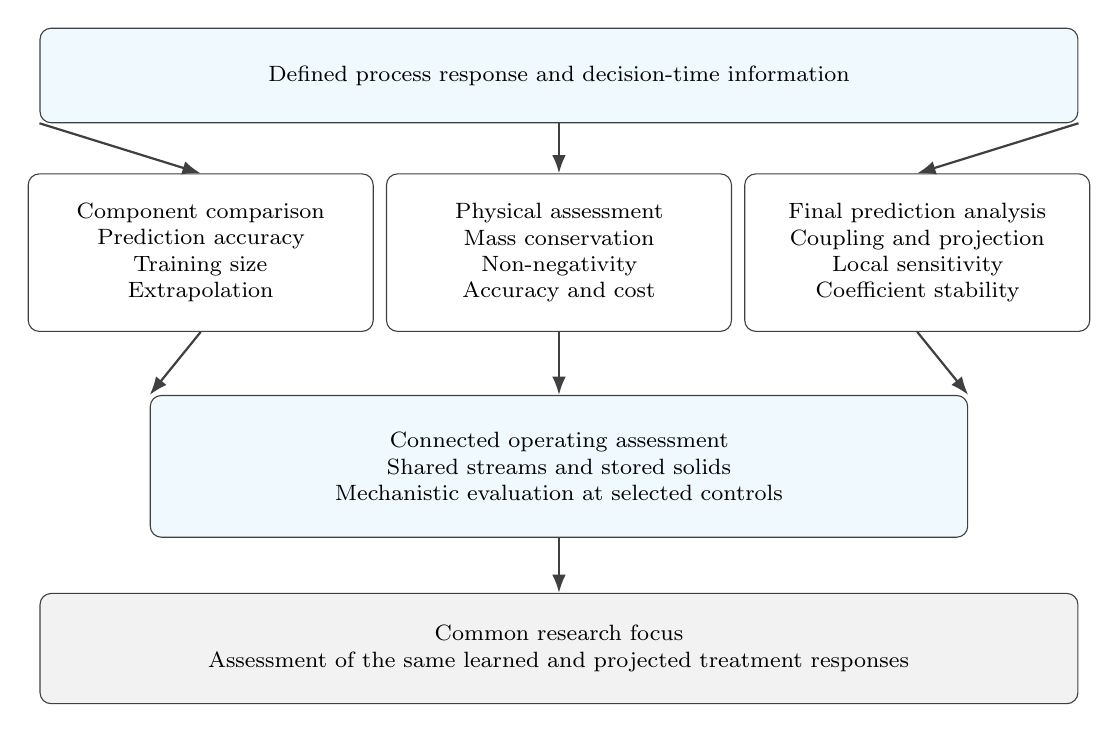
\begin{tikzpicture}[>=Latex,node distance=7mm,
block/.style={draw=black!75,rounded corners,fill=cyan!6,align=center,font=\footnotesize,inner sep=4pt},
evidence/.style={block,text width=4.1cm,minimum height=20mm,fill=white},
flow/.style={->,thick,draw=black!75}]
\node[block,text width=12.9cm,minimum height=12mm] (scope) at (0,0)
{Defined process response and decision-time information};
\node[evidence] (stat) at (-4.55,-2.25)
{Component comparison\\Prediction accuracy\\Training size\\Extrapolation};
\node[evidence] (phys) at (0,-2.25)
{Physical assessment\\Mass conservation\\Non-negativity\\Accuracy and cost};
\node[evidence] (interp) at (4.55,-2.25)
{Final prediction analysis\\Coupling and projection\\Local sensitivity\\Coefficient stability};
\node[block,text width=10.1cm,minimum height=18mm,below=8mm of phys] (decision)
{Connected operating assessment\\Shared streams and stored solids\\Mechanistic evaluation at selected controls};
\node[block,text width=12.9cm,minimum height=14mm,fill=black!5,below=7mm of decision] (gap)
{Common research focus\\Assessment of the same learned and projected treatment responses};
\draw[flow] (scope.south west)--(stat.north);
\draw[flow] (scope.south)--(phys.north);
\draw[flow] (scope.south east)--(interp.north);
\draw[flow] (stat.south)--(decision.north west);
\draw[flow] (phys.south)--(decision.north);
\draw[flow] (interp.south)--(decision.north east);
\draw[flow] (decision)--(gap);
\end{tikzpicture}

\endgroup
\caption{Links among the remaining comparative, physical, interpretive, and operating questions. Each question concerns the same defined activated sludge response. Established methods address parts of the problem, while their combined use requires common component and decision assessment.}
\label{fig:rrl_intersecting_gaps}
\end{figure}

The literature therefore supports a progression from a defined reactor response to a physically checked and independently evaluated plant decision. Chapter~\ref{ch:foundations} develops the common component and mechanistic basis for that progression. Chapter~\ref{ch:projection} compares reactor predictors and examines the effect of physical enforcement on the same raw responses. Chapter~\ref{ch:interpretable} develops the structured regression and follows interpretation through component coupling and projection. Chapter~\ref{ch:plant} extends the framework to a connected activated sludge plant and independently evaluates the controls selected through surrogate-assisted and direct mechanistic optimization. Chapters~\ref{ch:projection}--\ref{ch:plant} each present the rationale, theory, methodology, results, and discussion for their corresponding assessment, while Chapter~\ref{ch:conclusion} brings their findings together and identifies directions for future research.
\chapter{Mechanistic Foundations of Physically Admissible Prediction}
\label{ch:foundations}

\section{The component state as the object of prediction}

An activated sludge reactor does not simply remove material; it changes its form and distribution. Organic substrate can become biomass, ammonium can become nitrite and nitrate, and soluble phosphate can enter biological storage or a precipitate. Describing these transformations therefore requires more than a small set of aggregate effluent concentrations. The ASM framework addresses this need by separating wastewater material into components and linking their changes through biological and chemical processes \citep{Henze2006}. In this dissertation, that component representation also defines the physical meaning of a surrogate prediction: the surrogate estimates a complete component state from the influent state and operating conditions.

The mechanistic reference is Activated Sludge Model No.\ 2d with two-step nitrification (ASM2d-TSN). It combines the phosphorus-removal framework of \citet{Henze2006} with the nitrogen-transformation formulation used by \citet{Guerrero2011}. The model contains 20 components and 28 processes, with ten dissolved and ten particulate components. Stoichiometry specifies the relative amounts of material consumed and produced by each process, while kinetics specifies how rapidly those processes proceed as functions of the reactor state and fixed parameters. The surrogate approximates the resulting steady-state concentrations. Projection then imposes selected physical accounting constraints on those predictions.

This chapter develops the mechanistic basis for that procedure. It first defines how the component state is represented and manipulated mathematically, then connects the components to the biological transformations of the activated sludge model. It subsequently derives the reactor balances, the mass conservation invariants used for physical enforcement, the geometry of physically admissible states, and the reporting map from component concentrations to familiar water quality quantities. These ideas provide the common foundation for the surrogate models and optimization studies developed in Chapters~\ref{ch:projection}--\ref{ch:plant}.

\subsection{Reading component vectors and matrix operations}

The component formulation uses vectors and matrices to record many concentration and balance equations at once. Their meaning remains scalar, however: each coordinate still represents one physical quantity with a specified unit. For example, a concentration of 5 g N m$^{-3}$ is numerically equal to 5 mg N L$^{-1}$ because both the mass and volume units change by a factor of one thousand. Oxygen, COD, nitrogen, phosphorus, solids, and alkalinity nevertheless use different reporting bases. A quantity expressed as g COD m$^{-3}$, for instance, represents oxygen-demand equivalents rather than grams of one named organic molecule. These distinctions determine which coefficients are needed before quantities can be combined.

A vector collects related scalar values in a fixed order. A three-component column vector and its transpose can be written as
\[
c=\begin{bmatrix}c_1\\c_2\\c_3\end{bmatrix},\qquad
c^\top=\begin{bmatrix}c_1&c_2&c_3\end{bmatrix}.
\]
The superscript $\top$ denotes transpose. It changes a column into a row, or interchanges the rows and columns of a matrix, without changing the underlying component values. The notation $c\in\mathbb{R}^3$ states that the vector contains three real-valued coordinates. The notation $c\geq0$ states that every coordinate is non-negative: $c_1\geq0$, $c_2\geq0$, and $c_3\geq0$. It does not merely require their sum to be non-negative.

A strictly positive coordinate satisfies $c_j>0$, whereas non-negativity permits $c_j=0$. This distinction becomes important when a logarithm, reciprocal, or other operation requires a strictly positive argument even though a physical concentration may legitimately be zero.

Subscripts identify particular coordinates or observations. The symbol $c_j$ denotes component $j$. When several observations are involved, $c_{ij}$ denotes component $j$ in observation $i$. The labels $in$ and $out$ identify the two sides of the reactor boundary. Thus $c_{out,ij}$ is the effluent concentration of component $j$ in observation $i$. Parenthetical superscripts used to identify a surrogate or prediction type are labels rather than powers.

Matrices collect coefficients in rows and columns. A matrix with two rows and three columns has dimension $2\times3$. Matrix multiplication is defined when the number of columns of the first factor equals the number of rows of the second. Each output coordinate is obtained by multiplying corresponding entries from a matrix row and a vector column and then summing those products. For hypothetical numerical values,
\[
\begin{bmatrix}1&2&0\\0&1&1\end{bmatrix}
\begin{bmatrix}3\\4\\5\end{bmatrix}
=\begin{bmatrix}1(3)+2(4)+0(5)\\0(3)+1(4)+1(5)\end{bmatrix}
=\begin{bmatrix}11\\9\end{bmatrix}.
\]
The result has two coordinates because the matrix has two rows. In a physical calculation, the coefficients also carry the conversions needed to express the result on the intended output basis. The numerical example illustrates the operation itself without assigning the coefficients to an activated sludge process.

A row-column product is therefore a weighted sum. For a coefficient column $a$, the scalar product $a^\top c$ means
$a_1c_1+a_2c_2+a_3c_3$. The summation
$\sum_{j=1}^3a_jc_j$ expresses the same operation by explicitly identifying the indexed terms. An identity matrix, denoted $I$, leaves a vector unchanged, while a zero matrix contains only zero entries. These simple operations allow many component equations to be written compactly without losing the scalar accounting that gives them physical meaning.

Vector magnitude is described by a norm. The Euclidean norm is the square root of the sum of squared coordinates. A hypothetical vector $(3,-4)^\top$ therefore has Euclidean norm $\sqrt{3^2+(-4)^2}=5$. The sum of absolute coordinates gives its absolute-sum norm, $|3|+|-4|=7$. Squaring a norm and squaring individual coordinates are consequently different operations and must be applied in the stated order. When vector coordinates use different physical bases, the numerical value of a norm is meaningful only under the adopted unit convention or after an explicit standardization.

The same column-vector convention is used for the 20-component activated sludge state. Its fixed ordering is
\begin{equation}
\equationname{Fixed ordering of the twenty component concentrations}
\begin{split}
c=(&S_O,S_F,S_A,S_{NH4},S_{NO2},S_{NO3},S_{N2},S_{PO4},S_I,S_{ALK},\\
&X_I,X_S,X_H,X_{PAO},X_{PP},X_{PHA},X_{AOB},X_{NOB},X_{MeP},X_{MeOH})^\top.
\end{split}
\label{eq:component_order}
\end{equation}
Each coordinate is represented numerically in its native component unit. The vector therefore combines several constituent bases. An organic component expressed as g COD m$^{-3}$ is not on the same material basis as ammonium expressed as g N m$^{-3}$. Any physical operator applied to the state must account for these differences through its coefficients.

\begin{table}[htbp]
\centering
\caption{Component meanings, native units, and fixed coefficients for the four reported water quality quantities. Each coefficient converts the native component basis to the corresponding reported basis.}
\label{tab:component_basis_composites}
\scriptsize
\setlength{\tabcolsep}{3pt}
\begin{tabular}{lp{4.15cm}lrrrr}
\toprule
Component & Meaning & Native unit & COD & TN & TP & TSS\\
\midrule
$S_O$ & Dissolved oxygen & g O$_2$ m$^{-3}$ & 0 & 0 & 0 & 0\\
$S_F$ & Fermentable substrate & g COD m$^{-3}$ & 1 & 0 & 0 & 0\\
$S_A$ & Acetate and fermentation products & g COD m$^{-3}$ & 1 & 0 & 0 & 0\\
$S_{NH4}$ & Ammonium nitrogen & g N m$^{-3}$ & 0 & 1 & 0 & 0\\
$S_{NO2}$ & Nitrite nitrogen & g N m$^{-3}$ & 0 & 1 & 0 & 0\\
$S_{NO3}$ & Nitrate nitrogen & g N m$^{-3}$ & 0 & 1 & 0 & 0\\
$S_{N2}$ & Dissolved dinitrogen & g N m$^{-3}$ & 0 & 0 & 0 & 0\\
$S_{PO4}$ & Soluble phosphate & g P m$^{-3}$ & 0 & 0 & 1 & 0\\
$S_I$ & Soluble inert organic matter & g COD m$^{-3}$ & 1 & 0.01 & 0 & 0\\
$S_{ALK}$ & Alkalinity & mol m$^{-3}$ & 0 & 0 & 0 & 0\\
$X_I$ & Particulate inert organic matter & g COD m$^{-3}$ & 1 & 0.02 & 0.01 & 0.75\\
$X_S$ & Slowly biodegradable substrate & g COD m$^{-3}$ & 1 & 0 & 0 & 0.75\\
$X_H$ & Heterotrophic biomass & g COD m$^{-3}$ & 1 & 0.07 & 0.02 & 0.90\\
$X_{PAO}$ & Phosphate-accumulating biomass & g COD m$^{-3}$ & 1 & 0.07 & 0.02 & 0.90\\
$X_{PP}$ & Stored polyphosphate & g P m$^{-3}$ & 0 & 0 & 1 & 3.23\\
$X_{PHA}$ & Stored polyhydroxyalkanoates & g COD m$^{-3}$ & 1 & 0 & 0 & 0.60\\
$X_{AOB}$ & Ammonia-oxidizing biomass & g COD m$^{-3}$ & 1 & 0.07 & 0.02 & 0.90\\
$X_{NOB}$ & Nitrite-oxidizing biomass & g COD m$^{-3}$ & 1 & 0.07 & 0.02 & 0.90\\
$X_{MeP}$ & Precipitated metal phosphate & g TSS m$^{-3}$ & 0 & 0 & $1/4.87$ & 1\\
$X_{MeOH}$ & Metal hydroxide & g TSS m$^{-3}$ & 0 & 0 & 0 & 1\\
\bottomrule
\end{tabular}
\end{table}

The symbols in Table~\ref{tab:component_basis_composites} are state variables rather than additional process abbreviations. For example, $X_{AOB}$ is the concentration coordinate assigned to ammonia-oxidizing biomass. The numerical constituent contents and solids conversion factors belong to the fixed reporting map. They are not learned from the surrogate data, and their interpretation follows the component accounting of activated sludge modeling \citep{Henze2006}.

Retaining the complete state preserves distinctions that aggregate water quality quantities cannot recover. Ammonium, nitrite, and nitrate all contribute to reported nitrogen, yet their transformations involve different microbial populations and oxygen requirements. Dissolved dinitrogen remains part of the modeled nitrogen inventory even though it has zero weight in reported TN. Likewise, soluble phosphate, stored polyphosphate, and metal phosphate play different process roles even when they all contribute to TP. These distinctions become important when a predicted state is used not only to report treatment performance, but also to interpret why an operating condition produces that performance.


\section{Biological meaning of the component transformations}

The component vector becomes useful only when its coordinates are connected to the transformations they represent. Activated sludge treatment redistributes carbon, nitrogen, phosphorus, oxygen demand, biomass, and solids through coupled biological and chemical pathways. The following discussion does not replace the full ASM2d-TSN stoichiometric formulation. Instead, it uses simplified reactions to show the material accounting that underlies the component model and the physical constraints later imposed on surrogate predictions.

\subsection{Electron donors, electron acceptors, and biomass}

Microorganisms use part of a substrate to obtain energy and another part to form cellular material. In an oxidation-reduction reaction, an electron donor supplies electrons and an electron acceptor receives them. Under aerobic conditions, organic material can serve as the donor and oxygen as the acceptor. Under anoxic conditions, some organisms can instead use nitrate or nitrite. Identifying the donor and acceptor therefore helps explain why the same organic substrate can support different treatment pathways \citep{Narayanan2019,Preena2021}.

The carbon source and the energy source describe different properties of microbial growth. Heterotrophic biomass uses organic carbon to form cells. Chemolithoautotrophic nitrifying biomass obtains energy from inorganic nitrogen oxidation while using inorganic carbon for cell synthesis. Nitrification is therefore not simply another form of organic-substrate removal. The separate biomass coordinates in the adopted model preserve this distinction \citep{Henze2006,Guerrero2011}. Complete ammonia oxidation can also occur within a single microbial organism \citep{VanKessel2015}, but that biological observation does not replace the separate ammonium- and nitrite-oxidation processes used in the present model.

A simple organic unit, $\mathrm{CH_2O}$, can illustrate oxidation without assigning one chemical formula to all wastewater organic matter. Its complete aerobic oxidation is
\begin{equation}
\equationname{Idealized aerobic oxidation of an organic unit}
\mathrm{CH_2O}+\mathrm{O_2}\longrightarrow\mathrm{CO_2}+\mathrm{H_2O}.
\label{eq:teaching_carbon_oxidation}
\end{equation}
Both sides contain one carbon atom, two hydrogen atoms, and three oxygen atoms. Using approximate molar masses of 30 g mol$^{-1}$ for the organic unit and 32 g mol$^{-1}$ for oxygen gives an oxygen requirement of $32/30=1.067$ g oxygen per g of this idealized material. Thus, a hypothetical 30 g quantity would require 32 g oxygen for complete oxidation. The purpose of the calculation is to explain the oxygen-demand basis of organic components, not to prescribe the oxygen demand of an arbitrary wastewater mixture.

Cell synthesis changes this accounting because part of the available carbon and nitrogen becomes biomass rather than being completely oxidized. The empirical formula $\mathrm{C_5H_7O_2N}$ provides a simplified representation of biomass composition, as discussed in the assimilation study of \citet{Hoover1952}. It represents an average composition rather than one molecular species. An idealized complete oxidation of this biomass with nitrogen released as ammonium can be written as
\begin{equation}
\equationname{Idealized oxidation of biomass with ammonium release}
\mathrm{C_5H_7O_2N}+5\mathrm{O_2}+\mathrm{H^+}
\longrightarrow5\mathrm{CO_2}+\mathrm{NH_4^+}+2\mathrm{H_2O}.
\label{eq:teaching_biomass_oxidation}
\end{equation}
The carbon, hydrogen, oxygen, and nitrogen counts are 5, 8, 12, and 1 on both sides, and the net charge is $+1$ on both sides. Five moles of oxygen correspond to 160 g, while the empirical biomass unit has an approximate mass of 113 g. The resulting ratio is about 1.416 g oxygen per g of this idealized biomass. This distinction is useful because dry biomass mass and biomass COD are not interchangeable quantities. The adopted model nevertheless uses its specified yields, constituent contents, and lysis processes rather than replacing its stoichiometric entries with these teaching reactions.

\subsection{Nitrogen transformations and their oxygen requirements}

Nitrogen transformations provide a particularly clear example of why a component-resolved state is useful. Separating nitrification into two steps makes both the oxygen requirement and the nitrite intermediate explicit. Ignoring cell synthesis for this teaching calculation, ammonium oxidation and nitrite oxidation can be written as
\begin{align}
\equationname{Idealized ammonium oxidation to nitrite}
\mathrm{NH_4^+}+\tfrac32\mathrm{O_2}
&\longrightarrow\mathrm{NO_2^-}+2\mathrm{H^+}+\mathrm{H_2O},
\label{eq:teaching_ammonium_oxidation}\\
\equationname{Idealized nitrite oxidation to nitrate}
\mathrm{NO_2^-}+\tfrac12\mathrm{O_2}
&\longrightarrow\mathrm{NO_3^-}.
\label{eq:teaching_nitrite_oxidation}
\end{align}
The first reaction preserves one nitrogen atom, four hydrogen atoms, and three oxygen atoms. Its right-hand charge is $-1+2=+1$, equal to the left-hand charge. The second reaction preserves one nitrogen atom, three oxygen atoms, and a net charge of $-1$. Adding the two reactions and cancelling the nitrite intermediate gives the overall reaction
\begin{equation}
\equationname{Idealized overall nitrification reaction}
\mathrm{NH_4^+}+2\mathrm{O_2}
\longrightarrow\mathrm{NO_3^-}+2\mathrm{H^+}+\mathrm{H_2O}.
\label{eq:teaching_overall_nitrification}
\end{equation}

One mole of nitrogen has an approximate mass of 14 g. The first step therefore requires $1.5(32)/14=3.43$ g oxygen per g nitrogen, while the second requires $0.5(32)/14=1.14$ g oxygen per g nitrogen. Together, the idealized overall requirement is 4.57 g oxygen per g nitrogen. A hypothetical conversion of 10 g ammonium nitrogen to nitrate would therefore require about 45.7 g oxygen under these assumptions. Actual process demand also depends on biomass synthesis and the adopted yields. The hydrogen ions produced in the first step further show why nitrification draws on the buffering capacity represented by alkalinity \citep{Guerrero2011,Henze2006}.

Denitrification follows a different pathway. Instead of oxygen, heterotrophic organisms can use oxidized nitrogen as an electron acceptor and convert it to dinitrogen. Using $\mathrm{CH_2O}$ as an illustrative electron donor and omitting cell synthesis, two balanced net reactions are
\begin{align}
\equationname{Idealized nitrate denitrification with an organic donor}
4\mathrm{NO_3^-}+5\mathrm{CH_2O}+4\mathrm{H^+}
&\longrightarrow2\mathrm{N_2}+5\mathrm{CO_2}+7\mathrm{H_2O},
\label{eq:teaching_nitrate_denitrification}\\
\equationname{Idealized nitrite denitrification with an organic donor}
4\mathrm{NO_2^-}+3\mathrm{CH_2O}+4\mathrm{H^+}
&\longrightarrow2\mathrm{N_2}+3\mathrm{CO_2}+5\mathrm{H_2O}.
\label{eq:teaching_nitrite_denitrification}
\end{align}
For the nitrate reaction, both sides contain four nitrogen atoms, five carbon atoms, fourteen hydrogen atoms, and seventeen oxygen atoms. The left-hand charge is $-4+4=0$, matching the uncharged products. The nitrite reaction can be checked in the same manner. Their illustrative donor requirements are $5/4$ and $3/4$ moles of organic unit per mole of nitrogen, respectively. The comparison shows why a pathway through nitrite can require less organic donor than a pathway through nitrate under the same simplified assumptions. It does not determine the reaction rate, which also depends on carbon supply, donor identity, biomass, and process conditions \citep{Lu2014}.

Anaerobic ammonium oxidation provides another nitrogen pathway. An idealized net reaction that omits biomass synthesis and minor products is
\begin{equation}
\equationname{Idealized anaerobic ammonium oxidation reaction}
\mathrm{NH_4^+}+\mathrm{NO_2^-}
\longrightarrow\mathrm{N_2}+2\mathrm{H_2O}.
\label{eq:teaching_anammox}
\end{equation}
The equation preserves two nitrogen atoms, four hydrogen atoms, two oxygen atoms, and zero net charge. In this simplified balance, ammonium and nitrite are coupled without an organic electron donor. The cultivation work of \citet{Strous1998} and the pathway studies of \citet{Dietl2015} and \citet{Maalcke2016} explain why this process differs biologically from ordinary heterotrophic denitrification. Its application also requires its own organisms and operating conditions \citep{Vandekerckhove2018,Xie2021,WinklerStraka2019}. It is included here only to clarify the boundary of the nitrogen discussion; it is not an additional process in the adopted 20-component, 28-process reactor model.

\subsection{From elemental accounting to the adopted state basis}

The preceding teaching reactions can be checked directly by counting atoms and charge because each displayed species has a chemical formula. The activated sludge state is different. Its coordinates combine oxygen-demand equivalents, nitrogen mass, phosphorus mass, solids mass, and alkalinity. A biomass coordinate expressed in g COD m$^{-3}$ therefore cannot simply be added to an ammonium coordinate expressed in g N m$^{-3}$ to obtain a meaningful material total. The biomass contribution must first be converted to the nitrogen basis through its nitrogen-content coefficient.

This distinction determines what ``mass conservation'' means in the present work. \citet{TakacsVanrolleghem2006} distinguish balances on lumped wastewater components from complete elemental accounting. A full elemental balance may require water, carbon dioxide, gas exchange, and other species that lie outside a particular activated sludge state. The conservation conditions used in this dissertation are therefore derived from the adopted stoichiometric matrix and the declared flow and transfer boundary. They certify the quantities represented by that model. They do not imply that every unrepresented chemical species or external flux has been measured or balanced. The following sections derive exactly which combinations of the component state can be imposed without introducing a physical requirement unsupported by the model.

\section{Process transformations and their rates}

The mechanistic model combines many transformations of the component state. Hydrolysis moves slowly biodegradable material toward forms that microorganisms can use more readily. Heterotrophic metabolism links substrate consumption with biomass growth and electron-acceptor use. Oxygen serves as the electron acceptor under aerobic conditions, whereas nitrate or nitrite can support the corresponding modeled transformations under anoxic conditions. Fermentation produces acetate from suitable organic material. Biomass lysis redistributes material from active populations to substrate and inert pools. Biological phosphorus removal introduces storage, growth, phosphate uptake, and release, while chemical precipitation and redissolution redistribute phosphorus between soluble and particulate forms \citep{Henze2006,Guerrero2011}.

Two-step nitrification represents ammonium oxidation to nitrite separately from nitrite oxidation to nitrate, and therefore retains separate ammonia-oxidizing and nitrite-oxidizing biomass. A one-step description may reproduce the overall conversion from ammonium to nitrate while hiding the nitrite intermediate. By retaining that intermediate, the state can distinguish a low-ammonium effluent that still contains nitrite from one in which nitrite has been oxidized further. This distinction belongs to the adopted reaction model; it does not imply that every nitrogen pathway occurring in a real treatment plant is represented. The broader diversity of microbial nitrogen-removal pathways reviewed by \citet{Duan2022} provides that context.

The stoichiometric matrix, also called the Petersen matrix, records how each modeled process consumes and produces the state components. A small hypothetical network illustrates the logic before the full matrix is introduced. Let three material pools be denoted by $A$, $B$, and $C$, and suppose that one unit of $B$ contains twice the tracked inventory of one unit of $A$ or $C$. Consider
\[
2A\longrightarrow B,\qquad B\longrightarrow2C.
\]
Figure~\ref{fig:reactor_reaction_accounting} connects these transformations to their component changes. The coefficients below each arrow describe how the three pools change, while the inventory weights show why both processes preserve the same underlying material quantity.

\begin{figure}[htbp]
\centering
\begingroup
\linespread{1}\selectfont
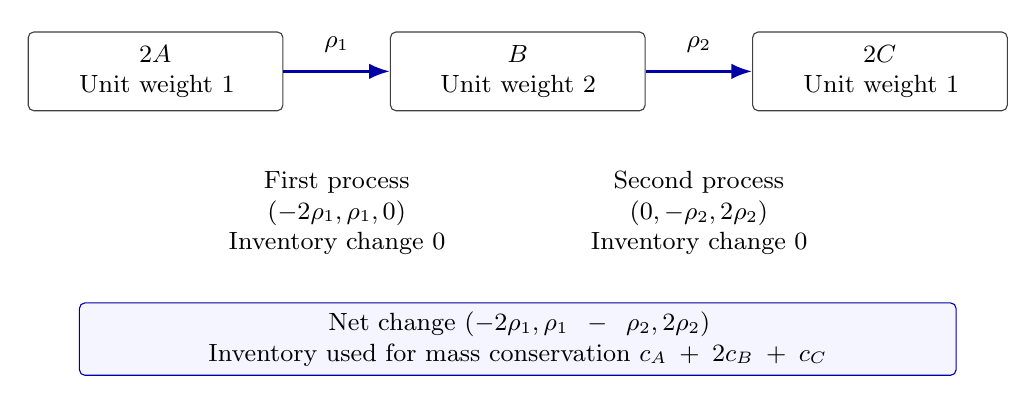
\begin{tikzpicture}[
    >=Latex,
    pool/.style={draw=black!75,fill=white,rounded corners=2pt,
        text width=3.0cm,minimum height=1.0cm,align=center,font=\small},
    process/.style={draw=blue!65!black,line width=1pt,->},
    account/.style={font=\small,align=center,text width=4.3cm}]
\node[pool] (a) at (0,0) {$2A$\\Unit weight $1$};
\node[pool] (b) at (4.6,0) {$B$\\Unit weight $2$};
\node[pool] (c) at (9.2,0) {$2C$\\Unit weight $1$};
\draw[process] (a)--(b) node[midway,above=3pt,font=\small] {$\rho_1$};
\draw[process] (b)--(c) node[midway,above=3pt,font=\small] {$\rho_2$};
\node[account] at (2.3,-1.8) {First process\\$(-2\rho_1,\rho_1,0)$\\Inventory change $0$};
\node[account] at (6.9,-1.8) {Second process\\$(0,-\rho_2,2\rho_2)$\\Inventory change $0$};
\node[draw=blue!65!black,fill=blue!4,rounded corners=2pt,
    text width=10.9cm,align=center,font=\small] at (4.6,-3.4)
    {Net change $(-2\rho_1,\rho_1-\rho_2,2\rho_2)$\\
    Inventory used for mass conservation $c_A+2c_B+c_C$};
\end{tikzpicture}
\endgroup

\caption{Hypothetical reaction accounting for three pools with inventory weights 1, 2, and 1. Each process redistributes the tracked inventory without creating or removing it.}
\label{fig:reactor_reaction_accounting}
\end{figure}

Two units of $A$ contain the same tracked inventory as one unit of $B$, and one unit of $B$ contains the same inventory as two units of $C$. Pool $B$ therefore acts as an intermediate: the first process produces it and the second consumes it. Its net concentration change depends on the difference between the two process rates even though each process individually preserves the weighted inventory.

If the process rates are $\rho_1$ and $\rho_2$, the scalar reaction contributions are
\[
\begin{aligned}
\dot c_A\big|_{\rm reaction}&=-2\rho_1,\\
\dot c_B\big|_{\rm reaction}&=\rho_1-\rho_2,\\
\dot c_C\big|_{\rm reaction}&=2\rho_2.
\end{aligned}
\]
The dot denotes a time derivative. These expressions describe reaction contributions only; hydraulic transport is not yet included. The same equations can be collected into a process-by-component matrix and a rate column,
\[
\nu_{\rm toy}=\begin{bmatrix}-2&1&0\\0&-1&2\end{bmatrix},\qquad
\rho_{\rm toy}=\begin{bmatrix}\rho_1\\\rho_2\end{bmatrix}.
\]
Transposing the stoichiometric matrix places the coefficients for each component in one row. Multiplication then reconstructs all three scalar rates at once:
\[
\nu_{\rm toy}^\top\rho_{\rm toy}
=\begin{bmatrix}-2&0\\1&-1\\0&2\end{bmatrix}
\begin{bmatrix}\rho_1\\\rho_2\end{bmatrix}
=\begin{bmatrix}-2\rho_1\\\rho_1-\rho_2\\2\rho_2\end{bmatrix}.
\]
For hypothetical rates of 3 and 1 in compatible amount-per-time units, the resulting contributions are $-6$, 2, and 2. Pool $B$ increases because its production exceeds its consumption. The positive changes in $B$ and $C$ do not mean that material has been created; they are accompanied by a corresponding loss from $A$.

The full activated sludge model uses the same convention. Its matrix orientation is fixed as
\begin{equation}
\equationname{Dimensions and orientation of the stoichiometric matrix}
\nu\in\mathbb{R}^{P\times F},\qquad P=28,\qquad F=20.
\label{eq:petersen_orientation}
\end{equation}
Row $p$ represents process $p$, and column $j$ represents component $j$. A negative entry $\nu_{pj}$ denotes consumption, a positive entry denotes production, and a zero entry means that the process has no direct stoichiometric contribution to that component. The coefficients also include the yields and constituent conversions required by the native component units.

For component $j$, the individual process contributions are $\nu_{1j}\rho_1$, $\nu_{2j}\rho_2$, and so on through $\nu_{28j}\rho_{28}$. Their sum gives the net reaction rate of that component. Writing the rate vector as $\rho(c,u)$ emphasizes that these rates depend on the current component state and operating inputs. For $\rho(c,u)\in\mathbb{R}^{28}$,
\begin{equation}
\equationname{Vector and scalar reaction contributions to component rates}
r_{\mathrm{reaction}}(c,u)=\nu^\top\rho(c,u),\qquad
r_{\mathrm{reaction},j}(c,u)=\sum_{p=1}^{28}\nu_{pj}\rho_p(c,u).
\label{eq:reaction_contribution}
\end{equation}

This formulation separates two different roles. Stoichiometry specifies the proportions in which components are consumed and produced; kinetics specifies how quickly those transformations proceed at a particular state. Increasing a biomass concentration can therefore change a process rate without changing the corresponding stoichiometric row. Likewise, changing aeration can alter oxygen limitation and thus process kinetics without changing the material accounting of the reaction itself.

A simple saturation factor makes this distinction concrete. If a limiting dissolved substrate has concentration $S$ and saturation constant $K_S>0$, then
\begin{equation}
\equationname{Monod substrate saturation factor}
\frac{S}{K_S+S}
\label{eq:saturation_example}
\end{equation}
equals one half when $S=K_S$, approaches zero as $S$ approaches zero, and approaches one as $S$ becomes large. For illustration, if both $S$ and $K_S$ equal 4 g COD m$^{-3}$, the factor is $4/(4+4)=0.5$. The concentration unit cancels because the numerator and denominator use the same constituent basis.

A representative growth expression combines a maximum specific growth rate, biomass abundance, and multiple limitation factors:
\begin{equation}
\equationname{Representative growth rate with substrate and oxygen limitation}
\rho_{\mathrm{growth}}=
\mu X\frac{S}{K_S+S}\frac{S_O}{K_O+S_O}.
\label{eq:representative_growth}
\end{equation}
Here $\mu$ is a maximum specific growth rate, $X$ is the associated biomass coordinate, and $K_O$ is an oxygen saturation constant. With hypothetical values $\mu=2$ d$^{-1}$, $X=10$ g biomass COD m$^{-3}$, a substrate factor of 0.5, and an oxygen factor of 0.25, the growth contribution is $2(10)(0.5)(0.25)=2.5$ g biomass COD m$^{-3}$ d$^{-1}$. The dimensionless limitation factors reduce the unrestricted contribution $\mu X=20$ to 2.5.

Equation~\eqref{eq:representative_growth} is illustrative rather than a replacement for the complete 28-process formulation. The actual model contains process-specific yields, inhibition terms, and storage dependencies from \citet{Henze2006} and \citet{Guerrero2011}. Its purpose here is to show why nonlinear interactions arise naturally. A hypothetical substrate concentration of $K_S/9$ gives a substrate factor of 0.1, whereas $9K_S$ gives a factor of 0.9. The substrate concentration changes by a factor of 81, but the saturation factor changes only by a factor of nine. Several such limitation terms and competing populations can act simultaneously. For this reason, a linear relationship between influent loading and effluent state is generally insufficient, and a surrogate may need to represent interactions without treating them as new stoichiometric laws.

\section{The steady-state reactor boundary}

The stoichiometric and kinetic relations describe transformation within the reactor. A reactor model also requires a boundary that accounts for material entering, leaving, and crossing that boundary through external transfer. The standalone prediction problem considers a completely mixed reactor at steady state. Perfect mixing makes the reactor concentration equal to the effluent concentration. The boundary includes hydraulic inflow and outflow, the 28 modeled reaction processes, and dissolved-oxygen transfer. It excludes a clarifier, solids return, and other external additions. These exclusions define the specific balance enforced in the reactor study; they do not imply that such processes are absent from wastewater treatment plants.

Let $c_{in}$ and $c_{out}$ denote the influent and effluent component vectors, and let $D>0$ denote the hydraulic dilution rate. For component $j$, hydraulic inflow contributes $Dc_{in,j}$ and hydraulic outflow contributes $-Dc_{out,j}$. Reaction contributes the sum of the 28 stoichiometric-rate products. Oxygen transfer contributes only to the dissolved-oxygen coordinate. The scalar steady-state balance is therefore
\[
0=Dc_{in,j}-Dc_{out,j}
+\sum_{p=1}^{28}\nu_{pj}\rho_p+\omega(e_{S_O})_j.
\]

Because $S_O$ is the first component in Equation~\eqref{eq:component_order}, the selector $e_{S_O}$ has a first coordinate equal to one and nineteen remaining coordinates equal to zero. The oxygen balance consequently contains the direct transfer term $+\omega$, while, for example, the ammonium balance does not. Written separately, the dissolved-oxygen equation is
\[
0=D(S_{O,in}-S_{O,out})+\sum_{p=1}^{28}\nu_{p,S_O}\rho_p+\omega.
\]
Every term in this equation is expressed as a numerical rate on the oxygen basis. The native basis changes with the component row. Collecting all twenty scalar balances gives
\begin{equation}
\equationname{Steady-state reactor component equation}
0=D(c_{in}-c_{out})+\nu^\top\rho(c_{out},u)+\omega e_{S_O}.
\label{eq:reactor_steady_balance}
\end{equation}
Equivalently, moving the hydraulic difference to the opposite side gives
\begin{equation}
\equationname{Effluent change expressed through reaction and oxygen transfer}
D(c_{out}-c_{in})=\nu^\top\rho(c_{out},u)+\omega e_{S_O}.
\label{eq:reactor_steady_difference}
\end{equation}
For an individual component,
$D(c_{out,j}-c_{in,j})=\sum_p\nu_{pj}\rho_p+\omega(e_{S_O})_j$.
The hydraulic term therefore has the same native component-unit-per-day basis as the corresponding reaction and transfer terms. A consistent numerical unit convention is required when the complete balance is treated as a vector equation.

The two operating inputs are HRT and the dimensionless aeration coordinate $u_{\mathrm{air}}$. HRT specifies how long the influent flow would require to replace one reactor volume. A 12-hour HRT corresponds to two reactor-volume replacements per day because $24/12=2$, so the associated dilution rate has units of inverse time. Oxygen transfer uses a different inverse-time coefficient, which becomes a concentration-per-time rate when multiplied by the oxygen concentration deficit. The adopted parameterization is
\begin{align}
\equationname{Hydraulic dilution rate from retention time}
D&=\frac{24\ \mathrm{h\,d}^{-1}}{\mathrm{HRT}},\label{eq:reactor_dilution}\\
\equationname{Oxygen-transfer coefficient from the aeration setting}
k_{La}&=(2+18u_{\mathrm{air}})\ \mathrm{d}^{-1},\label{eq:reactor_transfer_coefficient}\\
\equationname{Net oxygen-transfer rate and saturation concentration}
\omega&=k_{La}(S_{O,\mathrm{sat}}-S_{O,out}),\qquad
S_{O,\mathrm{sat}}=8.5\ \mathrm{g\ O_2\,m}^{-3}.
\label{eq:reactor_oxygen_transfer}
\end{align}
The dilution rate places hydraulic replacement on the same time basis as the biological process rates. The oxygen-transfer term depends on both the selected aeration setting and the difference between saturation and the actual reactor oxygen concentration.

For a hypothetical HRT of 12 h, Equation~\eqref{eq:reactor_dilution} gives $D=2$ d$^{-1}$. A component difference of 5 g m$^{-3}$ then corresponds to a net transformation or transfer of 10 g m$^{-3}$ d$^{-1}$ in that coordinate. For a hypothetical aeration setting of 1, the transfer coefficient is 20 d$^{-1}$. If dissolved oxygen is 2 g O$_2$ m$^{-3}$, the oxygen-transfer rate is 130 g O$_2$ m$^{-3}$ d$^{-1}$. These calculations illustrate the accounting implied by the equations; they are not simulated treatment outcomes.

Steady state means that the modeled inventories have zero time derivative under the stated equations and boundary. It does not establish that the steady state is unique, dynamically stable, or representative of a field-calibrated treatment plant. Sensitivity of operating choices to the process model therefore remains relevant even when the numerical balance closes \citep{Araujo2013}. A small residual can certify agreement with the specified equations at a returned state. It cannot certify that those equations completely describe a real wastewater system.

\section{From stoichiometry to mass conservation invariants}

The next step is to identify combinations of the component state that the modeled reactions cannot change. These combinations provide the mass conservation relations used later for physically constrained prediction. An invariant should not be interpreted as a concentration that remains unchanged throughout the plant. Ammonium, for example, can decrease while nitrate increases. What remains unchanged is an appropriate weighted combination of the included nitrogen pools, provided that the corresponding boundary flows and external sources are accounted for.

A stoichiometric invariant is therefore a linear combination of component concentrations whose reaction contribution is always zero. The hypothetical three-pool network provides the simplest example. Adding $A$, $B$, and $C$ without weights would incorrectly treat one unit of $B$ as if it contained the same inventory as one unit of $A$. The correct tracked inventory is
\[
I_{\rm toy}=c_A+2c_B+c_C.
\]
Substituting the scalar reaction rates gives
\[
\frac{d I_{\rm toy}}{dt}
=(-2\rho_1)+2(\rho_1-\rho_2)+(2\rho_2)=0.
\]
The $\rho_1$ and $\rho_2$ terms cancel independently. The equality therefore holds for every combination of process rates. For the hypothetical component change $(-6,2,2)^\top$, the weighted change is likewise $-6+2(2)+2=0$.

The invariant weights can also be derived rather than guessed. Let
$a=(a_A,a_B,a_C)^\top$ be an unknown coefficient column. Requiring each process to make zero weighted contribution gives
\[
\begin{aligned}
-2a_A+a_B&=0,\\
-a_B+2a_C&=0.
\end{aligned}
\]
The first equation gives $a_B=2a_A$, and the second gives $a_C=a_A$. Choosing $a_A=1$ yields $(1,2,1)^\top$. Choosing $a_A=3$ yields $(3,6,3)^\top$, which represents the same conservation law multiplied by three. These columns lie in the null space of $\nu_{\rm toy}$: they are component-space directions that the stoichiometric matrix sends to zero.

The full activated sludge model follows the same principle. If $a\in\mathbb{R}^{20}$ satisfies $\nu a=0$, then
\begin{equation}
\equationname{Zero reaction contribution to a stoichiometric invariant}
a^\top\nu^\top\rho=(\nu a)^\top\rho=0
\label{eq:individual_invariant}
\end{equation}
for every possible process-rate vector. Importantly, this identity does not depend on estimating the rates correctly or on choosing a particular operating condition. It follows from the stoichiometric accounting itself. Mass conservation-aware surrogate methods exploit this separation by preserving balances without reproducing all original kinetic calculations during prediction \citep{SturmWexler2020,SturmWexler2022,Hansen2024}.

The number of independent conservation relations depends on the number of independent reaction directions. In the toy system, neither stoichiometric row is a multiple of the other. If
$s(-2,1,0)+t(0,-1,2)=(0,0,0)$, the first coordinate requires $s=0$ and the third requires $t=0$. The two rows are therefore independent, so the matrix has rank two. With three component coordinates and two independent reaction directions, one independent invariant remains. This is the rank--nullity relation,
\[
\text{number of component coordinates}
=\text{rank}+\text{null-space dimension}.
\]
The free coefficient in the toy derivation is the arbitrary scale assigned to $a_A$. A basis is a set of independent vectors from which every vector in the space can be formed by weighted addition. Because the toy invariant space is one-dimensional, one basis column is sufficient.

For the full model, singular-value decomposition provides a numerically stable way to identify these directions. It factors a matrix into orthonormal directions and non-negative singular values. Orthonormal columns have unit Euclidean norm and zero scalar product with one another. A zero singular value marks a direction that the matrix sends to zero. For the toy matrix,
\[
\nu_{\rm toy}\nu_{\rm toy}^\top
=\begin{bmatrix}5&-1\\-1&5\end{bmatrix}.
\]
This square matrix has eigenvalues 4 and 6, giving two nonzero singular values, 2 and $\sqrt6$. The remaining component-space direction is the invariant direction. An eigenvalue describes the factor by which a square matrix stretches a corresponding direction, while singular values provide the analogous non-negative stretching magnitudes for matrices that may be rectangular.

For the full matrix, $U$ has dimension $28\times28$, $\Sigma$ has dimension $28\times20$, and $V$ has dimension $20\times20$. The rectangular matrix $\Sigma$ contains the singular values on its diagonal and zeros elsewhere. Their product reconstructs the original $28\times20$ stoichiometric matrix:
\begin{equation}
\equationname{Singular-value decomposition of the stoichiometric matrix}
\nu=U\Sigma V^\top.
\label{eq:stoichiometric_svd}
\end{equation}

Finite arithmetic requires a numerical definition of rank. A mathematically zero singular value may appear as a very small nonzero number after floating-point calculations. Rank is therefore determined using
\begin{equation}
\equationname{Numerical threshold for stoichiometric rank}
\tau_{\mathrm{rank}}=\max(P,F)\epsilon_{\mathrm{mach}}\|\nu\|_2.
\label{eq:stoichiometric_rank_threshold}
\end{equation}
Here $\epsilon_{\mathrm{mach}}$ is machine precision and $\|\nu\|_2$ is the largest singular value. The largest singular value establishes the scale of the matrix, while the dimension factor accounts for the size of the calculation. Under this criterion, the adopted stoichiometric model has rank 15. With 20 component coordinates, rank--nullity therefore gives five independent invariants.

The toy invariant $(1,2,1)^\top$ illustrates how the basis is normalized. Its Euclidean length is $\sqrt{1^2+2^2+1^2}=\sqrt6$, so its unit-length form is
\[
V_{0,\rm toy}=\frac1{\sqrt6}\begin{bmatrix}1\\2\\1\end{bmatrix}.
\]
Its scalar product with each stoichiometric row is zero:
$(-2+2+0)/\sqrt6=0$ and $(0-2+2)/\sqrt6=0$.
For the full model, five orthonormal right singular vectors perform the same role. Let $V_0\in\mathbb{R}^{20\times5}$ contain the right singular vectors spanning $\operatorname{null}(\nu)$, and define
\begin{equation}
\equationname{Orthonormal mass conservation operator from the null space}
A=V_0^\top\in\mathbb{R}^{5\times20}.
\label{eq:invariant_basis_definition}
\end{equation}
The operator then satisfies
\begin{equation}
\equationname{Null-space and orthonormality identities of the invariant operator}
A\nu^\top=0,\qquad AA^\top=I_5.
\label{eq:invariant_basis_properties}
\end{equation}
The first identity states that every invariant row has zero contribution from every reaction direction. The second states that the invariant rows have unit length and are mutually orthogonal. These rows need not correspond one-to-one with named elemental inventories. Their purpose is to provide a fixed, numerically scaled basis for the same conservation space.

The matrix orientation is important. Because the processes are rows of $\nu$, the component combinations that define conservation lie in the right null space of $\nu$. By contrast, the right null space of $\nu^\top$ lies in process coordinates and describes dependencies among process contributions. These are different objects. Checking matrix dimensions prevents the two interpretations from being confused.

Reaction conservation alone, however, is not enough to establish conservation across an open reactor boundary. The inflow, outflow, and external transfer terms must also be considered. For invariant row $h$, multiply the component balance by $A_{hj}$ and sum over the twenty components:
\[
\begin{aligned}
D\sum_{j=1}^{20}A_{hj}(c_{out,j}-c_{in,j})
&=\sum_{p=1}^{28}\rho_p\sum_{j=1}^{20}A_{hj}\nu_{pj}
+\omega\sum_{j=1}^{20}A_{hj}(e_{S_O})_j\\
&=0+\omega A_{h1}.
\end{aligned}
\]
The reaction contribution vanishes because of the invariant construction. The oxygen-transfer selector leaves only the oxygen-column coefficient. Premultiplying Equation~\eqref{eq:reactor_steady_difference} by $A$ gives the same result in vector form:
\begin{equation}
\equationname{Reactor invariant equation including oxygen transfer}
D A(c_{out}-c_{in})=\omega A e_{S_O}.
\label{eq:invariant_boundary_balance}
\end{equation}
Reaction cancellation and external-forcing compatibility are therefore separate requirements.

The distinction can again be seen in the toy system. Adding one unit directly to pool $A$ corresponds to a forcing column $(1,0,0)^\top$. Its invariant product is $1/\sqrt6$, so the forcing changes the tracked inventory. A forcing column $(-2,1,0)^\top$, in contrast, has invariant product $(-2+2)/\sqrt6=0$ and lies within the reaction-change space. This abstract example illustrates why an external forcing must be checked against the conservation space rather than assumed to preserve it.

The range of a matrix is the set of vectors that it can produce by multiplication with all possible coordinate columns. Any forcing in $\operatorname{range}(\nu^\top)$ can be written as a combination of reaction-change directions and is therefore annihilated by every invariant row. For the adopted stoichiometric matrix, the dissolved-oxygen selector satisfies this condition. There exists a process-coordinate vector $\lambda_O\in\mathbb{R}^{28}$ such that
\begin{equation}
\equationname{Compatibility of oxygen forcing with mass conservation}
e_{S_O}=\nu^\top\lambda_O,\qquad
Ae_{S_O}=A\nu^\top\lambda_O=0.
\label{eq:oxygen_forcing_compatibility}
\end{equation}
The coordinates in $\lambda_O$ establish a subspace relation only. They do not mean that aeration is itself a biological process or that the entries of $\lambda_O$ are non-negative process rates.

Because $Ae_{S_O}=0$, Equation~\eqref{eq:invariant_boundary_balance} reduces to
$D A(c_{out}-c_{in})=0$. Since $D>0$,
\begin{equation}
\equationname{Equality of influent and effluent invariant inventories}
Ac_{out}=Ac_{in}.
\label{eq:reactor_invariant_equality}
\end{equation}
This equality follows jointly from the stoichiometric model, the direction of the oxygen forcing, and the stated reactor boundary. It should not be transferred unchanged to a system with an unaccounted phosphorus dose, sludge withdrawal, or another external source that changes the conserved inventories.

More generally, let $g$ denote an additional component source expressed on a concentration-per-time basis. Its contribution to invariant row $h$ is $\sum_jA_{hj}g_j$. Dividing by the positive dilution rate converts that contribution to a concentration-equivalent invariant change. When aeration remains compatible,
\begin{equation}
\equationname{Invariant inventory change with an external source}
A(c_{out}-c_{in})=D^{-1}Ag.
\label{eq:general_invariant_source}
\end{equation}
A phosphate addition with a nonzero phosphorus-inventory contribution would therefore change the right-hand side. Imposing the original influent equality in such a system would incorrectly remove a real external contribution. This example illustrates a general principle used throughout the dissertation: a physical constraint must be derived from the actual model boundary, not selected merely because it produces a convenient statistical result.

All numerical calculations use the full-precision operator. Its construction is checked through $A\nu^\top$, $AA^\top-I_5$, and $Ae_{S_O}$. Rounded coefficients displayed for interpretation cannot replace the original operator in computation. Any nonsingular row transformation $T$ produces $A'=TA$ and defines the same equality set, but an arbitrary transformation changes the numerical scale of residuals. The orthonormal construction therefore fixes both the invariant space and the scaling used for mass conservation diagnostics.

\section{Reaction progress and the feasible state geometry}

The invariant relation describes what cannot change. A complementary view describes the directions along which the component state can change while preserving those invariants. This reaction-progress view is useful because it connects the mechanistic stoichiometric model to the geometry of the feasible states later used for projection.

Consider again the hypothetical three-pool system. Suppose the first process advances by one unit and the second by one half-unit on a compatible concentration-equivalent basis. The accumulated component changes are
\[
\begin{aligned}
\Delta c_A&=-2(1)+0(0.5)=-2,\\
\Delta c_B&=1(1)-1(0.5)=0.5,\\
\Delta c_C&=0(1)+2(0.5)=1.
\end{aligned}
\]
Their weighted sum is $-2+2(0.5)+1=0$. Starting from the hypothetical state $(8,1,1)^\top$ gives $(6,1.5,2)^\top$, and both states have weighted inventory 11. The accumulated progress is conceptually different from an instantaneous process rate: multiplying a rate by an appropriate time scale produces a concentration-equivalent state change.

For the steady reactor, that natural time scale is $D^{-1}$. Using
$\omega e_{S_O}=\nu^\top(\omega\lambda_O)$ allows reaction and compatible oxygen transfer to be represented in the same component-change space. Rearranging the steady-state balance gives
\begin{equation}
\equationname{Reaction-progress coordinates for the effluent change}
c_{out}-c_{in}=\nu^\top r,\qquad
r=D^{-1}(\rho+\omega\lambda_O).
\label{eq:reaction_progress_coordinates}
\end{equation}
The vector $r$ provides one set of process-space coordinates for the total component change. It should not be interpreted as a unique reconstruction of the biological reaction rates. The matrix $\nu^\top$ has rank 15 but 28 columns, so multiple process-coordinate vectors can produce the same component change. Moreover, $r$ contains the algebraic representation of oxygen transfer. Its entries are therefore not independently measured reaction extents or microbial activities.

A mass-conserving component change also need not be represented using the original process coordinates. In the toy system, every admissible change $v$ satisfies
$v_A+2v_B+v_C=0$. Two independent unit-length directions satisfying this condition are
\[
z_1=\frac1{\sqrt5}\begin{bmatrix}-2\\1\\0\end{bmatrix},\qquad
z_2=\frac1{\sqrt{30}}\begin{bmatrix}1\\2\\-5\end{bmatrix}.
\]
Their invariant products are zero, their mutual scalar product is zero, and both have unit length. Thus
$Z_{\rm toy}=[z_1\ z_2]$ is an orthonormal basis of the two-dimensional change space. Any toy-state change that preserves the weighted inventory can be written as
$v=z_1q_1+z_2q_2$.

The change basis and the invariant basis answer complementary questions. The invariant rows identify combinations that cannot change. The columns of $Z$ identify directions along which the state can move without changing those combinations. In the full model, five independent invariant rows leave fifteen independent change directions. Let
$Z\in\mathbb{R}^{20\times15}$ contain orthonormal columns spanning $\operatorname{null}(A)$. The corresponding subspace relation is
\begin{equation}
\equationname{Equivalent reaction and invariant-null spaces}
\operatorname{range}(\nu^\top)=\operatorname{null}(A),\qquad
AZ=0,\qquad Z^\top Z=I_{15}.
\label{eq:reaction_invariant_subspaces}
\end{equation}
Every component change satisfying the conservation equalities can therefore be written uniquely as $Zq$ for some $q\in\mathbb{R}^{15}$ in the selected orthonormal basis. These coordinates describe admissible material redistribution. They do not identify a unique sequence of the 28 kinetic processes responsible for that redistribution.

The same relation defines the feasible component states used in prediction. For sample $i$, the invariant target is
$b_i=Ac_{in,i}$. A physically admissible effluent must satisfy the five invariant equalities and the twenty non-negativity bounds:
\begin{equation}
\equationname{Component-state set satisfying mass conservation and non-negativity}
\mathcal{F}_i=\{c\in\mathbb{R}^{20}\mid Ac=b_i,\ c\geq0\}.
\label{eq:reactor_feasible_set}
\end{equation}
The equality $Ac=b_i$ defines a 15-dimensional affine space before the concentration bounds are applied. An affine space is a linear change space translated by a fixed reference state; the influent provides one such reference here. Intersecting that affine space with the non-negative orthant retains only states whose component concentrations are all non-negative.

The resulting set has several useful properties. It is closed because the equalities and inequalities include their boundary points. It is convex because any weighted average of two feasible states, using weights between zero and one, preserves both the invariant target and component non-negativity. It is also nonempty whenever the influent is non-negative, because the influent itself satisfies $Ac_{in,i}=b_i$ and provides a feasible anchor.

The toy example makes this geometry visible. For the hypothetical influent $(8,1,1)^\top$, the conservation condition is
$c_A+2c_B+c_C=11$, together with
$c_A,c_B,c_C\geq0$. If only one pool is nonzero, the three boundary states are
$(11,0,0)^\top$, $(0,5.5,0)^\top$, and $(0,0,11)^\top$. The feasible region is the triangle connecting these states within the inventory plane. The state $(6,1.5,2)^\top$ lies inside this triangle. The state $(12,-0.5,0)^\top$ lies in the same inventory plane because $12-1=11$, but it is not physically admissible because one coordinate is negative. Mass conservation selects the plane; non-negativity selects the admissible portion of that plane.

Figure~\ref{fig:reactor_feasible_triangle} shows the same region using $c_A$ and $c_B$ as plotting axes. The conservation equation supplies the third coordinate through
$c_C=11-c_A-2c_B$, so every plotted point still represents a complete three-component state.

\begin{figure}[htbp]
\centering
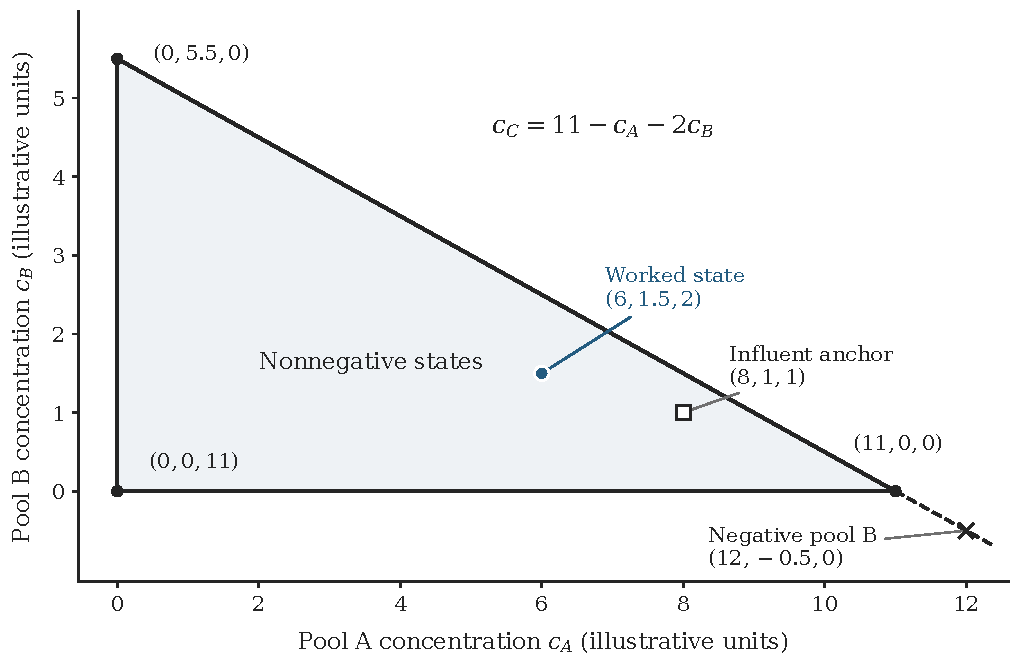
\includegraphics[width=0.93\textwidth]{ch3_concept_feasible_triangle.pdf}
\caption{Hypothetical non-negative states for the weighted inventory $c_A+2c_B+c_C=11$. The shaded triangle includes its boundary. Full state labels retain the third component even though only two coordinates are plotted.}
\label{fig:reactor_feasible_triangle}
\end{figure}

The sloping edge corresponds to $c_C=0$, while the two coordinate edges correspond to $c_A=0$ or $c_B=0$. All three components are positive in the interior, allowing the same conserved inventory to be distributed among them in many different proportions. The cross-marked point preserves the weighted inventory but has a negative $B$ concentration. The figure therefore shows that conservation and concentration bounds define different requirements.

A two-component example makes the same point even more directly. Suppose conservation fixes
$c_1+c_2=10$. The equality alone permits states such as $(-1,11)$, $(4,6)$, and $(12,-2)$. Non-negativity reduces this infinite line to the segment between $(0,10)$ and $(10,0)$. Simply clipping $(-1,11)$ to $(0,11)$ removes the negative concentration but changes the conserved sum from 10 to 11. Enforcing the equality and enforcing non-negativity are therefore not interchangeable operations; simultaneous enforcement requires their intersection.

The geometry also clarifies the limitation of a physically admissible prediction. Many non-negative component states can share the same five invariant values. A state with an incorrect distribution between ammonium and nitrate may still satisfy all conservation equalities. The same can occur for an implausible biomass concentration. The feasible set therefore establishes the declared material accounting and sign restrictions, but it does not establish that the complete 28-process kinetics balance hydraulics and aeration at that state. This distinction is central to the constraint methods of \citet{KircherVotsmeier2025} and to the broader physical-consistency perspective of \citet{Valente2025}.

\section{Reported water quality quantities and hidden component errors}

Engineering decisions are often communicated through aggregate quantities such as COD, TN, TP, and TSS rather than through the complete 20-component state. These quantities are important summaries, but they are calculated from the component state after prediction. The distinction matters because aggregation can hide component-level errors and because a reporting total is not necessarily a conserved inventory.

Using the coefficients in Table~\ref{tab:component_basis_composites}, the four reported quantities are
\[
\begin{aligned}
\mathrm{COD}={}&S_F+S_A+S_I+X_I+X_S+X_H+X_{PAO}\\
&+X_{PHA}+X_{AOB}+X_{NOB},\\[2pt]
\mathrm{TN}={}&S_{NH4}+S_{NO2}+S_{NO3}+0.01S_I+0.02X_I\\
&+0.07(X_H+X_{PAO}+X_{AOB}+X_{NOB}),\\[2pt]
\mathrm{TP}={}&S_{PO4}+0.01X_I+0.02(X_H+X_{PAO}+X_{AOB}+X_{NOB})\\
&+X_{PP}+X_{MeP}/4.87,\\[2pt]
\mathrm{TSS}={}&0.75(X_I+X_S)+0.90(X_H+X_{PAO}+X_{AOB}+X_{NOB})\\
&+3.23X_{PP}+0.60X_{PHA}+X_{MeP}+X_{MeOH}.
\end{aligned}
\]
Each coefficient converts a component from its native basis to the output basis of the corresponding reported quantity. For example, the factor 0.07 has units of g nitrogen per g biomass COD. Multiplying it by $X_H$ therefore gives a nitrogen concentration. Likewise, the factor 3.23 converts stored phosphorus to its suspended-solids contribution. Every term within one reported quantity is consequently expressed on a common basis before being summed.

A sparse hypothetical state containing only
$X_H=100$ g COD m$^{-3}$ and
$X_{PP}=2$ g P m$^{-3}$ gives
\[
\begin{aligned}
\mathrm{COD}&=100, &\mathrm{TN}&=0.07(100)=7,\\
\mathrm{TP}&=0.02(100)+2=4,
&\mathrm{TSS}&=0.90(100)+3.23(2)=96.46.
\end{aligned}
\]
Each result has its own constituent unit. The example illustrates how reporting coefficients combine different state components; it is not intended to represent a reactor steady state.

The same four sums can be written compactly using a fixed reporting matrix:
\begin{equation}
\equationname{Component-to-water-quality reporting map}
y=I_{comp}c,\qquad
y=(\mathrm{COD},\mathrm{TN},\mathrm{TP},\mathrm{TSS})^\top,\qquad
I_{comp}\in\mathbb{R}^{4\times20}.
\label{eq:component_composite_map}
\end{equation}
The first row contains the COD coefficients, the second the TN coefficients, and so forth. The rows convert the component state to g COD m$^{-3}$, g N m$^{-3}$, g P m$^{-3}$, and g TSS m$^{-3}$. Because all reporting coefficients are non-negative, a non-negative component state necessarily gives non-negative reported quantities.

A reported total should not, however, be confused with a conserved inventory. Dissolved dinitrogen has zero weight in the adopted TN reporting map. A hypothetical transfer of 3 g N m$^{-3}$ from nitrate to dissolved dinitrogen therefore reduces reported TN by 3 g N m$^{-3}$ even though the complete modeled nitrogen inventory can remain unchanged. A phosphorus reporting row may coincide more closely with a modeled phosphorus inventory, but that relationship must still be checked from the coefficients. The word ``total'' alone does not establish conservation.

The reporting coefficients also make the constituent conversions transparent. Under the adopted map, a hypothetical
$X_H=100$ g COD m$^{-3}$ contributes
100 g COD m$^{-3}$ to COD,
7 g N m$^{-3}$ to TN,
2 g P m$^{-3}$ to TP, and
90 g TSS m$^{-3}$ to TSS.
A hypothetical
$X_{PP}=2$ g P m$^{-3}$ contributes
2 g P m$^{-3}$ to TP and
6.46 g TSS m$^{-3}$ to TSS.
These values arise from fixed reporting assumptions rather than from the surrogate model or from an observed treatment outcome.

The main consequence of aggregation is that different component errors can cancel. Equal and opposite errors in ammonium and nitrate disappear in reported TN because both have unit nitrogen weights. A negative ammonium prediction can even be obscured by a sufficiently large nitrate prediction. Likewise, biomass and substrate errors can compensate in COD while remaining visible in TSS because their solids conversion factors differ. Accurate COD, TN, TP, and TSS values therefore do not establish either an accurate or a physically admissible 20-component state.

The reporting map and the invariant operator consequently answer different questions. The reporting map summarizes treatment performance in familiar engineering quantities. The invariant operator tests whether the component state satisfies the declared material accounting. Neither one reconstructs the detailed component distribution lost through aggregation. Component prediction, composite reporting, mass conservation, and non-negativity must therefore remain separate objects of assessment.

\section{Mixing and spatial transport as model boundaries}

The standalone reactor model assumes one completely mixed concentration for each component. This removes spatial coordinates from the reactor state and allows the treatment response to be represented by one component vector. The assumption is a modeling boundary rather than a statement that every biological treatment unit is spatially uniform. Biofilms, trickling filters, and incompletely mixed aerated vessels can exhibit concentration gradients and transport limitations \citep{Wik2003,Zhang1994,SadinoRiquelme2023}. Recognizing these effects helps define what the mixed-reactor surrogate does and does not represent.

A small spatial control volume illustrates the additional accounting required when concentrations vary in space. For one component, let $V$ denote the fixed control-volume size and $\bar c$ its average concentration. Let
$F_{\rm adv,in}$ and $F_{\rm adv,out}$ denote advective mass flow rates, and let
$F_{\rm diff,in}$ and $F_{\rm diff,out}$ denote diffusive mass flow rates. The finite-volume balance is
\begin{equation}
\equationname{Control-volume component equation with transport and reaction}
V\frac{\mathrm d\bar c}{\mathrm dt}
=F_{\rm adv,in}-F_{\rm adv,out}
+F_{\rm diff,in}-F_{\rm diff,out}+Vr.
\label{eq:teaching_spatial_control_volume}
\end{equation}
The quantity $r$ is the net reaction production rate per unit volume and becomes negative when the component is consumed. Every term on the right-hand side has units of component mass per time.

For a hypothetical volume of 2 m$^3$, advective inflow and outflow of 5 and 3 g d$^{-1}$, diffusive inflow and outflow of 2 and 0 g d$^{-1}$, and total reaction consumption of 3 g d$^{-1}$, the net accumulation is
$5-3+2-0-3=1$ g d$^{-1}$. Dividing by the control-volume size gives
$\mathrm d\bar c/\mathrm dt=0.5$ g m$^{-3}$ d$^{-1}$. The example shows why a local concentration change cannot be inferred from the reaction term alone: transport can be equally important.

In a one-dimensional domain with coordinate $z$, the advective flux is $vc$ and the diffusive flux is
$-D_z\partial c/\partial z$, where $v$ is velocity and $D_z$ is a dispersion or diffusion coefficient. Dividing the balance of a thin slice by its volume and taking the limit as its thickness approaches zero gives
\begin{equation}
\equationname{One-dimensional advection-diffusion-reaction component equation}
\frac{\partial c_j}{\partial t}
=-\frac{\partial(v c_j)}{\partial z}
+\frac{\partial}{\partial z}
\left(D_z\frac{\partial c_j}{\partial z}\right)
+\sum_{p=1}^{n_p}\nu_{pj}\rho_p+s_j.
\label{eq:teaching_spatial_balance}
\end{equation}
The first two terms describe spatial transport, the summation retains the same component-wise reaction accounting used in the mixed reactor, and $s_j$ represents a specified external source per unit volume. Boundary conditions then determine how material enters and leaves the spatial domain. Applying an invariant weighted sum can cancel compatible reaction terms, but transport and external-source contributions remain in the overall balance.

This formulation shows how the same theoretical ideas can extend beyond a completely mixed reactor without implying that a spatial reactor is added to the present study. Chapter~\ref{ch:plant} instead uses a sequence of mixed biological reactors and a layered clarifier. The reactor stages represent distinct treatment conditions, while the clarifier layers represent solids transport and storage. Their boundaries are different, and those differences must be respected when the connected plant constraints are derived.

\section{A common basis for assessing surrogate responses}

The preceding sections establish a common component representation for the rest of the dissertation. The mechanistic model supplies the reference treatment state. A statistical surrogate approximates that state from the influent and operating controls. Projection adjusts the prediction so that it lies within the specified physical set. Interpretation examines how the prediction is produced, and optimization uses the returned response to select operating conditions. The same component state therefore connects prediction, physical enforcement, interpretation, and decision assessment.

This connection is useful because these questions require different evidence. Prediction error measures agreement with the mechanistic reference. Physical admissibility concerns the imposed equalities, bounds, and inventories. Interpretability concerns the structure of the fitted response and how that structure changes through subsequent transformations. Operating quality concerns the treatment outcome obtained at the selected controls. One type of evidence cannot substitute for another.

The same distinction applies when raw and projected states are compared. A paired raw--projected assessment keeps the fitted learner fixed and isolates the effect of physical enforcement. Comparing separately trained predictors also includes differences in model structure, hyperparameter selection, and fitting. The structured regression developed later introduces additional intermediate states, including coupled and affine predictions, so that the origin of a change can be traced through the complete prediction procedure.

At plant scale, the accounting extends across locations. The mixer, reactor stages, clarifier outlets, and stored solids each contribute part of the connected response. Location-specific errors show where joint projection changes the predicted state, while plant-level summaries describe the overall approximation. The quantities used in the intended operating decision then determine which parts of that response require the closest scrutiny \citep{BhosekarIerapetritou2018,McBride2019}.

Table~\ref{tab:claim_evidence} summarizes this assessment logic. Input transformations, learned scales, regularization, and hyperparameter selection use development information. Reserved responses supply the final prediction assessment. This separation applies to the complete procedure, including both the fitted statistical model and the constrained calculation that follows it \citep{Kaufman2012}.

\begin{table}[htbp]
\centering\small
\caption{Assessment questions and the evidence used to connect surrogate responses to engineering decisions.}
\label{tab:claim_evidence}
\begin{tabular}{>{\raggedright\arraybackslash}p{0.24\textwidth}>{\raggedright\arraybackslash}p{0.39\textwidth}>{\raggedright\arraybackslash}p{0.27\textwidth}}
\toprule
Assessment question & Evidence & Engineering quantity\\
\midrule
Predictive agreement & Held-out component and composite errors with defined scales & Substrate, nutrients, biomass, and solids concentrations\\
Physical admissibility & Equality residuals, non-negativity checks, and inventory bounds & Conserved inventories and feasible component states\\
Sample efficiency & Common learning curves and variation across partitions & Error at the available simulation budget\\
Inspectable structure & Named coefficient blocks, physical units, and complete-response sensitivities & Dependence on influent and operating inputs\\
Operating quality & Independent mechanistic evaluation at selected controls & Treatment outcomes, engineering requirements, and objective values\\
Computational effort & Development, search, prediction, projection, and verification times & Time required to deliver an evaluated decision\\
\bottomrule
\end{tabular}
\end{table}

The numerical checks are reported using explicit tolerances and residual definitions. The equalities define the mathematical constraints; the residuals quantify how closely the returned numerical state satisfies them. Reporting these quantities in their original units or under a clearly defined scaling makes the physical calculation open to inspection \citep{Boyd2004,BuzziFerraris2013}. Chapters~\ref{ch:projection}--\ref{ch:plant} apply this common basis to the standalone reactor benchmark, the structured regression, and the connected-plant optimization study.
\chapter{Learning the Reactor Response and Enforcing Physical Admissibility}
\label{ch:projection}

\section{Rationale}

Repeated activated sludge calculations are needed when influent conditions or operating settings must be compared. A statistical surrogate can reduce the cost of these calculations by learning the reactor response from simulated cases and then approximating that response at new inputs. Its engineering usefulness, however, depends on more than prediction speed. It also depends on what the surrogate predicts, how closely those predictions reproduce the complete treatment state, and whether the returned state satisfies the physical requirements imposed by the reactor model.

The activated sludge response considered here is inherently multicomponent. Organic substrate, nitrogen species, phosphorus, biomass, and solids all contribute to treatment performance and to the material accounting of the reactor \citep{Henze2006}. Reported quantities such as COD, TN, TP, and TSS summarize parts of this response, but they do not uniquely determine the underlying component state. Two effluents can, for example, have the same TN while containing different proportions of ammonium, nitrite, nitrate, and biomass-bound nitrogen. A model can therefore predict a reported total accurately while misrepresenting the component distribution that produced it. For this reason, the complete component state is retained as the primary prediction target throughout this chapter.

The first research gap concerns comparative evidence for this complete activated sludge response. Existing studies support useful but different prediction tasks. The soft sensor of \citet{Ching2022} estimates oxygen demand from available measurements, while \citet{Wang2025} compare methods for effluent TN prediction. The structured reactor study of \citet{Selerio2026} instead retains the complete effluent component state. These contributions establish the value of data-driven activated sludge prediction, but their results cannot by themselves determine which learning method best approximates the same full reactor response. Such a comparison requires a common prediction target, identical influent and operating inputs, the same assessment cases, and the same error scales. Without this common basis, differences in the task can be mistaken for differences in learner performance.

The amount of available training data is part of the same problem. Mechanistic simulation is required to generate the learning cases, and this simulation budget may itself be limited. A flexible learner can become highly accurate when many cases are available without necessarily being the best choice at a smaller design size. The learning-curve review of \citet{VieringLoog2023} shows why performance should be examined across data budgets rather than at only one training size. The broader tabular comparisons of \citet{Borisov2024} and \citet{ShwartzZiv2022} likewise support evaluating several learning families rather than assuming that one class is consistently preferable. In the present setting, this comparison must preserve the substrate, nutrient, biomass, and solids coordinates that matter to subsequent reactor analysis.

Prediction outside the sampled influent and operating ranges introduces a further distinction. A held-out case drawn from the same input ranges tests interpolation within the declared learning domain. An unfamiliar loading or operating condition tests a different use of the surrogate. This distinction becomes important when a fitted model is used to explore alternatives rather than only reproduce familiar conditions. The present study therefore evaluates learning-domain and exterior inputs separately. A low held-out error within the sampled range does not establish accurate extrapolation, and a physically admissible prediction outside that range does not establish that its component distribution is correct \citep{KircherVotsmeier2025,Selerio2026}.

The second research gap concerns physical enforcement on these same reactor predictions. Ordinary regression is designed to approximate the statistical response. It does not necessarily preserve the sample-specific material inventories or prevent negative concentrations at a new input. Physical guidance during fitting and explicit constraints on the final returned state address different parts of this problem \citep{Kashinath2021,Hansen2024}. A prediction can satisfy the adopted balance equations while containing a negative component. Conversely, replacing a negative value by zero can destroy a balance that the original prediction happened to satisfy. Mass conservation and non-negativity must therefore be checked together on the same returned component state.

The projection developed by \citet{KircherVotsmeier2025} provides a way to enforce these two requirements simultaneously. The remaining question for the present study is not whether such a projection can be written, but how a common projection behaves when applied to a broad set of activated sludge learners. Different predictors may produce different raw error structures, different negative-component patterns, and different departures from the invariant balances. Applying one projection across them therefore makes it possible to separate the behavior of the statistical learner from the behavior of the enforcement procedure.

Physical compliance is only one part of this assessment. Projection changes the predicted component vector, and that adjustment can redistribute error among its entries. The same redistribution also changes COD, TN, TP, and TSS, because those reported quantities are calculated from the projected components rather than from an independent prediction. The species-weighted correction of \citet{SturmSilva2024} illustrates why the metric used to define an adjustment matters. A correction that improves one nutrient quantity can worsen another constituent or solids measure. A feasible-state count alone therefore cannot establish whether the adjustment improves treatment prediction. Component errors, composite treatment errors, and physical diagnostics must be examined together.

The complete prediction procedure also has a computational cost. A surrogate intended for repeated operating calculations should be timed not only at the raw statistical inference stage, but also after the physical enforcement needed to produce its final returned state. Large adjustments can indicate substantial disagreement between the raw prediction and the imposed physical relations, whereas small adjustments indicate only proximity to those relations and do not establish accurate reaction behavior. By pairing each raw prediction with its projected counterpart, the study can examine statistical error, physical compliance, displacement, and prediction cost without changing the fitted learner. This distinction follows the broader need to evaluate approximation quality and computational usefulness together in surrogate modeling \citep{BhosekarIerapetritou2018}.

Accordingly, this chapter addresses the first and second research questions in Section~\ref{sec:research_questions}. It first compares complete reactor predictions across learning methods, simulation budgets, and input-domain conditions. It then applies a common projection to those same predictions and measures what the enforcement changes. The contribution is an activated sludge benchmark that separates learner performance from physical enforcement while showing how the two interact in practice. The study does not introduce a new projection principle, and it does not assume that physical enforcement improves every error measure. Its purpose is to provide a defensible basis for selecting a learner and a projection procedure under specified data availability, treatment priorities, and operating ranges.

\section{Theory}

\subsection{Reactor inputs and raw predictions}

Each surrogate receives the operating conditions and influent component concentrations that define one reactor case. For sample $i$, the two operating values are listed first, followed by the twenty influent concentrations in the component order established in Chapter~\ref{ch:foundations}. The input therefore begins with $(\mathrm{HRT}_i,u_{\mathrm{air},i},S_{O,in,i},S_{F,in,i})$ and continues through the remaining influent coordinates to $X_{MeOH,in,i}$. The component definitions and units are fixed before any statistical learner is fitted.

Writing the operating vector and influent vector as columns gives the complete surrogate input
\begin{equation}
\equationname{Reactor surrogate inputs from operation and influent concentrations}
x_i=(u_i^\top,c_{in,i}^\top)^\top\in\mathbb{R}^{22},\qquad
u_i=(\mathrm{HRT}_i,u_{\mathrm{air},i})^\top.
\label{eq:surrogate_input_vector}
\end{equation}
Thus, every fitted learner receives the same twenty-two quantities for each case.

A fitted surrogate is represented by $f_m$, where the subscript $m$ identifies the learning method. It maps the twenty-two inputs to the twenty effluent component concentrations. For component $j$, the scalar prediction can be written as
$c_{raw,ij}^{(m)}=f_{m,j}(x_{i1},\ldots,x_{i22})$.
The superscript $(m)$ identifies the model and is not an exponent. Collecting the twenty scalar outputs gives the raw component prediction
\begin{equation}
\equationname{Raw component-state prediction from a fitted surrogate}
c_{raw,i}^{(m)}=f_m(x_i)\in\mathbb{R}^{20}.
\label{eq:surrogate_raw_state}
\end{equation}

This raw state is assessed in the physical units returned by the surrogate. A post-prediction projection then produces a second state for the same sample. The raw and projected predictions therefore correspond to the same fitted learner, the same input, the same preprocessing, and the same assessment case. Their paired comparison isolates the effect of physical enforcement from differences in model training or data partitioning \citep{SturmSilva2024,KircherVotsmeier2025}.

\subsection{Statistical response models}

\subsubsection{Boosting and randomized tree ensembles}

XGBoost represents a response as an additive sequence of regression trees. Each tree partitions the input space through a sequence of comparisons and assigns the value associated with the terminal region reached by the input. For one effluent component, an additive tree model can be written as
\[
f_j(x)=b_j+\beta_1h_{1j}(x)+\beta_2h_{2j}(x)+\cdots+\beta_Th_{Tj}(x),
\]
where $b_j$ is a baseline, $h_{tj}(x)$ is the response of tree $t$, and $\beta_t$ controls that tree's contribution. The equivalent summation form is
$b_j+\sum_{t=1}^T\beta_th_{tj}(x)$.
For example, a baseline of 10 with tree contributions of $-2$ and 1 gives a final prediction of 9.

Successive trees are fitted to reduce error remaining from the current ensemble, while regularization discourages unnecessarily complex fits. Because tree splits divide the input domain into regions, the resulting model can represent nonlinearities and interactions without requiring those relationships to be specified in advance. The regularized boosting framework of \citet{ChenGuestrin2016} motivates the inclusion of XGBoost as a flexible tabular comparator.

LightGBM is also a gradient-boosted tree method, but it grows trees through leaf-wise expansion. The algorithm preferentially expands a leaf when doing so produces a larger loss reduction, allowing additional model detail to concentrate in regions where the current fit remains poor. Its learning rate, leaf count, and minimum leaf support control how closely the ensemble follows the training response. The efficiency-oriented design of \citet{Ke2017} makes this method particularly relevant when model fitting must be repeated across several nested validation partitions.

CatBoost uses symmetric boosted trees together with a Bayesian bootstrap in the present regression setting. At each depth, the same splitting condition is applied across all nodes of a symmetric tree. This restriction gives CatBoost a different approximation structure from the leaf-wise trees of LightGBM. Although the work of \citet{Prokhorenkova2018} emphasizes categorical-feature handling and boosting bias, the present reactor benchmark evaluates the method using continuous inputs only.

Adaptive boosting regression combines shallow trees while placing greater emphasis on observations that remain difficult to predict. The base learners used here are depth-three trees. The number of estimators, learning rate, and loss function determine how strongly the ensemble responds to poorly fitted cases. The regression extension developed by \citet{Drucker1997} provides the basis for this comparator.

These four boosting methods are fitted separately for each effluent component. Within a given method, all twenty component regressors use one shared selected hyperparameter vector. This preserves a common model setting across the complete response while allowing each component to have its own fitted tree ensemble.

Random Forest follows a different ensemble strategy. Rather than fitting trees sequentially to correct previous errors, it averages randomized regression trees. For component $j$,
\[
f_j(x)=\frac{h_{1j}(x)+\cdots+h_{Tj}(x)}{T}.
\]
If three hypothetical trees return values of 2, 3, and 4, their ensemble prediction is 3. Randomization in observations and candidate split features reduces dependence among individual trees, making the average less sensitive to any one fitted tree \citep{Breiman2001}. Extra Trees introduces additional randomization by selecting split thresholds more randomly \citep{Geurts2006}.

Random Forest and Extra Trees are fitted as native multiresponse ensembles. The same tree partition can therefore support several effluent components simultaneously. This joint response structure can capture common input partitions across outputs, but it does not itself enforce the stoichiometric relationships among the twenty returned concentrations. Those relationships are handled later by projection.

The distinction can be seen from a simple averaging example. Suppose two training responses in a hypothetical two-component system have component sums of 10 and 20. Their equal-weight average has sum 15. If a new influent requires a total of 12, the averaged prediction can remain non-negative while still violating the sample-specific mass conservation target. Positivity of the tree outputs is therefore not enough. The required balance depends on the new influent through $b_i$, not merely on whether the predicted components were formed from positive training responses.

\subsubsection{Kernel, neighborhood, and latent-variable regression}

Support vector regression (SVR) fits a response while ignoring errors that fall within a prescribed insensitive region. For scalar error $e$ and positive width $\epsilon$, the error contribution is
$\max(0,|e|-\epsilon)$.
With $\epsilon=0.2$, an error of 0.1 contributes nothing, whereas an error of $-0.5$ contributes 0.3. The penalty parameter controls the balance between fitting error and model regularity.

A linear kernel gives a globally linear relationship in the standardized input space. A radial kernel allows nonlinear behavior through similarity between inputs,
\[
K(z,z')=\exp\!\left[-\gamma\sum_{\ell=1}^{22}(z_\ell-z'_\ell)^2\right],
\]
where $z$ and $z'$ are standardized input vectors and $\gamma>0$ controls how quickly similarity decreases with squared distance. Identical inputs give $K=1$, and increasingly separated inputs give progressively smaller similarity. The formulation and parameter roles described by \citet{SmolaScholkopf2004} motivate the present implementation. As with the boosting methods, one SVR is fitted per component and all twenty regressors use one shared setting vector.

The $k$-nearest-neighbor ($k$-NN) predictor instead estimates the response from nearby training cases. For one component and a selected neighborhood $\mathcal N(x)$,
\[
f_j(x)=\frac{\sum_{i\in\mathcal N(x)}w_i c_{out,ij}}
{\sum_{i\in\mathcal N(x)}w_i}.
\]
The neighborhood size controls smoothing. Uniform weighting gives each selected neighbor the same influence, whereas distance weighting gives greater importance to closer cases. Two neighbor values of 2 and 6, for example, give a prediction of 4 under equal weights. If their weights are 3 and 1, the prediction becomes
$[3(2)+1(6)]/(3+1)=3$.

Because neighborhood selection depends directly on distance, input scaling matters. The local-regression behavior analyzed by \citet{Mack1981} illustrates why. Without standardization, an alkalinity coordinate spanning hundreds of numerical units could dominate an aeration coordinate whose numerical range is much smaller, even though both are scientifically relevant to the reactor. Standardization prevents raw numerical range from becoming an unintended measure of importance.

Partial least squares (PLS) regression represents the inputs and responses through latent directions selected to capture their covariance. One latent score has the form
\[
t_h=w_{1h}z_1+\cdots+w_{22h}z_{22},
\]
where $z$ contains standardized inputs. Each output is then represented as a baseline plus a weighted combination of the retained latent scores. Substituting the input expressions for the scores shows that ordinary PLS remains linear in the original standardized inputs.

The latent variables are statistical combinations of the predictors; they are not the same as the physical components of the activated sludge state. Their value is dimensional reduction and covariance representation. The chemometric formulation of \citet{Wold2001} motivates the use of PLS as an inspectable linear comparator. Wastewater applications include the kernel extension used by \citet{Woo2009} for process-variable estimation and the adaptive effluent-quality prediction framework of \citet{Yang2021}. The present benchmark retains ordinary PLS with one to six latent components while predicting all twenty physical effluent components jointly.

\subsubsection{Shared sparse coefficient models}

Multi-task Lasso fits one coefficient matrix for the complete multiresponse problem. Each output is represented as a baseline plus a weighted sum of inputs, but the penalty is applied across output coefficients belonging to the same input.

Consider two hypothetical inputs and two outputs with coefficient rows $(3,4)$ and $(0,0)$. The first input contributes to both outputs; the second contributes to neither. The Euclidean norm of the first row is
$\sqrt{3^2+4^2}=5$, while the second has norm zero. Summing the row norms gives the penalty
\begin{equation}
\equationname{Row-group penalty for multiresponse regression coefficients}
\|B\|_{2,1}=\sum_j\|B_{j,\cdot}\|_2.
\label{eq:multiresponse_row_penalty}
\end{equation}
Because the penalty acts on complete input rows, it can shrink an input's coefficients to zero across all outputs simultaneously. It therefore promotes shared input selection rather than twenty unrelated sparse models. The feature-sharing principle of \citet{Argyriou2008}, the multi-task Lasso algorithm of \citet{Liu2009}, and the grouped-variable framework of \citet{Yuan2006} provide the relevant foundations.

Multi-task Elastic Net combines this row-group penalty with a squared Frobenius penalty. The squared Frobenius norm is the sum of the squared entries of the coefficient matrix. For the same hypothetical rows, it is
$3^2+4^2+0^2+0^2=25$.
With penalty strength $\lambda>0$ and mixing ratio $r\in(0,1)$, the combined penalty is
\[
\lambda r\sum_j\sqrt{\sum_{f=1}^{20}B_{jf}^2}
+\frac{\lambda(1-r)}2\sum_j\sum_{f=1}^{20}B_{jf}^2.
\]
For the two-output illustration, $\lambda=0.2$ and $r=0.5$ give
$0.2(0.5)(5)+0.2(0.5)(25)/2=1.75$.
The row-group term encourages shared selection, while the squared term shrinks the retained coefficients. This extends the elastic-net principle of \citet{Zou2005} to a joint response setting, with the corresponding multiresponse computation described by \citet{Simon2013}.

Both multi-task models use standardized inputs and targets. Their coefficient matrices remain globally inspectable, so a nonzero row identifies an input associated with the fitted response. Together with PLS, these two models are grouped here as structurally inspectable surrogates \citep{Rudin2019}. Their fitted structures describe statistical associations, while the subsequent projection enforces the influent-specific mass balances and non-negativity of the returned component state.

\subsubsection{Neural predictors}

The multilayer perceptron (MLP) uses three fully connected hidden layers with 128, 64, and 32 units, followed by one joint twenty-output layer. Each hidden unit forms a weighted sum of the values supplied by the preceding layer and applies an activation function. For example, a unit with
$b=0.2$, $w_1=0.5$, $w_2=-1$, $z_1=2$, and $z_2=0.3$
forms
\[
0.2+0.5(2)-0.3=0.9.
\]
A rectified linear activation returns 0.9 because the value is positive. If the weighted sum were $-0.9$, the activation would return zero.

Successive hidden layers repeatedly apply these transformations, allowing the model to represent nonlinear and interacting relationships among the inputs. Backpropagation adjusts the weights according to the prediction loss \citep{Rumelhart1986}. The approximation result of \citet{Hornik1989} motivates the expressive capacity of feedforward networks, while the topology considerations discussed by \citet{Curteanu2011} motivate the stated architecture and training controls.

TabNet uses a different neural strategy. Rather than processing all features identically at every stage, it performs sequential attentive feature selection. At each decision step, a mask weights the input coordinates. If two hypothetical standardized inputs are $(2,1)$ and their mask weights are $(0.8,0.2)$, the masked values become $(1.6,0.2)$. A later step can use a different mask and therefore focus on a different subset of inputs. The selected representations contribute to a joint output layer. \citet{ArikPfister2021} develop this architecture for tabular learning. Although the internal attention masks can be inspected, TabNet remains a neural comparator rather than an explicit global regression equation.

An epoch denotes one complete pass through the training data. Patience specifies how many successive epochs without the required improvement are allowed before fitting stops. These quantities therefore describe how the neural models use the simulated reactor cases.

Both neural predictors begin from random initialization and use only the training partition assigned to the fit. The MLP uses all available training rows and stops when its training-loss convergence criterion is reached or after 250 epochs. Validation-based early stopping is disabled, and the training-loss patience is 15 epochs. TabNet's epoch count is selected during the inner search from 20 to 50. Its patience is zero, so the final refit uses the selected number of epochs without reserving an additional response-based stopping partition.

\subsection{Simultaneous physical requirements}

Mass conservation and non-negativity impose different restrictions on the returned component state. Either condition can hold while the other fails.

Consider a two-component example in which the first concentration is 11 and the second is $-1$. Their sum is
$11+(-1)=10$, so the inventory equality is satisfied. The second component, however, violates non-negativity. If that negative value is clipped to zero, the state becomes $(11,0)^\top$ and its sum becomes 11. The sign violation is removed, but the mass balance is lost.

A jointly feasible correction must satisfy both conditions. One such state is $(10,0)^\top$. The sequence can be written explicitly as
\[
\begin{aligned}
\text{raw state}&=(11,-1)^\top,\\
\text{clipped state}&=(11+0,-1+1)^\top=(11,0)^\top,\\
\text{jointly feasible state}&=(11-1,-1+1)^\top=(10,0)^\top.
\end{aligned}
\]
Clipping changes only the negative coordinate. The jointly feasible correction must also compensate elsewhere so that the equality is preserved. Likewise, projecting only onto an equality does not prevent a negative component. The final state must therefore be checked for both requirements simultaneously \citep{KircherVotsmeier2025,Haddad2010}.

Figure~\ref{fig:assessment_feasible_segment} places these states on the mass-conservation line and shows the portion of that line lying in the non-negative orthant.

\begin{figure}[htbp]
\centering
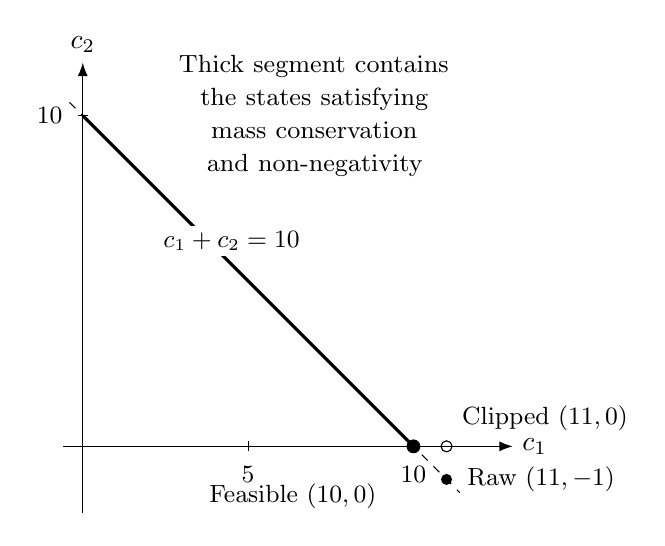
\begin{tikzpicture}[x=0.42cm,y=0.42cm,>=Latex]
\draw[->] (-0.6,0)--(13,0) node[right] {$c_1$};
\draw[->] (0,-2)--(0,11.6) node[above] {$c_2$};
\draw[dashed] (-0.4,10.4)--(11.4,-1.4);
\draw[very thick] (0,10)--(10,0);
\foreach \x in {5,10} {\draw (\x,0.15)--(\x,-0.15) node[below=2pt] {\small\x};}
\draw (0.15,10)--(-0.15,10) node[left=2pt] {\small 10};
\fill (11,-1) circle (2pt) node[right=4pt] {\small Raw $(11,-1)$};
\draw (11,0) circle (2pt) node[above right=3pt] {\small Clipped $(11,0)$};
\fill (10,0) circle (2.5pt);
\node[below left=14pt] at (10,0) {\small Feasible $(10,0)$};
\node[fill=white,inner sep=2pt] at (4.5,6.2) {\small $c_1+c_2=10$};
\node[align=center,text width=4cm] at (7,10) {\small Thick segment contains the states satisfying mass conservation and non-negativity};
\end{tikzpicture}
\caption{Hypothetical two-component geometry showing why clipping a negative concentration can violate a sum fixed by mass conservation.}
\label{fig:assessment_feasible_segment}
\end{figure}

The raw point lies on the extended mass-conservation line but below the concentration boundary. The clipped point enters the non-negative region but leaves the conservation line. The jointly feasible point lies on the thick segment satisfying both conditions. The geometry therefore makes clear why the two requirements must be evaluated on the same returned state.

Marginal compliance summaries can also conceal joint failure. Suppose one prediction satisfies mass conservation but violates non-negativity, while another satisfies non-negativity but violates mass conservation. The marginal compliance frequency of each condition is one half, yet neither state is jointly feasible. The joint feasible frequency is therefore zero. This distinction motivates the use of a state-level indicator that checks both requirements before counting a prediction as physically admissible.

\subsection{The Kircher--Votsmeier projection for mass conservation and non-negativity}

\subsubsection{A positive provisional target and relative-error geometry}

\citet{KircherVotsmeier2025} develop a projection that combines mass conservation and non-negativity for mechanistic-kinetics surrogates. Its application here uses the invariant operator $A$, the null-space basis $Z$, and the feasible influent state as an anchor. Importantly, the procedure operates on the completed component prediction rather than on the internal architecture of the learner. The same projection can therefore be applied to every comparator without altering how that comparator is trained.

The first step replaces any raw component at or below a small positive floor by that floor. For component $j$,
\[
c_{+,ij}^{(m)}=\max(c_{raw,ij}^{(m)},\varepsilon_{c,j}).
\]
For example, a hypothetical raw pair $(-0.2,3)$ becomes $(10^{-8},3)$ when both component floors equal $10^{-8}$ in their native units. The positive floor ensures that every component can be used as a denominator in the weighting that follows.

A diagonal weight matrix then places the reciprocal of each provisional concentration on its diagonal. For a hypothetical positive pair $(1,2)^\top$,
\[
W=\begin{bmatrix}1&0\\0&1/2\end{bmatrix},\qquad
Wh=\begin{bmatrix}h_1\\h_2/2\end{bmatrix}.
\]
The operation does not mix components. Instead, it divides each discrepancy by that component's own provisional concentration. The projection therefore measures movement in relative rather than absolute terms. In compact form,
\begin{equation}
\equationname{Positive provisional target and relative projection weights}
c_{+,i}^{(m)}=\max(c_{raw,i}^{(m)},\boldsymbol{\varepsilon}_c),\qquad
W_i^{(m)}=\operatorname{Diag}\bigl(\mathbf{1}\oslash c_{+,i}^{(m)}\bigr).
\label{eq:projection_positive_target}
\end{equation}
The maximum and division are componentwise, and every entry of $\boldsymbol{\varepsilon}_c$ is $10^{-8}$ in the native unit of that component.

The provisional target serves two purposes: it gives the mass-conservation solve a strictly positive reference state, and it defines the relative-error weights. For a component change $h_j$, the weighted discrepancy is
$h_j/c_{+,ij}^{(m)}$.
A movement of 1 g m$^{-3}$ therefore has relative size 0.01 when the provisional concentration is 100 g m$^{-3}$, but relative size 10 when the provisional concentration is 0.1 g m$^{-3}$. Small component values are consequently protected more strongly against absolute movement, while large components can absorb larger absolute adjustments at the same relative cost. This geometry differs from the training-standardized error metric used later for accuracy assessment \citep{KircherVotsmeier2025,SturmSilva2024}.

\subsubsection{Selecting a candidate that satisfies mass conservation}

The invariant structure from Chapter~\ref{ch:foundations} provides a convenient parameterization of every state that preserves the influent mass-conservation target. If $Z$ contains fifteen basis vectors spanning the allowable component changes, then any mass-conserving state can be written as
\begin{equation}
\equationname{Null-space parameterization of states satisfying mass conservation}
c=c_{in,i}+Zq,\qquad q\in\mathbb{R}^{15}.
\label{eq:projection_affine_parameterization}
\end{equation}
Because $AZ=0$, any vector $Zq$ changes the component state without changing the invariant inventory.

A two-component example shows how the projection coordinates are chosen. Suppose the required sum is four, the feasible influent anchor is $(2,2)^\top$, and the provisional target is $(1,2)^\top$. The provisional target sums to three and therefore violates the required equality. Define
\[
A_{\rm ex}=\frac1{\sqrt2}\begin{bmatrix}1&1\end{bmatrix},\qquad
Z_{\rm ex}=\frac1{\sqrt2}\begin{bmatrix}1\\-1\end{bmatrix}.
\]
These satisfy $A_{\rm ex}Z_{\rm ex}=0$. A scalar movement $t$ produces the candidate
$(2+t,2-t)^\top$, whose sum remains four for every $t$. In the normalized basis, the corresponding null-space coordinate is $q=\sqrt2t$.

The provisional change from the anchor is $(-1,0)^\top$. The difference between an allowable change and this target is therefore $(t+1,-t)^\top$. The inverse provisional concentrations are 1 and $1/2$, so the weighted discrepancy becomes $(t+1,-t/2)^\top$. Its squared norm is
\[
E(t)=(t+1)^2+\frac{t^2}{4}.
\]
The first term penalizes movement away from the provisional value of the first component, and the second penalizes movement in the second component relative to its larger provisional concentration.

Differentiating gives
\[
\frac{dE}{dt}=2(t+1)+\frac t2=\frac52t+2.
\]
Setting the derivative to zero gives $t=-4/5$. Since the second derivative is $5/2>0$, this point is the unique minimum. The resulting candidate is
\[
(2-4/5,2+4/5)^\top=(6/5,14/5)^\top=(1.2,2.8)^\top.
\]
Its relative discrepancies from the provisional target are 0.2 and 0.4, giving squared objective
$0.2^2+0.4^2=0.20$.
By comparison, the mass-conserving candidate $(1.5,2.5)^\top$ gives
$0.5^2+0.25^2=0.3125$.
The relative weighting therefore favors the first candidate because the smaller provisional component is penalized more strongly for a given absolute movement.

Figure~\ref{fig:relative_projection_geometry} visualizes the same calculation. The ellipses represent equal values of the relative-error objective, while the mass-conservation line restricts the allowable candidate states.

\begin{figure}[htbp]
\centering
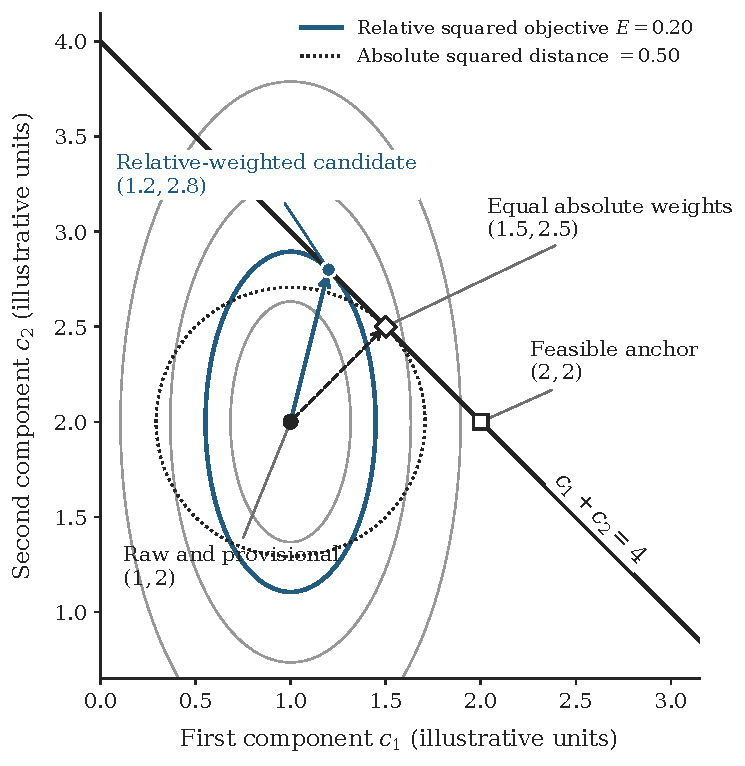
\includegraphics[width=0.79\textwidth]{ch4_concept_weighted_projection.pdf}
\caption{Hypothetical projection for mass conservation with relative and equal absolute weights. The highlighted ellipse first touches the line defined by mass conservation at the relative-weighted candidate. The dotted circle touches it at the equal-absolute-weight candidate.}
\label{fig:relative_projection_geometry}
\end{figure}

The relative-weighted ellipse is elongated because movement in the second component is divided by two. A larger absolute change in that component can therefore have the same weighted cost as a smaller change in the first. An equal-absolute-weight geometry would instead produce circular contours. Both candidate points satisfy the same mass-conservation equality; the difference lies in the metric used to choose among them. The influent state supplies the feasible anchor from which all mass-conserving changes are constructed, but it need not be the closest point to the provisional target.

For the full twenty-component problem, define
$d_j=c_{+,ij}^{(m)}-c_{in,ij}$ and
$w_j=1/c_{+,ij}^{(m)}$.
The projection objective becomes
\[
E(q)=\sum_{j=1}^{20}
w_j^2\left(\sum_{k=1}^{15}Z_{jk}q_k-d_j\right)^2.
\]
For each component, the inner sum forms the allowable mass-conserving change, subtracting $d_j$ gives the discrepancy from the provisional target change, and multiplication by $w_j^2$ converts that discrepancy to the adopted relative scale. Summation over the twenty components gives the complete objective.

The selected coordinates are therefore
\begin{equation}
\equationname{Weighted least-squares problem for projection coordinates}
q_i^{*,(m)}=\underset{q\in\mathbb{R}^{15}}{\operatorname{argmin}}
\left\|W_i^{(m)}\bigl[Zq-(c_{+,i}^{(m)}-c_{in,i})\bigr]\right\|_2^2.
\label{eq:projection_weighted_least_squares}
\end{equation}
The notation $\operatorname{argmin}$ identifies the coordinate vector that minimizes the objective rather than the minimum objective value itself.

Because the objective is quadratic, its stationary conditions are obtained by differentiating with respect to each coordinate $q_\ell$. The derivative is
\[
\frac{\partial E}{\partial q_\ell}
=2\sum_{j=1}^{20}w_j^2 Z_{j\ell}
\left(\sum_{k=1}^{15}Z_{jk}q_k-d_j\right).
\]
Setting these derivatives to zero gives
\[
\sum_{k=1}^{15}\left(\sum_{j=1}^{20}w_j^2Z_{j\ell}Z_{jk}\right)q_k
=\sum_{j=1}^{20}w_j^2Z_{j\ell}d_j,
\]
which collects into the normal equations
\begin{equation}
\equationname{Normal equations for weighted projection coordinates}
Z^\top(W_i^{(m)})^2Zq_i^{*,(m)}
=Z^\top(W_i^{(m)})^2(c_{+,i}^{(m)}-c_{in,i}).
\label{eq:projection_normal_conditions}
\end{equation}

For the hypothetical two-component example,
$Z_{\rm ex}^\top W^2Z_{\rm ex}=(1+1/4)/2=5/8$,
while the right-hand side is $-1/\sqrt2$. Solving gives
$q^*=-8/(5\sqrt2)=-4\sqrt2/5$, which is exactly $\sqrt2t$ for the scalar optimum derived above. The scalar and matrix calculations therefore describe the same projection.

The minimizer is unique. For any nonzero vector $v$,
\[
v^\top Z^\top(W_i^{(m)})^2Zv
=
\|W_i^{(m)}Zv\|_2^2.
\]
Because $Z$ has independent columns and $W_i^{(m)}$ has strictly positive diagonal entries, this quantity is positive whenever $v\neq0$. The coefficient matrix is therefore positive definite.

The selected coordinates define the mass-conserving candidate
\begin{equation}
\equationname{Component candidate satisfying mass conservation}
c_{cand,i}^{(m)}=c_{in,i}+Zq_i^{*,(m)}.
\label{eq:projection_conservative_candidate}
\end{equation}
In the two-component example,
$(2,2)^\top+(-0.8,0.8)^\top=(1.2,2.8)^\top$.
The candidate is non-negative and satisfies the same invariant value as the anchor. Because $AZ=0$,
\[
Ac_{cand,i}^{(m)}=Ac_{in,i}=b_i
\]
in exact arithmetic. If the provisional target is already mass-conserving, its change lies in the null space of $A$ and the least-squares residual can be zero, so the candidate reproduces the provisional target to numerical tolerance.

Equation~\eqref{eq:projection_normal_conditions} provides the analytical stationary condition but is not used through an explicit matrix inverse. Numerically, the weighted design $W_i^{(m)}Z$ is solved using an orthogonal--triangular factorization, with singular-value decomposition and relative cutoff $10^{-12}$ as a fallback. Near-zero provisional concentrations can produce highly unequal weights. Solving the original weighted system avoids the additional conditioning penalty associated with forming and explicitly inverting the normal-equation matrix \citep{BuzziFerraris2013}.

\subsubsection{The largest feasible interpolation toward the candidate}

The mass-conserving candidate can still contain a negative component. When this occurs, the projection does not alter individual coordinates independently. Instead, it shortens the complete mass-conserving direction from the feasible influent anchor toward the candidate.

Consider a three-component example with total inventory fixed at 10. Let the feasible influent be
$(8,1,1)^\top$
and let the mass-conserving candidate be
$(4,-0.5,6.5)^\top$.
Their difference is
$(-4,-1.5,5.5)^\top$.
A fraction $\alpha$ of this direction gives
\[
c_1(\alpha)=8-4\alpha,\qquad
c_2(\alpha)=1-1.5\alpha,\qquad
c_3(\alpha)=1+5.5\alpha.
\]
The first component requires $\alpha\leq2$, the second requires $\alpha\leq2/3$, and the third imposes no upper bound for $\alpha\geq0$. Because the interpolation is restricted to $0\leq\alpha\leq1$, the second component reaches the non-negative boundary first at $\alpha=2/3$.

For the general problem, define the candidate direction
\begin{equation}
\equationname{Candidate direction from the feasible influent anchor}
\delta_i^{(m)}=c_{cand,i}^{(m)}-c_{in,i}=Zq_i^{*,(m)}.
\label{eq:projection_candidate_direction}
\end{equation}
Every point
$c_{in,i}+\alpha\delta_i^{(m)}$
with $0\leq\alpha\leq1$ remains mass-conserving because
$A\delta_i^{(m)}=0$.

For a decreasing coordinate,
\[
c_{in,ij}+\alpha\delta_{ij}^{(m)}\geq0.
\]
When $\delta_{ij}^{(m)}<0$, rearrangement gives
\begin{equation}
\equationname{Interpolation bound for a decreasing concentration}
\alpha\leq\frac{c_{in,ij}}{-\delta_{ij}^{(m)}}
\qquad\text{when }\delta_{ij}^{(m)}<0.
\label{eq:projection_coordinate_bound}
\end{equation}
The smallest of these ratios identifies the first non-negativity boundary encountered along the segment.

If the candidate is already non-negative, the full direction is retained and $\alpha=1$. Otherwise, the smallest admissible ratio is reduced slightly by a numerical safety factor $1-\eta$, with $\eta=10^{-12}$, to limit sign changes from finite-precision arithmetic. The interpolation factor and returned state are
\begin{equation}
\equationname{Interpolation factor and final state satisfying non-negativity}
\begin{split}
\alpha_i^{(m)}&=
\begin{cases}
1, & c_{cand,i}^{(m)}\geq0,\\
(1-\eta)\displaystyle\min_{j\,\mid\,\delta_{ij}^{(m)}<0}
\frac{c_{in,ij}}{-\delta_{ij}^{(m)}}, & \text{otherwise},
\end{cases}\\
\tilde c_i^{(m)}&=c_{in,i}+\alpha_i^{(m)}\delta_i^{(m)}.
\end{split}
\label{eq:projection_positivity_backtracking}
\end{equation}
The factor is restricted to $[0,1]$ against roundoff.

Because the influent state is non-negative, the interpolation remains in the non-negative orthant. Decreasing coordinates satisfy
$\tilde c_{ij}^{(m)}\geq\eta c_{in,ij}\geq0$,
and increasing coordinates remain non-negative automatically. Mass conservation is also retained:
\begin{equation}
\equationname{Mass conservation identity for the final projected state}
A\tilde c_i^{(m)}=Ac_{in,i}+\alpha_i^{(m)}AZq_i^{*,(m)}=b_i.
\label{eq:projection_final_conservation}
\end{equation}
Thus one scalar interpolation preserves the complete mass-conserving direction while moving the state back to the non-negative region.

Returning to the three-component example, the decreasing-coordinate bounds are 2 and $2/3$, so the largest feasible factor is $2/3$. Ignoring the numerical safety margin for illustration,
\[
(8,1,1)^\top+\frac23(-4,-1.5,5.5)^\top
=
(16/3,0,14/3)^\top.
\]
The total remains 10 and all components are non-negative. The first component changes even though the second component is the one that reaches the boundary. This is an important consequence of shortening the complete direction rather than clipping a single coordinate.

If an influent component is zero and the candidate direction decreases that same coordinate, its bound is zero and the final state returns to the influent anchor. This is still feasible. Similarly, a component absent from the invariant rows can nevertheless move when the entire direction is shortened. For that reason, the interpolation factor and its activation frequency are retained as projection diagnostics.

\subsubsection{Numerical acceptance and returned predictions}

The algebra above establishes the desired properties in exact arithmetic. The numerical implementation still requires explicit checks on the returned state.

For invariant row $h$, define
\[
r_h=\sum_jA_{hj}\tilde c_{ij}^{(m)}-b_{ih}.
\]
The five residuals are combined through their Euclidean norm. Non-negativity is assessed separately against a component-specific numerical tolerance. For example, a concentration of $-5\times10^{-11}$ passes a tolerance of $10^{-10}$, whereas $-2\times10^{-10}$ does not. A projected state is accepted only when
\begin{equation}
\equationname{Numerical mass conservation and non-negativity acceptance checks}
\|A\tilde c_i^{(m)}-b_i\|_2\leq\tau_{mc},\qquad
\tilde c_{ij}^{(m)}\geq-\tau_{nn,j}\quad\text{for every }j,
\label{eq:projection_numerical_acceptance}
\end{equation}
with $\tau_{mc}=10^{-10}$ in the fixed invariant-coordinate convention and
$\tau_{nn,j}=10^{-10}$ in the native unit of component $j$. A finite raw prediction is required before projection begins.

The final state therefore satisfies the declared invariant and sign requirements to the stated numerical tolerances. The least-squares stage minimizes relative movement within the affine mass-conservation set. The interpolation stage, when needed, selects a point on the line segment between the feasible influent and the mass-conserving candidate. These operations have a different objective from the later prediction-error calculation, which is standardized using training-response variability.

Figure~\ref{fig:projection_acceptance_flow} summarizes the complete procedure.

\begin{figure}[htbp]
\centering
\begingroup
\linespread{1}\selectfont
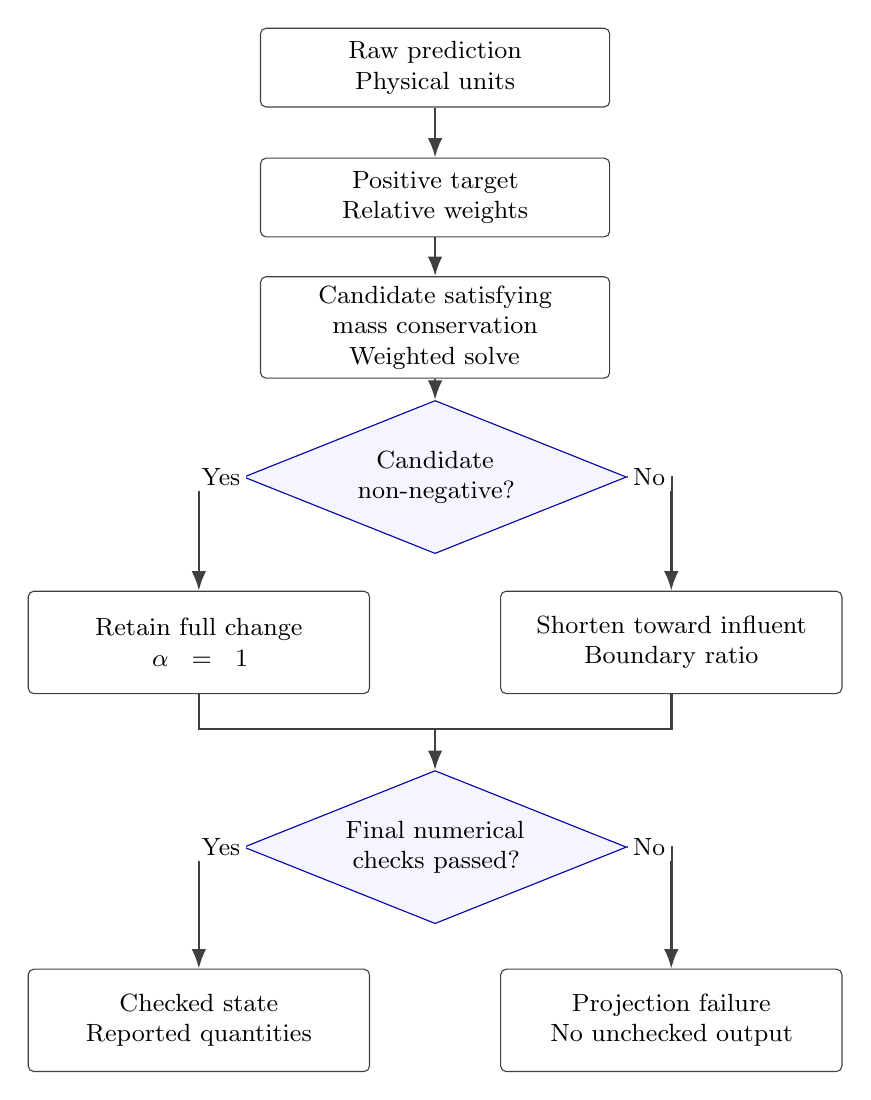
\begin{tikzpicture}[
    >=Latex,
    block/.style={draw=black!75,fill=white,rounded corners=2pt,
        text width=4.2cm,minimum height=1cm,align=center,font=\small},
    branch/.style={draw=black!75,fill=white,rounded corners=2pt,
        text width=4.1cm,minimum height=1.3cm,align=center,font=\small},
    test/.style={diamond,draw=blue!65!black,fill=blue!4,aspect=2.5,
        text width=2.7cm,align=center,inner sep=2pt,font=\small},
    flow/.style={->,line width=.9pt,draw=black!75},
    tag/.style={font=\small,fill=white,inner sep=2pt}]
\node[block] (raw) at (0,0) {Raw prediction\\Physical units};
\node[block] (positive) at (0,-1.65) {Positive target\\Relative weights};
\node[block] (candidate) at (0,-3.3) {Candidate satisfying mass conservation\\Weighted solve};
\node[test] (non-negative) at (0,-5.2) {Candidate\\non-negative?};
\node[branch] (full) at (-3.0,-7.3) {Retain full change\\$\alpha=1$};
\node[branch] (shorten) at (3.0,-7.3) {Shorten toward influent\\Boundary ratio};
\coordinate (join) at (0,-8.4);
\node[test] (audit) at (0,-9.9) {Final numerical\\checks passed?};
\node[branch] (return) at (-3.0,-12.1) {Checked state\\Reported quantities};
\node[branch] (failure) at (3.0,-12.1) {Projection failure\\No unchecked output};
\draw[flow] (raw)--(positive);
\draw[flow] (positive)--(candidate);
\draw[flow] (candidate)--(non-negative);
\draw[flow] (non-negative.west)-|(full.north) node[pos=.25,tag] {Yes};
\draw[flow] (non-negative.east)-|(shorten.north) node[pos=.25,tag] {No};
\draw[draw=black!75,line width=.9pt] (full.south)|-(join);
\draw[draw=black!75,line width=.9pt] (shorten.south)|-(join);
\draw[flow] (join)--(audit.north);
\draw[flow] (audit.west)-|(return.north) node[pos=.25,tag] {Yes};
\draw[flow] (audit.east)-|(failure.north) node[pos=.25,tag] {No};
\end{tikzpicture}
\endgroup

\caption{Post prediction mass conservation and non-negativity procedure. Positive-target construction, projection for mass conservation, and final-state acceptance have separate roles. The diagram shows the sequence used for each prediction.}
\label{fig:projection_acceptance_flow}
\end{figure}

The provisional positive target defines the relative weights used by the mass-conservation solve. If the resulting candidate is non-negative, the complete mass-conserving change is retained. If the candidate crosses a concentration boundary, the direction is shortened from the feasible influent anchor. Both branches end in the same numerical audit, so every returned projected state is judged by identical mass-conservation and non-negativity criteria.

COD, TN, TP, and TSS are calculated only after the component state has been produced. The same reporting map is used for raw and projected predictions:
\begin{equation}
\equationname{Raw and projected water-quality composites}
y_{raw,i}^{(m)}=I_{comp}c_{raw,i}^{(m)},\qquad
\tilde y_i^{(m)}=I_{comp}\tilde c_i^{(m)}.
\label{eq:projection_paired_composites}
\end{equation}
A paired composite comparison therefore changes only the component state supplied to the fixed reporting map. Physical feasibility is assessed before this aggregation, on the complete twenty-component state itself.

\section{Methodology}

\subsection{Constructing a mechanistic learning domain}

The reactor benchmark was designed around 10,000 accepted steady-state cases. Each candidate varies all twenty-two surrogate inputs: HRT, aeration, and the twenty influent component concentrations.

A randomized, scrambled, strength-one Latin hypercube was generated with seed 42. For each input coordinate, the method places one sample in each marginal stratum before the unit-hypercube design is linearly mapped to the physical bounds in Table~\ref{tab:reactor_sampling_domain}. No subsequent design optimization was applied. This sampling strategy distributes cases across each declared marginal range without requiring the exponential number of combinations that would arise from a full Cartesian grid \citep{McKay1979}.

\begin{table}[htbp]
\centering\small
\caption{Design bounds for the standalone reactor learning domain. The intervals define the sampled input ranges.}\label{tab:reactor_sampling_domain}
\begin{tabular}{lp{5.7cm}ll}
\toprule
Input & Meaning & Interval & Unit\\
\midrule
HRT & Hydraulic operating input & $[6,36]$ & h\\
$u_{\mathrm{air}}$ & Dimensionless aeration input & $[0.5,2.5]$ & 1\\
$S_O$ & Influent dissolved oxygen & $[0,0.5]$ & g O$_2$ m$^{-3}$\\
$S_F$ & Influent fermentable substrate & $[20,180]$ & g COD m$^{-3}$\\
$S_A$ & Influent acetate & $[5,80]$ & g COD m$^{-3}$\\
$S_{NH4}$ & Influent ammonium nitrogen & $[12,55]$ & g N m$^{-3}$\\
$S_{NO2}$ & Influent nitrite nitrogen & $[0,3]$ & g N m$^{-3}$\\
$S_{NO3}$ & Influent nitrate nitrogen & $[0,8]$ & g N m$^{-3}$\\
$S_{N2}$ & Influent dissolved dinitrogen & $[0,2]$ & g N m$^{-3}$\\
$S_{PO4}$ & Influent soluble phosphate & $[2,18]$ & g P m$^{-3}$\\
$S_I$ & Influent soluble inert organic matter & $[10,90]$ & g COD m$^{-3}$\\
$S_{ALK}$ & Influent alkalinity & $[80,260]$ & mol m$^{-3}$\\
$X_I$ & Influent particulate inert matter & $[20,120]$ & g COD m$^{-3}$\\
$X_S$ & Influent slowly biodegradable substrate & $[60,280]$ & g COD m$^{-3}$\\
$X_H$ & Influent heterotrophic biomass & $[15,100]$ & g COD m$^{-3}$\\
$X_{PAO}$ & Influent phosphate-accumulating biomass & $[5,60]$ & g COD m$^{-3}$\\
$X_{PP}$ & Influent stored polyphosphate & $[2,20]$ & g P m$^{-3}$\\
$X_{PHA}$ & Influent stored polyhydroxyalkanoates & $[1,30]$ & g COD m$^{-3}$\\
$X_{AOB}$ & Influent ammonia-oxidizing biomass & $[0.5,8]$ & g COD m$^{-3}$\\
$X_{NOB}$ & Influent nitrite-oxidizing biomass & $[0.5,8]$ & g COD m$^{-3}$\\
$X_{MeP}$ & Influent precipitated metal phosphate & $[0,12]$ & g TSS m$^{-3}$\\
$X_{MeOH}$ & Influent metal hydroxide & $[0,12]$ & g TSS m$^{-3}$\\
\bottomrule
\end{tabular}
\end{table}

The standalone reactor domain uses only the operating and influent bounds declared in this table. Its alkalinity interval remains in the native coordinate used by the mechanistic model. The connected plant study in Chapter~\ref{ch:plant} uses a separate operating domain and separate influent bounds.

For every candidate input, Equation~\eqref{eq:reactor_steady_balance} was solved by nonlinear least squares. Each component concentration was bounded numerically to $[10^{-8},1500]$ in its native unit. The cost-change, step-size, and gradient convergence tolerances were all $10^{-9}$, with at most 1200 function evaluations per steady-state solve. The overall generation procedure allowed up to 25 attempted candidates for every target retained state.

A candidate was retained only when the numerical solver converged and the maximum absolute component-balance residual was no greater than $10^{-9}$ in the fixed native component-unit-per-day coordinates. The acceptance criterion therefore refers directly to the steady-state balance equations rather than to the later invariant residual.

Two physically informed initial states were attempted before dynamic relaxation. The first blended the sampled influent with the preceding accepted effluent when such a state was available. It reduced readily consumed substrate concentrations, retained biomass pools, and estimated dissolved oxygen from dilution and transfer. The second imposed stronger substrate depletion and biomass enrichment. Both initial-state vectors were restricted to $[10^{-6},1500]$.

If both steady-state solves failed, the dynamic balance was integrated for 20 days with a stiff backward differentiation formula, and the resulting state was used as a new initial condition for the steady solve. The concentration bounds and initial-state restrictions applied to the state variables only. The 28 kinetic process rates were evaluated without artificial clipping or an imposed rate ceiling.

Several diagnostics were retained separately: solver acceptance, invariant residual, and minimum concentration. This separation is important because one numerical success does not guarantee the others. A bounded least-squares solve can terminate without meeting the required steady-state residual. A strictly positive state can still violate a mass-conservation invariant. Conversely, a state can have a small invariant residual without satisfying the component-balance acceptance criterion used for mechanistic generation. The surrogate inputs therefore contain only the sampled operating and influent coordinates; initialization choices and solver history are not supplied as predictive features.

\subsection{Preprocessing and validation without response leakage}

The model comparison uses nested cross-validation so that hyperparameter selection and final assessment remain separated. A fold is one reserved subset of cases. In the outer loop, each fold is withheld in turn for model assessment. Within the corresponding outer-training pool, an inner cross-validation loop is used for hyperparameter selection.

Learning behavior is evaluated at eleven nested design sizes,
\begin{equation}
\equationname{Observation counts for nested reactor assessment}
N\in\{500,1450,2400,3350,4300,5250,6200,7150,8100,9050,10000\}.
\label{eq:reactor_nested_sample_sizes}
\end{equation}
A seed-42 permutation fixes the row order and the master outer-fold identifiers before any subset is formed. Smaller datasets are therefore true subsets of the larger ones, and each row retains the same outer-fold assignment whenever it appears. This design allows the learning curves to reflect changing data availability without simultaneously changing the underlying fold structure.

Five outer folds are used. At each design size, four folds provide $0.8N$ training cases and the remaining fold provides $0.2N$ assessment cases. Thus, $N=500$ gives 400 training cases and 100 scored cases per outer iteration, while $N=10{,}000$ gives 8000 training cases and 2000 scored cases. Across the five outer iterations, every row is scored exactly once by a model whose fit excluded that row. All thirteen surrogates use the same rows and fold identities, and raw and projected predictions are compared on those same observations.

Hyperparameter selection occurs only inside the outer-training data. Four inner folds are constructed within the largest outer-training partition. For an 8000-row outer-training pool, an inner iteration therefore fits on 6000 rows and validates on the remaining 2000 rows from that pool. These inner-validation cases are distinct from the 2000 cases reserved for the outer assessment. After the best setting is selected, the model is refitted on the applicable outer-training subset and scored on the withheld outer fold.

For each outer fold, the setting selected at the largest design size is retained when that same fold is evaluated at the smaller nested sizes. The resulting learning curve therefore measures the response to sample size under a fixed fold-specific setting rather than repeatedly retuning the model at every point. This distinction is relevant because prediction error need not change monotonically with either model capacity or data availability \citep{Belkin2019}. The learning-curve framework of \citet{VieringLoog2023} further motivates interpreting the complete trajectory rather than only its endpoint.

Every transformation is estimated from the training partition applicable to the fit. During inner selection, this is the inner-training split. During outer assessment, it is the outer-training subset at the current size. During extrapolation assessment, it is the complete 10,000-case in-domain training pool.

For a training coordinate with values $v_1,\ldots,v_M$, the mean and population standard deviation are
\[
\mu=\frac{v_1+\cdots+v_M}{M},\qquad
\sigma^2=\frac{(v_1-\mu)^2+\cdots+(v_M-\mu)^2}{M},\qquad
\sigma=\sqrt{\sigma^2}.
\]
The population variance divides by the training count $M$. A standardized value is then
$z=(v-\mu)/\sigma$, requiring $\sigma>0$.

For example, training values 2, 2, 6, and 6 have mean 4 and population standard deviation 2. A validation value of 6 is therefore transformed to
$(6-4)/2=1$.
The validation value does not contribute to the training mean or variance. If the standardized coordinate is a target and a model predicts 0.5, the inverse transformation gives
$4+2(0.5)=5$
in the target's physical unit.

Each target component has its own training mean and standard deviation. Consequently, target-scaled predictions are transformed back component by component before projection or physical diagnostics. Using one common inverse scale across components would be incorrect because the component concentrations differ in both units and variability.

\begin{table}[htbp]
\centering
\caption{Output handling and preprocessing for the statistical comparators. Scaling uses only the training partition applicable to each fit.}
\label{tab:surrogate_preprocessing}
\small
\begin{tabular}{p{5.1cm}p{3.2cm}p{3.3cm}}
\toprule
Surrogates & Output handling & Scaling\\
\midrule
XGBoost, LightGBM, CatBoost & Separate component regressors & None\\
AdaBoost & Separate component regressors & Targets only\\
Random Forest & Joint tree response & None\\
Extra Trees & Joint tree response & Targets only\\
Support vector regression & Separate component regressors & Inputs and targets\\
$k$-nearest neighbors & Joint neighborhood response & Inputs and targets\\
Partial least squares, Multi-task Lasso, Multi-task Elastic Net & Joint coefficient structure & Inputs and targets\\
Multilayer perceptron, TabNet & Joint neural output & Inputs and targets\\
\bottomrule
\end{tabular}
\end{table}

The preprocessing choices reflect the numerical structure of each learner. Positive affine rescaling of a single input coordinate preserves the ordering used by tree threshold partitions. Distance-based, covariance-based, and coefficient-regularized methods are more sensitive to coordinate magnitude because their objectives directly combine numerical differences across inputs. Separate-output tree regressors likewise do not combine differently scaled target components in one joint fitting loss.

The target-only scaling retained for Extra Trees and AdaBoost is a specified benchmark choice. Regardless of these training decisions, all final component errors are placed on a common assessment scale defined from the applicable training response. Training-time scaling and evaluation-time normalization therefore serve different purposes.

No missing-value imputation, response-based outlier removal, or target filtering was applied. Validation and extrapolation responses were never used to estimate a preprocessing quantity. Standardizing a validation target using the variance of the validation fold itself would alter the scoring reference using information unavailable during training. The present procedure instead asks how large a prediction error is relative to the response variability that the fitted learner was permitted to observe.

\subsection{Hyperparameter selection}

Hyperparameters were selected using a seeded tree-structured Parzen estimator search. Each study used 100 trials, with no pruning and no timeout. A trial proposed one complete parameter setting, fitted that setting within the prescribed inner-training partitions, and evaluated the resulting validation objective. The objective was the mean squared standardized component error and was minimized. It is therefore distinct from any individual hyperparameter such as tree depth, learning rate, or penalty strength.

The search procedure follows the optimization framework of \citet{Akiba2019}. Five independent studies selected settings for the five largest-scale outer-training partitions. A sixth four-fold study selected the setting used for the final full-domain refit. Thus, each surrogate required
$6(100)=600$
trials, and all thirteen surrogates required
$13(600)=7800$
trials under the declared protocol.

\begin{table}[htbp]
\centering\small
\caption{Search domains and fixed controls for tree ensemble surrogates. Integer limits are inclusive. ``Log'' denotes a log-uniform search.}\label{tab:surrogate_search_domains}
\begin{tabular}{p{2.65cm}p{9.2cm}}
\toprule
Surrogate & Search domain and fixed controls\\
\midrule
XGBoost & 80--320 trees. Learning rate 0.01--0.2 (log). Depth 3--8. Minimum child weight 0.5--8 (log). Row and feature fractions 0.6--1. Absolute-value penalty $10^{-6}$--1 (log). Squared penalty $10^{-3}$--10 (log). Histogram or approximate trees. Squared-error objective.\\
LightGBM & 80--320 trees. Learning rate 0.01--0.2 (log). 15--63 leaves. Depth unbounded or in $\{4,6,8,10\}$. Minimum child rows 5--40. Row and feature fractions 0.6--1 with subsampling frequency 1. Absolute-value penalty $10^{-6}$--1 (log). Squared penalty $10^{-6}$--10 (log). Regression objective.\\
CatBoost & 80--320 iterations. Learning rate 0.01--0.2 (log). Depth 4--8. Squared penalty 0.01--20 (log). Bagging temperature 0--5. Random strength $10^{-3}$--5 (log). Root mean squared error loss and Bayesian bootstrap.\\
AdaBoost & 50--250 depth-three trees. Learning rate 0.01--1 (log). Linear, squared, or exponential regression loss.\\
Random Forest & 100--400 trees. Depth unbounded or in $\{6,10,14,18\}$. Minimum split size 2--10. Minimum leaf size 1--4. Feature fraction 0.5--1. Bootstrap enabled or disabled.\\
Extra Trees & 100--400 trees. Depth unbounded or in $\{6,10,14,18\}$. Minimum split size 2--10. Minimum leaf size 1--4. Feature fraction 0.5--1. Bootstrap enabled or disabled.\\
\bottomrule
\end{tabular}
\end{table}

\begin{table}[htbp]
\centering\small
\caption{Search domains and fixed controls for kernel, neighbor, multiresponse, and neural surrogates. Integer limits are inclusive. ``Log'' denotes a log-uniform search.}\label{tab:surrogate_search_domains_other}
\begin{tabular}{p{2.65cm}p{9.2cm}}
\toprule
Surrogate & Search domain and fixed controls\\
\midrule
Support vector regression & Penalty 0.1--10 (log). Error-insensitive width 0.01--0.5 (log). Linear or radial kernel. Radial coefficient set from standardized input variance or inverse input dimension. Tolerance $10^{-3}$--$10^{-2}$ (log). Shrinking enabled. At most 20,000 iterations. Kernel cache of 256 megabytes per output regressor.\\
$k$-nearest neighbors & 1--15 neighbors. Uniform or distance weights. Automatic, ball-tree, $k$-dimensional tree, or brute-force search. Leaf size 15--60. Minkowski, Euclidean, or Manhattan distance. Minkowski order in $\{1,2,3\}$.\\
Partial least squares & 1--6 latent components. 200--1000 maximum iterations. Tolerance $10^{-8}$--$10^{-4}$ (log). Internal scaling disabled because external training-partition scaling is applied.\\
Multi-task Elastic Net & Penalty strength $10^{-6}$--10 (log). Row-group mixing ratio 0.05--0.95. Cyclic coordinate descent. At most 20,000 iterations and tolerance $10^{-6}$.\\
Multi-task Lasso & Penalty strength $10^{-6}$--10 (log). Cyclic coordinate descent. At most 20,000 iterations and tolerance $10^{-6}$.\\
Multilayer perceptron & Hidden widths $(128,64,32)$. Rectified linear, hyperbolic tangent, or logistic activation. Adaptive moment optimization. Squared-weight penalty $10^{-6}$--$10^{-2}$ (log). Batch size in $\{64,128,256\}$. Learning rate $5\times10^{-4}$--$10^{-2}$ (log). Training-loss tolerance $10^{-4}$--$10^{-3}$ (log). Shuffling enabled. Training-loss patience 15 epochs. At most 250 epochs.\\
TabNet & Equal decision and attention widths in $\{8,16,24\}$. Three or four attention steps. Relaxation coefficient 1--2. Sparsity coefficient $10^{-6}$--$10^{-2}$ (log). Adaptive moment learning rate 0.003--0.03 (log). Sparsemax or entmax-1.5 masks. 20--50 selected epochs. Batch size in $\{512,1024\}$. Virtual batch size 128. Patience zero.\\
\bottomrule
\end{tabular}
\end{table}

Together, the declared search ranges, fixed controls, and equal trial allocation provide a common fitting protocol for all thirteen predictors.

\subsection{Evaluation of error, feasibility, and projection size}

\subsubsection{Component errors on a training-defined scale}

The primary prediction target is the twenty-component effluent state. Because these coordinates differ in units and variability, the assessment first standardizes each component error using variability estimated only from the applicable training reference.

Let $\mathcal{T}$ denote that training reference, and let
$\sigma_j^{(\mathcal{T})}$
be the population standard deviation of component $j$ within it. For prediction type $t$, either raw or projected, the standardized error is
\begin{equation}
\equationname{Component error standardized by the training response scale}
\xi_{ij}^{(m,t)}=
\frac{c_{ij}^{(m,t)}-c_{out,ij}}{\sigma_j^{(\mathcal{T})}}.
\label{eq:projection_standardized_error}
\end{equation}
A prediction of 3 g N m$^{-3}$ against a reference value of 2 g N m$^{-3}$ has physical error 1 g N m$^{-3}$. If the corresponding training standard deviation is 2 g N m$^{-3}$, the standardized error is 0.5.

The aggregate error metrics are built from these standardized component errors. Consider two observations and two components with training standard deviations 2 and 4. Suppose the reference and predicted values are
\[
\begin{array}{c|cc|cc}
&\multicolumn{2}{c|}{\text{Reference}}&\multicolumn{2}{c}{\text{Prediction}}\\
\text{Observation}&\text{Component 1}&\text{Component 2}&\text{Component 1}&\text{Component 2}\\\hline
1&2&4&3&2\\
2&4&8&2&12
\end{array}
\]
The physical errors are 1, $-2$, $-2$, and 4. Dividing each by the corresponding training standard deviation gives
\[
\xi=\begin{bmatrix}1/2&-2/4\\-2/2&4/4\end{bmatrix}
=
\begin{bmatrix}0.5&-0.5\\-1&1\end{bmatrix}.
\]
The four squared standardized errors sum to 2.5, giving a mean squared standardized error of
$2.5/4=0.625$
and a root mean squared value of approximately 0.7906. Their absolute values sum to 3, giving a mean absolute standardized error of 0.75.

For the complete twenty-component assessment,
\begin{align}
\equationname{Normalized mean squared component error}
\mathrm{nMSE}_{m,t}&=\frac{1}{20n}\sum_{i=1}^{n}\sum_{j=1}^{20}(\xi_{ij}^{(m,t)})^2,\label{eq:projection_nmse}\\
\equationname{Normalized root mean squared component error}
\mathrm{nRMSE}_{m,t}&=\sqrt{\mathrm{nMSE}_{m,t}},\label{eq:projection_nrmse}\\
\equationname{Normalized mean absolute component error}
\mathrm{nMAE}_{m,t}&=\frac{1}{20n}\sum_{i=1}^{n}\sum_{j=1}^{20}|\xi_{ij}^{(m,t)}|.
\label{eq:projection_nmae}
\end{align}
After standardization, each component--observation pair receives equal numerical weight. nRMSE gives greater emphasis to larger standardized errors, while nMAE provides a complementary measure of average deviation. Both require a positive training standard deviation for every component.

This scaling has an important interpretation. A physical error of 1 g m$^{-3}$ corresponds to standardized magnitude 0.1 when the training standard deviation is 10 g m$^{-3}$, but magnitude 10 when the training standard deviation is 0.1 g m$^{-3}$. The assessment therefore measures error relative to the variability the model was exposed to during training rather than treating the same absolute error as equally important for all components.

The coefficient of determination provides a second view of accuracy. For each component, it compares the model's squared error with the squared error obtained by predicting the scored-partition mean for every observation. For component 1 in the hypothetical example, the scored mean is 3. The constant prediction therefore gives a baseline squared error of
$(2-3)^2+(4-3)^2=2$.
The model gives
$(3-2)^2+(2-4)^2=5$,
so
$R^2=1-5/2=-1.5$.
The negative value indicates that the prediction is worse than the constant baseline on that scored partition.

For component $j$,
\begin{equation}
\equationname{Component and macro-average coefficients of determination}
R_{j,m,t}^2=1-
\frac{\sum_i(c_{ij}^{(m,t)}-c_{out,ij})^2}
{\sum_i(c_{out,ij}-\bar c_{out,j})^2},\qquad
\bar R_{m,t}^2=\frac{1}{20}\sum_{j=1}^{20}R_{j,m,t}^2.
\label{eq:projection_r_squared}
\end{equation}
Here
$\bar c_{out,j}$
is the true mean of component $j$ within the scored partition. This mean is used only for scoring and does not enter model fitting. Consequently, the denominator of $R^2$ uses scored-partition variability, whereas nMSE and nRMSE use a training-defined scale. The two measures are therefore complementary rather than interchangeable.

Aggregation must also be interpreted carefully. Pooled nRMSE is the square root of the mean of all squared standardized component errors. It is not the arithmetic mean of the twenty component-level root errors. If two components have mean squared standardized errors of 1 and 9, for example, their pooled root error is
$\sqrt{(1+9)/2}=\sqrt5$,
whereas the mean of their separate roots is
$(1+3)/2=2$.

Physical-unit errors are retained for the individual components. COD, TN, TP, and TSS are evaluated separately as secondary reported quantities. For each composite, the physical-unit RMSE is calculated across observations and then divided by the training standard deviation of that composite. A physical root error of 5 g COD m$^{-3}$ with a training composite standard deviation of 10 g COD m$^{-3}$ therefore gives a normalized composite root error of 0.5. The composite standard deviations are calculated only after the fixed reporting map has been applied to the training target states.

\subsubsection{Violation frequencies and their magnitudes}

Physical diagnostics distinguish how often a state fails from how severely it fails.

The mass-conservation residual is the Euclidean norm of the five invariant discrepancies,
\[
r_h=\sum_jA_{hj}c_j-b_{ih}.
\]
For example, a two-row residual vector of $(3,4)^\top$ has norm 5. This quantity is evaluated in the fixed invariant-coordinate convention.

Negative concentrations require a different summary because the twenty component coordinates have different physical scales. Each concentration is first divided by its training standard deviation. Positive entries are then replaced by zero, and the absolute values of the remaining negative entries are summed. Thus, standardized values $(-2,1.5,-2)$ become $(-2,0,-2)$ and have total negative magnitude 4. Positive components cannot cancel negative components in this diagnostic.

The two violation magnitudes are
\begin{equation}
\equationname{Mass conservation residual and standardized negative concentration}
v_{mc,i}(c)=\|Ac-b_i\|_2,\qquad
v_{nn,i}^{\mathrm{std}}(c)=
\left\|\min(c\oslash\boldsymbol{\sigma}^{(\mathcal{T})},0)\right\|_1.
\label{eq:projection_violation_magnitudes}
\end{equation}
The minimum is componentwise. The negative magnitude uses training standard deviations only to make violations across differently scaled component coordinates comparable; it does not replace the componentwise native-unit sign check used for acceptance.

Violation frequencies are row-level proportions. The indicator $\mathbb{1}[\cdot]$ equals one when its condition is true and zero otherwise. Suppose four hypothetical states have mass-conservation failure indicators $(1,0,1,0)$ and non-negativity failure indicators $(0,1,1,0)$. Each marginal violation frequency is therefore 0.5. A state with several negative components still contributes only one failure to the non-negativity frequency.

The two marginal frequencies are
\begin{equation}
\equationname{Mass conservation and non-negativity violation frequencies}
\pi_{mc}=
\frac{1}{n}\sum_i\mathbb{1}[v_{mc,i}(c_i)>\tau_{mc}],\qquad
\pi_{nn}=
\frac{1}{n}\sum_i\mathbb{1}[\min_j(c_{ij}+\tau_{nn,j})<0].
\label{eq:projection_violation_rates}
\end{equation}
A state is jointly feasible only when both requirements pass in that same observation:
\begin{equation}
\equationname{Jointly feasible fraction of assessed component states}
\pi_{\mathrm{feasible}}=
\frac{1}{n}\sum_i\mathbb{1}
[v_{mc,i}(c_i)\leq\tau_{mc}\ \text{and}\ 
\min_j(c_{ij}+\tau_{nn,j})\geq0].
\label{eq:projection_feasible_fraction}
\end{equation}
The two marginal violation frequencies are not added, because one state can fail both conditions and would otherwise be counted twice. In the four-state example above, only the fourth state passes both tests, so the joint feasible fraction is one quarter.

Mean, median, and maximum violation magnitudes are retained in addition to the frequencies. This distinction separates incidence from severity. Many states can lie only slightly below zero, producing a high violation frequency but small negative magnitudes. A single strongly negative prediction can instead produce a low frequency but a large maximum magnitude. Physical-unit negative magnitudes are also retained separately for each component.

\subsubsection{Paired accuracy effects and displacement}

Because raw and projected predictions are generated from the same fitted model and scored on the same cases, the effect of projection can be measured directly.

For each outer fold,
\begin{equation}
\equationname{Paired difference in projected and raw prediction error}
\Delta\mathrm{nRMSE}_{m,N,g}=
\mathrm{nRMSE}_{m,\mathrm{projected},N,g}
-\mathrm{nRMSE}_{m,\mathrm{raw},N,g}.
\label{eq:projection_paired_error_difference}
\end{equation}
A negative value means that projection reduced the assessed error; a positive value means that it increased it. For example, raw and projected nRMSE values of 0.40 and 0.35 give a difference of $-0.05$, whereas a projected value of 0.45 gives $+0.05$. Differences are calculated within the paired folds before being summarized. Component-level and composite-level differences are also retained because aggregate improvement can coexist with deterioration in specific outputs.

Projection displacement measures something different: how far the returned projected state moves from its own raw prediction. For sample $i$,
\begin{equation}
\equationname{Standardized component displacement caused by projection}
d_{c,i}^{\mathrm{std},(m)}=
\left\|(\tilde c_i^{(m)}-c_{raw,i}^{(m)})
\oslash\boldsymbol{\sigma}^{(\mathcal{T})}\right\|_2.
\label{eq:projection_standardized_displacement}
\end{equation}
The difference is standardized using the training component standard deviations and then combined through a Euclidean norm.

For the earlier two-component weighted-projection example, the raw state $(1,2)$ becomes $(1.2,2.8)$, giving changes of 0.2 and 0.8. If the illustrative training standard deviations are 0.1 and 0.4, the standardized movements are both 2 and the displacement is
$2\sqrt2$.
The training scale used here differs deliberately from the provisional concentration scale used inside the projection. The former measures movement relative to observed response variability; the latter defines the optimization geometry of the physical adjustment.

A large displacement can remove physical violations while moving the state farther from the mechanistic reference \citep{SturmSilva2024,KircherVotsmeier2025}. Displacement is therefore a measure of adjustment, not accuracy. Mean, median, and maximum displacement are reported together with componentwise physical movement, the fraction of cases requiring interpolation, and the distribution of $\alpha$.

Learning curves summarize error across the eleven design sizes in Equation~\eqref{eq:reactor_nested_sample_sizes}. In addition to the individual points, a normalized trapezoidal area describes average performance across the complete size interval. For neighboring design sizes, the area of one segment is the interval width multiplied by the average of the two endpoint errors. As an illustration, errors of 0.8 and 0.6 at $N=500$ and $N=1450$ give an area of
$(1450-500)(0.8+0.6)/2=665$.
If the next error is 0.4 at $N=2400$, the next segment contributes 475. Their total area of 1140 divided by the interval length $2400-500=1900$ gives an average error height of 0.6.

For the full design,
\begin{equation}
\equationname{Normalized trapezoidal area under a learning curve}
\mathcal{A}_{m,t}=
\frac{1}{N_{11}-N_1}
\sum_{\ell=1}^{10}\frac{E_{m,t}(N_\ell)+E_{m,t}(N_{\ell+1})}{2}
(N_{\ell+1}-N_\ell),
\label{eq:projection_learning_curve_area}
\end{equation}
where $E_{m,t}(N)$ is the mean held-out error at design size $N$. Dividing by $N_{11}-N_1=9500$ converts the trapezoidal area to the same scale as the selected error measure. This summary complements, rather than replaces, the full learning curve \citep{VieringLoog2023}. Training and validation error at the largest design size provide a separate descriptive generalization gap.

Every in-domain metric is summarized as the arithmetic mean and sample standard deviation of the five outer-fold values. For values $v_1,\ldots,v_5$,
\[
\bar v=\frac{v_1+\cdots+v_5}{5},
\]
and
\[
s=
\sqrt{
\frac{
(v_1-\bar v)^2+\cdots+(v_5-\bar v)^2
}{4}
}.
\]
The denominator is four because these five fold values are summarized using the sample standard deviation. This is distinct from the population standard deviation used when standardizing training coordinates.

\subsection{Testing inputs beyond the learning domain}

The exterior assessment evaluates each final surrogate at inputs lying beyond the declared training hyperrectangle. For this assessment, a final hyperparameter setting is selected by four-fold cross-validation on all 10,000 in-domain cases. The corresponding preprocessing and predictor are then refitted on the complete in-domain pool. No exterior response is used during model selection, fitting, scaling, or calibration. This separation follows the broader concern with domain shift in scientific machine learning \citep{Karniadakis2021,Shen2023}.

Four inputs are allowed to exceed their upper learning-domain bounds: HRT, aeration, influent ammonium, and influent slowly biodegradable substrate. Exceedance is expressed relative to the width of the original training interval,
\begin{equation}
\equationname{Input exceedance beyond an upper training-domain bound}
e_{i\ell}=\frac{x_{i\ell}-U_\ell}{U_\ell-L_\ell}.
\label{eq:projection_domain_exceedance}
\end{equation}
This normalization allows excursion severity to be compared across inputs with different physical units.

For HRT, the training interval is 6--36 h and therefore has width 30 h. An input of 39 h gives
$(39-36)/30=0.10$.
The mild design uses
$e_{i\ell}\in[0.10,0.25]$,
while the severe design uses
$e_{i\ell}\in[0.35,0.60]$.
Equivalently,
$x_{i\ell}=U_\ell+e_{i\ell}(U_\ell-L_\ell)$.
For HRT, this gives mild bounds of 39--43.5 h and severe bounds of 46.5--54 h.

The exterior generator targets 70\% one-input excursions and 30\% two-input excursions. All other coordinates remain within their original learning bounds. Every generated exterior candidate therefore violates at least one coordinate interval of the original hyperrectangle. Since any convex combination of training points remains within every training-coordinate bound, such a case also lies outside the convex hull of the training points.

\begin{table}[htbp]
\centering
\caption{Fixed exterior intervals for the two extrapolation designs. The intervals define the exterior input conditions.}
\label{tab:reactor_extrapolation_domain}
\small
\begin{tabular}{lllll}
\toprule
Input & Learning interval & Mild interval & Severe interval & Unit\\
\midrule
HRT & $[6,36]$ & $[39,43.5]$ & $[46.5,54]$ & h\\
$u_{\mathrm{air}}$ & $[0.5,2.5]$ & $[2.7,3.0]$ & $[3.2,3.7]$ & 1\\
$S_{NH4}$ & $[12,55]$ & $[59.3,65.8]$ & $[70.1,80.8]$ & g N m$^{-3}$\\
$X_S$ & $[60,280]$ & $[302,335]$ & $[357,412]$ & g COD m$^{-3}$\\
\bottomrule
\end{tabular}
\end{table}

Each exterior severity targets 600 accepted steady states. The same mechanistic solver, initialization sequence, and component-balance acceptance rule used for the in-domain dataset are retained. Candidate, accepted, failed, valid-but-unselected, and retained counts are distinguished, as are the realized one-input and two-input proportions. This accounting separates the intended design from the cases actually retained after mechanistic simulation.

Exterior errors use normalization defined entirely from the in-domain data. Component errors are standardized with population standard deviations from all 10,000 in-domain target states. Composite errors use the corresponding full-domain composite standard deviations. The same nMSE, nRMSE, nMAE, physical diagnostics, displacement summaries, and interpolation diagnostics are then calculated for the raw and projected exterior predictions. The coefficient of determination is treated as secondary because the deliberately shifted response distribution changes its denominator.

Each exterior metric therefore summarizes 600 mechanistically simulated cases evaluated by one full-domain surrogate refit. Physical compliance and predictive accuracy are interpreted separately. A projected state can remain non-negative and mass-conserving while its nitrogen distribution, biomass concentrations, or other treatment quantities are inaccurate \citep{Henze2006,Selerio2026}.

\subsection{Computational cost assessment}

Computational cost is separated into hyperparameter search, preprocessing and fitting, raw inference, projection, and complete projected inference. This separation distinguishes one-time preparation from the repeated calculations that motivate surrogate use.

Hyperparameter-search time is reported once for each distinct search study. Because the largest-scale outer setting is reused over the eleven nested design sizes, assigning that same search duration to every size would repeatedly count the same selection cost. Fitting time excludes search and measures the preparation needed for the specified training partition after a setting has been chosen.

Repeated inference is timed on a deterministic 512-row batch constructed by cycling through the relevant validation inputs. The timing batch remains fixed at 512 rows even when fewer than 512 unique validation cases are available. Repetition is used only to create an equal-sized timing workload; prediction-error calculations continue to use the original assessment counts.

Five warm-up calls precede 30 timed repetitions for each path. The 30 batch durations are sorted, and the median is calculated from the fifteenth and sixteenth values. Dividing this median batch latency by 512 gives the reported milliseconds per sample. A hypothetical median batch time of 102.4 ms therefore corresponds to
$102.4/512=0.2$
ms per sample. For the in-domain assessment, the five fold-specific median times are summarized by their arithmetic mean and sample standard deviation. Exterior timing uses the same procedure for the single final refit.

Projection timing includes positive-target construction, relative weighting, the weighted solve, mass-conservation and non-negativity checks, and any interpolation required to maintain non-negativity. Complete projected inference includes both raw prediction and projection.

All common physical calculations, returned states, preprocessing operations, and evaluation metrics use double precision. TabNet uses single-precision tensors internally before its predictions are returned to the common physical-coordinate calculations. Pseudorandom generation and stochastic fitting use streams derived from seed 42. The multi-task coefficient models retain deterministic coordinate-descent settings.

The reported timing values therefore describe the declared batch protocol. In particular, complete prediction time includes the physical projection required to convert a statistical output into the final checked component state.

\section{Results}
\label{sec:projection_results}

\subsection{Mechanistic reference-state checks}

The mechanistic generation procedure produced the complete target datasets required for the assessment: 10,000 accepted learning-domain states and 600 accepted states in each exterior design. Every attempted candidate satisfied the specified steady-state component-balance acceptance criterion, and every retained concentration was strictly positive. The realized exterior samples also matched the intended mixture of 70\% one-input excursions and 30\% two-input excursions.

Table~\ref{tab:projection_dataset_results} reports the invariant residual separately from the mechanistic solver criterion. This distinction is important because the steady-state acceptance rule and the invariant diagnostic are based on different residual definitions.

\begin{table}[htbp]
\centering\small
\caption{Accepted mechanistic reference states and their maximum invariant residuals. The residual uses the fixed invariant-coordinate convention. Solver acceptance uses the component-balance residual.}
\label{tab:projection_dataset_results}
\begin{tabular}{lrrr}
\toprule
Assessment domain & Attempted & Accepted & Maximum $\|Ac_{out}-Ac_{in}\|_2$\\
\midrule
Learning domain & 10,000 & 10,000 & $4.90\times10^{-11}$\\
Mild exterior inputs & 600 & 600 & $5.67\times10^{-11}$\\
Severe exterior inputs & 600 & 600 & $2.91\times10^{-10}$\\
\bottomrule
\end{tabular}
\end{table}

The largest invariant residual occurred in the severe exterior design and was
$2.91\times10^{-10}$. This value is larger than the $10^{-10}$ tolerance later imposed on projected surrogate predictions, but it does not indicate failure of the mechanistic acceptance rule. Mechanistic generation used the maximum component-balance residual of $10^{-9}$ in native component-unit-per-day coordinates, whereas the invariant diagnostic uses the fixed invariant-coordinate convention.

The physical operators themselves satisfied
$\max_{h,p}|(A\nu^\top)_{hp}|=4.25\times10^{-16}$.
The observed invariant residuals were therefore consistent with finite-precision solution of the mechanistic steady states rather than a structural inconsistency in the conservation operator.

\subsection{Prediction within the learning domain}

The learner comparison at the largest design size showed a clear spread in complete-state prediction accuracy. At $N=10{,}000$, the multilayer perceptron had the lowest observed raw nRMSE,
$0.150\pm0.012$.
CatBoost followed at
$0.230\pm0.006$,
with LightGBM, XGBoost, and TabNet forming the next group. Table~\ref{tab:projection_prediction_results} reports the paired raw and projected results for all thirteen predictors using the same five outer folds.

\begin{table}[htbp]
\centering\small
\caption{Component prediction error at $N=10{,}000$. Raw and projected nRMSE values are five-fold means with sample standard deviations. The paired difference is projected minus raw and is calculated before rounding.}
\label{tab:projection_prediction_results}
\begin{tabular}{p{4.7cm}rrr}
\toprule
Surrogate & Raw nRMSE & Projected nRMSE & Difference\\
\midrule
XGBoost & $0.254\pm0.006$ & $0.255\pm0.006$ & $+0.0006$\\
LightGBM & $0.249\pm0.008$ & $0.250\pm0.007$ & $+0.0007$\\
CatBoost & $0.230\pm0.006$ & $0.229\pm0.006$ & $-0.0013$\\
AdaBoost & $0.525\pm0.004$ & $0.581\pm0.028$ & $+0.0561$\\
Random Forest & $0.718\pm0.005$ & $0.813\pm0.020$ & $+0.0947$\\
Extra Trees & $0.563\pm0.005$ & $0.608\pm0.025$ & $+0.0445$\\
Support vector regression & $0.364\pm0.011$ & $0.356\pm0.011$ & $-0.0082$\\
$k$-nearest neighbors & $0.607\pm0.007$ & $0.621\pm0.021$ & $+0.0142$\\
Partial least squares & $0.721\pm0.006$ & $0.745\pm0.031$ & $+0.0239$\\
Multi-task Elastic Net & $0.536\pm0.008$ & $0.516\pm0.008$ & $-0.0200$\\
Multi-task Lasso & $0.536\pm0.008$ & $0.516\pm0.008$ & $-0.0200$\\
Multilayer perceptron & $0.150\pm0.012$ & $0.149\pm0.012$ & $-0.0016$\\
TabNet & $0.272\pm0.027$ & $0.275\pm0.024$ & $+0.0032$\\
\bottomrule
\end{tabular}
\end{table}

Projection did not move all learners in the same statistical direction. Mean nRMSE decreased for five predictors and increased for eight. The largest reductions occurred for the two multi-task linear models, each improving by approximately 0.020. Random Forest showed the largest deterioration, with an increase of approximately 0.095.

The multilayer perceptron remained the most accurate predictor after projection, with mean nRMSE
$0.149\pm0.012$.
Its macro-average $R^2$ increased slightly from 0.977 to 0.978. Random Forest showed the opposite pattern: its macro-average $R^2$ declined from 0.484 to 0.332. Yet its nMAE decreased from 0.497 to 0.467. The same projection therefore worsened its squared-error measure while improving its average absolute deviation. This divergence already shows why one accuracy metric cannot fully describe the effect of enforcement.

Figure~\ref{fig:projection_accuracy_results} compares nRMSE, nMAE, and the mean component $R^2$ for the raw and projected states. The relative positions of the paired bars change across metrics, most visibly for the randomized tree ensembles and partial least squares.

\begin{figure}[htbp]
\centering
\includegraphics[width=\textwidth]{results/ch4/q01_prediction_accuracy.png}
\caption{Raw and projected component accuracy at $N=10{,}000$. Panels show nRMSE, nMAE, and the mean component $R^2$. Error bars show one sample standard deviation across five outer folds.}
\label{fig:projection_accuracy_results}
\end{figure}

The result is therefore not that projection uniformly improves or degrades the fitted response. Rather, the same physical correction can alter different error summaries in different ways, depending on the structure of the raw predictions.

\subsection{Response to the amount of training data}

All thirteen predictors improved as the available simulation design increased from $N=500$ to $N=10{,}000$. Figure~\ref{fig:projection_learning_results} shows the complete raw learning curves. At the smallest design size, XGBoost and LightGBM had the lowest observed mean raw nRMSE values, 0.435 and 0.439, respectively. At the largest design size, the multilayer perceptron had the lowest error.

\begin{figure}[htbp]
\centering
\includegraphics[width=\textwidth]{results/ch4/q02_learning_curves.png}
\caption{Raw component prediction error across the eleven nested design sizes. Separate panels group the predictors by their response representation. Lines show the five-fold mean nRMSE. Shaded regions show one sample standard deviation across folds.}
\label{fig:projection_learning_results}
\end{figure}

The changing ranking is itself an important result. The boosted tree models were strongest when only 500 simulated cases were available, whereas the multilayer perceptron benefited more strongly from the larger data budget. Its mean raw nRMSE declined from 0.524 at $N=500$ to 0.150 at $N=10{,}000$. TabNet showed the largest endpoint reduction, falling from 0.938 to 0.272. It also continued to improve at the upper end of the tested range, decreasing from 0.298 at $N=9050$ to 0.272 at $N=10{,}000$, a final reduction of approximately 0.0266.

The benchmark therefore does not support a single learner ranking independent of data availability. The predictor favored at a small simulation budget was not the predictor with the lowest error at the largest design.

The effect of projection changed with data availability as well. Multi-task Lasso and Multi-task Elastic Net benefited at all eleven design sizes. Support vector regression showed lower projected error at every size from $N=5250$ onward. By contrast, the projection effect for the multilayer perceptron and TabNet changed sign across the size sequence. These patterns occurred even though the same fold-specific settings selected at the largest size were retained along each nested learning curve.

Figure~\ref{fig:projection_size_effect_results} isolates this physical-adjustment effect from the underlying raw learning curves. Negative cells indicate lower nRMSE after projection.

\begin{figure}[htbp]
\centering
\includegraphics[width=\textwidth]{results/ch4/q03_projection_effect.png}
\caption{Projected minus raw mean component nRMSE for every predictor and design size. Negative values indicate improvement. Both prediction types use the same assessment folds and training-defined component scales.}
\label{fig:projection_size_effect_results}
\end{figure}

The persistent improvements of the two multi-task linear models contrast with the mixed behavior of the more flexible predictors. Thus, the statistical consequence of projection depends not only on the adjustment procedure, but also on the error structure produced by the fitted learner at the available data budget.

\subsection{Physical enforcement and component redistribution}

The physical diagnostics reveal a much sharper contrast than the accuracy metrics. Every raw assessment state from every predictor violated the declared mass-conservation tolerance at every design size. Non-negativity behaved differently. At $N=10{,}000$, AdaBoost, Random Forest, Extra Trees, and $k$-nearest neighbors returned only non-negative raw concentrations, whereas the other predictors produced row-level non-negativity violation rates ranging from 39.0\% to 76.8\%.

Table~\ref{tab:projection_constraint_results} reports these raw sign violations together with the size and frequency of the subsequent projection adjustment.

\begin{table}[htbp]
\centering\small
\caption{Physical diagnostics at $N=10{,}000$. Entries are five-fold means. Every raw mass conservation violation rate was 100\%. Every projected mass conservation and non-negativity violation rate was zero.}
\label{tab:projection_constraint_results}
\begin{tabular}{p{4.2cm}rrr}
\toprule
Surrogate & \begin{tabular}{r}Raw negative\\states (\%)\end{tabular} & \begin{tabular}{r}Interpolation\\activated (\%)\end{tabular} & Mean $d_c^{\mathrm{std}}$\\
\midrule
XGBoost & 39.72 & 0.00 & 0.300\\
LightGBM & 38.95 & 0.00 & 0.301\\
CatBoost & 59.06 & 0.00 & 0.242\\
AdaBoost & 0.00 & 0.30 & 0.901\\
Random Forest & 0.00 & 1.42 & 2.002\\
Extra Trees & 0.00 & 0.88 & 1.528\\
Support vector regression & 76.78 & 0.01 & 0.363\\
$k$-nearest neighbors & 0.00 & 0.25 & 1.192\\
Partial least squares & 54.31 & 0.93 & 1.808\\
Multi-task Elastic Net & 71.06 & 0.00 & 0.482\\
Multi-task Lasso & 71.05 & 0.00 & 0.482\\
Multilayer perceptron & 58.58 & 0.00 & 0.189\\
TabNet & 60.48 & 0.04 & 0.545\\
\bottomrule
\end{tabular}
\end{table}

After projection, no assessed state failed either imposed physical requirement. Across the thirteen predictors and eleven nested design sizes, all 750,750 projected prediction instances satisfied both the mass-conservation and non-negativity checks. These instances include repeated assessment of cases appearing at several nested sizes. The largest projected invariant residual was
$2.06\times10^{-13}$.

Interpolation for non-negativity was needed much less frequently than the raw sign-violation rates might suggest. It was activated in 2489 prediction instances, or 0.332\% of the interior projected assessments. Random Forest, partial least squares, and Extra Trees accounted for 904, 574, and 566 activations, respectively, together representing 82.1\% of all interpolation events.

Figure~\ref{fig:projection_physical_results} shows why raw non-negativity, projection displacement, and interpolation frequency should be interpreted separately.

\begin{figure}[htbp]
\centering
\includegraphics[width=\textwidth]{results/ch4/q04_physical_compliance.png}
\caption{Physical diagnostics at $N=10{,}000$. Panels show the fraction of raw states with negative components, mean standardized displacement, and interpolation activation. Values are five-fold means. All raw states failed the mass conservation tolerance, while every projected state passed both imposed physical checks.}
\label{fig:projection_physical_results}
\end{figure}

Random Forest provides the clearest example. None of its raw states contained a negative component, yet it had the largest mean projection displacement and the highest interpolation frequency at the largest design size. Non-negativity of the raw state therefore did not imply proximity to the complete feasible set. The dominant correction was instead associated with restoring the sample-specific balances.

The error redistribution is visible at the component level. At $N=10{,}000$, projection reduced nRMSE in 188 of the 260 predictor--component comparisons. Each multi-task linear model improved eighteen of the twenty components. The multilayer perceptron improved seventeen, while CatBoost, partial least squares, and support vector regression each improved sixteen.

These widespread local improvements did not guarantee an aggregate improvement. The heterotrophic biomass component $X_H$ had higher error after projection for every predictor. Random Forest showed the most pronounced single-component deterioration: its $S_F$ nRMSE increased from 0.887 to 1.993. The 142 predictions for which interpolation was activated accounted for this increase, while the remaining 9858 cases retained essentially the same squared error.

Figure~\ref{fig:projection_component_results} shows the complete component-by-predictor pattern.

\begin{figure}[htbp]
\centering
\includegraphics[width=\textwidth]{results/ch4/q05_component_error_change.png}
\caption{Projected minus raw component nRMSE at $N=10{,}000$. Each cell is the difference between five-fold mean scores for one predictor and one component. Negative values indicate improvement. The same color limits apply to all cells.}
\label{fig:projection_component_results}
\end{figure}

The heatmap explains why an aggregate squared-error measure can worsen even when most individual component scores improve. A small number of sufficiently large positive changes can dominate many smaller reductions.

The same redistribution appears in the reported treatment quantities. For every predictor, projection reduced TN and TP root error while increasing COD and TSS root error. The physical adjustment therefore did not move all engineering summaries in a common direction.

Figure~\ref{fig:projection_composite_results} presents these changes in the native units of the four composites.

\begin{figure}[htbp]
\centering
\includegraphics[width=\textwidth]{results/ch4/q06_composite_error_change.png}
\caption{Raw and projected root mean squared errors for COD, TN, TP, and TSS at $N=10{,}000$. Bars show means of five fold-specific root errors. Each panel uses the physical unit of its own reported quantity. These errors are distinct from the standardized component nRMSE.}
\label{fig:projection_composite_results}
\end{figure}

Taken together, the physical and statistical results show two distinct effects of projection. The first is deterministic within the declared formulation: it closes the observed gap in mass conservation and non-negativity. The second is statistical and depends on the raw prediction: it redistributes error across components and reported treatment quantities.

\subsection{Prediction beyond the learning domain}

The exterior assessment tested whether the learner rankings and projection behavior persisted when selected inputs exceeded the training ranges. All predictors became less accurate as the excursions moved from mild to severe.

The multilayer perceptron remained the lowest-error predictor in both exterior designs. Its projected nRMSE increased from 0.251 under mild exterior inputs to 0.521 under severe inputs. TabNet followed with projected values of 0.333 and 0.547. Table~\ref{tab:projection_exterior_results} gives the complete comparison under the common full-domain normalization.

\begin{table}[htbp]
\centering\small
\caption{Component nRMSE beyond the learning domain. Each entry summarizes 600 accepted mechanistic states from one full-domain refit. }
\label{tab:projection_exterior_results}
\begin{tabular}{p{4.5cm}rrrr}
\toprule
& \multicolumn{2}{c}{Mild exterior inputs} & \multicolumn{2}{c}{Severe exterior inputs}\\
Surrogate & Raw & Projected & Raw & Projected\\
\midrule
XGBoost & 0.424 & 0.420 & 0.861 & 0.853\\
LightGBM & 0.419 & 0.413 & 0.848 & 0.842\\
CatBoost & 0.393 & 0.387 & 0.836 & 0.828\\
AdaBoost & 0.692 & 0.711 & 1.036 & 1.139\\
Random Forest & 0.908 & 0.996 & 1.242 & 1.489\\
Extra Trees & 0.717 & 0.679 & 1.084 & 1.222\\
Support vector regression & 0.555 & 0.538 & 0.989 & 0.948\\
$k$-nearest neighbors & 0.760 & 0.732 & 1.113 & 1.147\\
Partial least squares & 0.908 & 0.841 & 1.267 & 1.190\\
Multi-task Elastic Net & 0.750 & 0.688 & 1.146 & 1.044\\
Multi-task Lasso & 0.751 & 0.688 & 1.146 & 1.044\\
Multilayer perceptron & 0.255 & 0.251 & 0.531 & 0.521\\
TabNet & 0.336 & 0.333 & 0.563 & 0.547\\
\bottomrule
\end{tabular}
\end{table}

Projection reduced aggregate nRMSE for eleven of the thirteen predictors in the mild design and nine of thirteen in the severe design. AdaBoost and Random Forest worsened at both severities. Extra Trees and $k$-nearest neighbors also worsened under the severe exterior inputs.

At the component level, projection reduced error in 192 of the 260 mild predictor--component comparisons and 193 of the 260 severe comparisons. Thus, every predictor improved a majority of its component scores at both severity levels, even though the aggregate result did not always improve. The same pattern observed inside the learning domain therefore remained visible outside it: broad component-level improvement could coexist with a worse pooled error when a smaller number of components deteriorated more strongly.

Figure~\ref{fig:projection_exterior_results} places the mild and severe results on a common error scale.

\begin{figure}[htbp]
\centering
\includegraphics[width=\textwidth]{results/ch4/q07_exterior_accuracy.png}
\caption{Raw and projected component nRMSE for mild and severe exterior inputs. Each severity includes 600 independently simulated reference states. Both panels use full-domain training scales and a common error-axis range. }
\label{fig:projection_exterior_results}
\end{figure}

The separation between the two panels is substantial even for the strongest predictors. The increase therefore reflects deterioration in predictive agreement as the input moves farther from the sampled domain.

Physical compliance, in contrast, remained complete. All 15,600 exterior projected prediction instances passed the mass-conservation and non-negativity checks, with a maximum invariant residual of
$1.72\times10^{-13}$.
Interpolation was activated in 68 cases, or 0.436\%.

Combining the interior and exterior assessments gives 766,350 projected prediction instances with no failures of the declared physical checks. Yet severe-domain prediction error still increased markedly. Physical admissibility therefore remained robust under the tested excursions, while statistical accuracy did not. The two properties must be assessed separately.

\subsection{Fitting and prediction costs}

The computational results distinguish the cost of constructing a surrogate from the cost of repeatedly using it.

At $N=10{,}000$, mean fitting time ranged from approximately 0.024 s for Multi-task Elastic Net to 56.02 s for support vector regression. Hyperparameter-search time varied much more widely, from 14.21 s for Multi-task Lasso to 11,082.77 s for support vector regression. These costs were incurred before the fitted model was used for repeated prediction.

Figure~\ref{fig:projection_cost_results} shows the preparation and repeated-inference costs on logarithmic axes.

\begin{figure}[htbp]
\centering
\includegraphics[width=\textwidth]{results/ch4/q08_computational_cost.png}
\caption{Model preparation and repeated prediction costs at $N=10{,}000$. The left panel separates search and fitting in seconds. The right panel separates raw inference, projection alone, and complete prediction in milliseconds per sample under the fixed batch protocol. Both panels show five-fold means on logarithmic axes. Complete prediction was timed separately.}
\label{fig:projection_cost_results}
\end{figure}

\begin{table}[htbp]
\centering\footnotesize
\setlength{\tabcolsep}{3pt}
\caption{Five-fold mean computational costs at $N=10{,}000$. Search and fitting are in seconds. Prediction costs are in milliseconds per sample under the fixed 512-row batch protocol. Complete prediction includes raw inference and projection.}
\label{tab:projection_timing_results}
\begin{tabular}{p{3.7cm}rrrrr}
\toprule
Surrogate & Search & Fitting & Raw & Projection & Complete\\
\midrule
XGBoost & 3810.95 & 12.46 & 0.0597 & 0.0976 & 0.1649\\
LightGBM & 1126.04 & 3.96 & 0.0971 & 0.0840 & 0.1974\\
CatBoost & 8165.42 & 33.30 & 0.0677 & 0.1235 & 0.1997\\
AdaBoost & 5894.14 & 18.55 & 1.0310 & 0.0901 & 1.1101\\
Random Forest & 1452.33 & 6.89 & 0.1376 & 0.0681 & 0.2117\\
Extra Trees & 705.21 & 2.83 & 0.1461 & 0.1053 & 0.2484\\
Support vector regression & 11082.77 & 56.02 & 1.8736 & 0.0922 & 2.0008\\
$k$-nearest neighbors & 99.34 & 0.03 & 0.1574 & 0.1401 & 0.3148\\
Partial least squares & 48.75 & 0.17 & 0.0010 & 0.1442 & 0.1515\\
Multi-task Elastic Net & 15.59 & 0.02 & 0.0011 & 0.1406 & 0.1493\\
Multi-task Lasso & 14.21 & 0.03 & 0.0010 & 0.1387 & 0.1447\\
Multilayer perceptron & 5016.24 & 20.46 & 0.0047 & 0.1151 & 0.1071\\
TabNet & 5971.04 & 24.73 & 0.0235 & 0.1398 & 0.1170\\
\bottomrule
\end{tabular}
\end{table}

Raw inference was extremely fast for several linear and neural predictors. Once projection was included, however, physical enforcement became the dominant repeated cost for the fastest raw models. Projection alone ranged from 0.0681 to 0.1442 ms per sample under the fixed batch protocol.

The multilayer perceptron had the lowest directly measured complete prediction time at 0.1071 ms per sample, while support vector regression had the largest at 2.0008 ms per sample. The complete multilayer perceptron path was measured at a lower mean time than the separately timed projection-only path, 0.1071 versus 0.1151 ms per sample. These quantities come from separate repeated timing measurements rather than from algebraic addition of independently timed components.

The computational result therefore reinforces the distinction between raw inference and usable prediction. For the fastest statistical models, evaluating the regression itself was almost negligible compared with the cost of returning a physically checked component state.

\section{Discussion}
\label{sec:projection_discussion}

\subsection{Mass conservation and prediction error}

Mass conservation and prediction accuracy answer different questions, even when they are evaluated on the same component state.

Consider a two-component problem in which both coordinates use the same material basis. Let the mechanistic reference be $(6,4)^\top$, whose total is 10. Suppose the raw surrogate predicts $(8,3)^\top$. Both components are non-negative, but their total is 11, giving a mass-conservation residual of one unit.

Now suppose a mass-conserving projection changes the state to $(7,3)^\top$. The balance is restored because the total becomes 10. At the same time, the prediction error also decreases:
\[
\begin{aligned}
\text{raw errors}&=(8-6,\,3-4)=(2,-1),\\
\text{projected errors}&=(7-6,\,3-4)=(1,-1),\\
\text{raw squared distance}&=2^2+(-1)^2=5,\\
\text{projected squared distance}&=1^2+(-1)^2=2.
\end{aligned}
\]
The Euclidean prediction error therefore changes from
$\sqrt5\approx2.236$
to
$\sqrt2\approx1.414$.

In this example, the same adjustment improves both feasibility and accuracy. That coincidence should not be generalized. The conservation test compares the predicted inventory with the influent-specific equality, whereas the prediction error compares the component state with the mechanistic reference. A projection is constructed to satisfy the first requirement. Whether it improves the second depends on the direction of the raw prediction error.

This distinction is central to the results of the chapter. Physical enforcement can close a known feasibility gap without necessarily moving the prediction toward the mechanistic state in every component.

\subsection{Statistical accuracy and physical admissibility}

The largest-design results provide a direct counterexample to treating low statistical error as evidence of physical admissibility. The multilayer perceptron had the lowest raw component nRMSE at $N=10{,}000$, yet every one of its raw states violated the adopted mass-conservation tolerance and 58.58\% contained at least one negative component beyond tolerance. The model that best approximated the complete response statistically therefore did not, by itself, return physically admissible component states.

The averaging-based predictors show the complementary point. AdaBoost, Random Forest, Extra Trees, and $k$-nearest neighbors produced only non-negative raw concentrations at the largest design size, but every raw state still failed the mass-conservation test. Their positivity is understandable because their outputs are constructed from non-negative training responses. The required balance, however, is specific to the new influent. Averaging states associated with different influent inventories does not preserve the target inventory of the case being predicted.

These results support the distinction between learning a response and enforcing a physical requirement \citep{Kashinath2021,Hansen2024}. The statistical model approximates the input--output map. The projection of \citet{KircherVotsmeier2025} performs a separate operation on the returned state. In the present benchmark, that second operation eliminated every observed mass-conservation and non-negativity failure across all thirteen learner types and all assessed domains.

The value of this enforcement should not be interpreted as proof of statistical correctness. Rather, it establishes a narrower guarantee: the returned state satisfies the declared physical constraints to the specified numerical tolerances. This guarantee is useful whenever a downstream calculation requires a complete, non-negative component vector with the adopted invariant balances.

The non-negativity results also show why violation frequency must be interpreted together with magnitude and overall prediction error. CatBoost provides an instructive example. Its raw non-negativity violation rate increased from 12.8\% at $N=500$ to 59.1\% at $N=10{,}000$, even though its aggregate component error decreased over the same range. The additional negative predictions were concentrated in small substrate and nitrogen pools near zero. The model was becoming more accurate overall while crossing physical boundaries more frequently in low-magnitude coordinates.

A better statistical fit can therefore coexist with a higher boundary-violation frequency. Physical admissibility cannot be inferred reliably from aggregate predictive accuracy, and predictive accuracy cannot be inferred from physical admissibility.

\subsection{Why enforcement can increase prediction error}

The mixed accuracy effect of projection follows directly from the fact that the projection objective and the prediction-error objective are different.

The projection minimizes relative movement from a positive provisional target while satisfying the adopted mass-conservation relations. The evaluation metric instead measures error relative to training-response variability and the mechanistic reference state. When the mass-conserving direction happens to move the raw prediction toward the mechanistic state, error decreases. When it moves the prediction away from that state, error increases. The projection has no information about the true held-out effluent and therefore cannot be expected to minimize nRMSE.

The interpolation stage introduces an additional source of error redistribution. When one candidate component becomes negative, the entire mass-conserving direction is shortened from the feasible influent anchor. A safeguard triggered by one component can therefore alter other coordinates that were already predicted well.

The Random Forest $S_F$ result illustrates this mechanism particularly clearly. The $S_F$ column of the invariant operator was numerically zero, so the mass-conservation solve itself left that coordinate essentially unchanged. However, when another component forced interpolation, the same scalar $\alpha$ shortened the complete direction, moving $S_F$ back toward its considerably larger influent concentration. Only 142 of the 10,000 full-size predictions followed this interpolated branch, yet those cases were sufficient to raise the $S_F$ nRMSE from 0.887 to 1.993. The remaining 9858 predictions retained essentially the same squared error.

This behavior is not a failure of the interpolation logic. The interpolation did what it was designed to do: preserve mass conservation while preventing a negative concentration. The statistical deterioration arose because the coordinate that triggered the boundary and the coordinate whose error increased were not the same. The shared direction couples their adjustments.

The $X_H$ results reflect a different aspect of the relative weighting. Heterotrophic biomass often has a comparatively large concentration. Under inverse-concentration weighting, a given absolute movement in such a component is less costly than the same movement in a small component. The projection can therefore use a relatively large biomass adjustment to satisfy the invariant relations. That adjustment can be physically consistent while moving the prediction farther from the mechanistic $X_H$ target. Consistent deterioration of $X_H$ across all predictors is therefore compatible with the adopted relative-error geometry.

The four reported composites reveal the same redistribution at a more familiar engineering level. TN and TP improved for every predictor, whereas COD and TSS worsened for every predictor. Mass conservation alone does not prescribe equal improvement across these quantities. TP is closely aligned with the phosphorus accounting embedded in the adopted invariant structure, which helps explain its very small projected error. COD and TSS depend on redistributions among organic and particulate pools that are not uniquely determined by the invariant equalities \citep{Henze2006}.

The result is therefore more informative than a simple statement that projection helps or hurts accuracy. It shows which kinds of error are redistributed by the chosen enforcement geometry. Both multi-task linear models benefited consistently at the aggregate level, while the largest degradations occurred in learners with larger projection displacements and more frequent interpolation. Paired error, displacement, component-level change, and activation frequency together provide a much clearer picture of the adjustment than the feasible fraction alone.

\subsection{Data support, extrapolation, and practical use}

The learning curves answer the first research question in a way that a single endpoint comparison could not. The best-performing learner depended on the available simulation budget.

At the smallest design size, XGBoost and LightGBM had the lowest observed component errors. This behavior is consistent with the strong performance of boosted trees on moderate-sized tabular datasets reported by \citet{Borisov2024} and \citet{ShwartzZiv2022}. As the dataset increased, however, the multilayer perceptron improved more strongly and reached the lowest error at $N=10{,}000$. TabNet also continued to improve at the largest evaluated sizes. These trajectories support the learning-curve perspective of \citet{VieringLoog2023}: model selection should be tied to the data budget under which the model will actually be used.

The exterior assessment adds a second qualification. A learner that performs well within the sampled domain can still lose accuracy as operating conditions or influent loads move farther beyond the ranges represented in training. This occurred for every predictor. Even the multilayer perceptron, which remained the most accurate learner in both exterior designs, approximately doubled its projected nRMSE from the mild to the severe excursions.

The deterioration is consistent with the role of input-domain support emphasized by \citet{Shen2023} and \citet{Valente2025}. The surrogate has learned an approximation over the sampled reactor domain. Moving beyond that domain weakens the empirical support for the fitted response. The benchmark therefore supports conditional statements about learner performance within specified data and domain conditions rather than unrestricted extrapolation claims.

Physical projection did not remove this limitation. Every exterior projected state satisfied mass conservation and non-negativity, yet the prediction errors increased substantially with excursion severity. The severe-domain result is especially important because it demonstrates that physical admissibility and predictive agreement can diverge completely: the returned state can satisfy every imposed constraint and still give an inaccurate treatment response.

This distinction has a direct practical implication. Projection can be used to prevent certain physically invalid outputs from entering a downstream analysis, but it cannot certify that an unfamiliar operating or loading condition has been predicted accurately. Domain support must therefore be assessed separately from feasibility.

The timing results add the computational part of the same decision. Once a model has been prepared, all evaluated surrogates support rapid repeated prediction. For the fastest raw predictors, however, physical enforcement accounts for most of the complete prediction time. A method that appears nearly costless when only its statistical regression is timed can have a noticeably different profile once the projection required for deployment is included.

The relevant comparison is therefore the complete prediction path rather than raw inference alone \citep{BhosekarIerapetritou2018,Bliek2023}. Search and fitting determine the cost of constructing the surrogate. Raw inference determines the cost of the statistical approximation. Projection determines the cost of imposing the declared physical requirements. Their combined value depends on how often the fitted surrogate will be reused and on whether the resulting prediction quality is adequate for the intended analysis.

Taken together, the results answer the first two research questions without treating one capability as evidence for another. Learner performance depended on the available training data and on whether the input remained inside the sampled domain. Projection reliably enforced the specified mass-conservation and non-negativity requirements across every assessed prediction, but its statistical effect depended on the learner, component, reported treatment quantity, and input condition. The practical consequence is a two-part assessment: choose the surrogate for the available data and intended input range, and evaluate physical enforcement separately for the state that will actually be used in engineering calculations.

\subsection{Data Availability}
\label{sec:projection_data_availability}

The simulation data and numerical results supporting this study are publicly available at \url{https://github.com/egbertoselerio1997/surrogate-projection}.
\chapter{Interpretable Regression with Checked Physical Predictions}
\label{ch:interpretable}

\section{Rationale}

An activated sludge surrogate used for process analysis should do more than reproduce treatment outputs accurately. It should also allow an engineer to examine how operating settings and influent composition contribute to those predictions. An error score alone cannot explain why a predicted nutrient concentration changes when aeration or loading changes, nor can it reveal whether the underlying component response remains physically meaningful. The prediction must retain the substrate, nutrient, biomass, and solids components required for both treatment reporting and material accounting \citep{Henze2006}. The research problem is therefore to obtain an inspectable approximation of the complete activated sludge state whose returned concentrations also satisfy the adopted physical requirements.

Directly inspectable models provide a basis for scrutinizing predictions used in consequential decisions \citep{Rudin2019}. Polynomial response-surface methods offer a treatment-specific precedent for representing operating effects and interactions explicitly \citep{Nazlabadi2021}. The nonlinear libraries of \citet{Brunton2016} and the combined process and learning models reviewed by \citet{Shen2023} likewise show how mathematical structure can be connected with process knowledge. These approaches establish the value of explicit representations, but they do not by themselves provide an interpretable prediction of the complete activated sludge component state after physical enforcement. The first gap therefore concerns how operating and loading effects can remain identifiable throughout the full prediction calculation.

This distinction between operation and loading is especially important for nutrient removal. Carbon availability affects denitrification and phosphorus storage, while oxygen availability affects carbon oxidation and nitrification. \citet{Wentzel1992} describe these interconnected pathways, and \citet{Guerrero2011} examine competition for carbon during nitrogen and phosphorus removal. Consequently, the predicted effect of increasing aeration may depend on the incoming ammonium concentration, organic substrate, or both. Separate operating, loading, curvature, and interaction terms make these relationships visible within the fitted model. Their interpretation, however, remains an interpretation of the statistical response and does not establish a unique biological mechanism.

Relationships among effluent components introduce a second layer of interpretation. A term associated with influent substrate can influence several predicted concentrations through learned component coupling. Its coefficient in the regression driver is therefore not necessarily the final sensitivity of substrate, biomass, or another returned component. Both the units of the coefficient and its position within the calculation matter. The structured treatment model of \citet{Selerio2026} provides the basis for separating the explicit regression driver from the coupled raw effluent state. Examining these stages separately makes the fitted associations traceable without interpreting coupling coefficients as kinetic parameters.

The second gap concerns what happens to interpretation after physical enforcement. Projection changes the raw component state before COD, TN, TP, and TSS are calculated. A concentration bound may be inactive at one operating point and active at another, so the local behavior of the returned prediction can differ from the slope suggested by the raw regression. Interpretation must therefore follow the complete sequence from the driver, through component coupling, to the projected effluent \citep{Selerio2026}. A visible polynomial is not sufficient if the explanation stops before the operation that produces the state ultimately used by the engineer.

Physical requirements must also be distinguished from fitting preferences. Penalties can discourage balance violations or negative concentrations during training, but they do not guarantee that every new prediction satisfies both requirements \citep{Hansen2024}. An explicit polynomial can still return negative components even when all training states are non-negative. Mass conservation and non-negativity therefore require a defined enforcement procedure followed by checks on the final returned state. The joint projection of \citet{KircherVotsmeier2025} demonstrates the importance of treating these conditions together. For an inspectable activated sludge regression, the enforcement stage must therefore be both physically checked and included in the explanation of the prediction.

The practical value of this structure also depends on the amount of available training data. A compact representation of operating effects may be attractive when mechanistic calculations limit the number of training cases, but it need not outperform a more flexible learner when a larger simulation design is available. Learning curves make this distinction measurable \citep{VieringLoog2023}. Held-out prediction error, fitting effort, deployment effort, coefficient structure, and physical checks are therefore assessed together. The purpose is not to assume that a transparent equation is automatically the best approximation, but to determine when inspectability is accompanied by useful predictive performance.

The study presents invariant-constrained second-order regression (ICSOR), which combines an explicit polynomial driver, learned component coupling, and checked prediction \citep{Selerio2026}. Deployment here means evaluating a fitted model at a new influent and operating condition and returning its physically checked component state. The study addresses the third research question in Section~\ref{sec:research_questions} by examining the complete response, the fitted terms that generate it, and its sensitivities before and after projection. Its contribution is an inspectable component-state formulation with a traceable physical enforcement procedure. The assessment identifies the data conditions under which this structure is useful and the limits that remain when its coefficients are interpreted. It does not presume causal coefficient meanings or superior predictive accuracy at every training size.

\section{Theory}

The prediction target is the effluent component vector \(c_{out}\in\mathbb{R}^{F}\). The adopted process basis contains \(F=20\) components and \(P=28\) reactions. The operating vector \(u\in\mathbb{R}^{M_{op}}\) has \(M_{op}=2\) entries representing HRT and aeration level, while the full influent state is \(c_{in}\in\mathbb{R}^{F}\). Component concentrations retain their physical units throughout the calculation. The four reported water-quality composites are obtained from a fixed reporting map \(I_{\mathrm{comp}}\in\mathbb{R}^{4\times F}\), which is applied only after the component state has been predicted.

\subsection{Mass conservation in the adopted state space}

The connection between a component balance and a regression constraint can first be illustrated with a hypothetical conversion of one component into another. Suppose one unit of component 1 is converted into one unit of component 2, with both expressed in a common inventory unit. Their changes satisfy
\begin{equation}
\equationname{Illustrative component changes for a two-component reaction}
\label{eq:icsor_scalar_inventory_example}
c_{out,1}-c_{in,1}=-\xi,
\qquad
c_{out,2}-c_{in,2}=\xi.
\end{equation}
Adding the two equations eliminates the unknown conversion amount and gives the relation \(c_{out,1}+c_{out,2}=c_{in,1}+c_{in,2}\). For an illustrative influent \((6,4)^\top\) and conversion amount 2, the effluent is \((4,6)^\top\), and both states have a total inventory of 10. Many other non-negative pairs can satisfy the same total. The balance therefore defines a set of admissible regression outputs rather than a unique state.

The same calculation can be written using the reduced matrices
\begin{equation}
\equationname{Illustrative stoichiometric matrix and mass conservation operator}
\label{eq:icsor_small_inventory_matrices}
\nu=\begin{bmatrix}-1&1\end{bmatrix},
\qquad
A=\begin{bmatrix}1&1\end{bmatrix},
\qquad
A\nu^\top=1(-1)+1(1)=0.
\end{equation}
These hypothetical matrices use only two components to make the operation visible. The adopted reactor applies the same principle to the full 20-component basis, reaction matrix, and operating domain.

The stoichiometric matrix \(\nu\in\mathbb{R}^{P\times F}\) stores reactions as rows and components as columns. Let \(V_0\in\mathbb{R}^{F\times K}\) span its right null space, where \(K=5\). The invariant operator is
\begin{equation}
\equationname{Structured-regression mass conservation operator from the null space}
\label{eq:icsor_invariant_operator}
A=V_0^\top\in\mathbb{R}^{K\times F},
\qquad \nu V_0=0,
\qquad A\nu^\top=0.
\end{equation}
Because the columns of \(V_0\) are independent, \(A\) has full row rank. When the null-space basis is orthonormal, \(AA^\top=I_K\). Another full-rank basis would describe the same mass conservation conditions, although its row scaling would change the numerical magnitude of a soft invariant penalty.

For the control volume and boundary accounting represented by the adopted process model, a reaction-induced component change can be written as
\begin{equation}
\equationname{Effluent change in stoichiometric process coordinates}
\label{eq:icsor_stoichiometric_change}
c_{out}-c_{in}=\nu^\top\xi,
\qquad \xi\in\mathbb{R}^{P}.
\end{equation}
The reaction-progress vector \(\xi\) represents the net contribution of the modeled reactions in concentration-equivalent units. Multiplication by \(A\) removes this unknown reaction contribution and yields
\begin{equation}
\equationname{Mass conservation equality for the structured-regression effluent}
\label{eq:icsor_invariant_balance}
A(c_{out}-c_{in})=0.
\end{equation}
This construction follows the mass conservation logic used in the photochemical surrogate framework of \citet{SturmWexler2020}. \citet{SturmWexler2022} further show how a stoichiometric transformation can connect learned reaction information with state changes that satisfy mass conservation. The same linear algebra is used here, but the conserved combinations are defined by the activated sludge reaction network.

Equation~\eqref{eq:icsor_invariant_balance} applies to the modeled boundary in Equation~\eqref{eq:icsor_stoichiometric_change}. External gas transfer, chemical dosing, solids withdrawal, and other boundary fluxes must enter the balance where they occur. If an explicit boundary contribution \(s\) is present, the corresponding relation becomes \(A(c_{out}-c_{in}-s)=0\).

For a new influent state, checked deployment therefore uses the feasible component set
\begin{equation}
\equationname{Structured-regression feasible set for mass conservation and non-negativity}
\label{eq:icsor_feasible_set}
\mathcal{F}(c_{in})=
\left\{c\in\mathbb{R}^{F}\mid Ac=Ac_{in},\ c\geq\mathbf{0}\right\}.
\end{equation}
If \(c_{in}\geq\mathbf{0}\), the set contains \(c_{in}\) itself and is therefore nonempty. Its members satisfy both the modeled linear invariants and component non-negativity within the declared system boundary.

The reported water-quality composites provide another reason to perform these checks in component space. Distinct component states can produce the same COD, TN, TP, and TSS values, and a negative component can be hidden by positive contributions to an aggregate. When \(I_{\mathrm{comp}}\) is entrywise non-negative, a non-negative component state necessarily produces non-negative reported composites, but the reverse implication does not generally hold. Mass conservation and non-negativity are therefore assessed before the state is collapsed into the four reported quantities \citep{Henze2006,Selerio2026}.

\subsection{A partitioned second-order driver}

\subsubsection{Separating operation from loading}

Operating conditions and influent composition have different engineering roles. HRT and aeration determine aspects of the reactor environment, whereas influent components determine the material entering that environment. This distinction is consistent with the operating-sensitivity analysis of \citet{Araujo2013} and with the separation of operational and influent uncertainty examined by \citet{Machado2014}.

Consider first two hypothetical operating entries \(u_1,u_2\) and two influent entries \(c_1,c_2\). A second-order model includes the individual entries, their squares, and their pairwise products. The operating products are \(u_1^2,u_1u_2,u_2u_1,u_2^2\). Both cross-term orders are retained as an accounting convention even though \(u_1u_2=u_2u_1\).

For two column vectors, the Kronecker product multiplies the complete second vector by each entry of the first vector in sequence. Thus
\begin{equation}
\equationname{Illustrative operating, influent, and mixed Kronecker products}
\label{eq:icsor_small_kronecker}
\begin{aligned}
u\otimes u&=\begin{bmatrix}u_1u_1\\u_1u_2\\u_2u_1\\u_2u_2\end{bmatrix},
&c\otimes c&=\begin{bmatrix}c_1c_1\\c_1c_2\\c_2c_1\\c_2c_2\end{bmatrix},\\
u\otimes c&=\begin{bmatrix}u_1c_1\\u_1c_2\\u_2c_1\\u_2c_2\end{bmatrix}.
\end{aligned}
\end{equation}
For the illustrative values \(u=(2,3)^\top\) and \(c=(4,5)^\top\), these three blocks become \((4,6,6,9)^\top\), \((16,20,20,25)^\top\), and \((8,10,12,15)^\top\), respectively. Including the baseline and first-order entries gives 17 ordered features in this reduced example. The adopted model uses the same construction for the full input vector.

The complete feature vector is
\begin{equation}
\equationname{Second-order driver feature vector and its dimension}
\label{eq:icsor_features}
\phi(u,c_{in})=
\begin{bmatrix}
1\\u\\c_{in}\\u\otimes u\\c_{in}\otimes c_{in}\\u\otimes c_{in}
\end{bmatrix}
\in\mathbb{R}^{D},
\qquad
D=1+M_{op}+F+M_{op}^{2}+F^{2}+M_{op}F.
\end{equation}
The symbol \(\otimes\) denotes the Kronecker product. For the adopted dimensions, \(D=467\). The ordered expansion includes both \(u_i u_j\) and \(u_j u_i\), as well as both \(c_{in,i}c_{in,j}\) and \(c_{in,j}c_{in,i}\). Although these paired features have identical numerical values, their coefficient representation requires the symmetry convention introduced below.

The multiplication of features by regression coefficients can be read one entry at a time. For an illustrative first driver, take a baseline coefficient of 1, operating coefficients \((2,-1)\), and influent coefficients \((0.5,0)\). Let the operating quadratic row be \((0.1,0.1,0.1,0)\), the influent quadratic row be \((0,0,0,-0.05)\), and the operating-load row be \((0,0,0.25,0)\). Applying these coefficients to the numerical feature blocks gives
\begin{equation}
\equationname{Numerical evaluation of an illustrative regression driver}
\label{eq:icsor_driver_multiplication_example}
\begin{aligned}
r_1={}&1+\begin{bmatrix}2&-1\end{bmatrix}\begin{bmatrix}2\\3\end{bmatrix}
+\begin{bmatrix}0.5&0\end{bmatrix}\begin{bmatrix}4\\5\end{bmatrix}\\
&+\begin{bmatrix}0.1&0.1&0.1&0\end{bmatrix}\begin{bmatrix}4\\6\\6\\9\end{bmatrix}\\
&+\begin{bmatrix}0&0&0&-0.05\end{bmatrix}\begin{bmatrix}16\\20\\20\\25\end{bmatrix}\\
&+\begin{bmatrix}0&0&0.25&0\end{bmatrix}\begin{bmatrix}8\\10\\12\\15\end{bmatrix}\\
={}&1+1+2+1.6-1.25+3=7.35.
\end{aligned}
\end{equation}
Each row-vector product is simply a sum of coefficient--feature products. The calculation is therefore equivalent to an ordinary linear regression evaluated on an expanded nonlinear feature library. A second hypothetical driver \(r_2=-u_1+u_2+0.2c_2\) would equal 2 at the same inputs. The subsequent coupled relation converts these driver values into predicted component concentrations.

Before grouping the coefficients into matrices, the same first driver can be written in scalar polynomial form as
\begin{equation}
\equationname{Scalar polynomial form of the illustrative regression driver}
\label{eq:icsor_scalar_driver_example}
r_1=1+2u_1-u_2+0.5c_1+0.1u_1^2
+0.2u_1u_2-0.05c_2^2+0.25u_2c_1.
\end{equation}
The coefficient 0.2 of \(u_1u_2\) is the sum of the two ordered coefficients of 0.1. More generally, the driver for component \(f\) is \(r_f=\sum_{\ell=1}^{D}B_{f\ell}\phi_\ell\). Evaluating this sum for all components gives
\begin{equation}
\equationname{Matrix mapping from second-order features to the regression driver}
\label{eq:icsor_driver}
r(u,c_{in})=B\phi(u,c_{in}),
\qquad B\in\mathbb{R}^{F\times D}.
\end{equation}
The driver is an intermediate statistical quantity supplied to the coupled component relation. Its coefficients are unrestricted in sign because the fitted response may increase or decrease with an input. Non-negativity is imposed later on the component state, where that requirement has a physical meaning.

The same driver can be partitioned into interpretable feature groups:
\begin{equation}
\equationname{Driver decomposition into operating, influent, and interaction blocks}
\label{eq:icsor_driver_blocks}
\begin{aligned}
r(u,c_{in})={}&b+W_u u+W_{in}c_{in}
+\Theta_{uu}(u\otimes u)\\
&+\Theta_{cc}(c_{in}\otimes c_{in})
+\Theta_{uc}(u\otimes c_{in}).
\end{aligned}
\end{equation}
Here \(b\in\mathbb{R}^{F}\) is the baseline term. The matrices \(W_u\in\mathbb{R}^{F\times M_{op}}\) and \(W_{in}\in\mathbb{R}^{F\times F}\) contain the first-order operating and influent terms. The matrices \(\Theta_{uu}\in\mathbb{R}^{F\times M_{op}^{2}}\) and \(\Theta_{cc}\in\mathbb{R}^{F\times F^{2}}\) represent curvature within the two input groups, while \(\Theta_{uc}\in\mathbb{R}^{F\times M_{op}F}\) contains operating-load interactions. This partition makes the statistical roles of operation, loading, curvature, and interaction explicit.

\subsubsection{Illustrative operating and loading effects}

Consider an illustrative driver for one component with aeration level \(a\) and influent ammonium concentration \(n\):
\begin{equation}
\equationname{Illustrative driver with aeration, nitrogen, and interaction effects}
\label{eq:icsor_example_driver}
r_f=\beta_0+\beta_a a+\beta_n n+\beta_{aa}a^2+\beta_{an}an.
\end{equation}
Its derivative with respect to aeration is \(\partial r_f/\partial a=\beta_a+2\beta_{aa}a+\beta_{an}n\). The modeled aeration response therefore depends not only on the linear aeration coefficient, but also on the current aeration setting and the ammonium loading. The interaction term makes the local aeration effect conditional on the influent condition.

The same reasoning extends to other simultaneous loads. A carbon-ammonium interaction allows the fitted association with carbon availability to depend on nitrogen loading. A phosphorus-storage interaction allows the fitted response to dissolved phosphate to depend on a particulate storage pool. These terms provide a transparent statistical approximation of nonlinear treatment behavior involving the interconnected microbial pathways described by \citet{Henze1999}.

The second-order library therefore represents smooth local curvature and pairwise interactions while keeping those terms directly inspectable. Explicit nonlinear libraries provide a general basis for examining such structures \citep{Brunton2016}, while the response-surface applications reviewed by \citet{Nazlabadi2021} provide a wastewater-treatment precedent for using polynomial operating terms and interactions.

\subsubsection{Symmetry and the meaning of cross terms}

The ordered quadratic expansion contains mirrored cross terms, but those pairs are not separately identifiable from the polynomial response. For a two-entry vector,
\begin{equation}
\equationname{Expansion of a two-variable quadratic form}
\label{eq:icsor_scalar_quadratic}
\begin{bmatrix}x_1&x_2\end{bmatrix}
\begin{bmatrix}q_{11}&q_{12}\\q_{21}&q_{22}\end{bmatrix}
\begin{bmatrix}x_1\\x_2\end{bmatrix}
=q_{11}x_1^2+(q_{12}+q_{21})x_1x_2+q_{22}x_2^2.
\end{equation}
Only the sum of the two off-diagonal entries affects the polynomial. Replacing them by their average therefore leaves the prediction unchanged. For example,
\begin{equation}
\equationname{Numerical example of quadratic-coefficient symmetrization}
\label{eq:icsor_symmetry_numbers}
Q=\begin{bmatrix}0.1&0.3\\-0.1&0\end{bmatrix},
\qquad
\frac{Q+Q^\top}{2}=\begin{bmatrix}0.1&0.1\\0.1&0\end{bmatrix}.
\end{equation}
At \(x=(2,3)^\top\), the first matrix gives \(0.4+1.8-0.6=1.6\), while the symmetric matrix gives \(0.4+0.6+0.6=1.6\). The two matrices therefore make the same prediction even though their individual off-diagonal coefficients differ.

Their squared coefficient sums are not the same. The original matrix has squared sum \(0.01+0.09+0.01=0.11\), while the symmetric part has squared sum \(0.01+0.01+0.01=0.03\). The removed skew-symmetric part contributes 0.08 to the coefficient norm without contributing anything to the prediction. A positive coefficient penalty therefore favors the symmetric representation.

For component \(f\), the corresponding rows of \(\Theta_{uu}\) and \(\Theta_{cc}\) can be reshaped into square matrices \(Q_{uu}^{(f)}\) and \(Q_{cc}^{(f)}\). Any quadratic term can then be written as \(x^\top Qx\), and for any real square matrix,
\begin{equation}
\equationname{Symmetric coefficient matrix of a quadratic form}
\label{eq:icsor_quadratic_symmetry}
x^\top Qx=x^\top\operatorname{sym}(Q)x,
\qquad
\operatorname{sym}(Q)=\frac{Q+Q^\top}{2}.
\end{equation}
The skew-symmetric part contributes nothing to the predicted value but can increase the coefficient norm because
\begin{equation}
\equationname{Frobenius-norm decomposition into symmetric and skew parts}
\label{eq:icsor_quadratic_norm}
\|Q\|_F^2=
\|\operatorname{sym}(Q)\|_F^2+
\|\operatorname{skew}(Q)\|_F^2.
\end{equation}
Replacing each quadratic slice by its symmetric part therefore preserves all fitted values and cannot increase a positive ridge penalty. The projection is applied after each driver update. With a strictly positive driver ridge weight, the exact minimum-norm solution contains no skew-symmetric contribution.

This symmetry convention also determines how coefficient displays should be interpreted. If \(q_{ij}=q_{ji}\), the two displayed off-diagonal cells jointly contribute \(2q_{ij}x_i x_j\). Each displayed cell therefore represents half of the coefficient of the corresponding unordered interaction term. For example, if \(q_{12}=q_{21}=0.3\), the polynomial contains \(0.6x_1x_2\). Reading either cell alone as the complete interaction coefficient would understate the cross-term contribution by half.

Each component therefore has \(M_{op}(M_{op}+1)/2=3\) distinct operating quadratic terms and \(F(F+1)/2=210\) distinct influent quadratic terms. Together with the baseline, first-order terms, and operating-load interactions, the model contains 276 distinct polynomial terms per component. These counts define the structural dimension of the interpretable feature library.

\subsection{Learned coupling among effluent components}

The driver does not predict each effluent component independently. Instead, the model allows the component channels to interact through a learned simultaneous relation. Consider two hypothetical component equations with coupling coefficient 0.2 in both directions:
\begin{equation}
\equationname{Illustrative coupled equations for two effluent components}
\label{eq:icsor_scalar_coupling_example}
c_1=4+0.2c_2,
\qquad c_2=2+0.2c_1.
\end{equation}
Substituting the second equation into the first gives \(c_1=4+0.2(2+0.2c_1)\), or \(0.96c_1=4.4\). Thus \(c_1=55/12\) and \(c_2=35/12\), approximately \((4.5833,2.9167)^\top\). These values illustrate the arithmetic of a simultaneous statistical relation: each predicted component depends on both the driver and the other component.

Moving the coupled terms to the left gives the equivalent matrix system
\begin{equation}
\equationname{Illustrative coupling matrix and coupled-state system}
\label{eq:icsor_small_coupling_matrices}
\Gamma=\begin{bmatrix}0&0.2\\0.2&0\end{bmatrix},
\qquad
R=\begin{bmatrix}1&-0.2\\-0.2&1\end{bmatrix},
\qquad
R\begin{bmatrix}c_1\\c_2\end{bmatrix}=\begin{bmatrix}4\\2\end{bmatrix}.
\end{equation}
The determinant of \(R\) is \(1-0.2^2=0.96\), and
\begin{equation}
\equationname{Inverse of the illustrative two-component coupling system}
\label{eq:icsor_small_coupling_inverse}
R^{-1}=\frac{1}{0.96}\begin{bmatrix}1&0.2\\0.2&1\end{bmatrix}.
\end{equation}
Multiplication by this inverse gives the same solution as the scalar substitution. More importantly for interpretation, the inverse shows how a change in one driver can propagate into several predicted component channels.

The full regression uses a coupling matrix \(\Gamma\in\mathbb{R}^{F\times F}\). Define
\begin{equation}
\equationname{General coupled-state relation and system matrix}
\label{eq:icsor_coupled_relation}
R=I_F-\Gamma,
\qquad Rc=r(u,c_{in}).
\end{equation}
Equivalently, the equation for component \(f\) is \(c_f=r_f+\sum_{j\neq f}\Gamma_{fj}c_j\). This formulation separates the part of the response driven directly by the inputs from the dependence learned among the predicted component channels. The diagonal of \(\Gamma\) is fixed to zero so that self-dependence is not represented redundantly.

The sign of \(\Gamma_{fj}\) describes reinforcement or compensation within the fitted simultaneous relation. Activated sludge reactions involve several components simultaneously, and the stoichiometric matrix specifies those process transformations \citep{Henze2006}. The coupling matrix, however, is learned from state patterns rather than imposed from kinetics. Its entries therefore describe fitted dependence arising from correlated transformations, loading patterns, and the allocation of effects between the driver and coupling blocks \citep{Selerio2026}.

When \(R\) is nonsingular, the raw component prediction is \(R^{-1}r\). This multiplication can redistribute or amplify the response encoded by the driver. Consequently, interpretation requires examination of the driver, the coupling matrix, and their combined raw mapping rather than any one of these objects in isolation.

The coupling matrix is subject to
\begin{equation}
\equationname{Diagonal, magnitude, and conditioning safeguards for component coupling}
\label{eq:icsor_coupling_safeguards}
\Gamma_{ff}=0,
\qquad |\Gamma_{fj}|\leq\gamma_{abs}\quad(f\neq j),
\qquad \kappa_2(I_F-\Gamma)\leq\kappa_{max}.
\end{equation}
The condition number is the ratio of the largest to the smallest singular value of the coupled-system matrix. A nearly singular system can amplify small errors in the driver or in numerical computation \citep{BuzziFerraris2013}. The condition-number check therefore controls the behavior of the complete coupling system independently of the bounds imposed on individual entries.

The small symmetric matrix in Equation~\eqref{eq:icsor_small_coupling_matrices} makes this distinction visible. Along the direction \((1,1)^\top\), multiplication by \(R\) scales the vector by 0.8; along \((1,-1)^\top\), it scales the vector by 1.2. These orthogonal directions give singular values 0.8 and 1.2, so the condition number is \(1.2/0.8=1.5\).

If the two illustrative coupling coefficients were instead 0.99, the same directions would have scales 0.01 and 1.99, giving a condition number of 199. A driver error of magnitude \(\epsilon\) in each component along the first direction would then produce a state error of \(100\epsilon\) in each component. This hypothetical example shows how strong coupling can greatly amplify a small perturbation.

Conversely, small individual entries do not guarantee that the complete matrix is well conditioned. In a hypothetical four-component system with every off-diagonal coupling equal to \(1/3\), each row sum of \(\Gamma\) equals one. Thus \(\Gamma\mathbf{1}=\mathbf{1}\) and \((I-\Gamma)\mathbf{1}=0\). Every coupling entry is smaller than the adopted bound of 0.368, yet the resulting system matrix is singular. The entry bound and condition-number check therefore protect against different failure modes.

Shrinking a proposed coupling matrix toward zero provides a natural safe direction because \(I_F-0=I_F\), whose condition number is one. A prescribed \(\kappa_{max}>1\) therefore admits the zero matrix as a fallback. The condition-number requirement defines a generally nonconvex admissible set, so it is evaluated after the convex box-constrained coupling update proposes a candidate.

\section{Methodology}

\subsection{Fitting in prediction space}

\subsubsection{The coupled training objective}

The fitting procedure estimates coefficients that approximate the mechanistic effluent concentrations while retaining the structured relation described above. It also introduces auxiliary fitted states, which are concentration variables optimized for the training cases. These auxiliary states make it possible to express prediction error, physical guidance, and coupled-system consistency within one objective. They are fitting variables and should not be confused with the component predictions returned for new inputs after the model has been trained.

For any matrix \(M\) with entries \(M_{ij}\), the squared Frobenius norm is
\begin{equation}
\equationname{Squared Frobenius norm as a sum of coefficient squares}
\label{eq:icsor_frobenius_definition}
\|M\|_F^2=\sum_i\sum_j M_{ij}^2.
\end{equation}
For example, a residual matrix \(\begin{bmatrix}1&-2\\3&0\end{bmatrix}\) has squared norm \(1^2+(-2)^2+3^2+0^2=14\). The corresponding norm is \(\sqrt{14}\), whereas a least-squares objective uses the squared value 14. Squaring the residuals prevents positive and negative errors from canceling when they are aggregated.

Let \(i\) index observations, \(f\) components, \(k\) invariants, and \(\ell\) features. The fitted concentration is \(\widehat c_{if}\), and \(\phi_{i\ell}\) is the corresponding feature value. Written explicitly, the five contributions to the training criterion are
\begin{equation}
\equationname{Scalar expansion of the structured-regression training objective}
\label{eq:icsor_training_scalar}
\begin{aligned}
J={}&\sum_{i=1}^{N}\sum_{f=1}^{F}
\left(c_{out,if}-\widehat c_{if}\right)^2\\
&+\lambda_{inv}\sum_{i=1}^{N}\sum_{k=1}^{K}
\left[\sum_{f=1}^{F}A_{kf}(\widehat c_{if}-c_{in,if})\right]^2\\
&+\lambda_{sys}\sum_{i=1}^{N}\sum_{f=1}^{F}
\left[\widehat c_{if}-\sum_{j=1}^{F}\Gamma_{fj}\widehat c_{ij}
-\sum_{\ell=1}^{D}B_{f\ell}\phi_{i\ell}\right]^2\\
&+\lambda_B\sum_{f=1}^{F}\sum_{\ell=1}^{D}B_{f\ell}^2
+\lambda_{\Gamma}\sum_{f=1}^{F}\sum_{j=1}^{F}\Gamma_{fj}^2.
\end{aligned}
\end{equation}
The first contribution measures disagreement with the mechanistic effluent state. The second measures violation of the modeled invariant relations. The third measures disagreement between the auxiliary fitted state and the coupled regression equation. The final two terms penalize the magnitudes of the driver and coupling coefficients.

The same structure can be written compactly in matrix form. The entry in row \(i\), column \(k\) of \((\widehat C-C_{in})A^\top\) is the invariant residual for observation \(i\). Likewise, the entry in row \(i\), column \(f\) of \(\widehat C R^\top\) is \(\widehat c_{if}-\sum_j\Gamma_{fj}\widehat c_{ij}\). The transpose appears because observations are stored as rows, whereas the single-observation relation \(Rc=r\) uses column vectors.

For \(N\) training observations, \(\Phi\in\mathbb{R}^{N\times D}\) stores the feature vectors by row. The matrices \(C_{in}\) and \(C_{out}\) contain the corresponding influent and mechanistic effluent states. The auxiliary fitted-state matrix is \(\widehat C\in\mathbb{R}_{+}^{N\times F}\). The resulting criterion is
\begin{equation}
\equationname{Matrix form of the structured-regression training objective}
\label{eq:icsor_training_objective}
\begin{aligned}
J(B,\Gamma,\widehat C)={}&
\|C_{out}-\widehat C\|_F^2
+\lambda_{inv}\| (\widehat C-C_{in})A^\top\|_F^2\\
&+\lambda_{sys}\|\widehat C(I_F-\Gamma)^\top-\Phi B^\top\|_F^2\\
&+\lambda_B\|B\|_F^2+\lambda_{\Gamma}\|\Gamma\|_F^2.
\end{aligned}
\end{equation}
The estimation problem minimizes this criterion subject to non-negative fitted training states, a zero coupling diagonal, coupling box bounds, and the conditioning safeguard. All penalty weights are non-negative, while the adopted ridge weights and coupled-system weight are strictly positive.

The first term favors agreement with the mechanistic component response. The second guides the fitted states toward the adopted mass conservation relations. The third connects those states to the simultaneous regression equation. The final two terms regularize the coefficients. The auxiliary state therefore mediates among statistical fit, physical guidance, and consistency with the learned coupled representation.

A one-observation example makes these contributions concrete. Take \(c_{out}=(3,1)^\top\), \(c_{in}=(2,2)^\top\), \(\widehat c=(2.5,1.2)^\top\), and \(A=[1\ \ 1]\). Use the coupling matrix in Equation~\eqref{eq:icsor_small_coupling_matrices}, and for a single baseline feature take \(B=(2,1)^\top\), giving the driver \((2,1)^\top\). The five unweighted contributions are
\begin{equation}
\equationname{Illustrative numerical contributions to the training penalties}
\label{eq:icsor_penalty_numbers}
\begin{aligned}
\text{prediction error}&=(3-2.5)^2+(1-1.2)^2=0.29,\\
\text{inventory error}&=(2.5+1.2-2-2)^2=0.09,\\
\text{system error}&=(2.5-0.2(1.2)-2)^2\\
&\quad +(1.2-0.2(2.5)-1)^2=0.1576,\\
\text{driver squared sum}&=2^2+1^2=5,\\
\text{coupling squared sum}&=0.2^2+0.2^2=0.08.
\end{aligned}
\end{equation}
With illustrative weights \(\lambda_{inv}=2\), \(\lambda_{sys}=3\), \(\lambda_B=0.1\), and \(\lambda_{\Gamma}=0.5\), the objective becomes \(0.29+2(0.09)+3(0.1576)+0.1(5)+0.5(0.08)=1.4828\). These illustrative weights simply show how the objective assigns relative importance to the different discrepancies. The numerical values used in the actual fit are reported in Table~\ref{tab:icsor_fitting_settings}.

The auxiliary state exists only within the fitting problem. At deployment, a new prediction is generated by solving the learned coupled relation. The invariant penalty therefore provides guidance during fitting rather than a final physical guarantee. This use of residual penalties follows the general physics-informed training principle developed by \citet{Raissi2019}. Mass conservation and non-negativity of the returned prediction are subsequently enforced by checked deployment.

The objective is formulated in physical component coordinates. Because the components have different units and numerical scales, the magnitudes of their residuals and fitted coefficients reflect those conventions. The penalty weights likewise depend on the adopted feature and invariant scaling. Any consistent rescaling must transform the features, coefficients, invariant operator, reporting map, and penalty weights together. \citet{Pinheiro2025} discuss the influence of feature scaling on learning. In this setting, physical interpretability requires both numerical conditioning and unit consistency.

\subsubsection{Deterministic block updates}

The product \(\widehat C\Gamma^\top\) makes the complete objective nonconvex. However, fixing two variable blocks at a time leaves a simpler problem in the remaining block. The fitting procedure therefore updates the driver coefficients, the coupling matrix, and the fitted states sequentially within each cycle.

The source of the nonconvexity can be seen from the reduced residual \((1-\gamma z)^2\), where \(\gamma\) is a coupling coefficient and \(z\) a fitted component. With \(z\) fixed, the expression is quadratic in \(\gamma\); with \(\gamma\) fixed, it is quadratic in \(z\). Jointly, however, it is not convex. At \((\gamma,z)=(0.2,5)\) and \((0.1,10)\), the residual is zero, while at the midpoint \((0.15,7.5)\) it becomes \((1-1.125)^2=1/64\). A convex function could not exceed the average of two zero endpoint values at their midpoint. The coupling between a fitted state and a learned coefficient therefore creates the nonconvex joint problem.

For fixed \(\Gamma\) and \(\widehat C\), the driver update is a ridge-regularized linear least-squares problem. Define \(T=\widehat C R^\top\). For one output row, let its coefficient vector be \(\beta\) and the corresponding target column of \(T\) be \(t\). The relevant part of the objective is
\begin{equation}
\equationname{Regularized least-squares objective for one driver coefficient row}
\label{eq:icsor_ridge_row_objective}
\lambda_{sys}\sum_{i=1}^{N}
\left(t_i-\sum_{\ell=1}^{D}\phi_{i\ell}\beta_\ell\right)^2
+\lambda_B\sum_{\ell=1}^{D}\beta_\ell^2.
\end{equation}
Differentiating with respect to coefficient \(\beta_h\) and setting the derivative to zero gives
\begin{equation}
\equationname{Scalar stationarity conditions for the driver coefficient row}
\label{eq:icsor_ridge_scalar_normal}
\lambda_{sys}\sum_{i=1}^{N}\phi_{ih}
\left(\sum_{\ell=1}^{D}\phi_{i\ell}\beta_\ell-t_i\right)
+\lambda_B\beta_h=0.
\end{equation}
Writing the condition for all coefficients produces the normal equations
\begin{equation}
\equationname{Normal equations for the driver coefficient row}
\label{eq:icsor_ridge_normal_equations}
\left(\lambda_{sys}\Phi^\top\Phi+\lambda_BI_D\right)\beta
=\lambda_{sys}\Phi^\top t.
\end{equation}
The matrix \(\Phi^\top\Phi\) contains the pairwise products of feature columns, while \(\Phi^\top t\) contains the products of features with the target. The positive ridge weight adds curvature in directions that would otherwise be weakly identified, including those created by duplicated ordered quadratic columns.

For example, with one coefficient and no intercept, take \(\Phi=(1,2)^\top\), \(t=(2,3)^\top\), and unit weights. The objective is
\begin{equation}
\equationname{Illustrative scalar ridge objective and its polynomial expansion}
\label{eq:icsor_ridge_numeric_example}
(2-\beta)^2+(3-2\beta)^2+\beta^2
=13-16\beta+6\beta^2.
\end{equation}
Its derivative is \(-16+12\beta\), so the minimizer is \(\beta=4/3\). The matrix form gives \(\Phi^\top\Phi=5\), \(\Phi^\top t=8\), and \((5+1)\beta=8\), yielding the same result. Without the ridge term, the coefficient would be \(8/5\). The example therefore illustrates how regularization shrinks the fitted coefficient.

For all output rows, the driver update becomes
\begin{equation}
\equationname{Closed-form ridge update for the driver coefficient matrix}
\label{eq:icsor_ridge_update}
B^\top=
\left(\lambda_{sys}\Phi^\top\Phi+\lambda_B I_D\right)^{-1}
\lambda_{sys}\Phi^\top\widehat C R^\top.
\end{equation}
The positive driver ridge weight makes the coefficient matrix positive definite even when some feature columns are duplicated by the ordered quadratic expansion. In computation, the corresponding linear system is solved directly rather than forming the explicit matrix inverse. The square quadratic slices are then symmetrized without changing the fitted response.

For fixed \(B\) and \(\widehat C\), define \(E=\widehat C-\Phi B^\top\). The coupling calculation can then be read one output row at a time. For row \(f\), the residual at observation \(i\) is \(E_{if}-\sum_{j\neq f}\widehat c_{ij}\Gamma_{fj}\). The other fitted component columns therefore act as predictors of \(E_{if}\), subject to ridge regularization and box constraints.

A reduced example illustrates the update. Suppose one permitted coupling \(\gamma\) uses predictor values 1 and 2 and residual targets 0.4 and 0.8. With equal unit weights,
\begin{equation}
\equationname{Illustrative scalar coupling objective and its expansion}
\label{eq:icsor_coupling_numeric_update}
(0.4-\gamma)^2+(0.8-2\gamma)^2+\gamma^2
=0.8-4\gamma+6\gamma^2.
\end{equation}
The derivative \(-4+12\gamma\) gives \(\gamma=1/3\), which lies below the adopted absolute entry bound of 0.368. If the box bound were instead 0.25, the constrained optimum would occur at that boundary. The full conditioning test is then applied to the assembled coupling matrix rather than to each coefficient separately.

Collecting the row-wise problems gives
\begin{equation}
\equationname{Regularized least-squares update for component coupling}
\label{eq:icsor_coupling_update}
\min_{\Gamma}\quad
\lambda_{sys}\|E-\widehat C\Gamma^\top\|_F^2+
\lambda_{\Gamma}\|\Gamma\|_F^2
\end{equation}
subject to the zero diagonal and box bounds. This subproblem is a convex quadratic program. Its candidate is subsequently screened using Equation~\eqref{eq:icsor_coupling_safeguards}. If the conditioning requirement is violated, the candidate is shrunk toward zero or replaced by an admissible fallback. The screened proposal is then compared with the previous admissible coupling matrix using the complete objective.

For fixed \(B\) and \(\Gamma\), the fitted-state update separates across observations. For sample \(i\), write \(\widehat c_i\) as a column vector. Expanding the three state-dependent residual terms gives a quadratic function of \(\widehat c_i\). The data term contributes \(\widehat c^\top\widehat c-2c_{out}^\top\widehat c\), the invariant term contributes \(\lambda_{inv}\widehat c^\top A^\top A\widehat c-2\lambda_{inv}c_{in}^\top A^\top A\widehat c\), and the system term contributes \(\lambda_{sys}\widehat c^\top R^\top R\widehat c-2\lambda_{sys}(B\phi)^\top R\widehat c\). Terms independent of \(\widehat c\) do not affect the minimizer.

Writing the resulting objective as \(\widehat c_i^\top H_C\widehat c_i-2h_i^\top\widehat c_i\), the matrix entries are
\begin{equation}
\equationname{Scalar entries of the fitted-state Hessian and forcing vector}
\label{eq:icsor_state_scalar_coefficients}
\begin{aligned}
(H_C)_{fg}&=\delta_{fg}+\lambda_{inv}\sum_{k=1}^{K}A_{kf}A_{kg}
+\lambda_{sys}\sum_{j=1}^{F}R_{jf}R_{jg},\\
(h_i)_f&=c_{out,if}
+\lambda_{inv}\sum_{k=1}^{K}A_{kf}\sum_{g=1}^{F}A_{kg}c_{in,ig}\\
&\quad+\lambda_{sys}\sum_{j=1}^{F}R_{jf}\sum_{\ell=1}^{D}B_{j\ell}\phi_{i\ell}.
\end{aligned}
\end{equation}
Here \(\delta_{fg}\) is one when \(f=g\) and zero otherwise. The off-diagonal terms show that the preferred value of one fitted component can depend on changes in another through both the invariant and coupled-system contributions.

Completing the square clarifies what the non-negative solve is doing. With \(c_0=H_C^{-1}h_i\),
\begin{equation}
\equationname{Completed-square form of the fitted-state objective}
\label{eq:icsor_state_completed_square}
\widehat c^\top H_C\widehat c-2h_i^\top\widehat c
=(\widehat c-c_0)^\top H_C(\widehat c-c_0)
-h_i^\top H_C^{-1}h_i.
\end{equation}
The unrestricted minimizer is \(c_0\). If one or more entries are negative, the constrained problem finds the closest non-negative state in the quadratic geometry defined by \(H_C\). Because that geometry can contain off-diagonal coupling, simple coordinate clipping need not yield the constrained optimum.

For example, take
\(H_C=\begin{bmatrix}3&1\\1&3\end{bmatrix}\) and \(h_i=(-1,2)^\top\). These coefficients can arise from unit data, invariant, and system weights with \(A=[1\ \ 1]\) and \(R=I\). The unrestricted solution is \(c_0=(-5/8,7/8)^\top\). Componentwise clipping gives \((0,7/8)^\top\). If the first component is instead fixed at zero and the remaining quadratic \(3c_2^2-4c_2\) is minimized, the optimum is \(c_2=2/3\).

At \((0,2/3)^\top\), the derivative in the first coordinate is \(2(c_2+1)=10/3\), so increasing the component away from its zero boundary would increase the objective. The objective value is \(-4/3\) at this constrained solution and \(-77/64\) at the clipped state, confirming that clipping is not optimal. These negative values arise because constant terms were omitted during the quadratic expansion; the complete residual-based training criterion remains non-negative.

The general fitted-state coefficients are
\begin{equation}
\equationname{Hessian and forcing vector for the fitted-state update}
\label{eq:icsor_state_update}
\begin{aligned}
H_C&=I_F+\lambda_{inv}A^\top A+\lambda_{sys}R^\top R,\\
h_i&=c_{out,i}+\lambda_{inv}A^\top A c_{in,i}
+\lambda_{sys}R^\top B\phi_i.
\end{aligned}
\end{equation}
Each observation minimizes \(\widehat c_i^\top H_C\widehat c_i-2h_i^\top\widehat c_i\) over \(\widehat c_i\geq\mathbf{0}\). The identity contribution makes \(H_C\) positive definite, so the row minimizer is unique. The off-diagonal terms again explain why componentwise clipping of the unconstrained solution generally does not solve the constrained problem.

The quadratic-program method of \citet{Stellato2018} provides an algorithmic basis for the constrained coupling and fitted-state updates. A generic stochastic first-order method could also optimize a related objective, but additional mechanisms would still be required to control non-negativity, coupling bounds, and matrix conditioning. The block formulation keeps each requirement associated with a clearly defined subproblem.

\subsubsection{Descent, stopping, and numerical safeguards}

Exact minimization of one block cannot increase the objective when the previous block value remains feasible. Since \(J\geq0\), a monotone non-increasing objective sequence converges in value. The convergence analysis of \citet{Razaviyayn2013} relates blockwise minimization to stationary solutions under its stated assumptions.

The conditioning screen requires an additional safeguard because shrinking a proposed coupling matrix can increase the objective relative to the previous admissible matrix. The procedure therefore evaluates the complete objective after screening and retains the previous admissible coupling whenever the screened candidate does not provide an acceptable non-increasing update. Numerical solver tolerances are also allowed explicitly. Monotone descent therefore applies to the accepted sequence of screened objective-decreasing updates.

Each restart begins from an admissible coupling matrix and non-negative fitted states. A ridge solve provides the initial driver. Complete cycles then continue until the iteration limit is reached or the slope of the recent objective history is sufficiently small. A running minimum records the best admissible state encountered. If several restarts are used, the admissible state with the smallest recorded objective is retained. A nearly flat objective therefore triggers stopping without discarding a better state reached earlier in the sequence.

Figure~\ref{fig:ch5_training_cycle} separates the three fitting updates from the checks used to accept them. The reduced calculations in Equations~\eqref{eq:icsor_ridge_numeric_example} and \eqref{eq:icsor_coupling_numeric_update} illustrate the driver and coupling updates, while the non-negative-state example explains why the fitted-state block requires a constrained solve.

\begin{figure}[htbp]
\centering
\begingroup\linespread{1}\selectfont
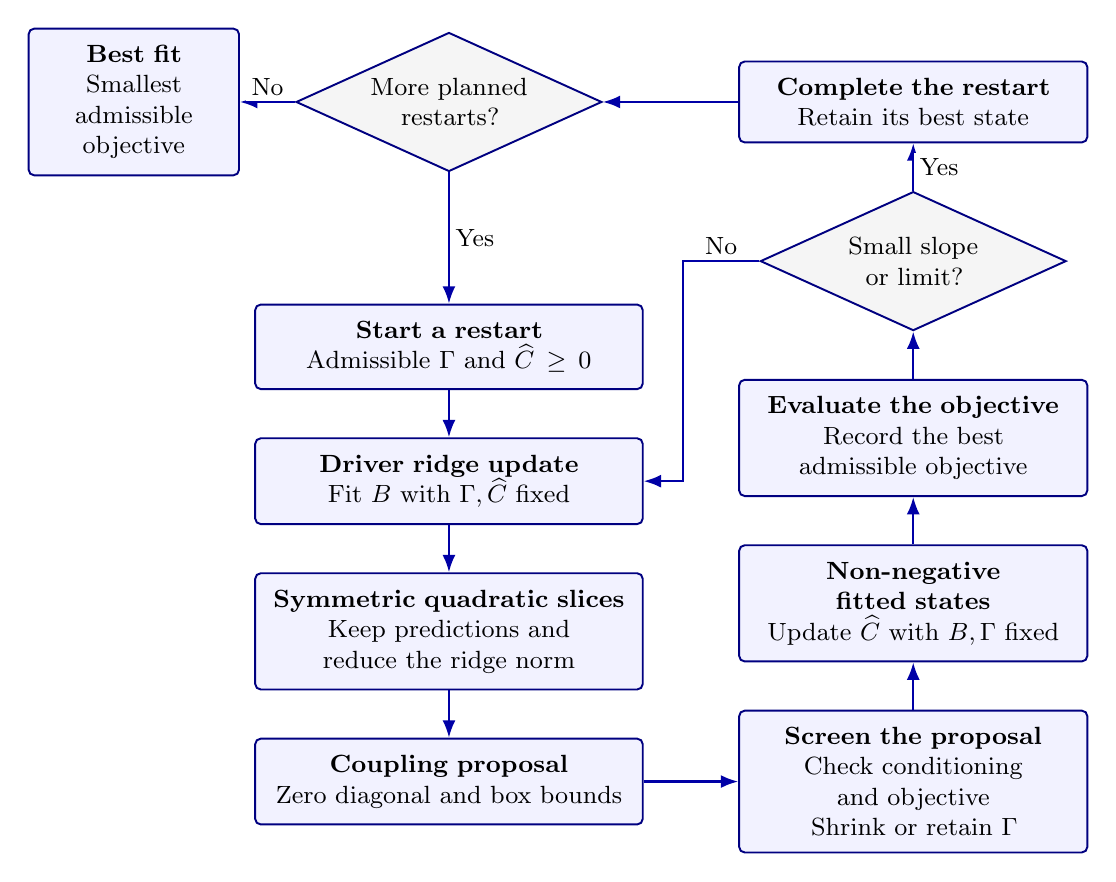
\begin{tikzpicture}[
    c5box/.style={draw=blue!50!black,fill=blue!5,rounded corners=2pt,
        line width=0.7pt,align=center,font=\small,inner sep=6pt},
    c5decision/.style={diamond,aspect=2.2,draw=blue!50!black,fill=black!4,
        line width=0.7pt,align=center,font=\small,text width=2.1cm,inner sep=2pt},
    c5arrow/.style={-{Latex[length=2.2mm]},draw=blue!65!black,line width=0.8pt},
    c5label/.style={font=\small,fill=white,inner sep=2pt}
]
\node[c5box,text width=4.5cm] (initialize) at (0,0)
    {\textbf{Start a restart}\\Admissible \(\Gamma\) and \(\widehat C\geq0\)};
\node[c5box,text width=4.5cm,below=6mm of initialize] (driver)
    {\textbf{Driver ridge update}\\Fit \(B\) with \(\Gamma,\widehat C\) fixed};
\node[c5box,text width=4.5cm,below=6mm of driver] (symmetry)
    {\textbf{Symmetric quadratic slices}\\Keep predictions and reduce the ridge norm};
\node[c5box,text width=4.5cm,below=6mm of symmetry] (proposal)
    {\textbf{Coupling proposal}\\Zero diagonal and box bounds};
\node[c5box,text width=4.0cm,right=12mm of proposal] (screen)
    {\textbf{Screen the proposal}\\Check conditioning\\and objective\\Shrink or retain \(\Gamma\)};
\node[c5box,text width=4.0cm,above=6mm of screen] (states)
    {\textbf{Non-negative fitted states}\\Update \(\widehat C\) with \(B,\Gamma\) fixed};
\node[c5box,text width=4.0cm,above=6mm of states] (record)
    {\textbf{Evaluate the objective}\\Record the best\\admissible objective};
\node[c5decision,above=6mm of record] (stop)
    {Small slope\\or limit?};
\node[c5box,text width=4.0cm,above=6mm of stop] (retain)
    {\textbf{Complete the restart}\\Retain its best state};
\node[c5decision] (restart) at (initialize.center |- retain.center)
    {More planned\\restarts?};
\node[c5box,text width=2.25cm,left=7mm of restart] (finish)
    {\textbf{Best fit}\\Smallest admissible objective};
\coordinate (loopcorner) at ($(initialize.east)+(5mm,0)$);
\draw[c5arrow] (initialize.south)--(driver.north);
\draw[c5arrow] (driver.south)--(symmetry.north);
\draw[c5arrow] (symmetry.south)--(proposal.north);
\draw[c5arrow] (proposal.east)--(screen.west);
\draw[c5arrow] (screen.north)--(states.south);
\draw[c5arrow] (states.north)--(record.south);
\draw[c5arrow] (record.north)--(stop.south);
\draw[c5arrow] (stop.north)--node[c5label,right] {Yes}(retain.south);
\draw[c5arrow] (stop.west)--node[c5label,above] {No}(loopcorner |- stop.west)
    --(loopcorner |- driver.east)--(driver.east);
\draw[c5arrow] (retain.west)--(restart.east);
\draw[c5arrow] (restart.south)--node[c5label,right] {Yes}(initialize.north);
\draw[c5arrow] (restart.west)--node[c5label,above] {No}(finish.east);
\end{tikzpicture}
\endgroup

\caption{Conceptual fitting cycle with explicit symmetry, conditioning, descent, and non-negativity checks. The prescribed restart count can be one.}
\label{fig:ch5_training_cycle}
\end{figure}

The cycle returns to the driver because each block changes the conditions faced by the remaining blocks. The conditioning screen is applied to the coupling proposal before the fitted-state update, and the complete objective is recorded after each full cycle. The restart decision belongs to the prescribed search procedure, while the final model selection compares the admissible objective values obtained. Together, these steps define the accepted sequence of updates for the nonconvex fit.

\begin{table}[htbp]
\centering
\caption{Specified fitting settings for the structured regression.}
\label{tab:icsor_fitting_settings}
\begin{tabular}{ll}
\toprule
Setting & Value\\
\midrule
Baseline feature & Included\\
Invariant penalty \(\lambda_{inv}\) & \(8.68\times10^{-3}\)\\
Coupled-system penalty \(\lambda_{sys}\) & \(1.27\times10^{-3}\)\\
Driver ridge penalty \(\lambda_B\) & \(6.09\times10^{-5}\)\\
Coupling ridge penalty \(\lambda_{\Gamma}\) & \(6.55\times10^{-4}\)\\
Off-diagonal bound \(\gamma_{abs}\) & 0.368\\
Maximum full fitting cycles & 60\\
Restarts & 1\\
Trailing objective window & 12 cycles\\
Objective slope tolerance & \(2.85\times10^{-7}\)\\
\bottomrule
\end{tabular}
\end{table}

Table~\ref{tab:icsor_fitting_settings} summarizes the numerical choices used during fitting. The condition threshold \(\kappa_{max}\) is an additional prescribed safeguard and is checked independently of the coefficient bound. Hyperparameter assessment uses validation observations drawn only from the training pool. Held-out test responses do not determine the penalty weights or stopping settings \citep{Kaufman2012}. The fitted settings are held fixed within each sample-size comparison so that changes in the learning curves reflect differences in available data rather than changes in the model specification.

\subsection{Checked deployment}

\subsubsection{The raw coupled state}

For a new input pair \((u_*,c_{in,*})\), the fitted parameters define
\begin{equation}
\equationname{Raw deployed state from the fitted coupled system}
\label{eq:icsor_raw_state}
\widehat R=I_F-\widehat\Gamma,
\qquad d_* =\widehat B\phi(u_*,c_{in,*}),
\qquad \widehat R c_{raw}=d_*.
\end{equation}
The notation \(c_{raw}=\widehat R^{-1}d_*\) describes the mapping mathematically, although the prediction is evaluated numerically by solving the linear system. The adopted conditioning bound limits the sensitivity of that solve. The raw state can be returned directly only if it satisfies both the invariant and non-negativity checks.

The two diagnostics measure different departures from physical admissibility. For a vector, the Euclidean norm is the square root of the sum of squared entries, so an invariant-residual vector \((3,4)^\top\) has norm 5. For an illustrative concentration vector \((-0.3,0.1,-0.4)^\top\), retaining only the negative entries gives \((-0.3,0,-0.4)^\top\), whose absolute norm is 0.7. The first quantity measures the size of a mass conservation discrepancy; the second measures the total negative concentration in the adopted numerical coordinates.

For a candidate state \(c\), define
\begin{equation}
\equationname{Mass conservation and non-negativity diagnostics of a deployed state}
\label{eq:icsor_deployment_diagnostics}
v_{mc}(c)=\|A(c-c_{in,*})\|_2,
\qquad
v_{nn}(c)=\|\min(c,\mathbf{0})\|_1.
\end{equation}
The minimum is evaluated componentwise. The numerical diagnostic tolerance is \(10^{-10}\). The mathematical requirements are exact equality and non-negativity; the residual tolerance defines their computational assessment under the stated scaling of \(A\).

\subsubsection{Affine projection for mass conservation}

The first correction stage enforces the mass conservation equalities without yet imposing concentration bounds. The underlying geometry can again be seen in the two-component example. Let the raw prediction be \((p_1,p_2)^\top\) and let the required total inventory be \(T\). The nearest mass-conserving state minimizes \((c_1-p_1)^2+(c_2-p_2)^2\) subject to \(c_1+c_2=T\). Introducing multiplier \(\eta\) gives
\begin{equation}
\equationname{Lagrangian for an illustrative two-component affine projection}
\label{eq:icsor_scalar_projection_lagrangian}
\mathcal{L}=\frac{1}{2}(c_1-p_1)^2+
\frac{1}{2}(c_2-p_2)^2+\eta(c_1+c_2-T).
\end{equation}
The stationarity and equality conditions are
\begin{equation}
\equationname{Stationarity and equality conditions for the illustrative affine projection}
\label{eq:icsor_scalar_projection_conditions}
c_1-p_1+\eta=0,
\qquad c_2-p_2+\eta=0,
\qquad c_1+c_2=T.
\end{equation}
Thus
\begin{equation}
\equationname{Closed-form solution of the illustrative affine projection}
\label{eq:icsor_scalar_projection_solution}
\begin{aligned}
\eta&=\frac{p_1+p_2-T}{2},\\
c_1&=p_1-\frac{p_1+p_2-T}{2},\\
c_2&=p_2-\frac{p_1+p_2-T}{2}.
\end{aligned}
\end{equation}
The unweighted projection distributes the inventory discrepancy equally between the two numerical coordinates. For \(p_1=12\), \(p_2=1\), and \(T=10\), the discrepancy is 3, so the multiplier is 1.5 and the projected state is \((10.5,-0.5)^\top\). The total inventory is correct, but the second concentration is negative. This example shows why an equality-only projection cannot guarantee complete physical admissibility.

In the full component space, a raw state that fails the checks is first projected by
\begin{equation}
\equationname{Euclidean affine projection onto the mass conservation equality}
\label{eq:icsor_affine_problem}
c_{aff}=\mathop{\arg\min}_{c\in\mathbb{R}^{F}}\|c-c_{raw}\|_2^2
\quad\text{subject to}\quad Ac=Ac_{in,*}.
\end{equation}
With multiplier \(\eta\in\mathbb{R}^{K}\), stationarity gives \(c-c_{raw}+A^\top\eta=0\). Substitution into the equality yields \(AA^\top\eta=A(c_{raw}-c_{in,*})\), and full row rank of \(A\) gives
\begin{equation}
\equationname{Closed-form affine projection of the raw component state}
\label{eq:icsor_affine_solution}
c_{aff}=c_{raw}-A^\top(AA^\top)^{-1}A(c_{raw}-c_{in,*}).
\end{equation}
Because \(A\) is fixed, the matrix \(A^\top(AA^\top)^{-1}A\) can be prepared once and reused for every new prediction.

The two-component example makes the same matrix operation explicit:
\begin{equation}
\equationname{Illustrative matrix of the mass conservation projection}
\label{eq:icsor_small_affine_matrix}
AA^\top=2,
\qquad
A^\top(AA^\top)^{-1}A
=\frac{1}{2}\begin{bmatrix}1&1\\1&1\end{bmatrix}.
\end{equation}
With illustrative influent \((6,4)^\top\), the raw-minus-influent difference is \((6,-3)^\top\). Multiplication by the projection matrix gives \((1.5,1.5)^\top\), which is subtracted from the raw state. The matrix calculation therefore reproduces the scalar result without requiring an arbitrary choice about which component should absorb the imbalance.

Geometrically, this is the orthogonal projection onto the affine set defined by the adopted mass conservation equations in the chosen numerical component coordinates. It removes the part of the raw prediction normal to that set while retaining the tangent component. Because the distance is measured in the stated component units, the scaling of those coordinates affects the adjustment. \citet{SturmSilva2024} develop related mass-conservation projections and show why species-dependent weighting matters when concentration scales differ.

The affine state is checked for both balance residuals and non-negativity before it is accepted. The equality follows analytically from Equation~\eqref{eq:icsor_affine_solution}, but the numerical residual check can still reveal inconsistency in the operator or computation. If the affine state remains negative, a second projection must enforce the equality and inequality requirements simultaneously.

\subsubsection{Joint mass conservation and non-negativity}

The final projection can again be understood from the two-component example. Starting from the mass-conserving but negative state \((10.5,-0.5)^\top\), require \(c_1+c_2=10\) and \(c_1,c_2\geq0\). Introduce non-negative adjustment variables \(\rho_1,\rho_2\) satisfying
\begin{equation}
\equationname{Absolute-adjustment bounds for an illustrative two-component projection}
\label{eq:icsor_scalar_absolute_constraints}
\begin{aligned}
\rho_1&\geq c_1-10.5,&\rho_1&\geq10.5-c_1,\\
\rho_2&\geq c_2+0.5,&\rho_2&\geq-0.5-c_2.
\end{aligned}
\end{equation}
These inequalities make \(\rho_1\) and \(\rho_2\) at least as large as the absolute adjustments of the two coordinates. Minimizing \(w_1\rho_1+w_2\rho_2\) with positive weights makes them equal to those absolute adjustments at the optimum.

Imposing the inventory equality with \(c_2=t\) gives \(c_1=10-t\) and \(0\leq t\leq10\). Both absolute adjustments are then \(t+0.5\), so the objective becomes \((w_1+w_2)(t+0.5)\). It is minimized at \(t=0\), yielding \((10,0)^\top\). With equal weights, this state has cost 1, whereas \(t=1\) would give \((9,1)^\top\) with cost 3. The reduced example therefore makes the optimal joint correction transparent.

For the full component state, the final projection is
\begin{equation}
\equationname{Weighted absolute-distance projection for mass conservation and non-negativity}
\label{eq:icsor_weighted_correction}
\begin{aligned}
\widehat c =\mathop{\arg\min}_{c,\rho\in\mathbb{R}^{F}}\quad
& w_c^\top\rho\\
\text{subject to}\quad
& Ac=Ac_{in,*},\\
& c\geq\mathbf{0},\\
& -\rho\leq c-c_{aff}\leq\rho,\\
& \rho\geq\mathbf{0}.
\end{aligned}
\end{equation}
For strictly positive weights \(w_c\), the optimal auxiliary variable satisfies \(\rho_f=|c_f-c_{aff,f}|\). The objective is therefore the weighted absolute adjustment \(\sum_f w_{c,f}|c_f-c_{aff,f}|\). The fitted regression itself remains unchanged; only the returned state is corrected.

The problem is linear because the absolute values are represented by auxiliary variables and linear inequalities. The revised-simplex method described by \citet{HuangfuHall2018} provides an algorithmic basis for this type of projection. The mathematical feasible set is nonempty whenever the supplied influent state is non-negative and satisfies the adopted boundary relation. Positive weights make the objective bounded below and discourage unnecessary movement in every component. A minimizer therefore exists, although several minimizing states can occur if the weighted absolute-distance objective contains a flat face.

The weights determine how the required adjustment is distributed. A large weight makes a component expensive to change, whereas a smaller weight allows more movement if that helps satisfy the constraints. The weights are fixed before deployment according to the intended component scaling and scientific priorities. Equal numerical weights are themselves a modeling choice because the components differ in units and typical magnitudes.

A three-component illustration shows how this choice matters. Let the invariant row be \([1\ \ 1\ \ 1]\), and let the affine reference be \((-1,4,7)^\top\), whose total is 10. Restoring the first component to zero requires one unit to be removed elsewhere. Two feasible candidates are \((0,3,7)^\top\) and \((0,4,6)^\top\). With weights \((1,10,1)^\top\), their costs are 11 and 2, respectively, so the second candidate is preferred because changing the second component is expensive. With weights \((1,1,10)^\top\), the costs reverse to 2 and 11. Both candidates conserve the same total inventory; the weights determine which admissible redistribution is preferred.

\citet{KircherVotsmeier2025} show why mass-conservation projection in reaction-kinetics surrogates must be combined with non-negativity enforcement. Their scaled-space formulation protects low-concentration species during correction. Equation~\eqref{eq:icsor_weighted_correction} addresses the same joint requirement for activated sludge components through a weighted absolute-distance formulation. It enforces the adopted linear invariants and non-negativity on the final returned state.

\subsubsection{Illustrative projection and the failure of clipping}

The difference between projection and simple clipping can be summarized using the same two-component system. Let \(A=[1\ \ 1]\), let the influent inventory total be 10, and let the raw prediction be \(c_{raw}=(12,1)^\top\). The raw total is 13. The affine projection subtracts 1.5 from each coordinate, producing \(c_{aff}=(10.5,-0.5)^\top\). Mass conservation is restored, but the second component becomes negative.

If that negative concentration is clipped to zero, the state becomes \((10.5,0)^\top\), whose total is 10.5 and therefore violates the invariant. Equation~\eqref{eq:icsor_weighted_correction}, by contrast, returns \((10,0)^\top\) for equal weights. Both requirements are satisfied simultaneously. The distinction is important because repairing one physical defect independently can recreate another.

The deployment procedure therefore follows the geometry of the feasible set. A raw state that already satisfies both checks is returned without modification. Otherwise, the affine projection first restores the invariant relations. If that state is also non-negative, it can be returned. The linear program is needed only when the affine state remains outside the non-negative region. Every returned candidate is then checked under the declared numerical tolerances, and a failed solve or failed final audit is recorded as a prediction failure.

Figure~\ref{fig:ch5_checked_deployment} makes these branches explicit.

\begin{figure}[htbp]
\centering
\begingroup\linespread{1}\selectfont
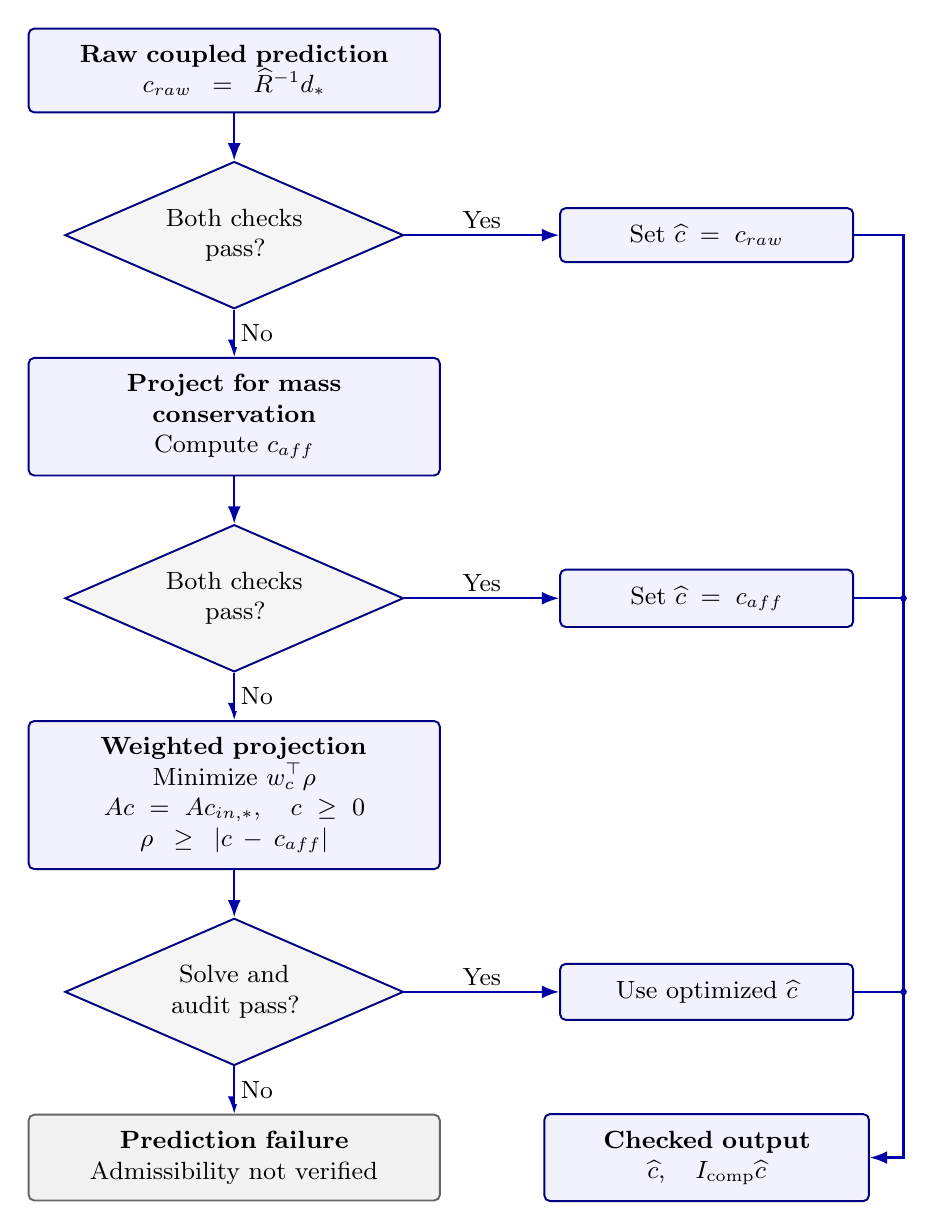
\begin{tikzpicture}[
    c5box/.style={draw=blue!50!black,fill=blue!5,rounded corners=2pt,
        line width=0.7pt,align=center,font=\small,inner sep=6pt},
    c5decision/.style={diamond,aspect=2.3,draw=blue!50!black,fill=black!4,
        line width=0.7pt,align=center,font=\small,text width=2.3cm,inner sep=2pt},
    c5arrow/.style={-{Latex[length=2.2mm]},draw=blue!65!black,line width=0.8pt},
    c5label/.style={font=\small,fill=white,inner sep=2pt}
]
\node[c5box,text width=4.8cm] (raw) at (0,0)
    {\textbf{Raw coupled prediction}\\\(c_{raw}=\widehat R^{-1}d_*\)};
\node[c5decision,below=6mm of raw] (rawcheck)
    {Both checks\\pass?};
\node[c5box,text width=3.3cm] (rawaccept) at (6,0 |- rawcheck.center)
    {Set \(\widehat c=c_{raw}\)};
\node[c5box,text width=4.8cm,below=6mm of rawcheck] (affine)
    {\textbf{Project for mass conservation}\\Compute \(c_{aff}\)};
\node[c5decision,below=6mm of affine] (affcheck)
    {Both checks\\pass?};
\node[c5box,text width=3.3cm] (affaccept) at (6,0 |- affcheck.center)
    {Set \(\widehat c=c_{aff}\)};
\node[c5box,text width=4.8cm,below=6mm of affcheck] (projection)
    {\textbf{Weighted projection}\\Minimize \(w_c^\top\rho\)\\\(Ac=Ac_{in,*},\quad c\geq0\)\\\(\rho\geq|c-c_{aff}|\)};
\node[c5decision,below=6mm of projection] (audit)
    {Solve and\\audit pass?};
\node[c5box,text width=3.3cm] (lpaccept) at (6,0 |- audit.center)
    {Use optimized \(\widehat c\)};
\node[c5box,text width=4.8cm,fill=black!5,draw=black!60,below=6mm of audit] (failed)
    {\textbf{Prediction failure}\\Admissibility not verified};
\node[c5box,text width=3.7cm] (return) at (6,0 |- failed.center)
    {\textbf{Checked output}\\\(\widehat c,\quad I_{\mathrm{comp}}\widehat c\)};
\coordinate (merge) at (8.5,0);
\draw[c5arrow] (raw.south)--(rawcheck.north);
\draw[c5arrow] (rawcheck.east)--node[c5label,above] {Yes}(rawaccept.west);
\draw[c5arrow] (rawcheck.south)--node[c5label,right] {No}(affine.north);
\draw[c5arrow] (affine.south)--(affcheck.north);
\draw[c5arrow] (affcheck.east)--node[c5label,above] {Yes}(affaccept.west);
\draw[c5arrow] (affcheck.south)--node[c5label,right] {No}(projection.north);
\draw[c5arrow] (projection.south)--(audit.north);
\draw[c5arrow] (audit.east)--node[c5label,above] {Yes}(lpaccept.west);
\draw[c5arrow] (audit.south)--node[c5label,right] {No}(failed.north);
\draw[c5arrow] (rawaccept.east)--(merge |- rawaccept.east)
    --(merge |- return.east)--(return.east);
\draw[draw=blue!65!black,line width=0.8pt] (affaccept.east)--(merge |- affaccept.east);
\draw[draw=blue!65!black,line width=0.8pt] (lpaccept.east)--(merge |- lpaccept.east);
\fill[blue!65!black] (merge |- affaccept.east) circle (1.2pt);
\fill[blue!65!black] (merge |- lpaccept.east) circle (1.2pt);
\end{tikzpicture}
\endgroup

\caption{Checked deployment of one predicted component state. Accepted branches merge before the common reporting map is applied. A failed final audit produces a reported prediction failure.}
\label{fig:ch5_checked_deployment}
\end{figure}

The illustrative state \((12,1)^\top\) follows both ``No'' branches because the raw inventory is incorrect and the affine projection contains a negative concentration. The weighted projection produces \((10,0)^\top\), which enters the return branch only after both checks pass. A state that satisfies the requirements earlier in the sequence reaches the same reporting step with less projection effort. The branches therefore differ in computational work, but not in the physical acceptance requirements.

The final component state is the deployed model output. The corresponding reported water-quality quantities are
\begin{equation}
\equationname{Water-quality composites of the final checked state}
\label{eq:icsor_deployed_composites}
\widehat y_{\mathrm{comp}}=I_{\mathrm{comp}}\widehat c.
\end{equation}
The deployment constraints determine whether the state is admissible, while the stage-wise assessment records how often each correction stage is needed.

\subsection{Interpreting the complete prediction map}

\subsubsection{Driver coefficients and back projection}

The effect of component coupling on coefficient interpretation can be seen using the same two-component example. Take the coupling matrix from Equation~\eqref{eq:icsor_small_coupling_matrices}, a reduced feature vector \((1,a)^\top\), and driver coefficients
\begin{equation}
\equationname{Illustrative driver coefficients and operating-dependent driver}
\label{eq:icsor_small_driver_coefficient_matrix}
B=\begin{bmatrix}4&1\\2&0\end{bmatrix},
\qquad
r=\begin{bmatrix}4+a\\2\end{bmatrix}.
\end{equation}
The first coefficient column gives the baseline response, and the second gives direct dependence on the hypothetical scalar input \(a\). Passing these coefficients through the coupling inverse gives
\begin{equation}
\equationname{Illustrative transformation of driver coefficients through coupling}
\label{eq:icsor_small_back_projection}
\begin{aligned}
R^{-1}B
&=\frac{1}{0.96}
\begin{bmatrix}1&0.2\\0.2&1\end{bmatrix}
\begin{bmatrix}4&1\\2&0\end{bmatrix}\\
&=\frac{1}{0.96}\begin{bmatrix}4.4&1\\2.8&0.2\end{bmatrix}
=\begin{bmatrix}55/12&25/24\\35/12&5/24\end{bmatrix}.
\end{aligned}
\end{equation}
The second raw component now depends on \(a\), even though its own driver coefficient for that input was zero. The dependence is introduced by the simultaneous coupling solve. A coefficient in the driver is therefore not, by itself, the coefficient of the final raw component response.

The same transformation continues into reported water-quality quantities. For a hypothetical quantity \(y=c_1+2c_2\), with reporting row \([1\ \ 2]\),
\begin{equation}
\equationname{Illustrative composite coefficients after coupling}
\label{eq:icsor_small_composite_projection}
\begin{bmatrix}1&2\end{bmatrix}R^{-1}B
=\begin{bmatrix}125/12&35/24\end{bmatrix}.
\end{equation}
At \(a=2\), the driver is \((6,2)^\top\), the raw component state is \((20/3,10/3)^\top\), and the reported quantity is \(40/3\). The transformed coefficient row gives the same value through \(125/12+(35/24)2=40/3\). The example shows how the driver coefficients acquire their final raw-response meaning only after coupling and reporting have been applied.

For the fitted model, the raw component coefficient matrix is
\begin{equation}
\equationname{Raw component-response coefficients after coupling}
\label{eq:icsor_raw_component_coefficients}
B_{\mathrm{raw}}=\widehat R^{-1}\widehat B,
\qquad c_{raw}=B_{\mathrm{raw}}\phi.
\end{equation}
The corresponding coefficient map for COD, TN, TP, and TSS is
\begin{equation}
\equationname{Raw composite-response coefficients after coupling and reporting}
\label{eq:icsor_raw_composite_coefficients}
B_{\mathrm{raw,comp}}=I_{\mathrm{comp}}\widehat R^{-1}\widehat B,
\qquad y_{\mathrm{raw,comp}}=B_{\mathrm{raw,comp}}\phi.
\end{equation}
This transformation carries the driver coefficients first through the learned component coupling and then through the reporting map. Consequently, inspection of a COD quadratic term uses the COD row of \(B_{\mathrm{raw,comp}}\), rather than an arbitrary component row of \(\widehat B\).

Figure~\ref{fig:ch5_prediction_chain} summarizes this raw prediction chain while retaining the named feature blocks.

\begin{figure}[htbp]
\centering
\begingroup\linespread{1}\selectfont
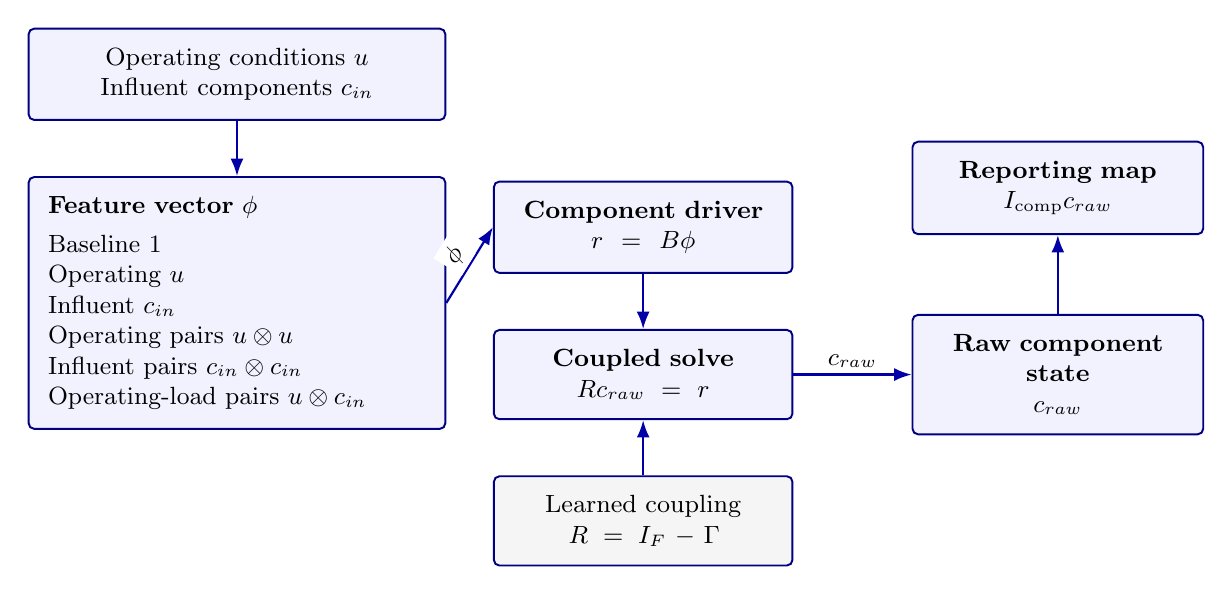
\begin{tikzpicture}[
    c5box/.style={draw=blue!50!black,fill=blue!5,rounded corners=2pt,
        line width=0.7pt,align=center,font=\small,inner sep=7pt},
    c5feature/.style={c5box,text width=4.8cm,align=left},
    c5arrow/.style={-{Latex[length=2.2mm]},draw=blue!65!black,line width=0.8pt},
    c5label/.style={font=\small,fill=white,inner sep=2pt}
]
\node[c5box,text width=4.8cm] (inputs) at (0,0)
    {Operating conditions \(u\)\\Influent components \(c_{in}\)};
\node[c5feature,below=7mm of inputs] (features)
    {\textbf{Feature vector \(\phi\)}\\[3pt]
     Baseline \(1\)\\
     Operating \(u\)\\
     Influent \(c_{in}\)\\
     Operating pairs \(u\otimes u\)\\
     Influent pairs \(c_{in}\otimes c_{in}\)\\
     Operating-load pairs \(u\otimes c_{in}\)};
\node[c5box,text width=3.3cm] (driver) at ($(features.north east)+(2.5cm,-0.65cm)$)
    {\textbf{Component driver}\\\(r=B\phi\)};
\node[c5box,text width=3.3cm,below=7mm of driver] (solve)
    {\textbf{Coupled solve}\\\(Rc_{raw}=r\)};
\node[c5box,text width=3.3cm,fill=black!4,below=7mm of solve] (coupling)
    {Learned coupling\\\(R=I_F-\Gamma\)};
\node[c5box,text width=3.2cm,right=15mm of solve] (components)
    {\textbf{Raw component}\\\textbf{state}\\\(c_{raw}\)};
\node[c5box,text width=3.2cm,above=10mm of components] (reported)
    {\textbf{Reporting map}\\\(I_{\mathrm{comp}}c_{raw}\)};
\draw[c5arrow] (inputs.south)--(features.north);
\draw[c5arrow] (features.east)--node[c5label,above,sloped] {\(\phi\)}(driver.west);
\draw[c5arrow] (driver.south)--(solve.north);
\draw[c5arrow] (coupling.north)--(solve.south);
\draw[c5arrow] (solve.east)--node[c5label,above] {\(c_{raw}\)}(components.west);
\draw[c5arrow] (components.north)--(reported.south);
\end{tikzpicture}
\endgroup

\caption{Named feature blocks and the transformation from driver to raw component and reported-composite predictions. Composing the three operations gives the raw reported coefficient map \(I_{\mathrm{comp}}R^{-1}B\).}
\label{fig:ch5_prediction_chain}
\end{figure}

In the two-feature illustration, the second driver has no direct coefficient for the scalar input, but the coupling step gives the corresponding component a nonzero response. The reporting map then combines both component responses. Reading the calculation in this order explains the back projection in Equations~\eqref{eq:icsor_small_back_projection} and \eqref{eq:icsor_small_composite_projection}. Checked deployment occurs afterward and may further modify the component state before the final reported quantities are calculated.

The fitted coefficients are displayed according to the same logical structure. Operating terms are separated from influent terms, symmetric quadratic maps display the mirrored cells consistently, and operating-load maps show which operating variables interact with which influent components. The coupling matrix is displayed separately because its meaning differs from that of the driver coefficients.

A post-fitting display threshold is used only to simplify presentation. For each reported-composite raw-regression map, the threshold is \(10^{-4}\) times the largest absolute coefficient. For the coupling matrix, it is \(10^{-4}\) times the largest absolute off-diagonal entry. The fitted model itself remains unchanged; the threshold controls only which entries are shown. Symmetric quadratic summaries count unique upper-triangular terms. A small coefficient can still contribute substantially when multiplied by a large feature, so interpretation considers coefficient magnitude together with the scale of the corresponding input and its contribution over the declared domain \citep{Selerio2026,Nazlabadi2021}.

\subsubsection{Analytical jacobians of the raw regression}

A fitted coefficient and a local response derivative are not the same quantity. The scalar driver in Equation~\eqref{eq:icsor_scalar_driver_example} makes this distinction explicit:
\begin{equation}
\equationname{Gradients of the illustrative scalar regression driver}
\label{eq:icsor_scalar_driver_derivatives}
\begin{aligned}
\frac{\partial r_1}{\partial u_1}&=2+0.2u_1+0.2u_2,\\
\frac{\partial r_1}{\partial u_2}&=-1+0.2u_1+0.25c_1,\\
\frac{\partial r_1}{\partial c_1}&=0.5+0.25u_2,
&\frac{\partial r_1}{\partial c_2}&=-0.1c_2.
\end{aligned}
\end{equation}
At \(u=(2,3)^\top\) and \(c=(4,5)^\top\), these derivatives are 3, 0.4, 1.25, and \(-0.5\). The derivative with respect to \(u_1\) is therefore 3 even though the linear coefficient of \(u_1\) is only 2. The difference comes from the operating curvature and interaction terms.

The second illustrative driver \(r_2=-u_1+u_2+0.2c_2\) has derivative \(-1\) with respect to \(u_1\). Differentiating the coupled equations while holding the learned coupling fixed gives
\[
\frac{\partial c_1}{\partial u_1}-0.2\frac{\partial c_2}{\partial u_1}=3,
\qquad
-0.2\frac{\partial c_1}{\partial u_1}+\frac{\partial c_2}{\partial u_1}=-1.
\]
The same inverse used for prediction therefore propagates the derivative:
\begin{equation}
\equationname{Illustrative propagation of an operating derivative through coupling}
\label{eq:icsor_small_chain_derivative}
\begin{bmatrix}\partial c_1/\partial u_1\\\partial c_2/\partial u_1\end{bmatrix}
=\frac{1}{0.96}\begin{bmatrix}1&0.2\\0.2&1\end{bmatrix}
\begin{bmatrix}3\\-1\end{bmatrix}
=\begin{bmatrix}35/12\\-5/12\end{bmatrix}.
\end{equation}
For the hypothetical reporting row \([1\ \ 2]\), the resulting reported derivative is \(35/12+2(-5/12)=25/12\). Differentiating the driver, passing the derivative through coupling, and applying the reporting weights are therefore distinct stages of the same sensitivity calculation.

Collecting several derivatives produces a Jacobian. At the illustrative operating point,
\begin{equation}
\equationname{Illustrative operating Jacobians before and after coupling}
\label{eq:icsor_small_operating_jacobian}
J_{r,u}=\begin{bmatrix}3&0.4\\-1&1\end{bmatrix},
\qquad
R^{-1}J_{r,u}=\begin{bmatrix}35/12&5/8\\-5/12&9/8\end{bmatrix}.
\end{equation}
The first column reproduces the derivative calculation above. The second is obtained by solving the same coupled system for derivative column \((0.4,1)^\top\). The Jacobian therefore collects the local response of the complete raw mapping to several inputs at once.

For component \(f\), reshape the operating-load coefficients as \(H_{uc}^{(f)}\in\mathbb{R}^{M_{op}\times F}\), so that the interaction term is \(u^\top H_{uc}^{(f)}c_{in}\). The component driver can then be written as
\begin{equation}
\equationname{Component driver expressed through symmetric quadratic matrices}
\label{eq:icsor_driver_component}
\begin{aligned}
r_f={}&b_f+(W_u)_{f,:}u+(W_{in})_{f,:}c_{in}
+u^\top Q_{uu}^{(f)}u\\
&+c_{in}^\top Q_{cc}^{(f)}c_{in}
+u^\top H_{uc}^{(f)}c_{in}.
\end{aligned}
\end{equation}
With symmetric quadratic slices, its gradients are
\begin{equation}
\equationname{Operating and influent gradients of a component driver}
\label{eq:icsor_driver_gradients}
\begin{aligned}
\nabla_u r_f&=(W_u)_{f,:}^\top+2Q_{uu}^{(f)}u
+H_{uc}^{(f)}c_{in},\\
\nabla_{c_{in}}r_f&=(W_{in})_{f,:}^\top+2Q_{cc}^{(f)}c_{in}
+(H_{uc}^{(f)})^\top u.
\end{aligned}
\end{equation}
These expressions follow directly from differentiation. For \(x^\top Qx\), the derivative collects both mirrored terms and reduces to \(2Qx\) when \(Q\) is symmetric. For \(u^\top Hc\), differentiation gives \(Hc\) with respect to \(u\) and \(H^\top u\) with respect to \(c\).

Stacking the component gradients gives the driver Jacobians \(J_{r,u}\in\mathbb{R}^{F\times M_{op}}\) and \(J_{r,c}\in\mathbb{R}^{F\times F}\). The corresponding raw component and composite Jacobians are
\begin{equation}
\equationname{Raw component and composite Jacobians after coupling}
\label{eq:icsor_raw_jacobians}
\begin{aligned}
J_{raw,u}&=\widehat R^{-1}J_{r,u},
&J_{raw,c}&=\widehat R^{-1}J_{r,c},\\
J_{raw,comp,u}&=I_{\mathrm{comp}}J_{raw,u},
&J_{raw,comp,c}&=I_{\mathrm{comp}}J_{raw,c}.
\end{aligned}
\end{equation}
These derivatives describe the complete fitted raw regression at a specified operating point, including the effects of curvature, interactions, coupling, and reporting. Projection-stage derivatives are considered separately below.

For example, an aeration sensitivity can be evaluated at low and high ammonium loading while other inputs are held fixed. A difference between the two derivatives indicates a loading-dependent association in the fitted response. Oxygen-transfer limitations and heterotrophic competition provide process context for interpreting such a pattern \citep{StenstromSong1991}. The process model therefore provides a plausibility reference for the learned relationship without converting that statistical relationship into a causal claim.

\subsubsection{Sensitivity after the affine projection}

Projection can substantially alter the local response of the fitted model. Return to the two-feature example in Equation~\eqref{eq:icsor_small_back_projection}. Its raw derivative with respect to \(a\) is \((25/24,5/24)^\top\), whose entries sum to \(5/4\). This raw response changes the total inventory. If the influent inventory is fixed, the affine projection must remove that total change.

For the two-component invariant,
\begin{equation}
\equationname{Illustrative operating derivative after affine projection}
\label{eq:icsor_small_projection_derivative}
\begin{aligned}
P_A&=\frac{1}{2}\begin{bmatrix}1&-1\\-1&1\end{bmatrix},\\
\frac{\partial c_{aff}}{\partial a}
&=P_A\begin{bmatrix}25/24\\5/24\end{bmatrix}
=\begin{bmatrix}5/12\\-5/12\end{bmatrix}.
\end{aligned}
\end{equation}
The projected derivatives now sum to zero, as required by the fixed total inventory. For reporting row \([1\ \ 2]\), the projected derivative is \(5/12+2(-5/12)=-5/12\), whereas the raw derivative was \(35/24\). Projection therefore changes both the magnitude and sign of the local reported response because it enforces a different material-accounting condition on the complete state.

Influent sensitivities involve an additional effect because perturbing the influent also changes the mass conservation reference. In the reduced example, suppose the driver has no influent term. Increasing either influent component by \(\delta\) increases the required total by \(\delta\). The unweighted affine projection then adds \(\delta/2\) to each predicted component. The resulting influent derivative is \(\frac12\begin{bmatrix}1&1\\1&1\end{bmatrix}\), even though the raw regression has zero direct influent sensitivity. This contribution arises entirely from the changing right-hand side of the physical equality.

Define
\begin{equation}
\equationname{Complementary mass conservation projection matrices}
\label{eq:icsor_projection_matrices}
Q_A=A^\top(AA^\top)^{-1}A,
\qquad P_A=I_F-Q_A.
\end{equation}
Then \(c_{aff}=P_Ac_{raw}+Q_Ac_{in}\), and with the fitted coefficients and invariant operator held fixed,
\begin{equation}
\equationname{Operating and influent Jacobians of the affine-projected state}
\label{eq:icsor_affine_jacobians}
J_{aff,u}=P_AJ_{raw,u},
\qquad J_{aff,c}=P_AJ_{raw,c}+Q_A.
\end{equation}
The \(Q_A\) term in the influent derivative accounts for the changing conservation reference.

These expressions satisfy \(AJ_{aff,u}=0\) and \(AJ_{aff,c}=A\). An operating perturbation therefore changes the affine prediction only in directions that preserve the current influent inventories, while an influent perturbation changes those inventories consistently with the perturbed influent state. These identities also provide analytical checks on the sensitivity implementation.

When the same affine branch remains active over a local neighborhood, these Jacobians describe that branch. The complete deployment rule, however, can transition among raw, affine, and linear-program branches. Each branch therefore has its own local sensitivity \citep{Selerio2026}.

\subsubsection{Active constraints in the final projection}

A non-negativity boundary can change the derivative again. For the same reduced example, the affine components are
\begin{equation}
\equationname{Illustrative affine-projected components as functions of an operating input}
\label{eq:icsor_small_affine_branch}
c_{aff,1}=\frac{35}{6}+\frac{5a}{12},
\qquad
c_{aff,2}=\frac{25}{6}-\frac{5a}{12}.
\end{equation}
Their sum is 10. Near \(a=10\), the first component remains positive while the second reaches zero. Immediately below the boundary, the affine state is feasible and has derivative \((5/12,-5/12)^\top\). Above the boundary, the second affine component becomes negative, and the positive-weight absolute projection returns \((10,0)^\top\). The deployed derivative then becomes \((0,0)^\top\). The final response therefore has different local behavior on the two sides of the active constraint.

The same result follows by differentiating the active equalities. In the projected branch, the binding conditions are \(c_1+c_2=10\) and \(c_2=0\). Differentiation gives
\[
\frac{\partial c_1}{\partial a}+\frac{\partial c_2}{\partial a}=0,
\qquad
\frac{\partial c_2}{\partial a}=0,
\]
which implies a zero derivative for both components. The general active-set calculation extends this idea to all binding conservation and adjustment constraints.

The linear program can activate a zero-concentration bound or one of the absolute-adjustment inequalities. These binding constraints define the active set. If the optimal solution is unique and its nondegenerate basis remains unchanged over a local neighborhood, the solution varies affinely with the relevant right-hand sides. A local branch-specific sensitivity can then be obtained directly from that fixed basis.

At an active-set transition, however, the derivative can change abruptly. If several optimal projected states exist, the returned response can also depend on the rule used to select among them. Local deployment sensitivity is therefore assessed either by differentiating a verified fixed basis or by perturbing admissible inputs and resolving the complete deployment problem. Any branch change is recorded as part of that sensitivity assessment.

This distinction prevents three different interpretive quantities from being conflated. A driver coefficient belongs to \(\widehat B\). A raw-state sensitivity includes the effect of \(\widehat R^{-1}\). A deployed-state sensitivity additionally depends on the mass conservation reference and any active projection constraints. Each describes a different stage of the prediction.

\subsubsection{Following sensitivity through projection}

Interpretation must therefore follow the complete prediction map rather than stop at the fitted polynomial. Coupling transforms the driver into component predictions, the reporting map converts those components into water-quality quantities, and active projection constraints can alter the local derivative of the final state. Physical-unit interpretation should therefore specify whether it concerns a driver coefficient, a raw response derivative, or the derivative of the final projected prediction \citep{Brunton2016,Shen2023}.

A second hypothetical example isolates the effect of projection. Let a dimensionless operating input be \(a\), and define the raw concentrations
\[
c_{raw,1}(a)=4+a,\qquad c_{raw,2}(a)=3+2a.
\]
The raw slopes are one and two. At \(a=2\), the concentrations are 6 and 7, giving a total of 13. Suppose the required total is 10 and the projection minimizes the sum of squared adjustments with equal weights. If the adjustments are \(d_1\) and \(d_2\), conservation requires \(d_1+d_2=-3\). Substituting \(d_2=-3-d_1\) into the objective gives
\[
\begin{aligned}
d_1^2+d_2^2&=d_1^2+(-3-d_1)^2,\\
\frac{\mathrm d}{\mathrm d d_1}\bigl[d_1^2+(-3-d_1)^2\bigr]
&=4d_1+6=0.
\end{aligned}
\]
Thus \(d_1=d_2=-1.5\), giving the mass-conserving state \((4.5,5.5)^\top\).

For general \(a\), the excess total is \((4+a)+(3+2a)-10=3a-3\). Equal-weight affine projection subtracts half of that excess from each coordinate:
\[
\begin{aligned}
c_{aff,1}(a)&=4+a-\frac{3a-3}{2}=5.5-0.5a,\\
c_{aff,2}(a)&=3+2a-\frac{3a-3}{2}=4.5+0.5a.
\end{aligned}
\]
The projected slopes are therefore \(-0.5\) and \(0.5\). The first component changes from a positive raw slope to a negative affine slope, while the two projected slopes sum to zero as required by the fixed total inventory.

Non-negativity introduces a further change. The first affine component reaches zero at \(a=11\). For \(a>11\), the affine state lies outside the non-negative conservation segment, and the nearest jointly feasible state is \((0,10)^\top\). Both local slopes are then zero while that boundary remains active. A single operating input can therefore produce three different local responses: the raw polynomial slope, the affine mass-conserving slope, and the final boundary-constrained slope.

Figure~\ref{fig:assessment_branch_sensitivity} shows this progression for the first component.

\begin{figure}[htbp]
\centering
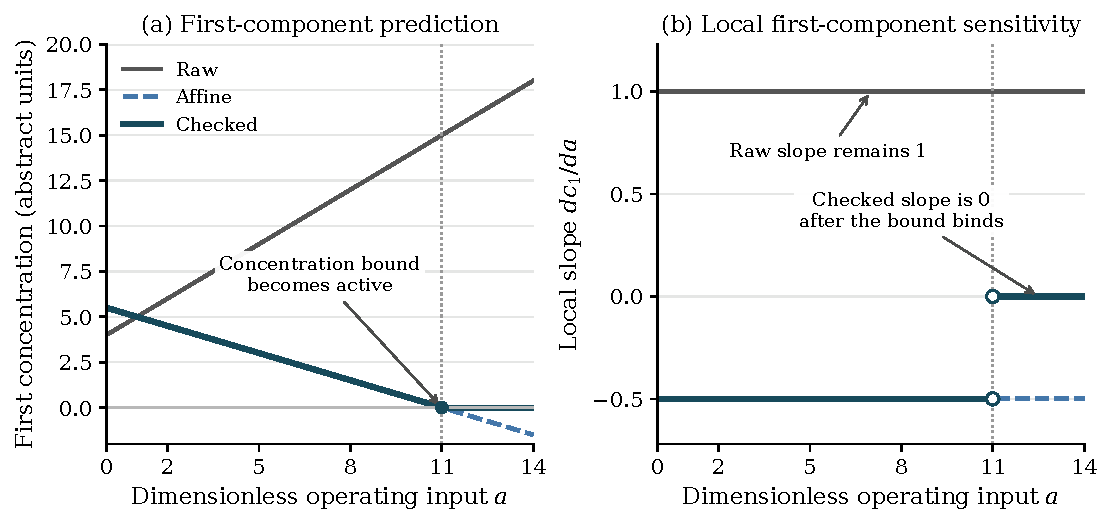
\includegraphics[width=\textwidth]{ch7_concept_branch_sensitivity.pdf}
\caption{Hypothetical first-component response and sensitivity before and after mass conservation and non-negativity enforcement. Open circles mark the two one-sided checked slopes at the active-boundary transition.}
\label{fig:assessment_branch_sensitivity}
\end{figure}

Before the concentration boundary becomes active, the affine and checked responses coincide. Their negative first-component slope differs from the positive raw slope because mass conservation redistributes the operating response across the two components. After the boundary activates, the checked concentration remains at zero and its local slope becomes zero. The transition is therefore characterized by distinct one-sided sensitivities. This example summarizes why interpretation must follow the complete deployed calculation.

\subsection{Assessment design for the structured regression}

\subsubsection{Common inputs and comparator models}

The structured-regression assessment uses a design collection of 10,000 accepted steady-state reactor cases. Every predictor receives the same 22 physical inputs and targets the same 20 effluent components. COD, TN, TP, and TSS are subsequently calculated through the common composition matrix. The input domain, reaction model, simulation bounds, and acceptance criteria remain those of the declared reactor benchmark. The comparison therefore changes the statistical predictor while keeping the physical process and prediction task fixed.

The nine unconstrained comparators are XGBoost, LightGBM, CatBoost, AdaBoost, random forest, support vector regression, \(k\)-nearest neighbors, partial least squares, and a fully connected multilayer perceptron. Together, they represent boosted and randomized tree ensembles, kernel regression, local neighbor averaging, latent linear regression, and nonlinear neural regression. Their methodological foundations include the ensemble construction of \citet{Breiman2001}, the boosting formulations of \citet{Drucker1997}, \citet{ChenGuestrin2016}, \citet{Ke2017}, and \citet{Prokhorenkova2018}, and the latent regression framework of \citet{Wold2001}. These comparators do not use an invariant penalty, auxiliary non-negative fitted-state matrix, or learned component-coupling equation during fitting. The latent components of partial least squares are statistical combinations of the inputs rather than physical process components. The supervised target nevertheless remains the same 20-component effluent state for all methods.

The neural comparator uses hidden layers of 128, 64, and 32 units with logistic activation. Dense connections map the 22 inputs through these layers to the 20 component outputs. Its flexible internal representation is therefore compared with the explicit polynomial structure of ICSOR without changing the prediction target or reporting map.

\subsubsection{Training partitions and hyperparameter selection}

The primary assessment uses a row-wise 80\% training and 20\% held-out split with random seed 42. From the 10,000-case design, 8000 observations form the training pool and 2000 form the final held-out set. Hyperparameter selection uses only the training pool. Half of that pool forms a 4000-row tuning subset, which is further split into 3200 tuning-training and 800 tuning-validation observations.

Each predictor receives 100 hyperparameter trials under a seeded tree-structured Parzen estimator with seed 42. No trial pruning or wall-clock timeout is imposed. \citet{Bergstra2011} develop this search strategy, while \citet{Akiba2019} provide the associated hyperparameter optimization framework. The selection criterion is mean squared error in the shared physical component space on the internal validation set. Once selected, the settings are held fixed for the primary assessment and repeated sample-size study. The final primary model is then fitted using all 8000 training observations.

For the unconstrained comparators, input and output standardization parameters are estimated from the applicable training partition. Predictions are transformed back to physical component coordinates before invariant checking, reporting, or error assessment. ICSOR remains in physical coordinates throughout so that its coefficients, invariant operator, and deployment constraints share the same component convention. Internal-validation transformations are estimated only from the tuning-training rows. Thus, means, standard deviations, and hyperparameters are determined without access to the held-out test responses. Projection weights are likewise fixed before held-out assessment.

Table~\ref{tab:icsor_comparator_settings} lists the specified comparator configurations. These settings describe the fitted models and should not be interpreted as performance results.

\begin{table}[htbp]
\centering\small
\caption{Specified configurations of the nine unconstrained comparators.}\label{tab:icsor_comparator_settings}
\begin{tabular}{p{0.19\textwidth}p{0.74\textwidth}}
\toprule
Comparator & Configuration\\
\midrule
XGBoost & 309 trees, learning rate 0.125, maximum depth 3, minimum child weight 6.84, row fraction 0.915, feature fraction 0.828, absolute penalty \(1.18\times10^{-3}\), and squared penalty 0.382.\\
LightGBM & 302 trees, learning rate 0.0809, 16 leaves, maximum depth 8, minimum leaf count 14, row fraction 0.845, feature fraction 0.869, absolute penalty \(3.17\times10^{-3}\), and squared penalty \(3.36\times10^{-4}\).\\
CatBoost & 236 boosting iterations, learning rate 0.172, depth 4, leaf squared penalty 0.0266, bagging temperature 0.0277, and random strength 0.0657.\\
AdaBoost & 236 estimators, learning rate 0.999, and squared regression loss.\\
Random forest & 390 trees, maximum depth 14, minimum split count 3, minimum leaf count 1, feature fraction 0.500, and no bootstrap resampling.\\
Support vector regression & Polynomial kernel of degree 4, regularization parameter 0.118, insensitive-error width 0.0458, constant offset 0.889, and solver tolerance \(8.96\times10^{-4}\). The kernel scale is the reciprocal of the product of input dimension and training input variance.\\
\(k\)-nearest neighbors & 15 neighbors, inverse-distance weighting, Manhattan distance, and a k-dimensional search tree with leaf size 40.\\
Partial least squares & 6 latent components, maximum 887 fitting iterations, and tolerance \(9.91\times10^{-5}\).\\
Multilayer perceptron & Hidden widths \((128,64,32)\), logistic activation, adaptive moment estimation, squared penalty \(6.33\times10^{-4}\), batch size 64, initial learning rate \(1.08\times10^{-3}\), maximum 500 iterations, and tolerance \(1.63\times10^{-5}\). Training rows are not shuffled, and early stopping is disabled.\\
\bottomrule
\end{tabular}
\end{table}

\subsubsection{Scoring states and physical diagnostics}

The scored ICSOR prediction is its final checked component state. For comparator accuracy assessment, the raw comparator prediction receives the same affine mass-conservation projection in Equation~\eqref{eq:icsor_affine_solution}, after which the common reporting map is applied. The accuracy comparison therefore evaluates the checked structured prediction against comparator predictions aligned to the same invariant equalities. Comparator accuracy scoring uses the affine state, whereas ICSOR accuracy scoring uses the complete deployed state, including the constrained non-negativity projection when required.

The numerical assessment uses an operator \(A_{num}\) obtained by rounding the null-space basis, removing negligible coefficients, and dividing each row by its first nonzero coefficient. Fitting, affine projection, and constrained deployment use this numerical operator in place of the ideal operator \(A\). Reported balance violations therefore refer specifically to these adopted numerical relations and the stated scaling.

Physical diagnostics use the raw comparator predictions rather than their affine-aligned accuracy states. ICSOR diagnostics distinguish the raw coupled prediction, affine projection, and final deployed state. This separation makes it possible to identify which stage produces physical compliance. The empirical balance diagnostic is \(v_{mc}^{num}(c)=\|A_{num}(c-c_{in})\|_2\), while non-negativity is assessed using \(v_{nn}\) from Equation~\eqref{eq:icsor_deployment_diagnostics}. For either diagnostic,
\begin{equation}
\equationname{Percentage frequency of a physical-constraint violation}
\label{eq:icsor_violation_frequency}
f_v=\frac{100}{n}\sum_{i=1}^{n}
\mathbf{1}\{v(c_i)>10^{-10}\}.
\end{equation}
Violation frequencies, residual magnitudes, adjustment distances, and deployment-branch use answer different questions about the same prediction procedure. They are therefore reported alongside, rather than substituted for, predictive error.

\subsubsection{Composite error measures}

The five reported error measures summarize different aspects of predictive disagreement. Consider two hypothetical observations with reference values \((2,4)\) and predictions \((3,2)\). The residuals are \((1,-2)\), their squares are \((1,4)\), and their absolute values are \((1,2)\). The resulting mean squared error is 2.5, root mean squared error is approximately 1.5811, and mean absolute error is 1.5.

The corresponding absolute relative errors are \(1/2\) and \(2/4\), giving a mean relative absolute error of 0.5. The reference mean is 3, with total squared variation \((2-3)^2+(4-3)^2=2\). The prediction residual squared sum is 5, so \(R^2=1-5/2=-1.5\). The negative value indicates that the hypothetical prediction has greater squared error than using the reference mean for both observations. These calculations illustrate why the metrics provide complementary information.

For reported quantity \(q\in\{1,2,3,4\}\), let \(e_{iq}=\widehat y_{iq}-y_{iq}\). The squared, root, and absolute measures are
\begin{equation}
\equationname{Per-composite squared, root, and absolute error measures}
\label{eq:icsor_composite_error_metrics}
E_{2,q}=\frac{1}{n}\sum_i e_{iq}^{2},
\qquad E_{root,q}=\sqrt{E_{2,q}},
\qquad E_{1,q}=\frac{1}{n}\sum_i|e_{iq}|.
\end{equation}
For strictly nonzero reference values,
\begin{equation}
\equationname{Mean relative absolute error of a reported composite}
\label{eq:icsor_relative_error}
E_{rel,q}=\frac{1}{n}\sum_i\frac{|e_{iq}|}{|y_{iq}|}.
\end{equation}
The quantity is reported as a ratio; multiplying by 100 gives a percentage. A zero reference value makes the expression undefined, while a very small reference can make the relative error disproportionately large. Any convention for zero-reference cases must therefore be defined before predictors are compared.

The target-specific coefficient of determination is
\begin{equation}
\equationname{Coefficient of determination for a reported composite}
\label{eq:icsor_coefficient_determination}
R_q^2=1-
\frac{\sum_i e_{iq}^{2}}
{\sum_i(y_{iq}-\overline y_q)^2}.
\end{equation}
A target with no reference variation makes the expression undefined. Negative values are possible when the prediction error exceeds that of the reference-mean predictor.

The aggregate root error pools residuals across the four reported quantities:
\begin{equation}
\equationname{Root mean squared error pooled across four reported composites}
\label{eq:icsor_aggregate_root_error}
E_{root}=\left(\frac{1}{4n}\sum_{q=1}^{4}\sum_{i=1}^{n}e_{iq}^{2}\right)^{1/2}.
\end{equation}
Aggregate absolute and relative errors use the corresponding means across observations and reported quantities, while aggregate \(R^2\) is the mean of the four target-specific coefficients. Because the composite coordinates retain their own physical units, the pooled error is a benchmark summary under that numerical convention rather than a dimensionless measure. Per-target scores remain necessary to identify which reported quantities drive the aggregate.

Pooling before taking the square root is also distinct from averaging target-specific root errors. If four hypothetical target mean squared errors are 1, 9, 1, and 9, the pooled mean squared error is 5 and the pooled root error is \(\sqrt5\approx2.2361\). The average of the four target root errors is instead \((1+3+1+3)/4=2\). Equation~\eqref{eq:icsor_aggregate_root_error} defines the first of these two summaries.

The primary ordering measure is aggregate root mean squared error. The remaining measures provide complementary perspectives: squared error emphasizes large residuals, absolute error describes average deviation, relative error scales that deviation to the reference magnitude, and \(R^2\) relates squared error to target variation. Predictor rankings are therefore examined separately under each measure.

\subsubsection{Repeated sample-size assessment}

The sample-size assessment uses
\begin{equation}
\equationname{Observation counts for structured-regression sample-size assessment}
\label{eq:icsor_assessment_sizes}
n\in\{500,1450,2400,3350,4300,5250,6200,7150,8100,9050,10000\}.
\end{equation}
At each size, ten subsamples are drawn without replacement from the design collection using deterministic seeds derived from 42. Each subsample receives an 80\% training and 20\% held-out split, and all ten predictors use the same sampled rows and partitions. The complete design therefore contains 110 fits per predictor.

The selected hyperparameters remain fixed across this assessment. This isolates the effect of data availability under a common model specification rather than allowing each sample size to define a new tuned model. Mean held-out scores and their variability are summarized across the ten runs. These learning curves show how the relative value of model flexibility and structural constraints changes with the simulation budget \citep{Geman1992,VieringLoog2023}.

The learning-curve area can be understood from a reduced example. Suppose an error measure takes values 6, 4, and 3 at sample sizes 100, 200, and 400. The first trapezoid has width 100 and average height 5, giving area 500. The second has width 200 and average height 3.5, giving area 700. The total area is therefore 1200. Dividing by the complete width \(400-100=300\) gives a normalized area of 4. Wider sample-size intervals contribute proportionally more to this average.

For retained sizes \(n_1,\ldots,n_S\), the numerical approximation is
\begin{equation}
\equationname{Trapezoidal approximation of normalized learning-curve area}
\label{eq:icsor_learning_area_trapezoids}
\frac{1}{n_{max}-n_{min}}
\sum_{s=1}^{S-1}(n_{s+1}-n_s)
\frac{\overline M_{m,j}(n_s)+\overline M_{m,j}(n_{s+1})}{2}.
\end{equation}
The corresponding continuous definition is
\begin{equation}
\equationname{Integral definition of normalized learning-curve area}
\label{eq:icsor_learning_area}
L_{m,j}=\frac{1}{n_{max}-n_{min}}
\int_{n_{min}}^{n_{max}}\overline M_{m,j}(n)\,\mathrm{d}n.
\end{equation}
Here \(\overline M_{m,j}(n)\) is the mean held-out value of measure \(j\) for predictor \(m\) at sample size \(n\). Dividing by the sample-size interval makes the result an average curve height and preserves the units of the original measure. \citet{Cawley2011} and \citet{Guyon2011} provide related trajectory summaries in active learning, while the present study varies the number of randomly sampled training observations.

Ranks provide a separate view of relative ordering. If four hypothetical errors are 3.0, 3.0, 4.5, and 6.0, their dense ranks are 1, 1, 2, and 3. The tie receives the same rank, and the next distinct score receives the next consecutive rank. The numerical distance between 4.5 and 6.0 does not affect the difference between their ranks.

For each measure \(j\), reported quantity \(q\), and retained sample size \(n_s\), predictors receive a dense rank \(r_{m,j,q}(n_s)\) based on their mean held-out score. Lower squared, root, absolute, and relative errors receive better ranks, whereas larger \(R^2\) values receive better ranks. With \(S=11\) sizes and five measures,
\begin{equation}
\equationname{Mean dense ranks over quantities, measures, and sample sizes}
\label{eq:icsor_dense_rank}
\overline r_{m,j}=\frac{1}{4S}\sum_{q=1}^{4}\sum_{s=1}^{S}r_{m,j,q}(n_s),
\qquad
\overline r_m=\frac{1}{5}\sum_{j=1}^{5}\overline r_{m,j}.
\end{equation}
These summaries describe relative performance over the declared comparisons. \citet{Demsar2006} develops broader rank-based model comparisons, while \citet{Shevchenko2024} emphasize the importance of benchmarking variability. Absolute error and mean rank are therefore reported together so that ordering is not detached from error magnitude.

At the largest sample size, the generalization gap is
\begin{equation}
\equationname{Held-out minus training root-error gap}
\label{eq:icsor_generalization_gap}
\Delta E_{root,m}=E_{root,m}^{held\text{-}out}-E_{root,m}^{training}.
\end{equation}
A positive value indicates greater held-out error. The gap does not by itself measure predictive quality: a model can have a small gap because it performs similarly well on training and held-out data, or because it performs similarly poorly on both. For example, training and held-out errors of 0.5 and 0.8 give a gap of 0.3, while errors of 5.0 and 5.1 give a smaller gap of 0.1 despite much worse prediction. The gap is therefore interpreted together with the absolute error \citep{Hastie2009}.

Training time is recorded for every repeated fit and summarized across runs. Deployment effort is assessed separately through prediction time, branch use, and constrained-solve effort. This separation distinguishes the cost of constructing the approximation from the cost of returning a physically checked state.

\subsection{Interpretability assessment}

The interpretability assessment examines the six driver blocks, the coupling matrix, and the corresponding raw component and composite mappings. It asks what the fitted structure reveals about the response within the declared process domain. \citet{Brunton2016} connect interpretable nonlinear terms to the broader problem of recovering mathematical structure from data, while \citet{Machado2014} show how operational and influent uncertainty complicate interpretation in activated sludge systems.

The driver and coupling parameters can trade off in the simultaneous relation \(Rc=B\phi\). Different joint stationary solutions can therefore produce similar component predictions using different coefficient allocations \citep{Selerio2026}. The imposed symmetry removes one source of redundancy in the ordered quadratic terms, but it does not establish unique causal parameter identification. Coefficient signs and magnitudes are therefore interpreted together with the complete fitted response rather than in isolation.

Prediction error and physical diagnostics are also separated across the raw regression, affine projection, and final deployed state. This distinction makes clear what the statistical model learns and what the projection subsequently imposes \citep{Karniadakis2021,KircherVotsmeier2025}. Projection magnitude is examined because a final state can satisfy the adopted constraints while remaining far from the raw prediction. Likewise, fitting effort and deployment effort are recorded separately because they represent different computational costs.

The assessment is therefore limited to steady-state component prediction within the stated input domain and control volume. The raw regression provides an inspectable statistical approximation. Checked deployment then imposes the adopted numerical invariants and non-negativity requirements on the returned state.

\section{Results}
\label{sec:icsor_results}

\subsection{Accuracy on the fixed held-out partition}

Table~\ref{tab:icsor_fixed_results} summarizes predictive performance on the 2000 fixed held-out cases. ICSOR is evaluated using its final checked state, while the comparator predictions are evaluated after affine alignment to the adopted mass conservation relations. The multilayer perceptron produced the lowest pooled root mean squared error at 4.38, followed by LightGBM at 5.30. Support vector regression and ICSOR were closely spaced at 5.97 and 5.98, respectively. Under the pooled native composite-coordinate convention of Equation~\eqref{eq:icsor_aggregate_root_error}, ICSOR therefore provided competitive but not leading full-data accuracy.

\begin{table}[htbp]
\centering\small
\caption{Fixed-split held-out composite performance. ICSOR is scored after checked deployment. Comparators are scored after affine alignment without a non-negativity constraint. Relative absolute error is a ratio rather than a percentage.}
\label{tab:icsor_fixed_results}
\begin{tabular}{p{4.7cm}rrrr}
\toprule
Predictor & $E_{root}$ & $E_1$ & Mean $R^2$ & $E_{rel}$\\
\midrule
Multilayer perceptron & 4.38 & 2.55 & 0.9915 & 0.0123\\
LightGBM & 5.30 & 3.21 & 0.9806 & 0.0203\\
Support vector regression & 5.97 & 3.49 & 0.9713 & 0.0244\\
ICSOR & 5.98 & 3.70 & 0.9700 & 0.0256\\
XGBoost & 6.12 & 3.81 & 0.9733 & 0.0244\\
CatBoost & 6.45 & 4.07 & 0.9727 & 0.0250\\
AdaBoost & 21.27 & 13.15 & 0.8643 & 0.0653\\
$k$-nearest neighbors & 23.61 & 13.87 & 0.8535 & 0.0557\\
Partial least squares & 28.24 & 17.05 & 0.7808 & 0.0681\\
Random Forest & 29.00 & 16.93 & 0.7934 & 0.0632\\
\bottomrule
\end{tabular}
\end{table}

Relative to the two leading predictors, ICSOR's pooled root error was 36.5\% higher than that of the multilayer perceptron and 12.8\% higher than that of LightGBM. It nevertheless remained slightly below XGBoost and CatBoost on the same measure. Its mean absolute relative error of 0.0256 corresponds to 2.56\%. The fixed-split comparison therefore quantifies the predictive cost associated with using the more structured model under the largest-data setting.

Figure~\ref{fig:icsor_fixed_results} shows the same comparison for pooled root error, pooled absolute error, and mean composite \(R^2\). ICSOR ranked fourth by pooled root error on this partition, reinforcing the conclusion that its principal advantage at the largest design size is not minimum error alone.

\begin{figure}[htbp]
\centering
\includegraphics[width=\textwidth]{results/ch5/q01_fixed_split_accuracy.png}
\caption{Fixed-split composite accuracy on 2000 held-out cases. Teal bars identify ICSOR after checked deployment. Gray bars identify comparators after affine alignment. Pooled root and absolute errors retain the native composite-coordinate convention. The right panel averages four composite-specific $R^2$ values.}
\label{fig:icsor_fixed_results}
\end{figure}

The aggregate score also hides differences among the individual treatment quantities. Table~\ref{tab:icsor_target_results} separates COD, TN, TP, and TSS. ICSOR's COD root error was 7.77, only 0.18 above LightGBM and lower than that of the other non-neural predictors. Its TN and TSS errors were 3.55 and 8.36, respectively. The multilayer perceptron produced the lowest COD, TN, and TSS errors. All methods had the same TP error of 0.0361 after the specified alignment and reporting procedure, so TP did not distinguish the predictors in this comparison.

\begin{table}[htbp]
\centering\small
\caption{Fixed-split root mean squared error for each composite. COD, TN, TP, and TSS use g COD m$^{-3}$, g N m$^{-3}$, g P m$^{-3}$, and g TSS m$^{-3}$, respectively.}
\label{tab:icsor_target_results}
\begin{tabular}{p{4.7cm}rrrr}
\toprule
Predictor & COD & TN & TP & TSS\\
\midrule
Multilayer perceptron & 6.48 & 1.58 & 0.0361 & 5.66\\
LightGBM & 7.59 & 2.77 & 0.0361 & 6.85\\
Support vector regression & 8.87 & 3.50 & 0.0361 & 7.20\\
ICSOR & 7.77 & 3.55 & 0.0361 & 8.36\\
XGBoost & 8.78 & 3.27 & 0.0361 & 7.88\\
CatBoost & 9.13 & 3.23 & 0.0361 & 8.53\\
AdaBoost & 38.30 & 5.58 & 0.0361 & 17.68\\
$k$-nearest neighbors & 38.24 & 4.23 & 0.0361 & 27.37\\
Partial least squares & 43.22 & 5.09 & 0.0361 & 36.00\\
Random Forest & 45.87 & 4.00 & 0.0361 & 35.26\\
\bottomrule
\end{tabular}
\end{table}

Figure~\ref{fig:icsor_composite_results} makes the scale difference among these quantities visible. COD and TSS contributed much larger numerical errors to the pooled score than TP. The separate target panels are therefore necessary for interpreting what the aggregate comparison represents.

\begin{figure}[htbp]
\centering
\includegraphics[width=\textwidth]{results/ch5/q02_composite_accuracy.png}
\caption{Fixed-split root mean squared error for COD, TN, TP, and TSS. Teal identifies ICSOR and gray identifies the comparators. Each panel has its own constituent unit and horizontal scale. All methods have the same reported TP error under the specified alignment and reporting procedure.}
\label{fig:icsor_composite_results}
\end{figure}

\subsection{Sample efficiency and generalization}

The repeated sample-size assessment produced a different picture from the fixed large-data comparison. At the smallest design size of 500 cases, ICSOR had the lowest mean held-out root error at 10.79. XGBoost and LightGBM followed at 11.26 and 11.45, while the multilayer perceptron ranked fifth at 13.26. At the largest design size, however, the ordering changed: the multilayer perceptron reached 4.62, LightGBM 5.27, support vector regression 5.84, and ICSOR 5.94. The leading model therefore depended on the available simulation budget rather than remaining fixed across the learning curve.

\begin{table}[htbp]
\centering\small
\caption{Repeated-split composite assessment over eleven design sizes and ten runs per size. Final error and the held-out minus training gap refer to $n=10{,}000$. The learning-curve area is normalized by the design-size interval. Lower error and curve-area values indicate better performance. The gap measures the separation between training and held-out error.}
\label{tab:icsor_scaling_results}
\begin{tabular}{p{4.3cm}rrrr}
\toprule
Predictor & \begin{tabular}{r}Final\\$E_{root}$\end{tabular} & \begin{tabular}{r}Normalized\\curve area\end{tabular} & Mean rank & $\Delta E_{root}$\\
\midrule
Multilayer perceptron & 4.62 & 6.75 & 2.5 & 0.65\\
LightGBM & 5.27 & 6.35 & 2.2 & 1.99\\
Support vector regression & 5.84 & 6.90 & 4.0 & 1.19\\
ICSOR & 5.94 & 6.33 & 4.3 & 0.22\\
XGBoost & 6.10 & 7.01 & 4.3 & 1.44\\
CatBoost & 6.26 & 7.60 & 5.0 & 0.69\\
AdaBoost & 21.42 & 20.29 & 8.2 & 0.23\\
$k$-nearest neighbors & 23.76 & 25.77 & 7.0 & 23.66\\
Partial least squares & 27.96 & 30.17 & 9.4 & 0.38\\
Random Forest & 28.78 & 30.31 & 8.2 & 18.71\\
\bottomrule
\end{tabular}
\end{table}

Across the complete range of design sizes, ICSOR had the lowest normalized root-error curve area at 6.33. LightGBM was nearly identical at 6.35 and achieved the best mean dense rank of 2.2. The multilayer perceptron had the second-best mean rank at 2.5, while ICSOR and XGBoost both had a mean rank of 4.3. These summaries emphasize different aspects of performance: the curve area favors sustained low root error across the data range, whereas the rank aggregates relative ordering across targets, metrics, and sizes. ICSOR therefore led one trajectory summary without leading all comparative summaries.

Its training-to-held-out behavior also differed from that of the more flexible learners. At the largest design size, ICSOR's held-out minus training root-error gap was 0.22, smaller than the corresponding gaps for the multilayer perceptron, LightGBM, XGBoost, and support vector regression. Partial least squares also had a small gap of 0.38, but its held-out root error was 27.96. A small gap alone therefore did not imply useful prediction. ICSOR combined a small gap with substantially lower absolute error than partial least squares, while the most accurate flexible learners still achieved lower final prediction error.

Figure~\ref{fig:icsor_efficiency_results} separates the normalized curve area, mean dense rank, and final generalization gap. The figure reinforces that no single summary dominates the interpretation: ICSOR led the root-error area, LightGBM led the mean-rank comparison, and the absolute held-out error remained necessary for interpreting the generalization gap.

\begin{figure}[htbp]
\centering
\includegraphics[width=\textwidth]{results/ch5/q03_sample_efficiency.png}
\caption{Normalized root-error curve area, mean dense rank, and held-out minus training root-error gap. Curve areas and ranks summarize eleven design sizes with ten repeated splits per size. The gap refers to the largest design size. Teal identifies ICSOR. The gap is reported alongside the held-out error.}
\label{fig:icsor_efficiency_results}
\end{figure}

The change in model ordering is especially clear at the two endpoints shown in Figure~\ref{fig:icsor_budget_results}. ICSOR led the four selected predictors when only 500 cases were available, whereas the multilayer perceptron had the lowest error at 10,000 cases. The result therefore supports a conditional interpretation of the structured model: its advantage is strongest when simulation data are limited, while flexible nonlinear learners benefit more from the larger design.

\begin{figure}[htbp]
\centering
\includegraphics[width=\textwidth]{results/ch5/q04_data_budget_comparison.png}
\caption{Mean held-out pooled composite root error at design sizes 500 and 10,000 for ICSOR, XGBoost, LightGBM, and the multilayer perceptron. Values summarize ten repeated splits. The panels show repeated-split endpoint means at the two specified design sizes.}
\label{fig:icsor_budget_results}
\end{figure}

\subsection{Physical checks and deployment branches}

The physical diagnostics distinguish statistical prediction from the properties of the returned component state. Table~\ref{tab:icsor_physical_results} compares the final ICSOR output with the raw outputs of the nine comparators. Every final ICSOR state satisfied both the adopted numerical balances and non-negativity tolerance. By contrast, every raw comparator state violated the adopted balance tolerance. Several comparators---AdaBoost, random forest, and \(k\)-nearest neighbors---produced no negative raw states, but this did not make them mass conserving. For the remaining comparators, raw non-negativity violation rates ranged from 46.00\% to 70.10\%.

\begin{table}[htbp]
\centering\small
\caption{Component-state violation frequencies on the 2000 held-out cases. ICSOR uses its final checked state. Comparators use their raw state, not the affine-aligned state used for accuracy scoring. Balance violations refer to $A_{num}$ and the declared $10^{-10}$ tolerance.}
\label{tab:icsor_physical_results}
\begin{tabular}{p{5.2cm}rr}
\toprule
Predictor & Balance violations (\%) & Negative states (\%)\\
\midrule
Multilayer perceptron & 100.0 & 58.20\\
LightGBM & 100.0 & 46.00\\
Support vector regression & 100.0 & 68.65\\
ICSOR & 0.0 & 0.00\\
XGBoost & 100.0 & 64.95\\
CatBoost & 100.0 & 70.10\\
AdaBoost & 100.0 & 0.00\\
$k$-nearest neighbors & 100.0 & 0.00\\
Partial least squares & 100.0 & 48.70\\
Random Forest & 100.0 & 0.00\\
\bottomrule
\end{tabular}
\end{table}

The stage-wise ICSOR diagnostics show how this final compliance was obtained. None of the raw coupled predictions passed both physical checks because all violated the adopted balance tolerance, although 21.7\% were already non-negative. Affine projection restored the balance equalities in every case and simultaneously produced a non-negative state for 436 predictions, or 21.8\% of the held-out set. These states could be returned immediately. The remaining 1564 cases, or 78.2\%, required the weighted linear projection to enforce non-negativity while preserving the balances. That solve required a mean of 23.5 iterations and a maximum of 40. Every resulting final state passed both checks.

Figure~\ref{fig:icsor_deployment_results} separates the raw comparator diagnostics from the internal stages of ICSOR deployment. This separation is essential because the final zero-violation result was not a property of the raw regression. It was produced by the projection procedure. The affine stage supplied balance compliance, while the constrained linear projection supplied the additional correction needed for most cases to satisfy non-negativity.

\begin{figure}[htbp]
\centering
\includegraphics[width=\textwidth]{results/ch5/q05_physical_deployment.png}
\caption{Physical diagnostics and ICSOR deployment on 2000 held-out cases. The left panel compares final ICSOR states with raw comparator states. The middle panel separates raw coupled, affine, and final ICSOR compliance. The right panel gives the numbers returned after affine projection and after constrained linear projection. Balance checks use the adopted numerical operator $A_{num}$.}
\label{fig:icsor_deployment_results}
\end{figure}

The branch counts therefore identify the source of physical admissibility. Fitting guidance alone did not make the raw state compliant. The affine projection restored the adopted invariant relations, and the constrained projection handled the remaining concentration violations. The complete checked deployment procedure, rather than the regression by itself, produced the zero final violation rates.

\subsection{Computational effort}

The structured fitting procedure required more computation than the fastest comparators, but its relative cost changed with the design size. At 500 cases, mean ICSOR fitting time was 21.5 s, compared with 4.72 s for LightGBM, 3.16 s for XGBoost, and 4.99 s for the multilayer perceptron. At 10,000 cases, ICSOR required 94.4 s. LightGBM and the other fast tree ensembles remained much faster, while partial least squares and \(k\)-nearest neighbors required only 0.228 and 2.70 s, respectively.

ICSOR was nevertheless not the slowest model at the largest design size. Its mean fitting time remained below AdaBoost at 117.7 s, support vector regression at 136.8 s, and the multilayer perceptron at 161.6 s. The result places the structured fit between the fastest conventional regressors and several computationally heavier nonlinear alternatives.

Fitting time is only one part of the computational requirement. Most fixed-split ICSOR predictions also required constrained deployment: the linear projection branch was activated in 78.2\% of cases. The reported iteration counts therefore represent additional repeated-use effort beyond the raw regression evaluation. Separating fitting from deployment makes clear that model preparation and physically checked prediction impose different computational costs.

Figure~\ref{fig:icsor_fitting_results} shows the fitting-time comparison on logarithmic axes. The smaller-design panel focuses on four leading predictors, while the larger-design panel includes additional alternatives. The figure therefore describes model-construction effort only; projection and checked deployment are accounted for separately.

\begin{figure}[htbp]
\centering
\includegraphics[width=\textwidth]{results/ch5/q06_fitting_effort.png}
\caption{Mean fitting times for the specified predictors at design sizes 500 and 10,000. Teal identifies ICSOR. Each panel uses a logarithmic seconds axis. The values concern repeated model fits and exclude deployment calculations.}
\label{fig:icsor_fitting_results}
\end{figure}

\subsection{Inspectable coefficient structure}

The fitted coefficient structure shows where ICSOR remained selective and where it relied on dense dependence among component channels. Table~\ref{tab:icsor_coefficient_results} reports the COD raw-composite polynomial coefficients together with the shared coupling matrix. The polynomial representation contains 276 unique candidate terms. Adding the 380 off-diagonal coupling entries gives 656 entries in the displayed structure. Under the specified post-fitting thresholds, 469 entries were retained, corresponding to 71.5\% of the combined display.

\begin{table}[htbp]
\centering\small
\caption{Coefficients exceeding the reporting thresholds in one fitted model. Polynomial blocks describe the COD row of $B_{\mathrm{raw,comp}}$. The coupling matrix is shared across component outputs and uses its own threshold. Symmetric quadratic blocks count unique upper-triangular terms.}
\label{tab:icsor_coefficient_results}
\begin{tabular}{p{6.2cm}rrr}
\toprule
Coefficient block & Candidates & Retained & Retained (\%)\\
\midrule
Baseline $b$ & 1 & 1 & 100.0\\
Operating terms $W_u$ & 2 & 2 & 100.0\\
Influent terms $W_{in}$ & 20 & 19 & 95.0\\
Operating curvature $\Theta_{uu}$ & 3 & 3 & 100.0\\
Operating-load interactions $\Theta_{uc}$ & 40 & 29 & 72.5\\
Influent curvature $\Theta_{cc}$ & 210 & 44 & 21.0\\
Shared off-diagonal coupling $\Gamma$ & 380 & 371 & 97.6\\
Combined display & 656 & 469 & 71.5\\
\bottomrule
\end{tabular}
\end{table}

The contrast between influent curvature and component coupling was pronounced. Only 44 of 210 unique influent-curvature terms exceeded the display threshold, whereas 371 of 380 coupling entries did. The fitted representation was therefore selective in its nonlinear influent curvature but dense in the dependence learned among output components. This pattern is important for interpretation because it shows that the visible polynomial structure was not uniformly sparse.

The largest absolute COD influent-curvature coefficient was the dissolved-oxygen self term at \(-5.8097\). The two mirrored dissolved-oxygen--dinitrogen entries were each \(-1.7411\), giving a combined unordered interaction coefficient of \(-3.4822\). Other prominent terms linked dissolved oxygen with metal phosphate, ammonia-oxidizing biomass, soluble phosphate, nitrite-oxidizing biomass, and nitrite. These coefficients belong to the raw COD composite mapping after both component coupling and reporting have been applied.

Figure~\ref{fig:icsor_structure_results} shows the retained counts and selected oxygen-related curvature terms. The plotted interaction values combine the two mirrored cells, consistent with the symmetry convention. The figure therefore describes the fitted polynomial in its native input units rather than implying that coefficient magnitudes from different units are directly comparable.

\begin{figure}[htbp]
\centering
\includegraphics[width=\textwidth]{results/ch5/q07_coefficient_structure.png}
\caption{Coefficient structure of one fitted ICSOR model. The left panel separates entries above and below the display thresholds for the COD polynomial blocks and shared coupling. The right panel shows selected COD influent-curvature coefficients with mirrored interaction entries combined. Coefficient units depend on the corresponding input terms. The displayed values describe the raw composite mapping.}
\label{fig:icsor_structure_results}
\end{figure}

\section{Discussion}
\label{sec:icsor_discussion}

\subsection{A structured approximation under limited data}

The results show that the value of the structured model depends strongly on the available data budget. ICSOR produced the lowest mean held-out root error at the smallest design size and the lowest normalized root-error curve area across the full sample-size range. Its explicit second-order driver, invariant-aware fitting objective, and learned component coupling therefore provided a useful approximation when fewer mechanistic simulations were available. This behavior is consistent with the broader role of model structure in hybrid learning discussed by \citet{Shen2023} and with the changing learner orderings across data budgets reviewed by \citet{VieringLoog2023}.

That advantage did not persist as a universal ranking. At the largest design size, the multilayer perceptron produced the lowest composite error, while LightGBM achieved the best mean dense rank across targets, metrics, and sample sizes. ICSOR's normalized curve area of 6.33 was only slightly lower than LightGBM's 6.35, but its final full-data error remained higher than that of the strongest flexible learners. The result therefore does not support choosing ICSOR simply because it is interpretable. Instead, it identifies a specific trade-off: ICSOR offers an explicit equation, favorable performance when simulations are limited, and checked component states, while more flexible learners can achieve lower prediction error when a larger training design is available \citep{Rudin2019,BhosekarIerapetritou2018}.

The generalization results reinforce the same point. ICSOR's training-to-held-out root-error gap was small, but a small gap is useful only when the underlying prediction error is also acceptable. Partial least squares demonstrated the opposite case: it also had a relatively small gap, yet its held-out error remained high. The leading flexible learners achieved lower absolute error despite larger training-to-held-out differences. Generalization gap and predictive accuracy therefore describe complementary properties and should not be interpreted as substitutes for one another.

From an engineering perspective, the sample-size results provide a practical model-selection rule rather than a universal ranking. When generating mechanistic training cases is costly and only a modest design can be afforded, the structured response can make efficient use of those cases while retaining direct inspectability. When simulation data are abundant and minimum predictive error is the dominant requirement, the results favor the more flexible learners evaluated here. The usefulness of an interpretable surrogate therefore depends on the data available and on whether transparency and physical checking are themselves required properties of the engineering workflow.

\subsection{Fitting guidance and final-state enforcement}

The physical results clarify the different roles of fitting guidance and output enforcement. The invariant penalty influenced the auxiliary training states, and the learned coupled system produced the raw prediction for a new input. Neither step, however, guaranteed that the raw deployed state satisfied the adopted physical requirements. Every raw ICSOR prediction in the fixed held-out set required at least the affine mass-conservation projection.

Projection then supplied the guarantees that fitting alone did not provide. The affine stage restored the adopted balances for every held-out case and was sufficient to return a non-negative state for 21.8\% of the predictions. The remaining 78.2\% required the weighted constrained projection, after which every returned state satisfied both the balance and non-negativity checks. The final zero-violation result is therefore attributable to the checked deployment procedure rather than to the soft penalty used during model fitting. This separation is consistent with the distinction between physics-guided learning and explicit output enforcement examined by \citet{Hansen2024} and \citet{KircherVotsmeier2025}.

This distinction is important because a physically checked output is not the same as a statistically superior output. The same deployment procedure that guarantees the adopted balances can alter concentrations and therefore alter prediction error. The numerical comparison used checked ICSOR states and affine-aligned comparator states for accuracy scoring, while the physical comparator diagnostics intentionally used the raw comparator states. Under this convention, ICSOR had a 36.5\% larger pooled root error than the multilayer perceptron, and all methods shared the same TP error of 0.0361 after alignment and reporting. These outcomes should therefore be read together with the deployment rules that produced them.

The result also shows why physical diagnostics need to identify the stage being assessed. A raw prediction, an affine mass-conserving state, and a jointly constrained final state are different mathematical objects. Reporting only the final zero-violation rate would hide how much correction was required to obtain it. Conversely, reporting only raw violations would ignore the state that the model actually returns to the engineer. The stage-wise analysis makes both facts visible: the statistical model frequently required correction, and the complete deployed procedure successfully supplied that correction.

\subsection{What the coefficient structure explains}

The fitted coefficient blocks make the response more inspectable by separating operating dependence, influent dependence, curvature, operating-load interactions, and component coupling. This explicit organization follows the preference for transparent predictive structures emphasized by \citet{Rudin2019}. It also prevents a regression coefficient from being interpreted outside the calculation in which it operates. A coefficient belongs first to the driver, after which coupling and the reporting map can redistribute its effect across component and composite outputs.

The fitted structure was not uniformly sparse. Most unique influent-curvature terms fell below the display threshold, while almost every off-diagonal coupling coefficient exceeded its separate threshold. The displayed model therefore combined selective nonlinear dependence on the influent with dense learned dependence among effluent components. The 469 retained entries out of 656 displayed candidates describe this contrast, but the threshold itself does not alter the fitted model. It only controls which coefficients are made visible in the summary.

The prominent oxygen-related terms provide a useful example of how the structure can be interpreted without claiming causal parameter identification. Oxygen availability is central to nitrification and interacts with other nutrient-removal pathways \citep{StenstromSong1991,Wentzel1992}. The dissolved-oxygen self term and the oxygen--dinitrogen interaction therefore identify fitted response patterns that can be compared with known process behavior. Their signs and magnitudes remain properties of the statistical mapping in its native units, not estimates of kinetic constants.

The sensitivity analysis extends this interpretation beyond coefficient inspection. A coefficient describes one term in the polynomial, but the local response at an operating point combines linear effects, curvature, interactions, component coupling, and physical projection. The analytical raw Jacobians in Equation~\eqref{eq:icsor_raw_jacobians} include the first three of these stages, while Equation~\eqref{eq:icsor_affine_jacobians} shows how mass conservation modifies those derivatives. The frequent activation of the constrained branch means that active-set effects are also relevant for many final predictions.

Figure~\ref{fig:assessment_branch_sensitivity} demonstrates why this distinction matters. In the illustrative response, a positive raw first-component slope became negative after affine mass-conservation projection and then became zero when the non-negativity boundary activated. A reader who inspected only the raw polynomial coefficient would therefore describe a different local response from the one returned by the deployed model. The interpretability contribution of ICSOR lies in making this entire sequence traceable.

\subsection{Engineering implications}

Taken together, the results define the engineering role of the structured surrogate more clearly than any single accuracy score. ICSOR combined competitive composite prediction, favorable behavior when training data were limited, an explicit response structure, and final component states that satisfied the imposed numerical checks. Its second-order terms and coupling matrix allow an engineer to examine how operating and loading conditions enter the fitted response. Checked deployment then ensures that COD, TN, TP, and TSS are calculated from a component state that satisfies the adopted material accounting and non-negativity requirements.

These benefits are accompanied by computational costs. ICSOR required more fitting time than the fastest tree and linear comparators, although at 10,000 cases it remained faster than AdaBoost, support vector regression, and the multilayer perceptron. More importantly, fitting time does not describe the full cost of using the model. Most fixed-split predictions required the constrained deployment solve after the raw regression had already been evaluated. The computational value of the model must therefore be assessed through both preparation and repeated deployment rather than through regression evaluation alone. This distinction follows the broader surrogate-modeling emphasis on separating model-development cost from repeated-use cost \citep{BhosekarIerapetritou2018,Bliek2023}.

The practical value of ICSOR is therefore conditional rather than absolute. It is not the most accurate predictor at the largest data budget, nor is its raw prediction automatically physically admissible. Its value is that the complete procedure exposes the fitted relationships, identifies where coupling and projection alter those relationships, and returns a component state that passes the declared physical checks. When transparency, limited simulation data, and component-level physical accounting are important, those properties provide engineering criteria that are not captured by prediction error alone.

The broader implication is that interpretability and physical consistency should be treated as properties of the complete deployed calculation. An explicit equation does not remain fully interpretable if later coupling and projection are ignored, and a physically constrained output does not become accurate merely because its balances close. The structured framework makes these distinctions explicit. It allows prediction accuracy, model structure, physical enforcement, and computational effort to be examined together without treating any one of them as evidence for the others.

\subsection{Data Availability}
\label{sec:icsor_data_availability}

The simulation data and numerical results supporting this study are publicly available at \url{https://github.com/egbertoselerio1997/icsor}.
\chapter{Connected plant surrogates and operating optimization}
\label{ch:plant}

\section{Rationale}

Activated sludge process optimization concerns the response of a connected treatment system rather than an isolated effluent prediction. Biological reactors transform material, secondary clarification separates solids, and recycle streams return material to earlier treatment locations. Mixed liquor contains both wastewater constituents and suspended biomass. Clarifier overflow carries treated water from the system, while underflow supplies concentrated sludge for return and wasting. The concentrations and flow rates of these streams determine how much material is discharged, circulated, retained, and removed. Aeration, recycle, and wasting therefore influence both final effluent quality and the solids inventory maintained within the plant \citep{Henze2008,HartelPopel1992}.

Mechanistic plant models provide the physical basis for representing these connections. The benchmark of \citet{Alex2008} links biological reactors, secondary clarification, internal recycle, return sludge, and wasting within one treatment system. The component-transport analysis of \citet{JeppssonDiehl1996} further shows why clarifier outlets must retain a consistent biological composition. At the reactor scale, the structured prediction of \citet{Selerio2026} provides an inspectable approximation at a single treatment boundary. The first gap addressed in this chapter is therefore how to extend component prediction and physical enforcement from one reactor to shared streams and stored solids across a connected plant. Accurate or physically checked predictions at individual units do not, by themselves, establish consistency among those units.

The return-sludge connection illustrates this problem directly. A predicted underflow concentration re-enters the mixer through the return flow. If the mixer prediction implies a different contribution from the same stream, the two outputs represent different amounts of the same transported material. Both predictions can remain non-negative while their connection is physically inconsistent. Clarifier storage introduces an additional requirement because retained solids contribute to the plant inventory and determine solids retention time. A connected plant response must therefore retain internal concentrations, separator outlets, and stored solids rather than reduce the treatment system to final-effluent totals alone \citep{Alex2008,JeppssonDiehl1996}.

Joint projection provides a way to reconcile these quantities simultaneously. Its effect, however, must be evaluated at the treatment locations where the predictions will actually be used. An adjustment that reconciles recycle and separator balances may also alter internal biomass, nutrient concentrations, and final effluent quality. Location-specific errors, physical residuals, and computational effort are therefore all needed to assess the connected prediction. At the same time, satisfaction of the selected flow, inventory, and concentration constraints does not establish agreement with every nonlinear reaction or settling equation. Physical enforcement guarantees only the relations that are explicitly imposed \citep{KircherVotsmeier2025,Selerio2026}.

The second gap concerns the operating decision obtained from this connected response. Surrogates can reduce the computational effort required for repeated process evaluations \citep{McBride2019,BhosekarIerapetritou2018}. The simulation-based search of \citet{Fang2011} and the resource-recovery framework of \citet{Durkin2024} illustrate how learned models can support wastewater treatment decisions. Yet agreement over a holdout design does not guarantee agreement at the operating settings preferred by an optimizer. Search naturally concentrates evaluations in regions that appear favorable. If treatment is predicted too optimistically in such a region, the resulting error can influence the selected capacity, aeration, recycle, or wasting settings even when average prediction error over the broader domain is small.

Independent evaluation of selected controls is therefore a separate requirement. The surrogate comparisons of \citet{Pedrozo2025} distinguish predictive accuracy from optimization behavior, while the approximation-management methods of \citet{Hameed2026} retain checks against the original model. These contributions motivate evaluating the mechanistic plant response at the controls selected by each optimization route. The relevant evidence includes the resulting effluent concentrations, the objective calculated on a common reference basis, and satisfaction of the original engineering requirements. The availability of a candidate decision and the numerical certification of the search are also different outcomes. Failed searches must remain visible when the practical usefulness of a route is assessed.

The meaning of an operating comparison also depends on the priorities embedded in its objective. \citet{Araujo2013} examine constrained economic operation, while \citet{PadronPaez2020} and \citet{Aboagye2021} connect treatment performance with resource use. Two optimization routes can therefore prefer different controls because one accepts greater resource demand to obtain better treatment. A meaningful comparison must use common priorities, common control bounds, and common mechanistic evaluation. It should also separate treatment-quality and resource contributions so that the source of a lower objective remains visible. A lower objective is a result under the declared preferences; it does not imply that every effluent quantity or every resource demand is lower.

Capacity selection is particularly important in the present study. At fixed fresh-influent flow, changing HRT changes the biological reactor volume. The resulting problem therefore combines capacity selection with aeration, recycle, and wasting decisions. It is not equivalent to adjusting the operation of an installed plant whose tanks are already fixed. The resource terms used below are engineering proxies for comparing the declared alternatives rather than measured electricity bills or full facility costs. These boundaries define the practical meaning of the optimization results and prevent a numerical objective from being interpreted as a demonstrated field saving.

This chapter addresses the fourth research question in Section~\ref{sec:research_questions}. The connected surrogate is termed Extended ICSOR. The direct route solves a smooth nonlinear programming (NLP) problem and is termed Smooth NLP. Their selected controls are compared through independent mechanistic evaluation and a common engineering objective. The contribution is a joint component-state formulation that connects physical enforcement with explicit decision verification. The assessment separates network consistency, prediction accuracy, selected treatment outcomes, search reliability, and computational effort. This separation identifies where rapid approximation can support plant analysis and where mechanistic evaluation remains necessary.

\section{Theory}

\subsection{Hydraulic connections and reactor inventories}

\subsubsection{Flow through the treatment train}

Let $Q_0$ denote the fresh-influent flow in m$^3$ d$^{-1}$ and let $c_{\rm in}\in\mathbb R_+^F$ denote its component concentrations. The plant has $n_r$ completely mixed reactors and an $L$-layer clarifier. Reactor concentrations are $c_1,\ldots,c_{n_r}$, the mixer concentration is $m$, and clarifier overflow and underflow concentrations are $c_E$ and $c_U$. Because the overflow is the final treated-water outlet, $c_{\rm out}=c_E$.

The dimensionless ratios $r_I$, $r_R$, and $w$ describe mixed-liquor recycle, return activated sludge, and waste activated sludge flow relative to $Q_0$. Mixed-liquor recycle leaves the final reactor before the clarifier. Return sludge and waste sludge both leave through the clarifier underflow and therefore share the same underflow concentration. Each ratio is an actual flow divided by $Q_0$. Denote the reactor-train, clarifier-feed, underflow, and overflow flows by $Q_P,Q_C,Q_U,Q_E$. The mixer, reactor splitter, underflow splitter, and external water balance give
\begin{align}
\equationname{Reactor-train flow including both recycle streams}
Q_P&=Q_0+r_IQ_0+r_RQ_0,\\
\equationname{Clarifier-feed flow after mixed-liquor recycle withdrawal}
Q_C&=Q_P-r_IQ_0,\\
\equationname{Clarifier underflow split into return sludge and waste sludge}
Q_U&=r_RQ_0+wQ_0,\\
\equationname{Effluent flow after waste withdrawal}
Q_E&=Q_0-wQ_0.
\end{align}
The second equation removes the mixed-liquor recycle before clarification, while the third collects both destinations of the clarifier underflow. Dividing each balance by $Q_0$ gives
\begin{equation}
\equationname{Plant flow ratios relative to fresh-influent flow}
q_P=1+r_I+r_R,\qquad q_C=1+r_R,\qquad
q_U=r_R+w,\qquad q_E=1-w.
\label{eq:plant_flows}
\end{equation}
Here $q_P$ is the reactor-train flow ratio and $q_C$ is the clarifier-feed flow ratio. The identity $q_C=q_E+q_U$ confirms the clarifier water balance. The adopted domain requires $r_I\ge0$, $r_R\ge0$, $0\le w<1$, and $q_U>0$, which ensures that the outlet concentrations are defined by positive outlet flows.

Figure~\ref{fig:plant_configuration} places these balances on the physical connections of a plant with $n_r$ reactors and $L$ clarifier layers. The case-study counts and aeration assignments are introduced in Methodology. The two recycle streams return material to the mixer, whereas treated water and waste sludge cross the external plant boundary.

\begin{figure}[htbp]
\centering
\resizebox{\linewidth}{!}{%
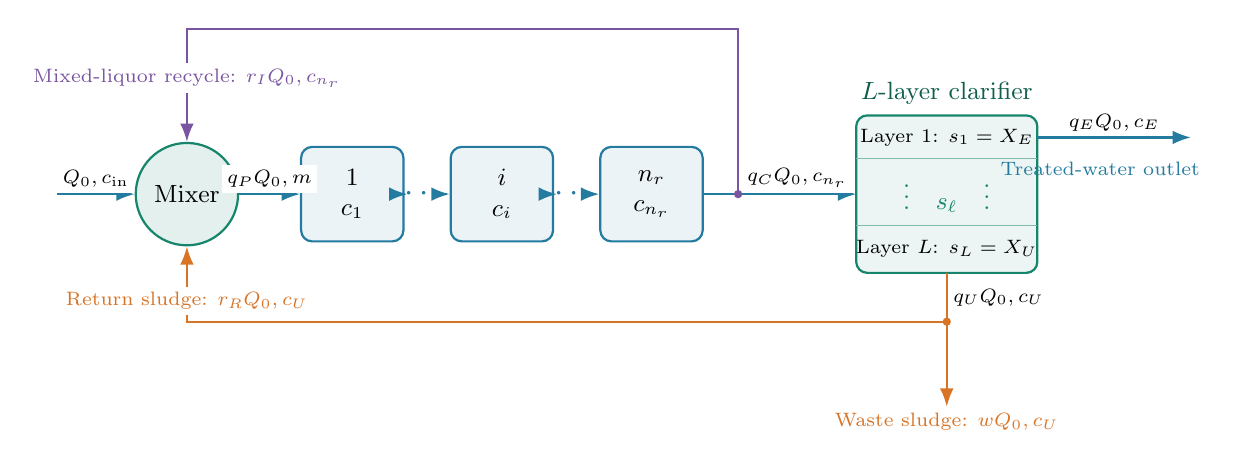
\begin{tikzpicture}[>=Latex,
unit/.style={draw=plantblue,fill=plantblue!9,rounded corners,minimum width=13mm,minimum height=12mm,align=center,font=\small,thick},
flow/.style={->,thick,draw=plantblue},lab/.style={font=\scriptsize,fill=white,inner sep=2pt}]
\node[draw=plantteal,fill=plantteal!12,circle,minimum size=13mm,thick,font=\small] (mix) at (0,0) {Mixer};
\node[unit] (r1) at (2.1,0) {$1$\\$c_1$};
\node[unit] (ri) at (4.0,0) {$i$\\$c_i$};
\node[unit] (rn) at (5.9,0) {$n_r$\\$c_{n_r}$};
\node[font=\large,text=plantblue] at (3.05,0) {$\cdots$};
\node[font=\large,text=plantblue] at (4.95,0) {$\cdots$};
\coordinate (split) at (7.0,0);
\draw[draw=plantteal,fill=plantteal!8,rounded corners,thick] (8.5,-1.0) rectangle (10.8,1.0);
\node[font=\small,text=plantteal!70!black] at (9.65,1.28) {$L$-layer clarifier};
\draw[draw=plantteal!55] (8.5,.45)--(10.8,.45);
\draw[draw=plantteal!55] (8.5,-.4)--(10.8,-.4);
\node[font=\scriptsize] at (9.65,.72) {Layer $1$: $s_1=X_E$};
\node[font=\small,text=plantteal] at (9.65,.05) {$\vdots\quad s_\ell\quad\vdots$};
\node[font=\scriptsize] at (9.65,-.70) {Layer $L$: $s_L=X_U$};
\draw[flow] (-1.65,0)--(mix.west) node[midway,above,lab] {$Q_0,c_{\rm in}$};
\draw[flow] (mix.east)--(r1.west) node[midway,above,lab] {$q_PQ_0,m$};
\draw[flow] (r1.east)--(2.80,0);
\draw[flow] (3.30,0)--(ri.west);
\draw[flow] (ri.east)--(4.70,0);
\draw[flow] (5.20,0)--(rn.west);
\draw[thick,draw=plantblue] (rn.east)--(split);
\draw[flow] (split)--(8.5,0) node[midway,above,lab] {$q_CQ_0,c_{n_r}$};
\fill[plantpurple] (split) circle (1.5pt);
\draw[->,thick,draw=plantpurple] (split)--(7.0,2.1)--(0,2.1)--(mix.north)
node[pos=.58,above,lab,text=plantpurple] {Mixed-liquor recycle: $r_IQ_0,c_{n_r}$};
\draw[flow] (10.8,.72)--(12.75,.72) node[midway,above,lab] {$q_EQ_0,c_E$};
\node[font=\scriptsize,text=plantblue] at (11.60,.32) {Treated-water outlet};
\coordinate (underflow) at (9.65,-1.62);
\draw[thick,draw=plantorange] (9.65,-1.0)--(underflow) node[midway,right,lab] {$q_UQ_0,c_U$};
\fill[plantorange] (underflow) circle (1.5pt);
\draw[->,thick,draw=plantorange] (underflow)--(9.65,-2.7)
node[below,lab,text=plantorange] {Waste sludge: $wQ_0,c_U$};
\draw[->,thick,draw=plantorange] (underflow)--(0,-1.62)--(mix.south)
node[pos=.48,below,lab,text=plantorange] {Return sludge: $r_RQ_0,c_U$};
\end{tikzpicture}}
\caption{Connected plant boundary with $n_r$ biological reactors and $L$ clarifier layers. Blue arrows show the treatment path, purple the mixed-liquor recycle, and orange the clarifier underflow split into return and waste sludge. Intermediate reactors and layers are omitted for clarity. All flow ratios use fresh-influent flow as their basis. The operating case study uses five reactors and ten layers; its aeration duties are specified in Methodology.}
\label{fig:plant_configuration}
\end{figure}

The configuration also explains why the reactor-train and clarifier-feed flows differ. Mixed-liquor recycle is withdrawn before the clarifier, whereas return sludge originates from the clarifier underflow. The two recycle streams therefore carry concentrations from different locations. The mixer balance must use each stream's own flow and concentration rather than assigning a single recycle concentration to both.

The mixer balance is written component by component rather than in terms of an aggregate water-quality quantity. For component $f$, incoming and outgoing mass rates satisfy
\begin{equation}
\equationname{Scalar mixer equation for one component}
Q_Pm_f=Q_0c_{{\rm in},f}+r_IQ_0c_{n_r,f}+r_RQ_0c_{U,f}.
\end{equation}
When the component basis is g m$^{-3}$, each product has units of g d$^{-1}$. Dividing first by $Q_0$ and then by $q_P$ gives
\begin{equation}
\equationname{Mixer concentration as a flow-weighted component average}
m_f=\frac{c_{{\rm in},f}+r_Ic_{n_r,f}+r_Rc_{U,f}}{1+r_I+r_R}.
\end{equation}
For two components, the same calculation is performed independently in each row,
\begin{equation}
\equationname{Illustrative two-component mixer matrix equation}
\begin{bmatrix}q_P&0\\0&q_P\end{bmatrix}
\begin{bmatrix}m_1\\m_2\end{bmatrix}
=\begin{bmatrix}c_{{\rm in},1}+r_Ic_{n_r,1}+r_Rc_{U,1}\\
c_{{\rm in},2}+r_Ic_{n_r,2}+r_Rc_{U,2}\end{bmatrix}.
\end{equation}
The complete component vector therefore satisfies
\begin{equation}
\equationname{Vector mixer equation for the complete component state}
q_Pm=c_{\rm in}+r_Ic_{n_r}+r_Rc_U.
\label{eq:plant_mixer}
\end{equation}
A high mixer concentration can consequently arise from internal circulation rather than from creation of an external pollutant load. The component-resolved framework of \citet{Zhang2026} similarly treats recirculation and discharge streams explicitly.

A hypothetical example makes the flow weighting and recycle effect concrete. Let $Q_0=10{,}000$ m$^3$ d$^{-1}$, $r_I=2$, $r_R=0.5$, and $w=0.02$. The resulting physical flows $Q_P,Q_C,Q_U,Q_E$ are 35{,}000, 15{,}000, 5{,}200, and 9{,}800 m$^3$ d$^{-1}$, respectively. For one particulate component, let the fresh-influent, final-reactor, and underflow concentrations be 200, 1{,}000, and 2{,}000 g m$^{-3}$. The mixer calculation is
\begin{align}
\equationname{Illustrative component inventory entering the mixer}
q_Pm_f&=200+2(1{,}000)+0.5(2{,}000)=3{,}200,\\
\equationname{Illustrative mixer concentration after flow normalization}
m_f&=3{,}200/3.5=914.29\ \mathrm{g\,m^{-3}}.
\end{align}
The three incoming physical mass rates are 2{,}000, 20{,}000, and 10{,}000 kg d$^{-1}$, whose sum equals the 32{,}000 kg d$^{-1}$ leaving the mixer. The mixer concentration exceeds the fresh-influent concentration because both recycle streams return concentrated material. The example therefore illustrates how internal circulation changes concentration without creating external mass.

The nominal stage HRT is defined on the fresh-flow basis. Because volume divided by flow has units of time, $V_i/Q_0$ is measured in days and multiplication by 24 converts it to hours. The actual flow through each reactor is $Q_P=Q_0q_P$, so the residence time during one passage through reactor $i$ is $V_i/Q_P$ \citep{Henze2008,Alex2008}. The inverse of this residence time is the dilution rate. With reactor volume $V_i$,
\begin{equation}
\equationname{Stage retention times and recycle-adjusted dilution rates}
h_i=\frac{24V_i}{Q_0},\qquad H=\sum_{i=1}^{n_r}h_i,\qquad
d_i=\frac{Q_0q_P}{V_i}=\frac{24q_P}{h_i}.
\label{eq:plant_residence}
\end{equation}
The quantities $h_i$ and $H$ are in hours, while $d_i$ is in d$^{-1}$. The actual residence time during one passage through stage $i$ is $h_i/q_P$. For a hypothetical plant with $H=24$ h, $r_I=2$, and $r_R=0.5$, the reactor-train flow ratio is 3.5, so the train residence time per passage is approximately 6.86 h. With equal reactor volumes, each stage then has a residence time per passage of about 1.37 h. The example shows why nominal HRT and recycle flow must be interpreted together.

Fixed stage fractions can be represented by $h_i=f_i^V H$, where $f_i^V>0$ and $\sum_i f_i^V=1$. The case study uses equal fractions. Varying $H$ at fixed $Q_0$ therefore varies the total biological reactor volume. The optimization consequently combines capacity selection with operating decisions. In an existing plant with fixed tank volumes, these volumes would instead be parameters and $H$ would no longer appear in the free-control vector.

Let $\vartheta$ collect only the settings that vary freely. A constant setting remains a model parameter because treating it as a varying regression coordinate would create a zero-variance feature. A carbon or chemical addition may also enter the control vector. If an addition is represented only by a source term, its carrier flow is assumed negligible. If the carrier flow is appreciable, it must be represented as an additional hydraulic stream and the downstream dilution rates must be revised accordingly.

\subsubsection{Biological conversion and non-negativity}

The reaction network uses the component and process model developed in Chapter~\ref{ch:foundations}. Its stoichiometric matrix is $\nu\in\mathbb R^{P\times F}$ and its process-rate vector in reactor $i$ is $\rho_i\in\mathbb R_+^P$. For component $f$, the dynamic balance is
\begin{equation}
\equationname{Dynamic reactor-stage equation for one component}
V_i\frac{dc_{i,f}}{dt}=Q_Pc_{i-1,f}-Q_Pc_{i,f}
+V_i\sum_{p=1}^{P}\nu_{pf}\rho_{i,p}+V_i\omega_i(e_{S_O})_f+V_i\xi_{i,f}.
\end{equation}
The reaction sum combines the contributions of all modeled processes. A negative $\nu_{pf}$ consumes component $f$, while a positive entry produces it. The oxygen selector equals one for the dissolved-oxygen component and zero elsewhere. At steady state, accumulation vanishes. Dividing the remaining equation by $V_i$ gives
\begin{equation}
\equationname{Steady-state reactor-stage equation for one component}
0=d_i(c_{i-1,f}-c_{i,f})+\sum_{p=1}^{P}\nu_{pf}\rho_{i,p}
+\omega_i(e_{S_O})_f+\xi_{i,f}.
\end{equation}
Collecting all $F$ component balances gives the vector reactor equation, with $c_0=m$,
\begin{equation}
\equationname{Vector reactor-stage equation with aeration and external additions}
0=d_i(c_{i-1}-c_i)+\nu^\top\rho_i(c_i,\vartheta)
+k_La_i(a_i)(S_O^*-c_{i,S_O})e_{S_O}+\xi_i(\vartheta).
\label{eq:plant_reactor}
\end{equation}
The vector $e_{S_O}$ selects dissolved oxygen, $S_O^*$ is the oxygen saturation concentration, and $\xi_i$ represents declared stage additions. Every term has units of component concentration per day. The treatment-model framework of \citet{Henze2006} separates hydraulic transport, stoichiometric conversion, and external sources in this manner.

Non-negativity is a physical property of the dynamic state. At a boundary where one component concentration is zero, the combined reaction and external-source terms must not direct that component into negative values. With non-negative inflow and a locally Lipschitz balance function defined on the boundary, this condition preserves the non-negative state space of the dynamic model \citep{Haddad2010}. Numerical acceptance therefore checks concentrations and reaction rates independently of the solver's stopping message.

The same requirement does not arise automatically in a statistical surrogate. A fitted quadratic equation may predict a negative concentration even when every training state is non-negative because polynomial regression imposes no sign restriction on new outputs. The work of \citet{KircherVotsmeier2025} addresses simultaneous mass conservation and non-negativity in kinetic surrogates. Both properties therefore require explicit treatment in the connected plant surrogate.

\subsubsection{Stage invariants and the external plant balance}

The role of mass conservation can first be seen in a simple two-component reaction. Suppose one component is converted into another without changing their combined amount. The corresponding stoichiometric and inventory rows are
\begin{equation}
\equationname{Illustrative stoichiometric matrix and normalized invariant row}
\nu=\begin{bmatrix}-1&1\end{bmatrix},\qquad
A=\frac1{\sqrt2}\begin{bmatrix}1&1\end{bmatrix}.
\end{equation}
The factor $1/\sqrt2$ normalizes the inventory row to unit length. The reaction contribution disappears under multiplication by $A$,
\begin{equation}
\equationname{Illustrative cancellation of the reaction contribution to an invariant}
A\nu^\top=\frac1{\sqrt2}\left[1(-1)+1(1)\right]=0.
\end{equation}
At an illustrative dilution rate of 2 d$^{-1}$, let the upstream concentrations be $(12,3)$ and the downstream concentrations be $(8,7)$ g m$^{-3}$, with a reaction rate of 8 g m$^{-3}$ d$^{-1}$. The two component balances are
\begin{align}
\equationname{Illustrative steady-state equation for the consumed component}
0&=2(12-8)-8,\\
\equationname{Illustrative steady-state equation for the produced component}
0&=2(3-7)+8.
\end{align}
Adding the balances removes the unknown reaction rate. Both upstream and downstream totals are 15 g m$^{-3}$, and the normalized invariant is that total divided by $\sqrt2$. The full reactor model applies the same cancellation principle to a larger set of components and processes.

Let $A\in\mathbb R^{K\times F}$ contain independent inventory rows satisfying
\begin{equation}
\equationname{Reaction, oxygen-forcing, and rank identities of the plant invariant operator}
A\nu^\top=0,\qquad Ae_{S_O}=0,\qquad
\operatorname{rank}(A)=K.
\label{eq:plant_invariant_operator}
\end{equation}
The rows are normalized to unit Euclidean length, although this normalization does not make them mutually orthogonal. Physically named inventories and an orthonormal basis can span the same mass-conservation subspace while using different coordinates. The stoichiometric fixed-layer formulation of \citet{SturmWexler2022} illustrates the usefulness of separating conserved inventories from the reaction rates that redistribute them.

For inventory row $k$, multiply component equation $f$ by $A_{kf}$ and sum over $f$. The reaction contribution becomes
\begin{equation}
\equationname{Scalar cancellation of reaction rates in an invariant equation}
\sum_{f=1}^{F}A_{kf}\sum_{p=1}^{P}\nu_{pf}\rho_{i,p}
=\sum_{p=1}^{P}\left(\sum_{f=1}^{F}A_{kf}\nu_{pf}\right)\rho_{i,p}=0.
\end{equation}
The inner sum is entry $(k,p)$ of $A\nu^\top$. Oxygen transfer likewise disappears because $Ae_{S_O}=0$. The remaining scalar relation is
\begin{equation}
\equationname{Scalar reactor-stage invariant equation with external additions}
d_i\left(\sum_fA_{kf}c_{i-1,f}-\sum_fA_{kf}c_{i,f}\right)
+\sum_fA_{kf}\xi_{i,f}=0.
\end{equation}
Rearranging the transport difference and dividing by the positive $d_i$ gives
\begin{equation}
\equationname{Invariant inventory change across one reactor stage}
A(c_i-c_{i-1})=d_i^{-1}A\xi_i(\vartheta).
\label{eq:plant_invariant_transition}
\end{equation}
When no stage addition is present, $Ac_i=Ac_{i-1}$. Thus nitrification may transfer nitrogen from ammonium to oxidized forms, and denitrification may transfer it to dissolved nitrogen gas, while the complete nitrogen inventory remains unchanged. A reported quantity that excludes dissolved nitrogen gas can decrease even though the mass-conservation inventory remains constant. The nutrient-form interpretation in \citet{USEPA2009} therefore supports examining individual species as well as aggregate reporting quantities.

The same example also shows why external additions must appear in the invariant relation. If component 1 receives an addition of 2 g m$^{-3}$ d$^{-1}$ while the same reaction rate is retained, the downstream concentrations become $(9,7)$. The two balances are $2(12-9)-8+2=0$ and $2(3-7)+8=0$. Their total increases by $2/2=1$ g m$^{-3}$. An invariant relation that forced zero change would incorrectly remove the material introduced by the dose.

Internal recycle streams disappear only after the complete plant balance is assembled. First sum the reactor-stage transitions. Every intermediate $Ac_i$ then appears once with a positive sign and once with a negative sign, giving
\begin{align}
\equationname{Accumulated invariant change across the reactor train}
A(c_{n_r}-m)&=\sum_i\frac{V_i}{Q_0q_P}A\xi_i,\\
\equationname{Reactor-train invariant equation and external-addition total}
q_PAc_{n_r}-q_PAm&=D_{\rm add},\qquad
D_{\rm add}=\sum_i\frac{V_i}{Q_0}A\xi_i.
\end{align}
Next multiply the mixer balance by $A$ and substitute it for $q_PAm$,
\begin{align}
\equationname{Reactor-train invariant equation after mixer substitution}
q_PAc_{n_r}&=Ac_{\rm in}+r_IAc_{n_r}+r_RAc_U+D_{\rm add},\\
\equationname{Invariant equation after cancellation of mixed-liquor recycle}
(q_P-r_I)Ac_{n_r}&=Ac_{\rm in}+r_RAc_U+D_{\rm add}.
\end{align}
Because $q_P-r_I=q_C$, the left-hand side is the clarifier-feed inventory flow. The clarifier balance provides a second expression for the same quantity,
\begin{equation}
\equationname{Clarifier-feed invariant flow equals the two outlet invariant flows}
q_CAc_{n_r}=q_EAc_E+(r_R+w)Ac_U.
\end{equation}
Equating the two expressions and subtracting $r_RAc_U$ cancels the return-sludge flow. Mixed-liquor recycle has already canceled through $q_P-r_I$. The remaining external plant balance is
\begin{equation}
\equationname{External plant mass conservation after internal recycle cancellation}
Ac_{\rm in}+\sum_{i=1}^{n_r}\frac{V_i}{Q_0}A\xi_i
=q_EAc_E+wAc_U.
\label{eq:plant_external_invariant}
\end{equation}
Only fresh feed, stage additions, final effluent, and waste sludge remain. The recycle ratios continue to influence the internal state and treatment performance, but their cancellation from the external balance confirms that they are internal transfers rather than external sources or sinks.

For ASM2d-TSN, $F=20$, $P=28$, and $K=5$. The five inventories represent soluble inert material, total nitrogen including dissolved nitrogen gas, total phosphorus, an alkalinity-related combination, and a metal-related combination. The last two unnormalized combinations are
\begin{align}
\equationname{Alkalinity-related invariant combination}
I_{\rm alk}&=S_{ALK}-\frac{S_{NH4}}{14}
+\frac{S_{NO2}}{14}+\frac{S_{NO3}}{14}-\frac{S_{PO4}}{31},\\
\equationname{Metal-related invariant combination}
I_{\rm metal}&=3.45X_{MeP}+4.87X_{MeOH}.
\label{eq:plant_named_invariants}
\end{align}
The nitrogen and phosphorus rows use the constituent weights in Table~\ref{tab:component_basis_composites}, and the nitrogen inventory assigns unit weight to dissolved nitrogen gas. Under the stated parameterization, the stoichiometric rank is 15. These inventory identities are audited directly rather than inferred from reporting labels such as TN.

\subsection{Clarification and solids storage}

\subsubsection{A nonreactive separator with two outlet flows}

The clarifier is represented as a nonreactive settling unit. In the adopted formulation, the clarifier transports and separates components but does not perform biological or chemical conversion. Soluble components follow the liquid phase, whereas particulate components can settle and become concentrated in the underflow. \citet{Takacs1991} provide the settling and thickening formulation used for the aggregate solids profile, while \citet{JeppssonDiehl1996} show why propagation of component composition through a clarifier requires more information than aggregate suspended-solids concentration alone.

Selection means extracting designated entries of a vector without altering their values. For the illustrative component order $(S_A,S_{NH4},X_H,X_I)$, define
\begin{equation}
\equationname{Illustrative soluble and particulate component selectors}
E_S=\begin{bmatrix}1&0&0&0\\0&1&0&0\end{bmatrix},\qquad
E_X=\begin{bmatrix}0&0&1&0\\0&0&0&1\end{bmatrix}.
\end{equation}
Then $E_Sc=(S_A,S_{NH4})^\top$ and $E_Xc=(X_H,X_I)^\top$. Transposing a selector places the selected entries back into their original positions while filling all other positions with zeros. In this example,
\begin{equation}
\equationname{Illustrative coordinate projectors from the component selectors}
E_S^\top E_S=\operatorname{diag}(1,1,0,0),\qquad
E_X^\top E_X=\operatorname{diag}(0,0,1,1).
\end{equation}
Their sum is the identity because every component belongs to exactly one group, and their cross-product is zero because the groups do not overlap. For the complete ordered model, $E_S=[I_{10}\ 0]$ and $E_X=[0\ I_{10}]$. More generally, let $E_S\in\mathbb R^{F_S\times F}$ and $E_X\in\mathbb R^{F_X\times F}$ select soluble and particulate components. They satisfy
\begin{equation}
\equationname{Completeness and orthogonality identities of the component selectors}
E_S^\top E_S+E_X^\top E_X=I_F,\qquad E_SE_X^\top=0.
\end{equation}
The column $t_X$ maps component concentrations to TSS. Its entries are non-negative and its soluble entries are zero.

For the four-component order above, $t_X=(0,0,0.90,0.75)^\top$. If $X_H=100$ and $X_I=40$ g COD m$^{-3}$, the resulting TSS concentration is $0.90(100)+0.75(40)=120$ g TSS m$^{-3}$. The coefficients convert the native COD-based component concentrations to suspended-solids mass. Adding the numerical concentrations directly would therefore calculate a different quantity.

For one component, clarifier mass conservation gives
\begin{equation}
\equationname{Scalar mass conservation across the clarifier}
Q_Cc_{n_r,f}=Q_Ec_{E,f}+Q_Uc_{U,f}.
\end{equation}
The statistical response stores component flows divided by $Q_0$,
\begin{equation}
\equationname{Flow-weighted clarifier outlet component responses}
g_E=q_Ec_E,\qquad g_U=q_Uc_U.
\label{eq:plant_outlet_flows}
\end{equation}
Because $q_E$ and $q_U$ are dimensionless, these coordinates have the same units as concentration. Their corresponding physical discharge rates are $Q_0g_E$ and $Q_0g_U$. Representing the outlet responses in this way avoids division by a potentially small underflow ratio inside the equality system. The complete component balance and soluble pass-through relations are
\begin{equation}
\equationname{Joint clarifier component and soluble-transport equalities}
g_E+g_U=q_Cc_{n_r},\qquad
E_Sg_U=q_UE_Sc_{n_r}.
\label{eq:plant_clarifier_equalities}
\end{equation}
Together, these equations imply $E_Sg_E=q_EE_Sc_{n_r}$. Settling therefore cannot directly remove a soluble nutrient in the adopted clarifier model.

For soluble component $f$, pass-through gives $c_{U,f}=c_{n_r,f}$. Substituting $g_{U,f}=q_Uc_{n_r,f}$ into the total component balance yields
\begin{align}
\equationname{Flow-weighted soluble component in the overflow}
g_{E,f}&=(q_C-q_U)c_{n_r,f}=q_Ec_{n_r,f},\\
\equationname{Equality of overflow and feed soluble concentrations}
c_{E,f}&=g_{E,f}/q_E=c_{n_r,f}.
\end{align}
For a hypothetical feed concentration of 20 g m$^{-3}$ and flow ratios $q_C=1.5$, $q_U=0.52$, and $q_E=0.98$, the feed, underflow, and overflow component flows are 30, 10.4, and 19.6 g m$^{-3}$ on the fresh-flow basis. Dividing by the respective outlet flow ratios recovers 20 g m$^{-3}$ in both outlets.

Particulate components instead satisfy the densification requirement
\begin{equation}
\equationname{Particulate densification requirement for the underflow}
E_Xg_U\ge q_UE_Xc_{n_r}.
\label{eq:plant_densification}
\end{equation}
After division by $q_U$, every underflow particulate concentration is at least as large as its feed concentration. Together with non-negative overflow and the total component balance, this relation also prevents the underflow from recovering more particulate material than enters the clarifier.

For an illustrative particulate component, take $q_C=1.5$, $q_U=0.52$, and a feed concentration of 100 g m$^{-3}$. Densification requires $g_U\ge52$ g m$^{-3}$ on the fresh-flow basis. Mass conservation and non-negative overflow require $g_U\le150$ g m$^{-3}$. The fraction of incoming particulate flow recovered in the underflow therefore lies between $0.52/1.5$ and one. A soluble component with the same feed concentration instead has $g_U=52$ and equal feed and outlet concentrations. These two cases clarify the different roles of the soluble and particulate constraints.

Choose, for example, an admissible particulate flow $g_U=140$. Mass conservation then gives $g_E=150-140=10$. Dividing by the respective flow ratios gives $c_U=140/0.52=269.23$ and $c_E=10/0.98=10.20$ g m$^{-3}$. The underflow has therefore recovered $140/150=93.33\%$ of the incoming component flow. This recovery cannot be inferred from concentration alone because the outlet water flows differ.

For any particulate component with positive feed concentration,
\begin{equation}
\equationname{Bounds on the fraction of feed particulate material recovered in underflow}
\frac{q_U}{q_C}\le\frac{g_{U,f}}{q_Cc_{n_r,f}}\le1.
\end{equation}
Because the TSS weights are non-negative, multiplication by $t_X$ preserves these inequalities. Hence $X_U\ge X_N$. The solids balance $q_CX_N=q_EX_E+q_UX_U$ then gives
\begin{equation}
\equationname{Overflow solids bound implied by particulate densification}
q_EX_E\le(q_C-q_U)X_N=q_EX_N.
\end{equation}
Division by $q_E>0$ establishes the corresponding overflow bound.

Applying $t_X$ gives the feed and outlet suspended-solids concentrations,
\begin{equation}
\equationname{Feed, overflow, and underflow suspended-solids concentrations}
X_N=t_X^\top c_{n_r},\qquad
X_E=\frac{t_X^\top g_E}{q_E},\qquad
X_U=\frac{t_X^\top g_U}{q_U}.
\label{eq:plant_tss_endpoints}
\end{equation}
The declared constraints imply $X_E\le X_N\le X_U$. These relations bound the direction of separation, but they do not determine its magnitude. Additional information is therefore required from either the nonlinear settling calculation or an empirical endpoint model.

\subsubsection{The layer-resolved mechanistic model}

The mechanistic clarifier resolves the solids profile across $L$ layers, numbered from the surface to the hopper. Their TSS concentrations are $s_1,\ldots,s_L$, with $s_1=X_E$ and $s_L=X_U$. The exact settling velocity at concentration $s$ is
\begin{equation}
\equationname{Bounded double-exponential settling velocity}
v(s,X_N)=\max\left\{0,\min\left[v_{\max},
v_0\left(e^{-r_h(s-f_{\rm ns}X_N)}-e^{-r_p(s-f_{\rm ns}X_N)}\right)\right]\right\}.
\label{eq:plant_settling_velocity}
\end{equation}
The gravitational solids flux is $sv(s,X_N)$. The nonsettleable fraction $f_{\rm ns}$ makes the settling offset depend on feed solids concentration. At an interface, a receiver concentration above $X_t$ activates a limitation by the smaller adjacent gravitational flux. Otherwise, the upper-layer gravitational flux passes to the receiver \citep{Takacs1991}. Hydraulic transport uses the overflow velocity above the feed layer and the underflow velocity below it.

Each finite-volume layer equation is formed as incoming solids flux minus outgoing solids flux, multiplied by $A_{\rm cl}/V_{{\rm cl},\ell}$. The feed layer additionally receives $Q_0q_CX_N/V_{{\rm cl},\ell_F}$. Internal interface fluxes cancel when the layer equations are summed. At steady state, the resulting total solids balance reduces to Equation~\eqref{eq:plant_clarifier_equalities} after application of $t_X$.

A three-layer example makes this cancellation explicit. Place the feed in layer 2, and let $B_{12}$ denote the net solids rate from layer 2 toward layer 1 and $B_{23}$ the net rate from layer 2 toward layer 3. These signed rates combine hydraulic and gravitational transport in g d$^{-1}$. The layer balances are
\begin{align}
\equationname{Illustrative solids equation for the upper clarifier layer}
V_1\dot s_1&=B_{12}-Q_Es_1,\\
\equationname{Illustrative solids equation for the clarifier feed layer}
V_2\dot s_2&=Q_CX_N-B_{12}-B_{23},\\
\equationname{Illustrative solids equation for the lower clarifier layer}
V_3\dot s_3&=B_{23}-Q_Us_3.
\end{align}
Adding the three equations eliminates both interface rates. At steady state, the remaining relation is $Q_CX_N=Q_EX_E+Q_UX_U$. The whole-clarifier balance therefore holds even though the internal interface fluxes depend nonlinearly on neighboring concentrations. Mass conservation alone cannot determine the internal fluxes or the shape of the layer profile.

At a mechanistic steady state, particulate outlet components are reconstructed using the final-reactor particulate composition,
\begin{equation}
\equationname{Particulate outlet reconstruction from endpoint solids concentrations}
E_Xc_E=\frac{s_1}{X_N}E_Xc_{n_r},\qquad
E_Xc_U=\frac{s_L}{X_N}E_Xc_{n_r}.
\label{eq:plant_outlet_reconstruction}
\end{equation}
Soluble outlet components remain equal to their feed concentrations. The mapping is defined for $X_N>0$ and assumes that the particulate composition leaving through the overflow and underflow retains the final-reactor composition \citep{JeppssonDiehl1996}.

\subsubsection{An exact interval for aggregate inventory under the endpoint envelope}

The clarifier inventory is the concentration in each layer multiplied by its volume and summed over the vessel. For an illustrative four-layer clarifier,
\begin{equation}
\equationname{Illustrative four-layer clarifier solids inventory}
M=V_1X_E+V_2s_2+V_3s_3+V_4X_U.
\end{equation}
If each layer has volume 100 m$^3$ and the concentrations are $(10,200,600,1{,}000)$ g m$^{-3}$, the total stored solids are $100(10+200+600+1{,}000)=181{,}000$ g, or 181 kg. For the general clarifier,
\begin{equation}
\equationname{General clarifier solids inventory and total volume}
M_{\rm cl}=\sum_{\ell=1}^{L}V_{{\rm cl},\ell}s_\ell,\qquad
V_{\rm cl}=\sum_{\ell=1}^{L}V_{{\rm cl},\ell}.
\label{eq:plant_inventory_definition}
\end{equation}
The outlet concentrations alone cannot determine this inventory because two clarifiers can share the same endpoints while storing different amounts internally. Whole-plant solids retention time therefore requires both the internal inventory and the solids leaving through the outlet streams. The benchmark formulation of \citet{Alex2008} likewise includes reactor and settler inventories in its sludge-age calculation.

The mechanistic acceptance envelope requires
\begin{equation}
\equationname{Interior-layer solids envelope between the outlet concentrations}
X_E\le s_\ell\le X_U,\qquad \ell=2,\ldots,L-1.
\label{eq:plant_layer_envelope}
\end{equation}
This condition constrains each interior layer between the two endpoint concentrations, but it does not require monotonic variation from one layer to the next. With positive layer volumes, the minimum inventory is obtained by assigning every interior layer $X_E$, while the maximum is obtained by assigning every interior layer $X_U$.

For four layers, the two unknown interior contributions satisfy
\begin{align}
\equationname{Lower inventory bound for two illustrative interior layers}
V_2X_E+V_3X_E&\le V_2s_2+V_3s_3\\
\equationname{Upper inventory bound for two illustrative interior layers}
&\le V_2X_U+V_3X_U.
\end{align}
Adding the fixed endpoint contributions gives
\begin{align}
\equationname{Lower total-inventory bound for an illustrative four-layer clarifier}
(V_1+V_2+V_3)X_E+V_4X_U&\le M,\\
\equationname{Upper total-inventory bound for an illustrative four-layer clarifier}
M&\le V_1X_E+(V_2+V_3+V_4)X_U.
\end{align}
For the hypothetical equal-volume clarifier above, these limits are 103{,}000 and 301{,}000 g, and the 181{,}000-g inventory lies within them. If the two internal concentrations were both 400 g m$^{-3}$, the total inventory would again be 181{,}000 g. Matching the endpoints and total inventory therefore does not uniquely determine the internal profile.

Figure~\ref{fig:plant_inventory_envelope} shows the same four-layer arithmetic as concentration bars. The surface and hopper concentrations remain fixed while the two internal layers change, altering the stored mass. The left and right panels attain the lower and upper inventory limits implied by the envelope.

\begin{figure}[htbp]
\centering
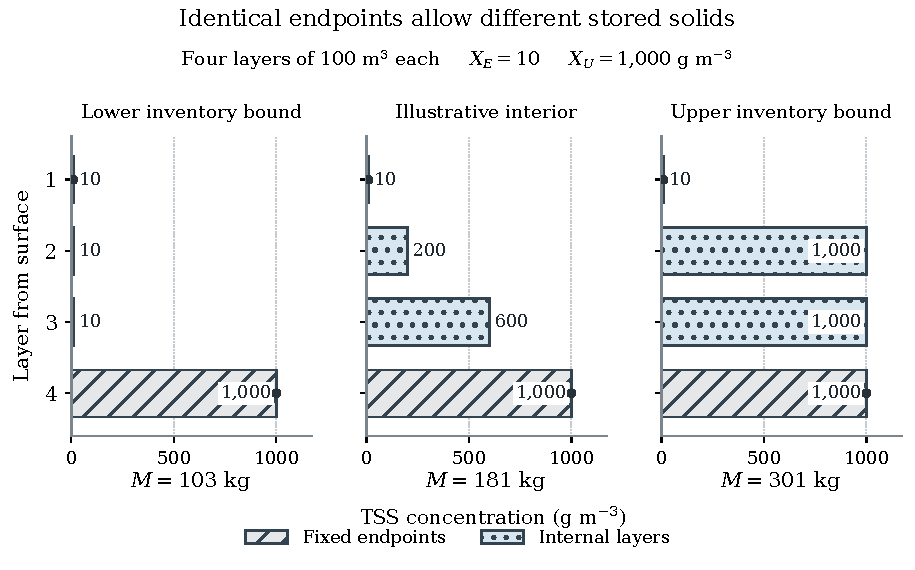
\includegraphics[width=\linewidth]{ch6_concept_inventory_envelope.pdf}
\caption{Hypothetical four-layer profiles with identical overflow and underflow concentrations. Each layer has volume 100 m$^3$. The lower-bound, illustrative interior, and upper-bound profiles store 103, 181, and 301 kg of solids. Hatching identifies the fixed endpoints, while dotted fills identify internal layers. The diagram represents the adopted endpoint envelope.}
\label{fig:plant_inventory_envelope}
\end{figure}

The middle profile is only one of many profiles that can share the same endpoints and total inventory. The scalar inventory retains the amount of stored solids, whereas the nonlinear layer equations provide the additional information needed to determine a mechanistic distribution.

For $L$ layers, the same argument replaces $V_2+V_3$ with $\sum_{\ell=2}^{L-1}V_{{\rm cl},\ell}$. Because this internal-volume sum is $V_{\rm cl}-V_{{\rm cl},1}-V_{{\rm cl},L}$, collecting endpoint coefficients gives
\begin{align}
\equationname{Lower clarifier-inventory bound from endpoint concentrations}
M_{\rm cl}^{-}&=(V_{\rm cl}-V_{{\rm cl},L})X_E+V_{{\rm cl},L}X_U,\\
\equationname{Upper clarifier-inventory bound from endpoint concentrations}
M_{\rm cl}^{+}&=V_{{\rm cl},1}X_E+(V_{\rm cl}-V_{{\rm cl},1})X_U,\\
\equationname{Admissible interval for the clarifier solids inventory}
M_{\rm cl}^{-}&\le M_{\rm cl}\le M_{\rm cl}^{+}.
\label{eq:plant_inventory_bounds}
\end{align}

These bounds are both necessary and sufficient for the existence of an endpoint-envelope profile with the stated total inventory. To see sufficiency, assign every interior layer a common concentration $s_*$ between $X_E$ and $X_U$. The total inventory becomes
\begin{equation}
\equationname{Inventory represented by a common interior-layer concentration}
V_{{\rm cl},1}X_E+V_{{\rm cl},L}X_U
+\left(V_{\rm cl}-V_{{\rm cl},1}-V_{{\rm cl},L}\right)s_*.
\end{equation}
As $s_*$ varies continuously between $X_E$ and $X_U$, this expression spans the entire admissible interval. For equal-volume layers, it also gives a simple constructive profile for every inventory admitted by the bounds.

As an illustrative calculation, consider ten layers of 600 m$^3$, with $X_E=10$ g m$^{-3}$ and $X_U=5{,}000$ g m$^{-3}$. The corresponding inventory interval is 3{,}054{,}000--27{,}006{,}000 g. Every inventory in this interval is compatible with at least one profile satisfying the endpoint envelope. Joint projection enforces this aggregate interval, whereas layer-resolved mechanistic evaluation checks the internal settling equations.

For the ten equal layers, the arithmetic is
\begin{align}
\equationname{Solids inventory of the illustrative ten-layer clarifier}
M_{\rm cl}&=600(X_E+s_2+s_3+\cdots+s_9+X_U),\\
\equationname{Lower inventory bound for the illustrative ten-layer clarifier}
M_{\rm cl}^{-}&=600(9X_E+X_U),\\
\equationname{Upper inventory bound for the illustrative ten-layer clarifier}
M_{\rm cl}^{+}&=600(X_E+9X_U).
\end{align}
At the lower endpoint, nine layers are at $X_E$ and one is at $X_U$; at the upper endpoint, one layer is at $X_E$ and nine are at $X_U$. This makes the coefficients in the compact interval physically transparent rather than treating them as fitted constants.

\subsection{Statistical prediction of the connected response}

\subsubsection{A response that preserves network and storage information}

The connected statistical response must retain enough information to reconstruct the physical relationships used in treatment and operating analysis. For a teaching example with one reactor and two components, let $S$ denote a soluble component and $X$ a particulate component. The stored response is the explicit nine-entry vector
\begin{equation}
\equationname{Illustrative joint response of a one-stage, two-component plant}
\chi_{\rm toy}=
(m_S,m_X,c_{1,S},c_{1,X},g_{E,S},g_{E,X},g_{U,S},g_{U,X},M_{\rm cl})^\top.
\end{equation}
Adding a second reactor inserts $c_{2,S}$ and $c_{2,X}$ before the outlet coordinates, increasing the vector length to eleven. In general, every reactor contributes $F$ component concentrations. The mixer and two clarifier outlets each contribute another $F$, and the clarifier inventory contributes one scalar. The connected surrogate therefore predicts
\begin{equation}
\equationname{Complete joint plant-response vector and its dimension}
\chi=\operatorname{col}(m,c_1,\ldots,c_{n_r},g_E,g_U,M_{\rm cl})
\in\mathbb R^{n_\chi},\qquad n_\chi=(n_r+3)F+1.
\label{eq:plant_joint_response}
\end{equation}
Here $\operatorname{col}$ stacks its arguments into one column. The response retains concentrations needed for reactor inventories, outlet flows needed for material balances, and clarifier storage needed for solids retention time. It intentionally omits the internal clarifier-layer profile. The full mechanistic state is
\begin{equation}
\equationname{Mechanistic reactor-and-clarifier state vector and its dimension}
y=\operatorname{col}(c_1,\ldots,c_{n_r},s_1,\ldots,s_L)
\in\mathbb R_+^{n_y},\qquad n_y=n_rF+L.
\label{eq:plant_mechanistic_state}
\end{equation}
The mapping from $y$ to $\chi$ deterministically reconstructs the mixer, both outlet streams, and the clarifier inventory. The reduced statistical response and the full mechanistic state therefore have different dimensions while still supporting the same engineering calculations.

For the five-reactor case, the connected response has $20+5(20)+20+20+1=161$ coordinates, whereas the full mechanistic state has $5(20)+10=110$. Table~\ref{tab:plant_response_positions} records the response ordering explicitly. A position identifies one coordinate and does not imply that neighboring coordinates have the same physical unit.

\begin{table}[htbp]
\centering\small
\caption{Blocks in the 161-coordinate connected response.}
\label{tab:plant_response_positions}
\begin{tabular}{lll}
\toprule Block & Positions & Coordinates\\\midrule
Mixer & 1--20 & $m_1,\ldots,m_{20}$\\
Reactor 1 & 21--40 & $c_{1,1},\ldots,c_{1,20}$\\
Reactor 2 & 41--60 & $c_{2,1},\ldots,c_{2,20}$\\
Reactor 3 & 61--80 & $c_{3,1},\ldots,c_{3,20}$\\
Reactor 4 & 81--100 & $c_{4,1},\ldots,c_{4,20}$\\
Reactor 5 & 101--120 & $c_{5,1},\ldots,c_{5,20}$\\
Overflow flows & 121--140 & $g_{E,1},\ldots,g_{E,20}$\\
Underflow flows & 141--160 & $g_{U,1},\ldots,g_{U,20}$\\
Clarifier inventory & 161 & $M_{\rm cl}$\\
\bottomrule
\end{tabular}
\end{table}

\subsubsection{Complete second-order features and ridge estimation}

The statistical input contains every free operating control together with every fresh-influent component concentration. Standardization first subtracts a fitting-set mean and divides by a fitting-set standard deviation. For one operating coordinate and one influent coordinate,
\begin{equation}
\equationname{Illustrative standardization of a control and an influent concentration}
z_1=\frac{\vartheta_1-\bar\vartheta_1}{s_{\vartheta_1}},\qquad
z_2=\frac{c_{{\rm in},1}-\bar c_{{\rm in},1}}{s_{{\rm in},1}}.
\end{equation}
The resulting coordinates are dimensionless. For hypothetical aeration $0.8$, fitting mean $0.5$, and fitting scale $0.1$, the standardized value is 3. For hypothetical ammonium concentration 40 g m$^{-3}$ with mean 30 and scale 10 g m$^{-3}$, the standardized value is 1. Standardization therefore prevents the regression penalty from being determined directly by the native units of the inputs. With fitting-set centers and positive diagonal scales,
\begin{equation}
\equationname{Standardized plant input vector and its dimension}
z=\operatorname{col}\left[D_{\vartheta,\rm fit}^{-1}(\vartheta-\bar\vartheta),
D_{{\rm in},\rm fit}^{-1}(c_{\rm in}-\bar c_{\rm in})\right]
\in\mathbb R^{d_z},\qquad d_z=d_\vartheta+F.
\label{eq:plant_standardized_input}
\end{equation}

For two standardized inputs, their symmetric product matrix is
\begin{equation}
\equationname{Illustrative quadratic product matrix of two standardized inputs}
zz^\top=\begin{bmatrix}z_1^2&z_1z_2\\z_2z_1&z_2^2\end{bmatrix}.
\end{equation}
Because multiplication commutes, $z_1z_2$ and $z_2z_1$ represent the same monomial. Keeping one triangular copy therefore yields the unique quadratic terms $(z_1^2,z_1z_2,z_2^2)$. Together with the intercept and two linear terms, this gives
\begin{equation}
\equationname{Illustrative unique-monomial second-order feature vector}
(1,z_1,z_2,z_1^2,z_1z_2,z_2^2)^\top.
\end{equation}
With three inputs, the feature vector contains an intercept, three linear terms, three squares, and three distinct cross-products, for ten features. In general, there are $d_z$ squares and $d_z(d_z-1)/2$ unique cross-products, giving
\begin{align}
\equationname{Linear and unique-quadratic feature coordinates}
r(z)&=\operatorname{col}\left[z,\operatorname{vech}(zz^\top)\right],\\
\equationname{Centered and scaled plant regression feature vector}
\phi(\vartheta,c_{\rm in})&=\operatorname{col}\left[1,D_{r,\rm fit}^{-1}(r(z)-\bar r)\right],\\
\equationname{Dimension of the unique-monomial plant feature vector}
n_\phi&=1+d_z+\frac{d_z(d_z+1)}{2}.
\label{eq:plant_features}
\end{align}
The operator $\operatorname{vech}$ keeps one triangular copy of the symmetric matrix, so every square and pairwise product appears once. A product between ammonium loading and aeration allows the aeration response to depend on influent loading, while a squared recycle term permits local curvature \citep{Nazlabadi2021,Selerio2026}. These features approximate the nonlinear input-response relation.

Quadratic features are themselves centered and scaled after construction. For the hypothetical standardized inputs $(3,1)$, the unscaled nonconstant terms are $(3,1,9,3,1)$. If the first squared feature has fitting mean 1 and standard deviation 2, its final value is $(9-1)/2=4$. If the cross-product has fitting mean 0.2 and standard deviation 0.5, its final value is $(3-0.2)/0.5=5.6$. This second stage of standardization prevents a feature with naturally large variance from receiving an effectively weaker ridge penalty simply because of its numerical scale \citep{Hastie2009}.

A monomial is one polynomial term, such as $z_1^2$ or $z_1z_2$. A feature set containing each distinct monomial once spans the same quadratic function family as an ordered set that includes both $z_1z_2$ and $z_2z_1$. The two duplicate coefficients enter prediction only through their sum. If the effective cross-product coefficient is $b$, the ordered representation can assign $b/2$ to each duplicate, producing a squared penalty of $b^2/2$ rather than $b^2$. Removing duplicate monomials therefore preserves the polynomial family but changes the regularization convention unless the penalty is adjusted. The connected fit selects its penalty for the stated feature family containing each distinct term once. With 27 inputs, the resulting feature count is $1+27+378=406$.

For response coordinate $k$, let its standardized target be $\widetilde\chi_{ik}=(\chi_{ik}-\bar\chi_k)/s_{\chi,k}$. Its fitted value is $C_{k0}+\sum_{j=1}^{n_\phi-1}C_{kj}\phi_{ij}$. The multiresponse ridge objective is
\begin{equation}
\equationname{Scalar expansion of the multiresponse ridge objective}
\frac1{n n_\chi}\sum_{i=1}^{n}\sum_{k=1}^{n_\chi}
\left(\widetilde\chi_{ik}-\sum_{j=0}^{n_\phi-1}C_{kj}\phi_{ij}\right)^2
+\frac{\gamma}{n_\chi}\sum_{k=1}^{n_\chi}\sum_{j=1}^{n_\phi-1}C_{kj}^2.
\end{equation}
The intercept corresponds to $j=0$. It appears in prediction but is excluded from the penalty. Dividing a physical prediction error by $s_{\chi,k}$ is equivalent to weighting its squared error by $1/s_{\chi,k}^2$. Response scaling therefore gives coordinates of different physical magnitudes comparable influence in the joint statistical score.

For example, an illustrative concentration error of 10 g m$^{-3}$ with response scale 20 g m$^{-3}$ contributes $0.5^2=0.25$ before averaging, whereas an inventory error of 10{,}000 g with scale 200{,}000 g contributes $0.05^2=0.0025$. Comparing the unscaled errors alone would suggest the opposite ordering. The fitted scales therefore define what constitutes a large error in the joint regression.

Let $\Phi_{\mathcal I}$ contain the feature rows for fitting indices $\mathcal I$, and let $\widetilde Y_{\mathcal I}$ contain the standardized joint responses. With $R_\phi=\operatorname{diag}(0,1,\ldots,1)$, the coefficient matrix solves
\begin{equation}
\equationname{Matrix form of the multiresponse ridge fitting problem}
\widehat C_\gamma=\arg\min_C
\left\{\frac{\|\widetilde Y_{\mathcal I}-\Phi_{\mathcal I}C^\top\|_F^2}
{|\mathcal I|n_\chi}+\frac{\gamma}{n_\chi}\|CR_\phi\|_F^2\right\}.
\label{eq:plant_ridge_fit}
\end{equation}
The intercept remains unpenalized. Positive $\gamma$ stabilizes the fit in the presence of correlated quadratic features. \citet{Hastie2009} describe this trade-off between flexibility and coefficient shrinkage. The raw prediction on the physical response scale is
\begin{equation}
\equationname{Raw joint plant prediction on the physical response scale}
\chi_{\rm raw}=\bar\chi+D_\chi\widehat C_\gamma\phi(\vartheta,c_{\rm in}).
\label{eq:plant_raw_prediction}
\end{equation}
The fixed response scale $D_\chi$ places inventory, concentration, and outlet-flow coordinates on comparable statistical scales. The joint projection described below then adjusts this raw response to satisfy the declared physical requirements.

For one response coordinate with coefficient vector $\beta$, differentiation of the scalar ridge objective gives the normal equations
\begin{equation}
\equationname{Normal equations for one ridge response coordinate}
(\Phi^\top\Phi+n\gamma R_\phi)\widehat\beta=\Phi^\top\widetilde\chi.
\end{equation}
The term $n\gamma R_\phi$ adds positive curvature to the nonintercept coefficient directions. A simple one-feature example illustrates the resulting shrinkage. Let three feature and target values both be $(-\sqrt{3/2},0,\sqrt{3/2})$, giving zero means and unit population standard deviations. Symmetry gives a zero intercept. With slope $b$, the objective becomes $(1-b)^2+\gamma b^2$. Differentiation gives $2(b-1)+2\gamma b=0$, so $\widehat b=1/(1+\gamma)$. For $\gamma=1$, the fitted slope is 0.5 rather than the unpenalized value of one.

Finally, the physical prediction is recovered coordinate by coordinate as $\chi_{{\rm raw},k}=\bar\chi_k+s_{\chi,k}\sum_j\widehat C_{kj}\phi_j$. A hypothetical mean of 100 g m$^{-3}$, scale of 20 g m$^{-3}$, and standardized prediction of 0.5 therefore return 110 g m$^{-3}$. Conversion back to physical units is required before component balances can be imposed.

The quadratic feature family is retained from ICSOR \citep{Selerio2026}. Its coefficients describe the raw statistical mapping. When projection is active, however, a raw coefficient is not generally the derivative of the final projected response because the projected derivative also depends on the constraints, their dependence on the controls, and the active inequality set.

\subsubsection{A separate positive model for overflow solids}

Overflow TSS occupies a much smaller concentration range than reactor solids, so its prediction requires particular care. An absolute error of 1 g m$^{-3}$ is only 1\% of 100 g m$^{-3}$ but 100\% of 1 g m$^{-3}$. A standardized joint-response score may therefore describe reactor and outlet solids adequately in aggregate while still obscuring relative error at the discharge point. The relative-error argument of \citet{Tofallis2015} motivates a separate logarithmic model for overflow solids.

For positive mechanistic targets, define
\begin{equation}
\equationname{Dimensionless logarithmic overflow-solids target}
\ell_E=\log(X_E/X_\star),\qquad X_\star=1\ \mathrm{mg\,L^{-1}}.
\label{eq:plant_log_target}
\end{equation}
The ratio inside the logarithm is dimensionless. The scalar ridge fit uses the same complete quadratic feature map,
\begin{equation}
\equationname{Ridge fitting problem for the logarithmic overflow model}
\widehat\beta_{E,\gamma_E}=\arg\min_\beta
\left\{\frac{\|\ell_{E,\mathcal I}-\Phi_{\mathcal I}\beta\|_2^2}{|\mathcal I|}
+\gamma_E\|R_\phi\beta\|_2^2\right\}.
\end{equation}
Its back-transformed prediction is
\begin{equation}
\equationname{Positive overflow-solids prediction from logarithmic back-transformation}
\widehat X_{E,\log}=X_\star\exp\left(\widehat\beta_{E,\gamma_E}^\top\phi\right)>0.
\label{eq:plant_log_prediction}
\end{equation}
A twofold concentration error therefore produces the same logarithmic discrepancy at low and high concentrations. Exponentiation also guarantees a positive statistical endpoint before the joint mass-conservation projection is solved.

A small example clarifies the interpretation of the logarithmic fit. For hypothetical targets of 2 and 8 mg L$^{-1}$, the dimensionless logarithms are $\log2$ and $\log8$. If one fitted log value represents them equally under squared logarithmic error, the minimizer is
\begin{equation}
\equationname{Illustrative logarithmic average and geometric concentration mean}
\frac{\log2+\log8}{2}=\log4.
\end{equation}
Back-transformation gives 4 mg L$^{-1}$, the geometric rather than arithmetic mean. A fitted log value of $-2$ gives 0.1353 mg L$^{-1}$, which is still positive even though it lies below $X_\star$. The reference concentration supplies units; it does not impose a lower concentration bound.

Under squared logarithmic error, direct exponentiation represents a conditional geometric center rather than an unbiased concentration-scale mean \citep{Tofallis2015}. No concentration-scale bias adjustment is therefore applied. The separate model also avoids imposing a constant solids-removal fraction across all influents and controls, which would ignore variation in feed composition, hydraulics, recycle, and biological state. Instead, the fitted endpoint supplies the empirical closure introduced in Chapter~\ref{ch:literature}. The physical balances determine the total solids entering and leaving the clarifier, but they do not determine how those solids divide between overflow and underflow. The fitted overflow solids concentration supplies that missing relation. It remains an empirical estimate rather than a mass-conservation identity.

\subsection{Joint projection onto the declared plant constraints}

\subsubsection{Equalities and inequalities at fixed controls}

Joint projection adjusts all connected response blocks simultaneously. The structure of the constraint matrix is easiest to see in a hypothetical one-reactor, two-component plant using the nine-coordinate response $\chi_{\rm toy}$. Let $r_I=1$, $r_R=0.5$, and $w=0.1$, so $q_P=2.5$, $q_C=1.5$, $q_U=0.6$, and $q_E=0.9$. Let $S$ be soluble and $X$ particulate, with unit TSS weight, and suppose the sum of the two components is fixed by reactor mass conservation. If the fresh concentrations are $(30,20)$ g m$^{-3}$, the mixer, invariant, clarifier, soluble-pass-through, and empirical-endpoint equalities are
\begin{align}
\equationname{Illustrative mixer equality for the soluble component}
2.5m_S-c_{1,S}-\tfrac56g_{U,S}&=30,\\
\equationname{Illustrative mixer equality for the particulate component}
2.5m_X-c_{1,X}-\tfrac56g_{U,X}&=20,\\
\equationname{Illustrative reactor mass conservation equality}
c_{1,S}+c_{1,X}-m_S-m_X&=0,\\
\equationname{Illustrative clarifier equality for the soluble component}
g_{E,S}+g_{U,S}-1.5c_{1,S}&=0,\\
\equationname{Illustrative clarifier equality for the particulate component}
g_{E,X}+g_{U,X}-1.5c_{1,X}&=0,\\
\equationname{Illustrative soluble underflow transport equality}
g_{U,S}-0.6c_{1,S}&=0,\\
\equationname{Illustrative empirical overflow-solids equality}
g_{E,X}&=0.9(10)=9.
\end{align}
The final row corresponds to a fitted overflow concentration of 10 g m$^{-3}$. The invariant row is written without its unit-length normalization factor because multiplying a zero equality by a positive constant does not change its feasible set. In the chosen response order, the complete equality system is
\begin{equation}
\equationname{Matrix form of the illustrative plant projection equalities}
\left[\begin{array}{rrrrrrrrr}
2.5&0&-1&0&0&0&-5/6&0&0\\
0&2.5&0&-1&0&0&0&-5/6&0\\
-1&-1&1&1&0&0&0&0&0\\
0&0&-1.5&0&1&0&1&0&0\\
0&0&0&-1.5&0&1&0&1&0\\
0&0&-0.6&0&0&0&1&0&0\\
0&0&0&0&0&1&0&0&0
\end{array}\right]\chi_{\rm toy}
=\begin{bmatrix}30\\20\\0\\0\\0\\0\\9\end{bmatrix}.
\end{equation}
Each row corresponds to one previously derived physical or empirical relation. A zero entry simply means that the corresponding response coordinate does not appear in that equation. The inventory coordinate has a zero column because these equalities do not determine stored clarifier solids.

The illustrative response
\begin{equation}
\equationname{Illustrative joint response satisfying the plant projection equalities}
\chi_{\rm toy}=(30,50,30,50,27,9,18,66,18{,}000)^\top
\end{equation}
satisfies all seven rows. For example, the particulate mixer balance is $2.5(50)-50-(5/6)(66)=20$, while the clarifier particulate balance is $9+66=1.5(50)$. The underflow concentration is $66/0.6=110$ g m$^{-3}$. These calculations make the linear constraint assembly directly auditable.

For the full plant, the equality operator $\mathcal H(\vartheta)\chi=b(\vartheta,c_{\rm in})$ collects the same row types,
\begin{equation}
\equationname{Joint mixer, reactor-invariant, and clarifier projection equalities}
\operatorname{col}\left[
\begin{array}{c}
q_Pm-r_Ic_{n_r}-(r_R/q_U)g_U-c_{\rm in}\\
\{A(c_i-c_{i-1})-d_i^{-1}A\xi_i\}_{i=1}^{n_r}\\
g_E+g_U-q_Cc_{n_r}\\
E_Sg_U-q_UE_Sc_{n_r}
\end{array}\right]=0.
\label{eq:plant_projection_equalities}
\end{equation}
The empirical overflow relation is appended as
\begin{equation}
\equationname{Empirical overflow-solids closure equality}
t_X^\top g_E=q_E\widehat X_{E,\log}(\vartheta,c_{\rm in}).
\label{eq:plant_overflow_closure}
\end{equation}
The complete operator is denoted $\mathcal H_{\log}$ with right-hand side $b_{\log}$. It has $2F+n_rK+F_S+1$ rows. The final row fixes total overflow TSS but does not prescribe the particulate composition responsible for that total.

The remaining teaching-plant requirements appear as inequalities. With three 100-m$^3$ clarifier layers, $V_{\rm cl}=300$ m$^3$ and $V_1=V_3=100$ m$^3$. Particulate densification requires $0.6c_{1,X}-g_{U,X}\le0$. Substituting $X_E=g_{E,X}/0.9$ and $X_U=g_{U,X}/0.6$ into the inventory interval, then multiplying by the positive product $0.9(0.6)=0.54$, gives
\begin{align}
\equationname{Illustrative lower inventory bound in outlet-flow coordinates}
120g_{E,X}+90g_{U,X}-0.54M_{\rm cl}&\le0,\\
\equationname{Illustrative upper inventory bound in outlet-flow coordinates}
-60g_{E,X}-180g_{U,X}+0.54M_{\rm cl}&\le0.
\end{align}
The coefficient $120=0.6(300-100)$ and the coefficient $90=0.9(100)$ arise from hydraulic and volume factors, not from statistical fitting. At the illustrative response above, densification gives $30-66=-36$, and both inventory rows give $-2{,}700$. The implied inventory interval is 13{,}000--23{,}000 g, which contains the selected value of 18{,}000 g.

In the same response ordering, the three inequalities are
\begin{equation}
\equationname{Matrix form of illustrative densification and inventory inequalities}
\left[\begin{array}{rrrrrrrrr}
0&0&0&0.6&0&0&0&-1&0\\
0&0&0&0&0&120&0&90&-0.54\\
0&0&0&0&0&-60&0&-180&0.54
\end{array}\right]\chi_{\rm toy}\le0.
\end{equation}
Non-negativity would add one row $-\chi_{{\rm toy},k}\le0$ for each response coordinate. Because the equality and inequality matrices act on the same vector, their coordinate ordering must remain identical; otherwise, the wrong physical quantities would be constrained.

For a plant of arbitrary size, the same row patterns give
\begin{equation}
\equationname{General densification and clarifier-inventory projection inequalities}
\mathcal G(\vartheta)\chi=
\operatorname{col}\left[
\begin{array}{c}
q_UE_Xc_{n_r}-E_Xg_U\\
q_U(V_{\rm cl}-V_{{\rm cl},L})t_X^\top g_E
+q_EV_{{\rm cl},L}t_X^\top g_U-q_Eq_UM_{\rm cl}\\
q_Eq_UM_{\rm cl}-q_UV_{{\rm cl},1}t_X^\top g_E
-q_E(V_{\rm cl}-V_{{\rm cl},1})t_X^\top g_U
\end{array}\right]\le0.
\label{eq:plant_projection_inequalities}
\end{equation}
The first block enforces particulate densification. The final two rows represent the lower and upper clarifier-inventory bounds after multiplication by the positive product $q_Eq_U$, which removes divisions without changing feasibility. Non-negativity is imposed separately through $\chi\ge0$.

At fixed $(\vartheta,c_{\rm in})$, every constraint is affine in $\chi$. This remains true for the empirical overflow closure because its fitted endpoint becomes a known scalar once the inputs are fixed. The inventory inequalities are likewise affine in the response even though their coefficients vary with the controls. Distinguishing fixed-control linearity from control dependence is important for the numerical formulation and the sensitivity analysis that follows.

\subsubsection{The scaled nearest-response problem}

Projection is defined in standardized response coordinates. For response coordinate $k$, let $\chi_{{\rm raw},k}$ be the raw prediction and $s_k>0$ its fixed scale. The standardized displacement is
\begin{equation}
\equationname{Standardized projection displacement of one response coordinate}
u_k=\frac{\chi_k-\chi_{{\rm raw},k}}{s_k}.
\end{equation}
The projection objective is $\tfrac12\sum_{k=1}^{n_\chi}u_k^2$. A movement of two scale units in one coordinate therefore contributes $\tfrac12(2)^2=2$, while a movement of half a scale unit contributes $\tfrac12(0.5)^2=0.125$. With $D_\chi=\operatorname{diag}(s_1,\ldots,s_{n_\chi})$, the physical response is reconstructed as $\chi=\chi_{\rm raw}+D_\chi u$.

For a mixer component, substitution gives
\begin{align}
\equationname{Scaled mixer equation before the return-sludge term}
q_P(m_{{\rm raw},f}+s_{m,f}u_{m,f})
&-r_I(c_{{\rm raw},n_r,f}+s_{n_r,f}u_{n_r,f})\\
\equationname{Return-sludge term and target of the scaled mixer equation}
&-\frac{r_R}{q_U}(g_{{\rm raw},U,f}+s_{U,f}u_{U,f})
=c_{{\rm in},f}.
\end{align}
The raw terms are known at the current inputs, while the scale factors multiply the unknown standardized displacements. Moving the known quantities to the right leaves a linear equation in $u$. The remaining equalities and inequalities are transformed in the same way. Let $D_b$ and $D_g$ be positive diagonal row scales. The projected displacement solves
\begin{align}
\equationname{Minimum-distance objective for joint plant projection}
\widehat u=\arg\min_{u\in\mathbb R^{n_\chi}}\quad&\tfrac12u^\top u,\\
\text{subject to}\quad&
D_b^{-1}\{\mathcal H_{\log}(\vartheta)(\chi_{\rm raw}+D_\chi u)
-b_{\log}(\vartheta,c_{\rm in})\}=0,\notag\\
&\chi_{\rm raw}+D_\chi u\ge0,\notag\\
&D_g^{-1}\mathcal G(\vartheta)(\chi_{\rm raw}+D_\chi u)\le0,\notag\\
\equationname{Reconstruction of the projected physical plant response}
\widehat\chi&=\chi_{\rm raw}+D_\chi\widehat u.
\label{eq:plant_joint_projection}
\end{align}
The identity Hessian makes this a strictly convex quadratic program. In physical coordinates, the corresponding metric is $D_\chi^{-\top}D_\chi^{-1}$. Response scaling therefore determines which physical adjustments count as large, while positive row scaling improves numerical conditioning without altering the feasible set. \citet{SturmSilva2024} motivate species-sensitive weighting for projection, and \citet{Boyd2004} provide the convex optimization principles used for feasibility, uniqueness, and optimality.

The physically constrained plant surrogate extends the original ICSOR separation between statistical prediction and physical projection to a connected response \citep{Selerio2026}. The manifold projection of \citet{Valente2025} provides related output-projection context. Alternative enforcement locations include analytic neural-output constraints \citep{Beucler2021}, flux learning for mass conservation \citep{SturmWexler2020}, constrained training \citep{Ruckstuhl2021}, and governing-equation residual penalties \citep{Li2024}. These approaches introduce physical information during fitting or output construction. The present formulation instead imposes the declared plant balances and inventory limits directly on each admitted predicted response.

For a nonempty feasible set, closedness, coercivity, and strict convexity give a unique projection. Feasibility must nevertheless be checked jointly because the empirical endpoint can conflict with the physical constraints. For example, a fitted overflow-solids value exceeding every feed-solids value allowed by the other balances would contradict the implied relation $X_E\le X_N$. Such an endpoint would make an otherwise feasible physical polyhedron empty. Projection infeasibility is therefore recorded as a failure rather than hidden by further adjustment.

Figure~\ref{fig:plant_projection_architecture} separates the three inputs to the connected projection. The raw statistical response supplies the point being corrected. The derived plant relations supply the physical equalities and inequalities. The logarithmic model supplies a fitted endpoint equality. The distinction matters because the latter is empirical even though it enters the same mathematical equality system.

\begin{figure}[htbp]
\centering
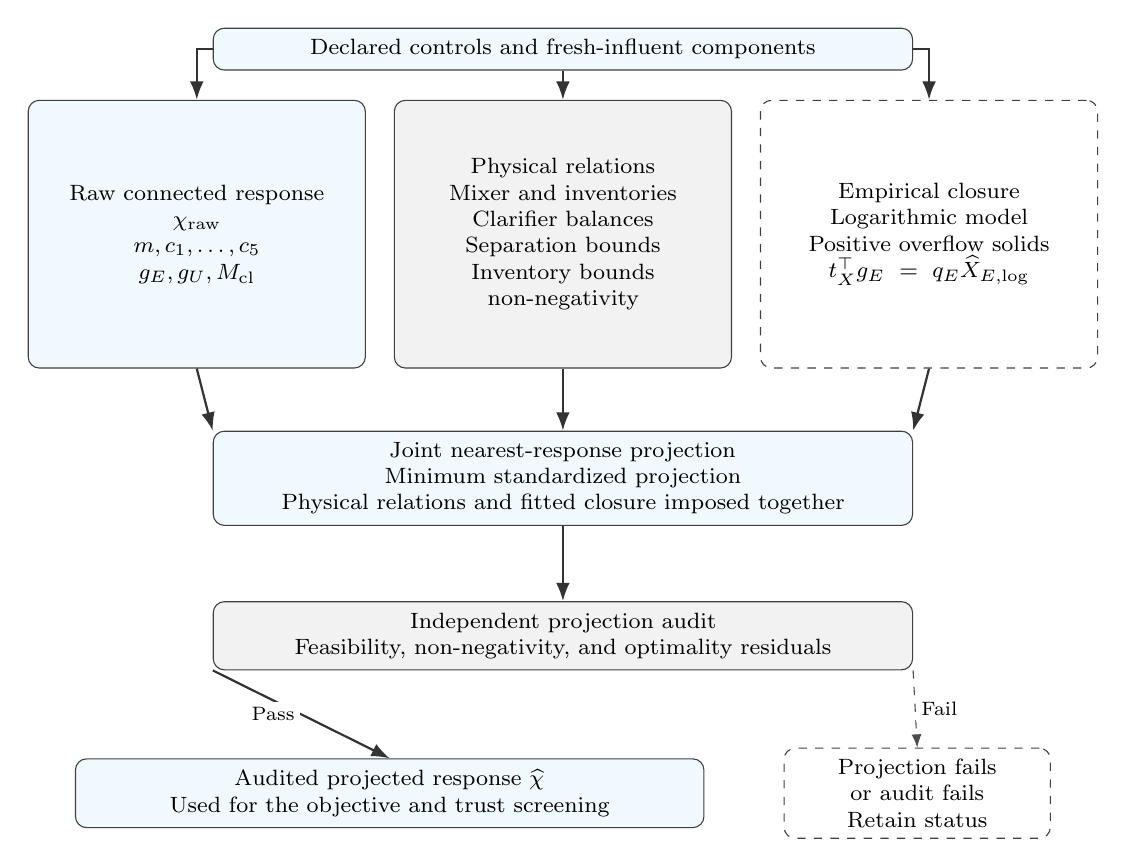
\begin{tikzpicture}[>=Latex,
block/.style={draw=black!75,rounded corners,fill=cyan!6,align=center,font=\footnotesize,inner sep=4pt},
physical/.style={block,fill=black!5},
empirical/.style={block,dashed,fill=white},
flow/.style={->,thick,draw=black!80},
failflow/.style={->,dashed,draw=black!70},
lab/.style={font=\scriptsize,fill=white,inner sep=2pt}]
\node[block,text width=8.6cm] (inputs) at (0,0) {Declared controls and fresh-influent components};
\node[block,text width=4.0cm,minimum height=3.4cm] (raw) at (-4.65,-2.35)
{Raw connected response\\$\chi_{\rm raw}$\\$m,c_1,\ldots,c_5$\\$g_E,g_U,M_{\rm cl}$};
\node[physical,text width=4.0cm,minimum height=3.4cm] (phys) at (0,-2.35)
{Physical relations\\Mixer and inventories\\Clarifier balances\\Separation bounds\\Inventory bounds\\non-negativity};
\node[empirical,text width=4.0cm,minimum height=3.4cm] (closure) at (4.65,-2.35)
{Empirical closure\\Logarithmic model\\Positive overflow solids\\$t_X^\top g_E=q_E\widehat X_{E,\log}$};
\node[block,text width=8.6cm] (projection) at (0,-5.45)
{Joint nearest-response projection\\Minimum standardized projection\\Physical relations and fitted closure imposed together};
\node[physical,text width=8.6cm] (audit) at (0,-7.45)
{Independent projection audit\\Feasibility, non-negativity, and optimality residuals};
\node[block,text width=7.7cm] (output) at (-2.2,-9.45)
{Audited projected response $\widehat\chi$\\Used for the objective and trust screening};
\node[empirical,text width=3.1cm] (failure) at (4.5,-9.45)
{Projection fails\\or audit fails\\Retain status};
\draw[flow] (inputs.south)--(phys.north);
\draw[flow] (inputs.west)-|(raw.north);
\draw[flow] (inputs.east)-|(closure.north);
\draw[flow] (raw.south)--(projection.north west);
\draw[flow] (phys.south)--(projection.north);
\draw[flow] (closure.south)--(projection.north east);
\draw[flow] (projection)--(audit);
\draw[flow] (audit.south west)--(output.north) node[midway,left,lab] {Pass};
\draw[failflow] (audit.south east)--(failure.north) node[midway,right,lab] {Fail};
\end{tikzpicture}
\caption{Conceptual information flow in the connected projection. The dashed closure block denotes an empirically fitted relation rather than a physical identity. Projection corrects all response blocks jointly. The audit checks the imposed relations at their numerical tolerances.}
\label{fig:plant_projection_architecture}
\end{figure}

The returned response is therefore the nearest admissible state under the stated response scales and constraint set. Both the physical rows and the empirical endpoint determine that set.

\subsubsection{Geometry of simultaneous physical enforcement}

Figure~\ref{fig:plant_projection_geometry} gives a geometric interpretation of Equation~\eqref{eq:plant_joint_projection}. Define the scaled response coordinates $\eta=D_\chi^{-1}\chi$ and the corresponding raw point $\eta_{\rm raw}=D_\chi^{-1}\chi_{\rm raw}$. These coordinates describe the response itself, whereas $u=\eta-\eta_{\rm raw}$ is the standardized displacement used above. Consequently, minimizing $\tfrac12u^\top u$ selects the point in the complete feasible set nearest to the raw response in this scaled geometry. Positive diagonal scaling retains the meaning of non-negativity while expressing concentrations, component flows and inventory in comparable scale units.

The analytical illustration uses the equality $\eta_1+\eta_2=1$, non-negativity $\eta_1,\eta_2\ge0$, and an additional inequality $\eta_1\ge0.20$. The equality defines a line. Non-negativity reduces it to the segment between $(0,1)$ and $(1,0)$, and the additional inequality restricts it further to the green segment between $(0.20,0.80)$ and $(1,0)$. The last inequality stands in for a separator or inventory restriction. Its numerical value is chosen only to make the geometry visible; it is not a case-study operating limit or a new plant-model assumption.

\begin{figure}[htbp]
\centering
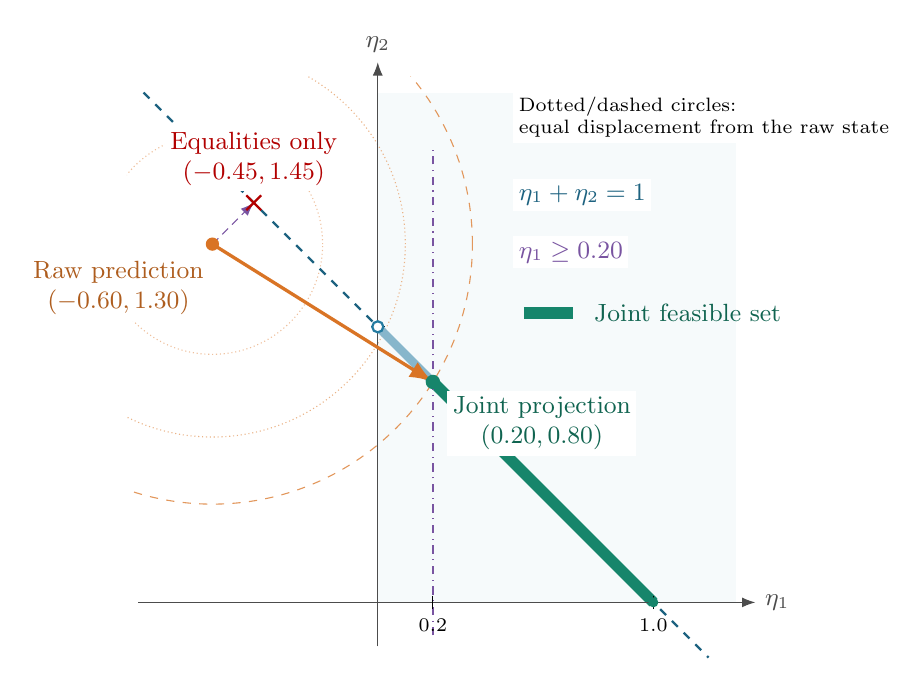
\begin{tikzpicture}[>=Latex,x=3.5cm,y=3.5cm,font=\small,
annotation/.style={fill=white,inner sep=2pt,align=center,font=\small}]
\fill[plantblue!4] (0,0) rectangle (1.30,1.85);
\begin{scope}
\clip (-.91,-.22) rectangle (1.31,1.91);
\draw[plantorange!45,densely dotted] (-.60,1.30) circle (.40);
\draw[plantorange!55,densely dotted] (-.60,1.30) circle (.70);
\draw[plantorange!75,dashed] (-.60,1.30) circle (.9433981);
\draw[plantblue!80!black,dashed,thick] (-.85,1.85)--(1.20,-.20);
\end{scope}
\draw[plantblue!55,line width=3pt] (0,1)--(1,0);
\draw[plantteal,line width=4pt] (.20,.80)--(1,0);
\draw[plantpurple,dash dot,thick] (.20,-.12)--(.20,1.65);
\draw[->,black!70] (-.87,0)--(1.37,0) node[right] {$\eta_1$};
\draw[->,black!70] (0,-.16)--(0,1.96) node[above] {$\eta_2$};
\foreach \tick in {0.2,1.0}{\draw (\tick,.025)--(\tick,-.025) node[below,font=\scriptsize] {$\tick$};}
\draw (.025,1)--(-.025,1);
\draw[plantorange,->,line width=1.2pt] (-.60,1.30)--(.20,.80);
\draw[plantpurple,->,densely dashed] (-.60,1.30)--(-.45,1.45);
\fill[plantorange] (-.60,1.30) circle (2.4pt);
\node[annotation,anchor=north east,text=plantorange!80!black] at (-.61,1.26) {Raw prediction\\$(-0.60,1.30)$};
\draw[red!70!black,thick] (-.477,1.423)--(-.423,1.477);
\draw[red!70!black,thick] (-.477,1.477)--(-.423,1.423);
\node[annotation,anchor=south,text=red!70!black] at (-.45,1.49) {Equalities only\\$(-0.45,1.45)$};
\draw[plantblue,fill=white,thick] (0,1) circle (2.0pt);
\fill[plantteal] (.20,.80) circle (2.6pt);
\node[annotation,anchor=north west,text=plantteal!75!black] at (.25,.77) {Joint projection\\$(0.20,0.80)$};
\fill[plantteal] (1,0) circle (1.8pt);
\node[annotation,anchor=west,text=plantblue!80!black] at (.49,1.48) {$\eta_1+\eta_2=1$};
\node[annotation,anchor=west,text=plantpurple] at (.49,1.27) {$\eta_1\ge0.20$};
\draw[plantteal,line width=4pt] (.53,1.05)--(.71,1.05);
\node[font=\small,anchor=west,text=plantteal!75!black] at (.75,1.05) {Joint feasible set};
\node[annotation,anchor=west,font=\scriptsize,align=left] at (.49,1.76) {Dotted/dashed circles:\\equal displacement from the raw state};
\end{tikzpicture}
\caption{Analytical illustration of joint plant-response projection in two scaled coordinates. The equality line, non-negativity and an additional inequality intersect to form the green feasible segment. The orange arrow gives the shortest admissible correction from the raw point, while the red cross shows an equality-only projection that remains negative. Circles denote equal standardized displacement from the raw point. The illustration explains the projection criterion and is not a simulated plant result.}
\label{fig:plant_projection_geometry}
\end{figure}

For the raw point $(-0.60,1.30)$, the nearest point on the equality line alone is $(-0.45,1.45)$. Its first coordinate is negative, so conservation alone does not make it admissible. The point $(0,1)$ satisfies the equality and non-negativity but still violates the additional inequality. The complete projection is instead $(0.20,0.80)$, where the smallest displacement circle that reaches the feasible segment meets its active boundary. Clipping the negative raw coordinate would give $(0,1.30)$ and violate the equality. A sequence of separate corrections therefore cannot be assumed to retain every previously satisfied relation.

In the connected plant, the same criterion acts on all mixer, reactor, outlet-flow and inventory coordinates together. A correction to one stream can require compensating changes at another location, and the fixed response scales determine the cost assigned to those movements. The diagram makes this simultaneous enforcement visible, but it does not prove agreement with the nonlinear kinetic or settling equations, nor does it establish predictive improvement relative to a reference outside the complete constraint set. The following weighted two-component example complements this geometric explanation by checking feasibility, multiplier signs, stationarity and complementarity explicitly.

\subsubsection{An independently auditable optimality certificate}

A simple two-component example illustrates how the projection can be checked independently. Let the raw prediction be $(-2,9)$, the coordinate scales be $(1,2)$, and the conserved total be 10. In physical coordinates,
\begin{equation}
\equationname{Illustrative weighted projection with mass conservation and non-negativity}
\min_{c_1,c_2}\ \frac12(c_1+2)^2+\frac18(c_2-9)^2,
\qquad c_1+c_2=10,\quad c_1\ge0,\quad c_2\ge0.
\end{equation}
The coefficient $1/8$ equals $1/(2\times2^2)$. A one-unit physical change in the second component is therefore less costly than the same change in the first because its scale is larger.

Ignoring non-negativity initially and introducing an equality multiplier $\lambda$ gives
\begin{align}
\equationname{Illustrative projection stationarity for the first component}
c_1+2+\lambda&=0,\\
\equationname{Illustrative projection stationarity for the second component}
\tfrac14(c_2-9)+\lambda&=0,\\
\equationname{Illustrative projection equality for the component total}
c_1+c_2&=10.
\end{align}
The first two equations imply $c_1=-2-\lambda$ and $c_2=9-4\lambda$. Substitution into the conserved-total equation gives $\lambda=-0.6$ and $(c_1,c_2)=(-1.4,11.4)$. Mass conservation alone therefore leaves the first component negative.

Imposing the active boundary $c_1=0$ forces $c_2=10$. Let $\mu_1,\mu_2\ge0$ be multipliers for $-c_1\le0$ and $-c_2\le0$. Because $c_2>0$, its inequality is inactive and $\mu_2=0$. Stationarity for component 2 gives $\lambda=-0.25$, and stationarity for component 1 gives $2-0.25-\mu_1=0$, so $\mu_1=1.75$. Both inequality multipliers are non-negative and both complementarity products vanish. These conditions certify the boundary solution instead of merely showing that it is feasible.

In standardized coordinates, $u=(2,0.5)^\top$, and the same problem becomes
\begin{equation}
\equationname{Standardized matrices of the illustrative two-component projection}
E=\begin{bmatrix}1&2\end{bmatrix},\quad e=3,\quad
G_u=\begin{bmatrix}-1&0\\0&-2\end{bmatrix},\quad
g=\begin{bmatrix}-2\\9\end{bmatrix}.
\end{equation}
The equality is $u_1+2u_2=3$, while the inequality rows are the physical non-negativity requirements after substitution. This form generalizes directly to the larger plant projection.

At fixed inputs, write the standardized problem as
\begin{equation}
\equationname{Standardized quadratic projection with equalities and inequalities}
\min_u\tfrac12u^\top u,\qquad Eu=e,\qquad G_uu\le g.
\label{eq:plant_standard_projection}
\end{equation}
Let $\lambda^=$ denote unrestricted equality multipliers and $\lambda^\le\ge0$ the inequality multipliers. Optimality requires primal feasibility, dual feasibility, stationarity, and complementarity,
\begin{align}
\equationname{Stationarity condition for the plant quadratic projection}
u+E^\top\lambda^=+G_u^\top\lambda^\le&=0,\\
\equationname{Complementarity condition for the projection inequality multipliers}
\lambda^\le_j(g_j-(G_uu)_j)&=0\quad\text{for every }j.
\label{eq:plant_projection_optimality}
\end{align}

The dual value follows by collecting the linear terms in the Lagrangian. Define $v=E^\top\lambda^=+G_u^\top\lambda^\le$. Completing the square gives
\begin{align}
\equationname{Completed-square expansion of the projection Lagrangian}
\tfrac12u^\top u+v^\top u-e^\top\lambda^=-g^\top\lambda^\le
&=\tfrac12\|u+v\|_2^2-\tfrac12\|v\|_2^2\\
\equationname{Target terms in the completed-square projection Lagrangian}
&\quad-e^\top\lambda^=-g^\top\lambda^\le.
\end{align}
The first term is minimized at $u=-v$, giving
\begin{equation}
\equationname{Dual objective of the standardized quadratic projection}
d(\lambda^=,\lambda^\le)=
-\tfrac12\|E^\top\lambda^=+G_u^\top\lambda^\le\|_2^2
-e^\top\lambda^=-g^\top\lambda^\le.
\end{equation}
For primal- and dual-feasible quantities, the resulting gap is
\begin{equation}
\equationname{Primal-dual gap and its non-negative decomposition}
\Gamma=\tfrac12\|u+E^\top\lambda^=+G_u^\top\lambda^\le\|_2^2
+(\lambda^\le)^\top(g-G_uu)\ge0.
\label{eq:plant_projection_gap}
\end{equation}
The gap vanishes exactly when stationarity and complementarity hold. This provides a mathematical certificate of the unique projection \citep{Boyd2004}. Numerical acceptance still checks each residual separately because a small aggregate gap does not replace explicit equality or non-negativity checks.

The two-component example permits direct verification of every certificate quantity. With $\lambda^{=}=-0.25$ and $\lambda^\le=(1.75,0)^\top$,
\begin{align}
\equationname{Illustrative cancellation of the stationarity residual}
E^\top\lambda^=+G_u^\top\lambda^\le&=(-2,-0.5)^\top=-u,\\
\equationname{Illustrative inequality slack vector}
g-G_uu&=(0,10)^\top,\\
\equationname{Illustrative value of the primal projection objective}
\tfrac12u^\top u&=\tfrac12(4+0.25)=2.125,\\
\equationname{Illustrative value of the dual projection objective}
d&=-2.125-3(-0.25)-[-2(1.75)]=2.125.
\end{align}
The primal and dual values agree. The stationarity residual is zero coordinate by coordinate, and the complementarity sum is $1.75(0)+0(10)=0$. A multiplier with the wrong sign would fail dual feasibility even if another residual were small.

Every distinct trial therefore receives an independently initialized projection solve. An operator-splitting quadratic solver of the type studied by \citet{Stellato2020} supplies the numerical candidate, while the audit reconstructs multipliers independently through bounded-variable least squares. Numerical retries may alter solver settings, but they do not alter the mathematical projection problem.

\subsubsection{Error bounds in the projection metric}

Let $\mathcal C$ denote the fixed-input feasible set and define the weighted norm
$\|v\|_{D_\chi^{-1}}=\|D_\chi^{-1}v\|_2$. Its scalar form is
\begin{equation}
\equationname{Weighted response norm from coordinate scales}
\|v\|_{D_\chi^{-1}}^2=\sum_{k=1}^{n_\chi}\frac{v_k^2}{s_k^2}.
\end{equation}
The geometric effect of projection can be derived most clearly in standardized coordinates. Write $a_k=\chi_{{\rm raw},k}/s_k$, $q_k=\widehat\chi_k/s_k$, and $t_k=\chi_{{\rm ref},k}/s_k$. The transformed feasible set remains convex because the scaling is an invertible linear transformation.

For any feasible comparison point $z$, the segment $q+\tau(z-q)$ remains feasible for $0\le\tau\le1$. Because $q$ minimizes distance from $a$, the projection objective cannot decrease along that segment. Its directional derivative at zero therefore satisfies
\begin{equation}
\equationname{Variational inequality characterizing a Euclidean projection}
\sum_k(q_k-a_k)(z_k-q_k)\ge0.
\end{equation}
If the reference itself is feasible, choose $z=t$. Reversing both signs gives $\sum_k(a_k-q_k)(q_k-t_k)\ge0$. For each coordinate,
\begin{align}
\equationname{Coordinatewise squared-error decomposition}
(a_k-t_k)^2&=(a_k-q_k)^2+(q_k-t_k)^2\\
\equationname{Cross term in the coordinatewise squared-error decomposition}
&\quad+2(a_k-q_k)(q_k-t_k).
\end{align}
Summing these identities gives
\begin{equation}
\equationname{Squared-error bound for a feasible reference}
\sum_k(q_k-t_k)^2\le\sum_k(a_k-t_k)^2-\sum_k(a_k-q_k)^2.
\end{equation}
The final sum is exactly the squared standardized projection distance. Returning to physical coordinates, if $\chi_{\rm ref}\in\mathcal C$,
\begin{equation}
\equationname{Weighted error reduction bound when the reference is projection-feasible}
\|\widehat\chi-\chi_{\rm ref}\|_{D_\chi^{-1}}^2
\le\|\chi_{\rm raw}-\chi_{\rm ref}\|_{D_\chi^{-1}}^2
-\|\widehat u\|_2^2.
\label{eq:plant_projection_error_exact}
\end{equation}
Projection therefore cannot increase aggregate squared error in this particular weighted metric to an exactly feasible reference. This result does not imply improvement in every component, every physical-unit score, or every operating objective, which are evaluated separately.

The earlier two-component problem illustrates this distinction. Let the feasible reference be $(3,7)$. Raw squared weighted error is $(-2-3)^2+(9-7)^2/4=26$, projected squared error is $(0-3)^2+(10-7)^2/4=11.25$, and projection-size squared is $2^2+0.5^2=4.25$. The bound gives $11.25\le26-4.25=21.75$. Yet the second component's absolute error increases from 2 to 3. Aggregate weighted improvement therefore does not require every component error to decrease.

The fitted overflow equality generally differs from the mechanistic endpoint, so the mechanistic reference need not lie in $\mathcal C$. Define its distance from the complete projection set by
\begin{equation}
\equationname{Distance from the reference state to the projection set}
\delta_{\rm feas}=\|P_{\mathcal C}(\chi_{\rm ref})-\chi_{\rm ref}\|_{D_\chi^{-1}}.
\end{equation}
Let $p$ denote the closest feasible point to $t$ in standardized coordinates. Applying the previous segment argument to $z=p$ gives
\begin{align}
\equationname{Cross-term decomposition using a projected reference}
\sum_k(a_k-q_k)(q_k-t_k)
&=\sum_k(a_k-q_k)(q_k-p_k)\\
\equationname{Reference-infeasibility term in the cross-term decomposition}
&\quad+\sum_k(a_k-q_k)(p_k-t_k).
\end{align}
The first term is non-negative. By Cauchy--Schwarz, the magnitude of the second is bounded by
\begin{equation}
\equationname{Product of projection displacement and reference infeasibility}
\left[\sum_k(a_k-q_k)^2\right]^{1/2}
\left[\sum_k(p_k-t_k)^2\right]^{1/2}
=r_{\rm corr}\delta_{\rm feas}.
\end{equation}
Here $r_{\rm corr}=\|\chi_{\rm raw}-P_{\mathcal C}(\chi_{\rm raw})\|_{D_\chi^{-1}}$. Expanding the squared error and applying this bound yields
\begin{align}
\equationname{Squared-error bound including reference infeasibility}
\|P_{\mathcal C}(\chi_{\rm raw})-\chi_{\rm ref}\|_{D_\chi^{-1}}^2
&\le\|\chi_{\rm raw}-\chi_{\rm ref}\|_{D_\chi^{-1}}^2
-r_{\rm corr}^2+2r_{\rm corr}\delta_{\rm feas}\\
\equationname{Upper error bound using squared reference infeasibility}
&\le\|\chi_{\rm raw}-\chi_{\rm ref}\|_{D_\chi^{-1}}^2+\delta_{\rm feas}^2.
\end{align}
Taking square roots gives the more interpretable bound
\begin{equation}
\equationname{Distance bound when the reference is not projection-feasible}
\|P_{\mathcal C}(\chi_{\rm raw})-\chi_{\rm ref}\|_{D_\chi^{-1}}
\le\|\chi_{\rm raw}-\chi_{\rm ref}\|_{D_\chi^{-1}}+\delta_{\rm feas}.
\label{eq:plant_projection_error_general}
\end{equation}
The distance term includes any mismatch between the mechanistic reference and the full projection set, including the empirical overflow equality. The weighted-projection discussion of \citet{SturmSilva2024} similarly separates mass conservation from predictive improvement. Independent original-model evaluation then checks the biological kinetics, nonlinear settling behavior, and local dynamic stability that projection does not enforce.

A hypothetical example shows why the empirical closure matters. Let the conserved total remain 10, but additionally require the first component to equal a fitted value of 4. The feasible set then contains only $(4,6)$. Suppose both the mechanistic reference and raw prediction are $(2,8)$ with scales $(1,2)$. The raw error is zero, but projection introduces weighted error $\sqrt{(4-2)^2+(6-8)^2/4}=\sqrt5$. The reference distance to the projection set is also $\sqrt5$, so the general bound is attained exactly. Treating only the physical identities as the feasible set would have incorrectly suggested the stronger exact-feasibility guarantee.

\subsubsection{Control-dependent sensitivities}

If the projection matrices were fixed and only the right-hand side depended affinely on parameters, the solution of a parametric quadratic program could be piecewise affine \citep{Tondel2003}. In the present formulation, however, both matrix coefficients and targets vary with the controls. Hydraulic ratios, inverse flow factors, the statistical feature vector, and the exponential overflow endpoint all depend on $\vartheta$. The projected plant response is therefore generally piecewise smooth where regularity conditions hold, with active-set changes defining boundaries between smooth regions.

A scalar example illustrates why derivatives of the constraint coefficients must be retained. Consider
\begin{equation}
\equationname{Scalar equality-constrained projection with a varying parameter}
\min_u\tfrac12u^2,\qquad b(\theta)u=e(\theta),
\end{equation}
with $b(\theta)\ne0$. Stationarity and feasibility are $u+b\lambda=0$ and $bu=e$, or
\begin{equation}
\equationname{Optimality system for the scalar parametric projection}
\begin{bmatrix}1&b\\b&0\end{bmatrix}
\begin{bmatrix}u\\\lambda\end{bmatrix}
=\begin{bmatrix}0\\e\end{bmatrix}.
\end{equation}
Differentiating both equations gives $u'+b'\lambda+b\lambda'=0$ and $b'u+bu'=e'$. Rearrangement yields
\begin{equation}
\equationname{Derivative system for the scalar parametric projection}
\begin{bmatrix}1&b\\b&0\end{bmatrix}
\begin{bmatrix}u'\\\lambda'\end{bmatrix}
=\begin{bmatrix}-b'\lambda\\e'-b'u\end{bmatrix}.
\end{equation}
The optimality matrix remains unchanged, while the right-hand side contains derivatives of both the coefficient and the target.

For $b=1+\theta$ and $e=\theta$, the solution is $u=\theta/(1+\theta)$ and $\lambda=-\theta/(1+\theta)^2$. At $\theta=1$, $u=0.5$ and $\lambda=-0.25$, giving
\begin{equation}
\equationname{Numerical example of the parametric projection derivative}
\begin{bmatrix}1&2\\2&0\end{bmatrix}
\begin{bmatrix}u'\\\lambda'\end{bmatrix}
=\begin{bmatrix}0.25\\0.5\end{bmatrix}.
\end{equation}
The second row gives $u'=0.25$, and the first gives $\lambda'=0$. Direct differentiation of $u=\theta/(1+\theta)$ gives the same result. Omitting $b'$ would instead differentiate a different optimization problem in which the constraint coefficient was incorrectly treated as constant.

For a stable active set, stack all equality rows and active inequality rows into $B(\vartheta)$, with corresponding right-hand side $b_a(\vartheta)$. The stationary system is
\begin{equation}
\equationname{Linear system for a fixed active set of projection constraints}
\begin{bmatrix}I&B^\top\\B&0\end{bmatrix}
\begin{bmatrix}u\\\lambda_a\end{bmatrix}
=\begin{bmatrix}0\\b_a\end{bmatrix}.
\label{eq:plant_active_system}
\end{equation}
Applying the product rule to $u+B^\top\lambda_a=0$ and $Bu=b_a$ gives
\begin{align}
\equationname{Differentiated stationarity for a control-dependent active set}
\partial_j u+B^\top\partial_j\lambda_a&=-(\partial_jB)^\top\lambda_a,\\
\equationname{Differentiated feasibility for a control-dependent active set}
B\partial_j u&=\partial_jb_a-(\partial_jB)u.
\end{align}
These equations combine into
\begin{equation}
\equationname{Joint sensitivity system for a control-dependent active set}
\begin{bmatrix}I&B^\top\\B&0\end{bmatrix}
\begin{bmatrix}\partial_j u\\\partial_j\lambda_a\end{bmatrix}
=\begin{bmatrix}-(\partial_jB)^\top\lambda_a\\
\partial_jb_a-(\partial_jB)u\end{bmatrix}.
\label{eq:plant_active_sensitivity}
\end{equation}
Because $D_\chi$ is fixed after fitting, the physical-response derivative is $\partial_j\widehat\chi=\partial_j\chi_{\rm raw}+D_\chi\partial_j\widehat u$.

The fitted overflow endpoint contributes an additional control-dependent target. Differentiating the scalar log prediction gives $\partial_j(\widehat\beta^\top\phi)=\widehat\beta^\top\partial_j\phi$. Exponentiation then gives $\partial_j\widehat X_{E,\log}=\widehat X_{E,\log}\widehat\beta^\top\partial_j\phi$, and the flow-weighted endpoint has derivative
\begin{equation}
\equationname{Derivative of the control-dependent overflow-solids target}
\partial_j(q_E\widehat X_{E,\log})
=(\partial_jq_E)\widehat X_{E,\log}
+q_E\widehat X_{E,\log}\widehat\beta_{E,\gamma_E}^\top\partial_j\phi.
\end{equation}
Ignoring this term would again differentiate a different optimization problem.

These derivatives are used only when the active rows are independent, the stationary matrix is well conditioned, active inequality multipliers are strictly positive, and independent perturbation checks pass. Near degeneracy, different active-set descriptions can correspond to the same unique projected state. Uniqueness of the projection therefore does not guarantee a reliable classical derivative. A value-only outer method remains available when the derivative chain cannot be validated.

\subsection{Treatment priorities, resource measures, and operating safeguards}

\subsubsection{A common engineering objective}

The effluent-quality map in Table~\ref{tab:component_basis_composites} gives
\begin{equation}
\equationname{Effluent component-to-water-quality map}
z_E=I_{\rm comp}c_E=\operatorname{col}(\mathrm{COD},\mathrm{TN},\mathrm{TP},\mathrm{TSS}).
\end{equation}
Let the diagonal entries of $D_T$ be $T_{COD},T_{TN},T_{TP},T_{TSS}$. Dividing each effluent quantity by its own scale makes the four quality terms dimensionless. With non-negative quality weights $\varpi_Q$ satisfying $\mathbf1^\top\varpi_Q=1$, the weighted quality score is
\begin{equation}
\equationname{Scalar expansion of the weighted effluent-quality objective}
\begin{aligned}
j_Q={}&\varpi_{Q,COD}\frac{z_{E,COD}}{T_{COD}}
+\varpi_{Q,TN}\frac{z_{E,TN}}{T_{TN}}\\
&+\varpi_{Q,TP}\frac{z_{E,TP}}{T_{TP}}
+\varpi_{Q,TSS}\frac{z_{E,TSS}}{T_{TSS}}.
\end{aligned}
\end{equation}
Equivalently,
\begin{equation}
\equationname{Vector form of the weighted effluent-quality objective}
j_Q=\varpi_Q^\top D_T^{-1}z_E.
\label{eq:plant_quality_objective}
\end{equation}
The four reported totals summarize different treatment concerns, but they do not identify the individual biological transformations that produce them. TN may remain nearly constant while ammonium is converted to nitrite or nitrate, and TP may decrease across the clarifier because particulate phosphorus is separated rather than because a new clarifier reaction occurs. The nutrient-control guidance of \citet{USEPA2009} and the component-resolved framework of \citet{Zhang2026} therefore support examining species and solids flows alongside aggregate treatment metrics.

Resource terms are normalized according to their physical interpretation. A bounded setting is placed between zero and one by subtracting its lower bound and dividing by its allowed range. Thus $H=18$ h in the interval 6--36 h gives $(18-6)/(36-6)=0.4$. Aeration is treated differently because its resource proxy is the total transfer capacity $\sum_iV_i k_La_i$, which has units of m$^3$ d$^{-1}$. Wasted solids are proportional to $Q_0wX_U$, and normalization by $Q_0w^UX_U^{\rm ref}$ cancels $Q_0$. The resulting terms are
\begin{align}
\equationname{Normalized retention-time and aeration objective terms}
j_H&=\frac{H-H^L}{H^U-H^L},\qquad
j_A=\frac{\sum_{i\in\mathcal A}V_i k_La_i}{E_A^{\rm ref}},\\
\equationname{Normalized mixed-liquor and return-sludge recycle objective terms}
j_I&=\frac{r_I-r_I^L}{r_I^U-r_I^L},\qquad
j_R=\frac{r_R-r_R^L}{r_R^U-r_R^L},\\
\equationname{Normalized waste-solids objective term}
j_W&=\frac{wX_U}{w^UX_U^{\rm ref}}.
\label{eq:plant_resource_objective}
\end{align}
The set $\mathcal A$ contains the aerated reactors. The reference $E_A^{\rm ref}>0$ is fixed before optimization as the maximum transfer-capacity numerator over the declared operating box. Fixing this denominator prevents a larger selected volume from being canceled by a simultaneously changing reference.

The aeration term represents transfer capacity rather than actual oxygen transfer, which also depends on the dissolved-oxygen deficit in Equation~\eqref{eq:plant_reactor}. The energy-management model of \citet{Miederer2025} separates aeration from other energy demands, while \citet{Zhang2026} explicitly retains the oxygen-transfer driving force. The present objective terms should therefore be read as dimensionless engineering measures of capacity and resource use.

Let the six overall coefficients correspond to the quality, HRT, aeration, internal recycle, return sludge, and wasting terms. The scalar objective is
\begin{equation}
\equationname{Scalar expansion of the six-term engineering objective}
J=\varpi_1j_Q+\varpi_2j_H+\varpi_3j_A+\varpi_4j_I+\varpi_5j_R+\varpi_6j_W.
\end{equation}
Its compact form is
\begin{equation}
\equationname{Vector engineering objective and normalized priority weights}
J(\vartheta,\chi,\varpi)=\varpi^\top
\operatorname{col}(j_Q,j_H,j_A,j_I,j_R,j_W),\qquad
\varpi\ge0,\quad\mathbf1^\top\varpi=1.
\label{eq:plant_engineering_objective}
\end{equation}
The vector $\varpi$ determines the trade-off between quality, capacity, and resource use, while $\varpi_Q$ determines the relative importance of COD, TN, TP, and TSS within the quality term. These coefficients encode preferences; they are not percentages of the realized objective.

For equal-volume reactors,
\begin{equation}
\equationname{Aeration objective for the illustrative equal-volume reactor train}
j_A=\frac{H}{36\ \mathrm{h}}\frac{a_3+a_4+a_5}{3}.
\label{eq:plant_aeration_proxy_example}
\end{equation}
This expression follows from $V_i=Q_0H/(24n_r)$ and $k_La_i=47a_i$. If all three aeration controls are at one, reducing $H$ from 36 h to 12 h reduces $j_A$ from one to one-third. The aeration settings have not changed, but the total installed transfer capacity has changed with reactor volume. A comparison based only on the dimensionless aeration controls would miss this capacity effect.

The baseline priorities are
\begin{equation}
\equationname{Declared engineering and effluent-quality priority vectors}
\varpi=(0.50,0.15,0.20,0.05,0.05,0.05)^\top,\qquad
\varpi_Q=\tfrac14\mathbf1_4.
\label{eq:plant_objective_priorities}
\end{equation}
Quality receives the largest overall weight, while aeration receives the largest resource weight. The importance of oxygen supply and solids age to treatment and energy use is discussed by \citet{Leu2012}. The exact values remain case-study choices. A different set of weights would define a different decision problem and would require its own reported optimization results.

A hypothetical calculation illustrates how the six terms combine. Let the effluent values be $(40,5,1,4)$ mg L$^{-1}$ and the fixed quality scales be $(100,10,2,20)$ mg L$^{-1}$. With equal quality priorities, $j_Q=(0.4+0.5+0.5+0.2)/4=0.4$. Let $H=18$ h, $(a_3,a_4,a_5)=(0.8,0.6,0.4)$, $r_I=1$, $r_R=0.5$, $w=0.02$, and $X_U=6{,}000$ g m$^{-3}$.

The total biological volume is $Q_0H/24=7{,}500$ m$^3$, so each of the five equal tanks has volume 1{,}500 m$^3$. Aeration capacity is $1{,}500(47)(0.8+0.6+0.4)=126{,}900$ m$^3$ d$^{-1}$. Table~\ref{tab:plant_hypothetical_objective} lists the normalized values and weighted contributions. Their sum is 0.353.

\begin{table}[htbp]
\centering\small
\caption{Hypothetical calculation of dimensionless objective contributions.}
\label{tab:plant_hypothetical_objective}
\begin{tabular}{llll}
\toprule Term & Calculation & Value & Weighted value\\\midrule
$j_Q$ & $(0.4+0.5+0.5+0.2)/4$ & 0.4 & 0.200\\
$j_H$ & $(18-6)/(36-6)$ & 0.4 & 0.060\\
$j_A$ & $126{,}900/423{,}000$ & 0.3 & 0.060\\
$j_I$ & $(1-0)/(4-0)$ & 0.25 & 0.0125\\
$j_R$ & $(0.5-0.25)/(1.25-0.25)$ & 0.25 & 0.0125\\
$j_W$ & $(0.02)(6{,}000)/[(0.05)(15{,}000)]$ & 0.16 & 0.008\\
\bottomrule
\end{tabular}
\end{table}

The overall quality weight of 0.50 multiplies $j_Q$ only after its four internal quality weights have been applied. An internal quality weight of one-quarter is therefore not an overall objective weight of one-quarter. Likewise, an objective reference value is not necessarily a feasibility limit. In particular, $j_W$ may exceed one if its numerator exceeds the declared reference. Normalization changes scale; it does not impose a hard bound.

\subsubsection{Solids retention time and clarifier loading}

Solids retention time combines stored solids mass with the rate at which solids leave the external plant boundary. For two reactors, stored solids would be $V_1X_1+V_2X_2+M_{\rm cl}$ in grams. The corresponding loss rate would be $Q_EX_E+Q_0wX_U$ in grams per day. Their ratio therefore has units of days. The same accounting applies to the five-reactor case.

External solids leave only through the clarifier overflow and the waste-sludge stream,
\begin{equation}
\equationname{External solids loss through effluent and waste sludge}
\dot M_X=Q_0(q_EX_E+wX_U).
\label{eq:plant_external_solids_loss}
\end{equation}
Return sludge is internal and does not contribute to external solids loss. With $X_i=t_X^\top c_i$, the plant solids retention time is
\begin{equation}
\equationname{Plant solids retention time from inventory and external loss}
\theta_X=\frac{\sum_{i=1}^{n_r}V_iX_i+M_{\rm cl}}{\dot M_X},
\qquad\dot M_X\ge\epsilon_X>0.
\label{eq:plant_solids_age}
\end{equation}
The clarifier inventory is part of the numerator. Omitting it would underestimate the solids age for a given external loss rate. Similarly, the wasting ratio alone cannot determine $\theta_X$ because both the product $wX_U$ and the internal solids inventory matter \citep{Alex2008}.

For illustration, let $Q_0=10{,}000$ m$^3$ d$^{-1}$, $w=0.02$, $X_E=10$, and $X_U=6{,}000$ g m$^{-3}$. The two external loss terms are
\begin{align}
\equationname{Illustrative effluent solids-loss calculation}
Q_0q_EX_E&=10{,}000(0.98)(10)=98{,}000\ \mathrm{g\,d^{-1}},\\
\equationname{Illustrative waste-sludge solids-loss calculation}
Q_0wX_U&=10{,}000(0.02)(6{,}000)=1{,}200{,}000\ \mathrm{g\,d^{-1}}.
\end{align}
Their total is 1{,}298{,}000 g d$^{-1}$. If the biological reactors contain 22{,}500{,}000 g of solids and the clarifier stores 7{,}500{,}000 g, total inventory is 30{,}000{,}000 g. The corresponding illustrative solids retention time is $30{,}000{,}000/1{,}298{,}000=23.11$ d.

Clarifier surface loading and solids loading describe different physical burdens on the separator. Surface loading divides overflow volume rate by clarifier area, while solids loading divides the feed solids mass rate by area \citep{Henze2008}. Because solids are represented in grams, a factor of $10^{-3}$ converts to kilograms:
\begin{equation}
\equationname{Clarifier surface and solids loading measures}
\ell_{\rm surface}=\frac{Q_0q_E}{A_{\rm cl}},\qquad
\ell_{\rm solids}=\frac{10^{-3}Q_0q_CX_N}{A_{\rm cl}}.
\label{eq:plant_loading_measures}
\end{equation}
The resulting units are m d$^{-1}$ and kg m$^{-2}$ d$^{-1}$, respectively. These quantities, together with $\theta_X$, are descriptive in the baseline comparison rather than optimization constraints.

For the same hypothetical fresh flow, take $r_R=0.5$, so $q_C=1.5$, with $A_{\rm cl}=1{,}500$ m$^2$ and $X_N=3{,}000$ g m$^{-3}$. The surface loading is $9{,}800/1{,}500=6.53$ m d$^{-1}$. The clarifier-feed solids rate is $10{,}000(1.5)(3{,}000)=45{,}000{,}000$ g d$^{-1}$, or 45{,}000 kg d$^{-1}$, giving a solids loading of 30 kg m$^{-2}$ d$^{-1}$. Using underflow solids in place of clarifier-feed solids would define a different loading measure.

The common engineering safeguards are
\begin{equation}
\equationname{Underflow, feed-solids, and external-loss safeguards}
X_U\le X_U^{\max},\qquad X_N\ge X_F^{\min}>0,\qquad
\dot M_X\ge\epsilon_X>0.
\label{eq:plant_engineering_safeguards}
\end{equation}
The feed-solids floor keeps particulate outlet reconstruction defined, while the external-loss floor keeps solids retention time defined. The underflow limit represents the admitted thickening or solids-handling range. Their numerical values are plant-specific inputs fixed before search. An underflow limit should reflect accepted sludge-handling conditions \citep{Henze2008}, whereas the feed and loss floors should prevent undefined calculations without excluding physically relevant low-solids operation. These safeguards are separate from the fixed $X_U^{\rm ref}=15{,}000$ g m$^{-3}$ used only to normalize the wasting objective.

\subsubsection{Trust diagnostics for operating search}

The trust diagnostics restrict the operating search to specified levels of data support and model consistency. They do not replace mechanistic verification. Instead, they test whether a candidate lies within an empirically supported part of the surrogate response and whether the projected state remains close to the raw prediction and compatible with selected mechanistic relations. The fixed thresholds therefore define the region in which the surrogate is permitted to support candidate selection. This role is consistent with approximation-management approaches such as \citet{Alexandrov1998} and \citet{Hameed2026}.

The projection diagnostic measures the root-mean-square standardized correction. For the hypothetical two-component projection $u=(2,0.5)$, it is $\sqrt{(4+0.25)/2}=1.458$. Dividing by the square root of the response dimension makes the quantity interpretable as an average standardized movement rather than a total movement that grows automatically with the number of response coordinates.

Feature leverage measures input support in the fitted quadratic feature space. In a hypothetical intercept-plus-one-feature example with development features $(-\sqrt{3/2},0,\sqrt{3/2})$ and $\gamma=1$,
\begin{equation}
\equationname{Illustrative regularized feature Gram matrix}
\Phi^\top\Phi+3\gamma R_\phi=
\begin{bmatrix}3&0\\0&6\end{bmatrix}.
\end{equation}
Its inverse is $\operatorname{diag}(1/3,1/6)$. At query feature $(1,z)$, leverage is $1/3+z^2/6$: it equals $1/3$ at the center, $1/2$ at $z=1$, and $11/6$ at $z=3$. The maximum development leverage in this example is $7/12$. The calculation shows how joint feature support weakens as a query moves away from the fitted design, even when individual controls remain inside their coordinate bounds.

The particulate split diagnostic asks whether all particulate components follow the common recovery relation used by Equation~\eqref{eq:plant_outlet_reconstruction}. Suppose two particulate components have unit TSS weights and feed concentrations $(40,60)$, so $X_N=100$. An underflow component-flow vector $(20,30)$ has total flow 50 and yields numerators $100(20)-50(40)=0$ and $100(30)-50(60)=0$. Reallocating the same total underflow solids to $(25,25)$ preserves aggregate solids but gives numerators 500 and $-500$. With fixed split scales of 500, the standardized residuals are 1 and $-1$, producing an RMS diagnostic of one. Aggregate solids consistency therefore does not establish composition consistency.

The reactor diagnostic measures the residual of the full smooth kinetic equations at the projected state. In the hypothetical two-component reactor discussed earlier, the projected concentrations $(9,6)$ preserve the upstream total $(12,3)$. With $d=2$ and reaction rate 8, the component residuals are $2(12-9)-8=-2$ and $2(3-6)+8=2$. If each balance scale is 10, the standardized residuals are $(-0.2,0.2)$ and the RMS diagnostic is 0.2. The invariant is satisfied even though the kinetic equations are not. This example makes the distinction between physical conservation and mechanistic-equation agreement explicit.

The four diagnostics are
\begin{align}
\equationname{Root-mean-square standardized projection displacement diagnostic}
\kappa_{\rm corr}&=\frac{\|D_\chi^{-1}(\widehat\chi-\chi_{\rm raw})\|_2}{\sqrt{n_\chi}},\\
\equationname{Ridge feature-leverage diagnostic}
\kappa_{\rm lev}&=\phi^\top(\Phi^\top\Phi+n_{\rm dev}\gamma R_\phi)^{-1}\phi,\\
\equationname{Particulate split-consistency diagnostic}
\kappa_{\rm split}&=\left[\frac1{F_X}\sum_{f\in X}
\left\{\frac{X_Ng_{U,f}-(t_X^\top g_U)c_{n_r,f}}{d_{{\rm split},f}}\right\}^2\right]^{1/2},\\
\equationname{Scaled reactor-equation residual diagnostic}
\kappa_{\rm reac}&=\frac{\|D_{\rm bal}^{-1}f_{{\rm sm},\rm reactor}(\vartheta,\widehat\chi)\|_2}{\sqrt{n_rF}}.
\label{eq:plant_trust_diagnostics}
\end{align}
The first measures the size of the physical correction applied to the raw surrogate response. The second measures data support in the fitted feature space. The third tests compatibility with the common particulate-recovery assumption. The fourth checks the smooth reactor equations at the projected concentrations. Clarifier-layer equations are assessed separately through the layer-resolved mechanistic model.

Residual scaling is based on the sizes of the physical terms before cancellation. Suppose a balance row contains terms $(100,-100)$ in one development state and $(200,-200)$ in another. Its net residual is zero in both states, but the individual terms are large. Their mean squared magnitude is $(100^2+100^2+200^2+200^2)/4=25{,}000$, giving an RMS scale of 158.11. Scaling only the net balance would discard this information. For a row with $p$ physical terms $b_{ij}$ over $n_{\rm dev}$ development states,
\begin{equation}
\equationname{Term-based scale for an independently checked residual}
d_b=\max\left\{1,\left[\frac1{n_{\rm dev}p}
\sum_{i=1}^{n_{\rm dev}}\sum_{j=1}^{p}b_{ij}^2\right]^{1/2}\right\}.
\label{eq:plant_term_scales}
\end{equation}
The same rule defines inequality and split scales. The overflow-closure scale uses the mechanistic overflow flow and the out-of-fold fitted endpoint flow as its two terms. The floor of one is expressed in the numerical units of the row and is not a concentration floor.

Projection, split, and reactor thresholds are set at the nearest-rank 95th percentile of grouped out-of-fold development diagnostics. If the sorted values are $v_{(1)},\ldots,v_{(n_{\rm dev})}$, the threshold is $v_{(\lceil0.95n_{\rm dev}\rceil)}$. The leverage threshold is the maximum development leverage under the final fitted feature map. These values are fixed before optimization. A diagnostic whose empirical threshold is zero remains constrained to zero; the value one is used only as a numerical row-scale floor.

The surrogate decision problem is therefore
\begin{equation}
\equationname{Surrogate-assisted plant operating optimization problem}
\begin{aligned}
\min_{\vartheta}\quad&J(\vartheta,\widehat\chi(\vartheta,c_{\rm in}),\varpi),\\
\text{subject to}\quad&\vartheta\in\mathcal V,\\
&g_{\rm eng}(\vartheta,\widehat\chi)\le0,\\
&g_{\rm trust}(\vartheta,\chi_{\rm raw},\widehat\chi)\le0,\\
&\widehat\chi\text{ satisfies Equation~\eqref{eq:plant_joint_projection}}.
\end{aligned}
\label{eq:plant_surrogate_optimization}
\end{equation}
The lower projection problem is convex, but the upper operating problem remains generally nonconvex because the statistical response, the control-dependent constraints, and the engineering objective are nonlinear in the controls. This nested structure is consistent with the bilevel perspective described by \citet{Colson2007}. The trust-region analysis of \citet{Alexandrov1998} further motivates supplementing average prediction accuracy with local admission checks near candidate operating points.

\subsection{Bounded products and convex relaxation}

The plant formulation also contains products of bounded variables, which helps explain why process optimization remains nonlinear even when the statistical coefficients themselves appear linearly. Let $x_L\leq x\leq x_U$, $y_L\leq y\leq y_U$, and let $z$ represent the product $xy$. The four quantities
\[
(x-x_L)(y-y_L),\quad (x_U-x)(y_U-y),\quad
(x_U-x)(y-y_L),\quad (x-x_L)(y_U-y)
\]
are non-negative. Expanding them and replacing $xy$ by $z$ gives the McCormick inequalities \citep{McCormick1976}
\begin{equation}
\equationname{McCormick inequalities for a bounded bilinear product}
\begin{aligned}
z&\geq x_Ly+y_Lx-x_Ly_L,\\
z&\geq x_Uy+y_Ux-x_Uy_U,\\
z&\leq x_Uy+y_Lx-x_Uy_L,\\
z&\leq x_Ly+y_Ux-x_Ly_U.
\end{aligned}
\label{eq:teaching_mccormick_relaxation}
\end{equation}
These inequalities are linear in $x$, $y$, and $z$, and every exact product satisfying the stated bounds obeys them. Their intersection is nevertheless larger than the exact nonlinear surface $z=xy$.

For example, if $0\leq x,y\leq1$, the inequalities reduce to $z\geq0$, $z\geq x+y-1$, $z\leq x$, and $z\leq y$. At $x=y=0.5$, they allow any $0\leq z\leq0.5$, while the exact product is only $z=0.25$. An objective value obtained at another permitted value of $z$ may therefore be a relaxation artifact rather than an attainable physical response. Tighter variable bounds can tighten the relaxation, but they do not generally recover the exact product relation. Process-network optimization uses this distinction when constructing bounds and interpreting solutions \citep{RubioCastro2013,YangNetwork2014}.

This example clarifies how convex relaxation differs from the projection used in this chapter. A relaxation enlarges a nonlinear feasible set to obtain a tractable optimization bound. The physical projection instead takes a statistical prediction and finds a nearby response satisfying the declared mass-conservation, non-negativity, separator, and inventory relations. The fixed plant topology is retained throughout both the surrogate-assisted and direct mechanistic searches.

\subsection{A direct mechanistic comparator}

\subsubsection{The full-state constrained optimization problem}

The direct route retains both the operating controls and the full reduced mechanistic state. It reconstructs $\chi(\vartheta,c_{\rm in},y)$ from that state and evaluates the same engineering objective used by the surrogate route. The finite-volume clarifier equations contain a positive feed-solids denominator at solver iterates. To keep this calculation defined during infeasible trial steps, an auxiliary variable $\widetilde X_F\ge X_F^{\min}$ supplies the denominator while feasibility requires $\widetilde X_F=t_X^\top c_{n_r}$.

A one-reactor, two-component, three-layer example illustrates the distinction between the direct and reduced formulations. The full state is $(c_S,c_X,s_1,s_2,s_3)$, which has five coordinates rather than the nine coordinates of $\chi_{\rm toy}$. With a simple conversion rate $kc_S$, the reactor equations are
\begin{align}
\equationname{Illustrative direct reactor equation for the consumed component}
0&=d(m_S-c_S)-kc_S,\\
\equationname{Illustrative direct reactor equation for the produced component}
0&=d(m_X-c_X)+kc_S.
\end{align}
The three clarifier equations are the layer balances defined earlier. The direct problem therefore imposes all five mechanistic equations, whereas the reduced physical projection retains only the aggregate reactor invariant and clarifier relations. Its three-layer envelope has two scalar inequalities, $s_1-s_2\le0$ and $s_2-s_3\le0$. Four layers would require $(s_1-s_2,s_1-s_3,s_2-s_4,s_3-s_4)\le0$. This pattern extends to the ten-layer case.

The auxiliary denominator has a numerical rather than physical role. During an infeasible trial, feed solids can approach zero while nonzero layer concentrations are still being adjusted. Division by the actual feed concentration would then be undefined. The bounded auxiliary $\widetilde X_F$ keeps the residual calculation finite. Because feasibility also imposes $\widetilde X_F=X_N$, it cannot be used to accept a zero-feed state as physically valid.

Let $f_{\rm sm}$ collect the $n_rF$ smooth reactor equations and the $L$ smooth clarifier-layer equations. Define
\begin{equation}
\equationname{Interior-layer envelope residuals for direct optimization}
g_{\rm env}(y)=\operatorname{col}
(s_1\mathbf1_{L-2}-s_{2:L-1},\ s_{2:L-1}-s_L\mathbf1_{L-2}).
\end{equation}
The direct nonlinear program is
\begin{equation}
\equationname{Direct mechanistic plant operating optimization problem}
\begin{aligned}
\min_{\vartheta,y,\widetilde X_F}\quad&J(\vartheta,\chi(\vartheta,c_{\rm in},y,\widetilde X_F),\varpi),\\
\text{subject to}\quad&f_{\rm sm}(\vartheta,c_{\rm in},y,\widetilde X_F)=0,\\
&\widetilde X_F=t_X^\top c_{n_r},\quad\widetilde X_F\ge X_F^{\min},\\
&\vartheta\in\mathcal V,\quad y\ge0,\quad g_{\rm env}(y)\le0,\\
&g_{{\rm eng},\rm red}(\vartheta,\chi)\le0.
\end{aligned}
\label{eq:plant_direct_optimization}
\end{equation}
The reduced engineering vector omits the feed-solids row because the auxiliary equality and lower bound already impose it. The auxiliary therefore changes only the numerical path taken through infeasible iterates, not the physical state admitted at feasibility.

\subsubsection{Smooth switches and continuation}

The exact kinetic and settling equations contain minima, maxima, positive parts, possible zero denominators, and a receiver switch. These operations are physically meaningful but introduce nondifferentiabilities or singular behavior that can hinder derivative-based optimization. The chemical-process treatment of \citet{BuzziFerraris2013} provides the broader context for derivative quality and numerical conditioning.

The exact identities
\begin{equation}
\equationname{Exact maximum and minimum expressed through absolute values}
\max(a,b)=\frac{a+b+|a-b|}{2},\qquad
\min(a,b)=\frac{a+b-|a-b|}{2}
\end{equation}
show that the nondifferentiability enters through $|a-b|$. Replacing $|r|$ by $\sqrt{r^2+\delta^2}$ produces a smooth approximation whenever $\delta>0$. The positive part uses the same substitution in $(v+|v|)/2$, whereas a potentially singular quotient uses a different regularization. For width $\delta=\epsilon S$,
\begin{align}
\equationname{Smooth approximation of a maximum}
\max_\delta(a,b)&=\tfrac12\left[a+b+\sqrt{(a-b)^2+\delta^2}\right],\\
\equationname{Smooth approximation of a minimum}
\min_\delta(a,b)&=\tfrac12\left[a+b-\sqrt{(a-b)^2+\delta^2}\right],\\
\equationname{Smooth approximation of the positive-part function}
[v]_{+,\delta}&=\tfrac12\left[v+\sqrt{v^2+\delta^2}\right],\\
\equationname{Regularized smooth approximation of a quotient}
\left(\frac ab\right)_\delta&=\frac{ab}{b^2+\delta^2}.
\label{eq:plant_smooth_operations}
\end{align}
For negative $v$, the positive-part approximation is evaluated as $\delta^2/[2(\sqrt{v^2+\delta^2}-v)]$ to avoid catastrophic cancellation. These approximations alter the equations near their switches, so the final selected controls are always reevaluated with the original nonsmoothed model.

For $a=2$, $b=1$, and $\delta=0.1$, the smooth maximum is 2.00249 and the smooth minimum is 0.99751, compared with exact values 2 and 1. For $v=-0.2$, the smooth positive part is 0.01180 rather than zero. At $b=0$, the regularized quotient remains defined and equals zero. At $a=1$, $b=0.1$, and $\delta=0.1$, it equals 5 rather than the exact quotient 10. These differences explain why the continuation gradually reduces the smoothing width and why an exact-model evaluation remains necessary.

The stable positive-part expression follows by rationalization,
\begin{align}
\equationname{Rationalization of the smoothed positive-part expression}
\frac{v+\sqrt{v^2+\delta^2}}2
&=\frac{(v+\sqrt{v^2+\delta^2})(\sqrt{v^2+\delta^2}-v)}
{2(\sqrt{v^2+\delta^2}-v)}\\
\equationname{Cancellation-resistant form of the smoothed positive part}
&=\frac{\delta^2}{2(\sqrt{v^2+\delta^2}-v)}.
\end{align}
The numerator reduces to $\delta^2$, eliminating subtraction of nearly equal terms.

The receiver switch is smoothed over a finite band around $X_t$. Subtracting the lower band edge $X_t-h$ and dividing by the full width $2h$ maps the transition interval to $[0,1]$. For receiver concentration $s$, the switch is zero below $X_t-h$, one above $X_t+h$, and
\begin{equation}
\equationname{Quintic receiver switch and its transition coordinate}
6\zeta^5-15\zeta^4+10\zeta^3,\qquad
\zeta=\frac{s-X_t+h}{2h}
\label{eq:plant_receiver_switch}
\end{equation}
inside the band. The quintic matches values and first two derivatives at both endpoints, producing a smooth transition between gravitational-flux rules.

For $X_t=3{,}000$ and $h=10$ g m$^{-3}$, concentrations 2{,}990, 3{,}000, and 3{,}010 correspond to $\zeta=0,0.5,1$ and switch values 0, 0.5, and 1. At 2{,}995, the switch is 0.10352; at 3{,}005, it is 0.89648. If $J_1$ denotes unrestricted gravitational flux and $J_2$ the receiver-limited flux, the smoothed interface uses $(1-\sigma)J_1+\sigma J_2$. The transition therefore modifies the flux law itself rather than merely smoothing a reported concentration.

Each smoothing scale $S$ is the development-set root mean square of the corresponding argument with a floor of one. Reactor scales are pooled across stages and include total oxidized nitrogen, fermentable substrate plus acetate, the hydrolysis denominator, polyphosphate and stored-carbon denominators, and remaining storage capacity. Clarifier scales include $s-f_{\rm ns}X_N$ and gravitational solids flux. The velocity scale is 250 m d$^{-1}$. These scales remain fixed during continuation.

The direct route uses three continuation stages,
\begin{equation}
\equationname{Smoothing and receiver-width continuation sequence}
(\epsilon,h)=(10^{-6},10),\ (10^{-7},3),\ (10^{-8},1),
\label{eq:plant_continuation_sequence}
\end{equation}
with $h$ in g TSS m$^{-3}$. Each stage initializes from the preceding solution. The sequence progressively sharpens the approximations while preserving a usable starting point. The final smooth candidate is still treated as a search output rather than as the final physical reference.

\subsubsection{Jacobian structure and globalization}

The direct mechanistic problem also benefits from its structured Jacobian. Entry $J_{jk}$ is the derivative of residual $f_j$ with respect to state coordinate $y_k$ and therefore describes how one balance responds to a local change in one state variable. For a hypothetical two-reactor soluble conversion with rate $kc_{i,S}$, soluble pass-through in the recycle gives
\begin{equation}
\equationname{Illustrative recycle-dependent soluble mixer concentration}
m_S=\frac{c_{{\rm in},S}+(r_I+r_R)c_{2,S}}{q_P}.
\end{equation}
The soluble residuals are $f_{1,S}=d_1(m_S-c_{1,S})-kc_{1,S}$ and $f_{2,S}=d_2(c_{1,S}-c_{2,S})-kc_{2,S}$. Their Jacobian block is
\begin{equation}
\equationname{Illustrative two-stage reactor Jacobian with recycle coupling}
\frac{\partial(f_{1,S},f_{2,S})}{\partial(c_{1,S},c_{2,S})}
=\begin{bmatrix}
-(d_1+k)&d_1(r_I+r_R)/q_P\\
d_2&-(d_2+k)
\end{bmatrix}.
\end{equation}
The upper-right entry arises entirely from recycle: changing the final-reactor concentration changes the mixer and therefore changes the first-reactor residual. Ignoring this term would incorrectly treat the mixer as independent of the downstream state. With $d_1=d_2=2$, $k=1$, $r_I=1$, $r_R=0.5$, and $q_P=2.5$, the block is $\begin{bmatrix}-3&1.2\\2&-3\end{bmatrix}$.

Finite differences provide an independent check on such derivatives. Increasing $c_{1,S}$ by 0.01 g m$^{-3}$ changes $f_{1,S}$ by $-0.03$ g m$^{-3}$ d$^{-1}$, giving derivative $-3$. Increasing $c_{2,S}$ by the same amount changes $m_S$ by 0.006 and $f_{1,S}$ by 0.012, giving 1.2. For a nonlinear residual, the corresponding central difference is
\begin{equation}
\equationname{Central finite-difference approximation of a Jacobian entry}
J_{jk}\approx\frac{f_j(y+he_k)-f_j(y-he_k)}{2h}.
\end{equation}
Near a non-negative boundary, a symmetric perturbation may leave the admissible state region. A second-order forward difference is then used,
\begin{equation}
\equationname{Second-order forward finite-difference approximation of a Jacobian entry}
J_{jk}\approx\frac{-3f_j(y)+4f_j(y+he_k)-f_j(y+2he_k)}{2h}.
\end{equation}
The perturbation $h$ retains the physical units of $y_k$. Scaling coordinates keeps its relative size comparable across different component bases.

For three clarifier layers at fixed feed conditions, each interface involves only neighboring layers. The layer Jacobian therefore has the tridiagonal pattern
\begin{equation}
\equationname{Tridiagonal sparsity pattern of the clarifier-layer Jacobian}
J_{\rm layer}=\begin{bmatrix}\star&\star&0\\\star&\star&\star\\0&\star&\star\end{bmatrix},
\end{equation}
where $\star$ indicates a potentially nonzero entry. Feed solids and outlet reconstruction add couplings to reactor coordinates. The zeros are consequences of the declared dependency structure rather than approximations introduced for computational convenience.

The complete direct residual remains sparse. A reactor balance depends primarily on its own component vector and the preceding stage, with additional recycle dependence on final-reactor and underflow quantities. A clarifier layer depends on neighboring layer concentrations, feed solids, and hydraulic controls. Inventory and reporting maps are linear aggregations. These local dependencies produce a structured Jacobian rather than an arbitrary dense response map.

Scaling is applied before Jacobian conditioning or residual magnitudes are assessed. The component basis includes oxygen, COD, nitrogen, phosphorus, solids, and charge equivalents, so an unscaled norm could be dominated by a large solids balance while concealing a nutrient-balance defect. Analytic derivatives or differentiated smooth equations supply the optimization Jacobian, while independent finite differences remain available for derivative verification. Sparse linear algebra exploits the local reactor and layer structure without dropping recycle couplings.

The direct search uses the interior-point filter method studied by \citet{WachterBiegler2006}. Its line search balances progress in objective value and constraint violation. This globalization mechanism governs acceptance of local steps during the search. As with the surrogate route, numerical search progress remains distinct from the final physical and stationarity audits.

\section{Methodology}

\subsection{Case-study domain and fixed parameters}

\subsubsection{Topology and free controls}

The case study contains five equal-volume biological reactors and ten clarifier layers. Reactors 1 and 2 are unaerated, while reactors 3--5 have independent aeration controls. The free-control vector is
\begin{equation}
\equationname{Seven freely varied controls of the connected-plant case}
\vartheta=(H,a_3,a_4,a_5,r_I,r_R,w)^\top\in\mathbb R^7.
\label{eq:plant_case_controls}
\end{equation}
For all five stages, $h_i=H/5$. The unaerated controls are fixed at $a_1=a_2=0$, the aerated-stage transfer coefficients are $k_La_i=47a_i$ d$^{-1}$, and $\xi_i=0$. These choices define the present case study; they are not structural requirements of the connected formulation.

\begin{table}[htbp]
\centering\small
\caption{Plant geometry and operating domain.}
\label{tab:plant_operating_domain}
\begin{tabular}{p{0.47\linewidth}p{0.40\linewidth}}
\toprule
Quantity & Value or interval\\
\midrule
Fresh-influent flow $Q_0$ & 10{,}000 m$^3$ d$^{-1}$\\
Reactors $n_r$, layers $L$, feed layer $\ell_F$ & 5, 10, 5\\
Reactor volume fraction $f_i^V$ & $1/5$ for every stage\\
Clarifier area and total depth & 1{,}500 m$^2$ and 4.0 m\\
Clarifier total and individual layer volumes & 6{,}000 m$^3$ and 600 m$^3$\\
Nominal total HRT $H$ & 6--36 h\\
Each of $a_3,a_4,a_5$ & 0--1 independently\\
Mixed-liquor recycle $r_I$ & 0--4\\
Return-sludge ratio $r_R$ & 0.25--1.25\\
Waste-sludge ratio $w$ & 0.001--0.05\\
Aeration reference $E_A^{\rm ref}$ & 423{,}000 m$^3$ d$^{-1}$\\
Wasted-solids reference $X_U^{\rm ref}$ & 15{,}000 g TSS m$^{-3}$\\
\bottomrule
\end{tabular}
\end{table}

The equal-volume reactors provide a compact unaerated-to-aerated treatment train. Each clarifier layer has depth 0.4 m. The operating bounds preserve positive overflow and underflow flow ratios throughout the domain. Together with the 20 fresh-influent components, the seven free controls produce 27 statistical inputs, 406 quadratic features, and 161 reduced-response coordinates. The mechanistic state contains 110 coordinates. The connected projection contains 76 equality rows and 12 physical inequality rows; after response non-negativity is included, the total number of inequality rows is 173.

Changing the number of reactors or free controls changes the statistical input and response dimensions. Changing the clarifier-layer count changes the mechanistic state and inventory mapping but does not add coordinates to the aggregate surrogate response. In either case, the fitted models, physical constraints, and predictive validation would need to be re-established. The layer discretization affects the mechanistic targets and the admissible inventory bounds even though the surrogate stores only aggregate clarifier inventory.

\subsubsection{Fresh-influent intervals}

Table~\ref{tab:plant_influent_intervals} defines the independent fresh-influent intervals used in the connected-plant experiment. The nominal influent is the componentwise midpoint of these intervals. Concentration bases and the composite reporting weights follow Table~\ref{tab:component_basis_composites}. The plant alkalinity interval is 1.6--5.2 mol charge equivalents m$^{-3}$.

\begin{table}[htbp]
\centering\small
\caption{Independent fresh-influent intervals for the connected plant.}\label{tab:plant_influent_intervals}
\begin{tabular}{lrrl}
\toprule
Component & Lower & Upper & Constituent basis\\
\midrule
$S_O$ & 0 & 0.5 & oxygen\\
$S_F$ & 20 & 180 & COD\\
$S_A$ & 5 & 80 & COD\\
$S_{NH4}$ & 12 & 55 & nitrogen\\
$S_{NO2}$ & 0 & 3 & nitrogen\\
$S_{NO3}$ & 0 & 8 & nitrogen\\
$S_{N2}$ & 0 & 2 & nitrogen\\
$S_{PO4}$ & 2 & 18 & phosphorus\\
$S_I$ & 10 & 90 & COD\\
$S_{ALK}$ & 1.6 & 5.2 & charge equivalents\\
$X_I$ & 20 & 120 & COD\\
$X_S$ & 60 & 280 & COD\\
$X_H$ & 15 & 100 & COD\\
$X_{PAO}$ & 5 & 60 & COD\\
$X_{PP}$ & 2 & 20 & phosphorus\\
$X_{PHA}$ & 1 & 30 & COD\\
$X_{AOB}$ & 0.5 & 8 & COD\\
$X_{NOB}$ & 0.5 & 8 & COD\\
$X_{MeP}$ & 0 & 12 & solids\\
$X_{MeOH}$ & 0 & 12 & solids\\
\bottomrule
\end{tabular}
\end{table}

All concentration values are expressed as grams of the stated constituent per m$^3$, except alkalinity. Numerically, g m$^{-3}$ equals mg L$^{-1}$. Independent interval sampling distributes candidates throughout the declared experimental domain without imposing correlations among the input coordinates.

\subsubsection{Stoichiometric, kinetic, and settling parameters}

Tables~\ref{tab:plant_stoichiometric_constants}--\ref{tab:plant_settling_constants} list the fixed parameters used in the connected-plant case. These quantities define the mechanistic reference model and are not fitted from the surrogate data. Each concentration-based parameter follows the constituent basis of its associated component. Symbols grouped on one row share a common numerical value. The two nitrifier populations remain distinct through their different growth rates and oxygen half-saturation constants.

\begin{table}[htbp]
\centering\small
\caption{Fixed yields, constituent contents, and conversion factors.}\label{tab:plant_stoichiometric_constants}
\begin{tabular}{p{0.38\linewidth}p{0.13\linewidth}p{0.38\linewidth}}
\toprule Parameter & Value & Unit or interpretation\\\midrule
$Y_H,Y_{PAO}$ & 0.625 & g biomass COD per g substrate COD\\
$Y_{PHA}$ & 0.20 & g stored COD per g phosphorus\\
$Y_{PO4}$ & 0.40 & g phosphorus per g stored COD\\
$Y_{AOB}$ & 0.18 & g biomass COD per g nitrogen\\
$Y_{NOB}$ & 0.08 & g biomass COD per g nitrogen\\
$f_{SI}$ & 0 & soluble inert fraction\\
$f_{XI}$ & 0.10 & particulate inert fraction\\
$i_{N,SI}$ & 0.01 & g nitrogen per g COD\\
$i_{N,SF},i_{N,XS}$ & 0 & g nitrogen per g COD\\
$i_{N,XI}$ & 0.02 & g nitrogen per g COD\\
$i_{N,BM}$ & 0.07 & g nitrogen per g biomass COD\\
$i_{P,SI},i_{P,SF},i_{P,XS}$ & 0 & g phosphorus per g COD\\
$i_{P,XI}$ & 0.01 & g phosphorus per g COD\\
$i_{P,BM}$ & 0.02 & g phosphorus per g biomass COD\\
$i_{P,MeP}$ & $1/4.87$ & g phosphorus per g metal-phosphate solids\\
$\gamma_{OH}$ & 3.45 & g metal-hydroxide solids per g phosphorus\\
\bottomrule
\end{tabular}
\end{table}

\begin{table}[htbp]
\centering\small
\caption{Fixed hydrolysis and heterotrophic rate and saturation constants.}
\label{tab:plant_kinetic_constants}
\begin{tabular}{p{0.48\linewidth}p{0.10\linewidth}p{0.31\linewidth}}
\toprule Parameter & Value & Unit\\\midrule
$K_H$ & 3.0 & d$^{-1}$\\
$\eta_{{\rm hyd},NO3},\eta_{{\rm hyd},NO2}$ & 0.6 & dimensionless\\
$\eta_{{\rm hyd},fe}$ & 0.4 & dimensionless\\
$K_{O,\rm hyd},K_{O,H},K_{O,PAO}$ & 0.20 & g oxygen m$^{-3}$\\
$K_{NO3,\rm hyd},K_{NO2,\rm hyd},K_{NOx,\rm hyd}$ & 0.5 & g nitrogen m$^{-3}$\\
$K_X$ & 0.10 & g substrate COD per g biomass COD\\
$\mu_H$ & 6.0 & d$^{-1}$\\
$q_{fe}$ & 3.0 & d$^{-1}$\\
$b_H$ & 0.40 & d$^{-1}$\\
$\eta_{H,NO3},\eta_{H,NO2}$ & 0.9 & dimensionless\\
$K_F,K_{fe},K_A$ & 4.0 & g COD m$^{-3}$\\
$K_{NO3,H},K_{NO2,H},K_{NOx,H}$ & 0.5 & g nitrogen m$^{-3}$\\
$K_{NH4,H},K_{NH4,PAO},K_{NH4,NOB}$ & 0.05 & g nitrogen m$^{-3}$\\
$K_{PO4,H},K_{PO4,PAO},K_{PO4,\rm nit}$ & 0.01 & g phosphorus m$^{-3}$\\
$K_{ALK,H},K_{ALK,PAO}$ & 0.10 & mol equivalents m$^{-3}$\\
\bottomrule
\end{tabular}
\end{table}

\begin{table}[htbp]
\centering\small
\caption{Fixed storage, nitrifier, and chemical rate and saturation constants.}
\label{tab:plant_storage_nitrifier_constants}
\begin{tabular}{p{0.48\linewidth}p{0.10\linewidth}p{0.31\linewidth}}
\toprule Parameter & Value & Unit\\\midrule
$q_{PHA}$ & 5.0 & g stored COD per g biomass COD per d\\
$q_{PP}$ & 0.60 & g phosphorus per g biomass COD per d\\
$\mu_{PAO}$ & 0.56 & d$^{-1}$\\
$\eta_{PAO,NO3}$ & 0.07 & dimensionless\\
$\eta_{PAO,NO2}$ & 0.90 & dimensionless\\
$b_{PAO},b_{PP},b_{PHA},b_{AOB}$ & 0.20 & d$^{-1}$\\
$K_{NO3,PAO},K_{NO2,PAO},K_{NOx,PAO}$ & 0.5 & g nitrogen m$^{-3}$\\
$K_{PS}$ & 0.20 & g phosphorus m$^{-3}$\\
$K_{PP}$ & 0.01 & g phosphorus per g biomass COD\\
$K_{\max}$ & 0.34 & g phosphorus per g biomass COD\\
$K_{IPP}$ & 0.02 & g phosphorus per g biomass COD\\
$K_{PHA}$ & 0.01 & g stored COD per g biomass COD\\
$\mu_{AOB}$ & 1.81 & d$^{-1}$\\
$\mu_{NOB}$ & 1.52 & d$^{-1}$\\
$b_{NOB}$ & 0.17 & d$^{-1}$\\
$K_{O,AOB}$ & 0.74 & g oxygen m$^{-3}$\\
$K_{O,NOB}$ & 1.75 & g oxygen m$^{-3}$\\
$K_{NH4,AOB},K_{NO2,NOB}$ & 0.5 & g nitrogen m$^{-3}$\\
$K_{ALK,\rm nit},K_{ALK,PRE},K_{ALK,\rm chem}$ & 0.50 & mol equivalents m$^{-3}$\\
$k_{PRE}$ & 1.0 & m$^3$ per g solids per d\\
$k_{RED}$ & 0.60 & d$^{-1}$\\
\bottomrule
\end{tabular}
\end{table}

\begin{table}[htbp]
\centering\small
\caption{Fixed settling and oxygen-transfer parameters.}
\label{tab:plant_settling_constants}
\begin{tabular}{p{0.46\linewidth}p{0.39\linewidth}}
\toprule Quantity & Value\\\midrule
Maximum settling velocity $v_{\max}$ & 250 m d$^{-1}$\\
Theoretical settling velocity $v_0$ & 474 m d$^{-1}$\\
Hindered-settling coefficient $r_h$ & 0.000576 m$^3$ per g TSS\\
Low-concentration coefficient $r_p$ & 0.00286 m$^3$ per g TSS\\
Nonsettleable fraction $f_{\rm ns}$ & 0.00228\\
Receiver threshold $X_t$ & 3{,}000 g TSS m$^{-3}$\\
Oxygen saturation $S_O^*$ & 8.5 g oxygen m$^{-3}$\\
Maximum aerated-stage $k_La$ & 47 d$^{-1}$\\
\bottomrule
\end{tabular}
\end{table}

\subsection{Mechanistic sampling, fitting, and prediction assessment}

\subsubsection{Simulation groups and accepted cases}

The connected input domain contains seven operating controls and twenty fresh-influent components. Strength-one Latin-hypercube sampling is used to distribute candidates across this 27-dimensional space. Each coordinate receives one point in every marginal stratum. Independent random permutations prevent the same ordering from being shared across coordinates, while open-unit jitter places each sampled value strictly inside its selected stratum. The coverage rationale follows the sampling design of \citet{McKay1979}.

The study attempts 8{,}000 development candidates and 2{,}000 holdout candidates using separate seeded random streams. Rejected candidates remain part of the accounting and are not replaced. A two-start physical acceptance procedure determines which attempted cases become statistical states. Acceptance and rejection counts are reported separately for the development and holdout designs.

\begin{table}[htbp]
\centering\small
\caption{Randomization and fitting settings specified before assessment.}
\label{tab:plant_design_settings}
\begin{tabular}{p{0.54\linewidth}p{0.32\linewidth}}
\toprule Setting & Value\\\midrule
Development Latin-hypercube seed & 100042\\
Holdout Latin-hypercube seed & 100043\\
Influent-scenario Latin-hypercube seed & 314159\\
Grouped-fold permutation seed & 271828\\
Number of fitting folds & 5\\
Raw-response and logarithmic ridge grids & $\{10^{-8},10^{-7},\ldots,10^2\}$\\
Standard-deviation divisor & fitting-set size\\
Near-constant coordinate cutoff & $10^{-12}\max(1,\max_i|v_i|)$\\
Low-overflow group & at or below development 25th percentile\\
High-overflow group & at or above development 90th percentile\\
\bottomrule
\end{tabular}
\end{table}

A four-stratum example illustrates the Latin-hypercube mapping. Each unit-interval stratum has width $1/4$. Selecting stratum two with within-stratum fraction 0.6 gives $(2+0.6)/4=0.65$. If the physical coordinate spans 10 to 20, this maps to $10+0.65(20-10)=16.5$. Independent permutations of the remaining coordinates retain marginal coverage while avoiding a shared coordinate ordering.

The exact jitter rule uses the same idea at much finer resolution. Dividing an unsigned 64-bit random integer $U$ by $2^{11}$ and taking the floor gives an integer from zero to $2^{53}-1$. Adding 0.5 selects the midpoint of that fine stratum, and division by $2^{53}$ maps it to the open unit interval. Thus
\begin{equation}
\equationname{Conversion of a uniform integer to open-unit jitter}
\zeta_U=\frac{\lfloor U/2^{11}\rfloor+0.5}{2^{53}}\in(0,1).
\end{equation}
In exact arithmetic, the extreme values are $2^{-54}$ and $1-2^{-54}$. The procedure therefore excludes exact stratum boundaries, although endpoint checks remain necessary after finite-precision mapping to physical variables.

Each coordinate uses a descending Fisher--Yates permutation of its strata. Accepted mechanistic states retain their original candidate order before the grouped-fold permutation is applied. The fitting and prediction assessments therefore use only states that have already passed the mechanistic integration, balance, branch, and stability checks, while rejection counts preserve the outcomes of the attempted design.

\subsubsection{Two initial states and the nonsmoothed steady solve}

Mechanistic generation uses two deliberately different initial conditions. The first assigns $c_{\rm in}$ to every reactor and fresh-influent TSS to every clarifier layer. The second retains the fresh soluble concentrations but multiplies the particulate concentrations in reactors 1--5 by $(1.5,2,2.5,3,3.5)$. Its final-reactor TSS then sets the initial clarifier profile through
\begin{equation}
\equationname{Ten-layer initial solids-profile multipliers}
(0.002,0.005,0.01,0.03,0.10,0.50,1.25,2.25,3.25,4.00)
\label{eq:plant_initial_layer_multipliers}
\end{equation}
from the surface to the hopper. The two starts probe sensitivity to distinct biomass and storage states. Agreement between their converged physical states is part of the acceptance procedure.

A logarithmic transformation keeps integrated coordinates positive. For a positive native-coordinate value $y_f$, define $\eta_f=\log y_f$. Because $y_f=\exp(\eta_f)$,
\[
\begin{aligned}
y_f&=\exp(\eta_f),\\
\frac{\mathrm d y_f}{\mathrm dt}
&=\exp(\eta_f)\frac{\mathrm d\eta_f}{\mathrm dt}
=y_f\frac{\mathrm d\eta_f}{\mathrm dt}.
\end{aligned}
\]
The original balance requires $\mathrm d y_f/\mathrm dt=f_f(y)$, so
$\mathrm d\eta_f/\mathrm dt=f_f(y)/y_f$. The transformation therefore changes only the numerical coordinates, not the underlying physical balance.

For example, if a concentration is 2 native units and its balance rate is $-0.4$ native units per day, the transformed rate is $-0.2$ d$^{-1}$. A half-day illustrative Euler step in $\eta$ gives
\[
\eta_{new}=\log2+0.5(-0.2),\qquad
y_{new}=\exp(\eta_{new})=2\exp(-0.1)\approx1.8097.
\]
The actual integration uses the backward differentiation method with the numerical tolerances specified below; this arithmetic is only intended to show the effect of the positive-state transformation.

Before the logarithmic transformation, any initial coordinate below $10^{-8}$ is raised to $10^{-8}$ in its native physical unit. This safeguard applies only to initialization and is distinct from clipping a final solution or prediction.

The integration horizon depends on wasting because low wasting can lead to long solids residence times. It is defined as
\begin{equation}
\equationname{Waste-dependent horizon for dynamic relaxation}
T=\max\{400,50/\max(w,0.001)\}\ \mathrm{d}.
\label{eq:plant_integration_horizon}
\end{equation}
At $w=0.01$, this gives 5{,}000 d; at $w=0.20$, it gives the 400-d minimum; and at $w=0$, the internal floor gives 50{,}000 d. The values zero and 0.20 are used only to illustrate the branches of the rule and lie outside the admitted case-study wasting interval.

Dynamic relaxation uses the backward differentiation method for stiff systems \citep{CurtissHirschfelder1952}. The integration may stop before $T$ when the scaled residual falls below $10^{-9}$. Its purpose is to produce a physically informed initial state for the algebraic steady calculation, consistent with the continuation rationale of \citet{KelleyKeyes1998} and the activated-sludge procedure of \citet{Selerio2026}. A bounded least-squares polishing calculation is attempted only if the integrated endpoint fails the physical audit. Solver convergence and scientific acceptance are therefore kept separate.

\begin{table}[htbp]
\centering\small
\caption{Steady-state generation and physical acceptance settings.}\label{tab:plant_generation_settings}
\begin{tabular}{p{0.61\linewidth}p{0.25\linewidth}}
\toprule Setting & Value\\\midrule
Integration relative tolerance & $10^{-7}$\\
Transformed integration absolute tolerance & $10^{-9}$\\
Maximum integration step & $T/100$\\
Polishing evaluation limit & 5{,}000\\
Polishing step, function, and gradient tolerances & $10^{-9}$ each\\
Term-scaled balance tolerance & $10^{-6}$\\
State non-negativity tolerance & $10^{-10}$\\
Reaction-rate non-negativity tolerance & $10^{-12}$\\
Two-start scaled state agreement & $10^{-6}$\\
Rightmost reduced-state Jacobian eigenvalue & at most $-10^{-8}$ d$^{-1}$\\
Eigenvalue agreement between two step sizes & $10^{-6}$ d$^{-1}$\\
Matrix mass conservation and rank audit tolerance & $10^{-10}$\\
\bottomrule
\end{tabular}
\end{table}

The balance audit scales each residual relative to the physical terms that form it. Suppose incoming, consumption, and outgoing contributions are $100$, $-60$, and $-39.99999$ in one consistent rate unit. Their net residual is
\[
100-60-39.99999=0.00001.
\]
The largest term magnitude is 100, so the scaled residual is $10^{-7}$. This comparison evaluates the size of the cancellation error relative to the terms being canceled. A floor of one prevents division by an arbitrarily small scale when all terms are near zero. For terms $b_j$,
\begin{equation}
\equationname{Scaled component-equation acceptance residual}
r_{\rm bal}=\frac{|\sum_jb_j|}{\max(1,\max_j|b_j|)}.
\label{eq:plant_acceptance_balance}
\end{equation}
The residual is evaluated separately for each balance because the component equations use different constituent bases and cannot be meaningfully summed into one unscaled physical quantity.

Reactor generation scales repeat $\max(1,c_{{\rm in},f}^U)$ for each component, while layer scales use $\max(1,X_N)$. Agreement between the two starts is tested in these scaled coordinates.

Local stability is assessed from the dynamic Jacobian at the candidate equilibrium. For a small perturbation, $\dot{\delta y}=J_{dyn}\delta y$. In a simple independent two-coordinate example,
\[
\begin{bmatrix}\dot{\delta y}_1\\\dot{\delta y}_2\end{bmatrix}
=\begin{bmatrix}-0.2&0\\0&0.05\end{bmatrix}
\begin{bmatrix}\delta y_1\\\delta y_2\end{bmatrix}.
\]
The corresponding perturbations evolve as $\delta y_1(0)\exp(-0.2t)$ and $\delta y_2(0)\exp(0.05t)$. One decays while the other grows. Because the rightmost eigenvalue is positive, the equilibrium fails the local stability criterion.

For the coupled plant, each eigenvalue describes the local growth or decay of one state-space mode. The acceptance test uses the largest real part across all modes. The Jacobian is estimated with normalized finite-difference steps $\epsilon_{\rm mach}^{1/3}$ and $2\epsilon_{\rm mach}^{1/3}$. Central differences are used away from the non-negative boundary, and second-order forward differences are used near it. Both rightmost-eigenvalue estimates must satisfy the upper bound and agree within the stated tolerance.

Both initial states must produce finite solutions, satisfy concentration and rate non-negativity, pass the component and invariant mass-conservation audits, remain inside the operating domain and clarifier envelope, and satisfy the layer-flux residual tolerance. The two starts must also return identical branch-classification tuples, which record the active kinetic and settling branches. A state that satisfies one residual test but fails another scientific or physical condition is not admitted as a training target.

\subsubsection{Fold-local fitting and two separately selected penalties}

Accepted states are partitioned by complete plant case: every component and location belonging to one simulated state remains in the same fold. This grouping prevents any part of one mechanistic plant response from appearing simultaneously in fitting and fold assessment. Fold sizes differ by at most one. Input centers, input scales, quadratic-feature scales, and response scales are recomputed within each fitting fold. The holdout set contributes to none of these quantities. This separation follows the leakage concerns described by \citet{Kaufman2012}.

The one-standard-error rule can be illustrated with five hypothetical fold scores $0.40$, $0.42$, $0.38$, $0.41$, and $0.39$. Their mean is 0.40. The sum of squared deviations is
\[
0^2+0.02^2+(-0.02)^2+0.01^2+(-0.01)^2=0.001.
\]
The sample standard deviation is $\sqrt{0.001/4}\approx0.01581$, and the standard error is $0.01581/\sqrt5\approx0.00707$. The admissible mean-score threshold is therefore $0.40707$.

If a stronger penalty has mean score 0.406, it lies within this threshold and remains eligible. A still stronger penalty with mean score 0.430 does not. The selected penalty is the largest candidate within one standard error of the best mean score. The numerical threshold itself is not a penalty value.

For the raw connected response, each candidate penalty is scored by standardized root mean square error across the complete response vector. The largest penalty within one standard error of the minimum mean score is retained, favoring stronger regularization when the assessment does not clearly distinguish it from the empirical minimum \citep{Hastie2009}. Projected errors are not used to choose the raw-response penalty. The logarithmic overflow model uses the same grouped folds, the same candidate grid, and the same selection rule, but it is scored on the log-transformed endpoint target. Its penalty is therefore selected independently.

The augmented ridge equations are solved with column-pivoted orthogonal-triangular factorization and audited with singular-value decomposition. A coordinate whose standard deviation falls below the near-constant cutoff in Table~\ref{tab:plant_design_settings} is rejected rather than assigned an arbitrary scale. Positive ridge penalties and the unpenalized intercept give a unique coefficient solution for the stated fitting design. The selected penalties and fitted coefficient matrices are estimation outputs, not theoretical constants.

After selection, both models are refitted once using all accepted development states. Grouped out-of-fold predictions are retained for trust calibration and projection assessment. For each out-of-fold state, the overflow equality uses the logarithmic model trained without that state rather than the final model that has seen it. The final full-development fits are used only for holdout prediction and operating optimization.

The logarithmic target must be strictly positive. Predicted logarithms and their exponentiated values must also remain finite. The low- and high-overflow strata are defined by the development percentiles in Table~\ref{tab:plant_design_settings}. Separate assessment of these strata can expose response-dependent error that would be hidden by a central-range average. The imbalanced-regression analysis of \citet{Shahbazi2026} motivates explicit attention to sparse or extreme response regions.

\subsubsection{Scientific admission and projection audits}

Scientific admission determines whether the fitted connected surrogate is acceptable for operating assessment under the specified criteria. Grouped out-of-fold predictions provide the relevant evidence because each development state is predicted by a model that excluded it from fitting.

Admission requires finite and independently audited out-of-fold projections for every accepted development state. The complete raw-response normalized root mean square error and the raw clarifier-inventory normalized error must each be below one. Because both metrics use development response scales, the threshold requires aggregate prediction error below one fitted scale unit. This condition is specific to the case-study admission rule.

Every projected state is checked for equality feasibility, physical inequalities, non-negativity, dual feasibility, stationarity, and complementarity. The overflow-closure residual is reported separately. Failure of an admission criterion remains a failure; it does not trigger an unreported change to the fit, the selected penalty, or the projection formulation.

\begin{table}[htbp]
\centering\small
\caption{Projection solve and independent audit settings.}
\label{tab:plant_projection_settings}
\begin{tabular}{p{0.62\linewidth}p{0.24\linewidth}}
\toprule Setting & Value\\\midrule
Solver absolute and relative tolerances & $10^{-12}$ each\\
Initial iteration limit & 100{,}000\\
Polishing & enabled\\
Retry values of algorithm parameter $\rho_{\rm alg}$ & 0.01 and 10\\
Retry iteration limit & 200{,}000 each\\
Adaptive $\rho_{\rm alg}$ during retries & disabled\\
Scaled equality and inequality tolerances & $10^{-8}$ each\\
Dual, stationarity, and complementarity tolerances & $10^{-8}$ each\\
Physical non-negativity tolerance & $10^{-10}$\\
Active-set identification tolerance & $10^{-7}$\\
\bottomrule
\end{tabular}
\end{table}

\subsubsection{Prediction metrics and their denominators}

Prediction metrics are reported with their denominators made explicit because different denominators answer different questions. Consider two reference values 2 and 6 and predictions 3 and 4 for one concentration coordinate. The residuals are 1 and $-2$, giving
\[
\begin{aligned}
\text{mean squared error}&=\frac{1^2+(-2)^2}{2}=2.5,\\
\text{root mean square error}&=\sqrt{2.5}\approx1.5811,\\
\text{mean absolute error}&=\frac{|1|+|-2|}{2}=1.5,\\
\text{bias}&=\frac{1+(-2)}{2}=-0.5.
\end{aligned}
\]
The mean squared error has squared concentration units, whereas the other three retain the native concentration unit. Bias preserves the sign of the error and can therefore remain small when positive and negative errors cancel.

For the same values, the reference mean is 4. The prediction squared error is 5, whereas always predicting the reference mean gives squared error 8. The coefficient of determination is therefore $1-5/8=0.375$. Its denominator measures variation in the assessment reference and is unrelated to the training standardization or any engineering concentration limit.

For response coordinate $f$ and state $i$, define $a_{if}=p_{if}-t_{if}$, where $p$ is predicted and $t$ is mechanistic. Physical-unit root mean square error, mean absolute error, and bias are
\begin{equation}
\equationname{Coordinatewise root error, absolute error, and bias}
\left(\operatorname{mean}_i a_{if}^2\right)^{1/2},\qquad
\operatorname{mean}_i|a_{if}|,\qquad
\operatorname{mean}_i a_{if}.
\end{equation}
Normalized joint-response metrics replace $a_{if}$ by $a_{if}/(D_\chi)_{ff}$ and explicitly state whether errors are pooled across coordinates. Coordinatewise coefficients of determination are
\begin{equation}
\equationname{Coefficient of determination for a plant-response coordinate}
R_f^2=1-\frac{\sum_i(p_{if}-t_{if})^2}{\sum_i(t_{if}-\bar t_f)^2}.
\end{equation}
If the assessment target is constant, the denominator is zero and the score is recorded as undefined. Averaging coordinatewise $R^2$ values is not equivalent to computing one $R^2$ after pooling coordinates.

Normalization also changes the numerical magnitude of an error summary. In the preceding example, if the training response scale is two native units, the residuals become 0.5 and $-1$, giving standardized RMSE $\sqrt{0.625}\approx0.7906$. If a descriptive holdout report instead divides by the observed range $6-2=4$, the residuals become 0.25 and $-0.5$, giving RMSE approximately 0.3953. The predictions have not changed; only the denominator has. Training-scale admission scores and holdout-range reporting scores must therefore be identified separately.

Location-quality summaries retain the mixer, five reactors, overflow, and underflow because joint constraints couple their errors across the treatment train. Outlet-flow coordinates are first divided by their positive flow ratios to recover concentrations, after which the quality map is applied. For location $\ell$ and composite $j$, define
\begin{equation}
\equationname{Holdout-range normalization of a location-quality error}
r_{\ell j}=\max_it_{i\ell j}-\min_it_{i\ell j},\qquad
e_{i\ell j}=\frac{p_{i\ell j}-t_{i\ell j}}{r_{\ell j}}.
\end{equation}
For positive ranges, the aggregate error pools the $8\times4$ location-composite coordinates. A location score pools the four composites, while a composite score pools the eight locations. Displayed $R^2$ summaries average the corresponding coordinatewise values. These holdout ranges are used only for reporting; they do not enter fitting, admission, objective normalization, or trust calibration.

The separate overflow model is assessed both on the concentration and logarithmic scales. Concentration-scale reporting includes root mean square error, mean absolute error, bias, normalized error, and $R^2$, while logarithmic reporting includes root mean square error and bias. Positivity from Equation~\eqref{eq:plant_log_prediction} is a structural property of the model, not a substitute for accuracy assessment.

Exploratory simulation informed the eventual response definition, empirical closure, and acceptance rules. Development data then supplied all fitted transformations, selected penalties, overflow fitting, and trust thresholds. The independent holdout stream evaluates the resulting frozen procedure. Operating assessment finally uses new mechanistic calculations at the controls selected by the two search routes. Fitted coefficients, preprocessing, objective priorities, trust limits, safeguards, and numerical settings remain fixed throughout these assessments \citep{Kaufman2012}.

\subsection{Operating searches and convergence evidence}

\subsubsection{A common baseline and an explicit basin-sensitivity experiment}

The operating controls are normalized to the unit interval before search so that variables with different physical units can use comparable numerical step sizes. For a control spanning 10 to 30, a value of 15 maps to $(15-10)/(30-10)=0.25$, the midpoint 20 maps to 0.5, and the upper bound maps to one. The inverse transformation is
\[
\vartheta_j=\vartheta_j^L+(\vartheta_j^U-\vartheta_j^L)\eta_j.
\]
This normalization changes only the numerical search coordinates; it does not give all controls equal importance in the engineering objective.

The baseline search for both routes begins at the center of the normalized operating box,
\begin{equation}
\equationname{Operating-control normalization to the unit interval}
\eta_j=\frac{\vartheta_j-\vartheta_j^L}{\vartheta_j^U-\vartheta_j^L}\in[0,1].
\label{eq:plant_normalized_controls}
\end{equation}
The nominal influent is the midpoint of the fresh-influent intervals. Because the baseline uses only the center start, its outcome represents one local search basin.

A separate planned multistart experiment evaluates basin sensitivity. For seven controls, the center is the vector with all entries equal to 0.5. Moving the first coordinate up or down by one-quarter of its range gives
\[
\begin{aligned}
\eta_{\mathrm{first},+}&=(0.75,0.5,0.5,0.5,0.5,0.5,0.5)^\top,\\
\eta_{\mathrm{first},-}&=(0.25,0.5,0.5,0.5,0.5,0.5,0.5)^\top,\\
e_1&=(1,0,0,0,0,0,0)^\top.
\end{aligned}
\]
Repeating this displacement for each coordinate and both signs gives 14 displaced starts. Together with the center, the design contains 15 common starting vectors,
\begin{equation}
\equationname{Common center and displaced starts for the multistart comparison}
\eta^{(0)}=\tfrac12\mathbf1_7,\qquad
\eta^{(j,\pm)}=\tfrac12\mathbf1_7\pm\tfrac14e_j,
\qquad j=1,\ldots,7.
\label{eq:plant_multistart_design}
\end{equation}
Each start receives the same route-specific budget and audit procedure. A direct start obtains its mechanistic initial state from an independently accepted solve at the fixed starting controls. Failed initial states remain failures. The best independently validated feasible candidate is retained, while all starting-point outcomes and total search work remain part of the record. The single-center result remains the reported baseline; the 15-start design is a distinct sensitivity analysis.

This distinction matters when interpreting computation time. A method that explores fewer basins may finish sooner while missing a better candidate. The expensive-function benchmarking study of \citet{Bliek2023} therefore motivates reporting objective quality, evaluation work, and elapsed time as separate dimensions.

\subsubsection{Surrogate search and derivative fallback}

The initial surrogate outer search uses sequential least squares programming, following the constrained optimization framework of \citet{Kraft1988}. Every trial point receives a fully audited joint projection. The active-set derivative chain is used only when the projection active set satisfies the prescribed rank, conditioning, multiplier, and independent derivative checks. If the active set changes, the projection and its derivatives are reconstructed for the new trial.

If the derivative chain cannot be validated, a deterministic value-only quadratic-approximation method continues the search within the same normalized control bounds \citep{Ragonneau2022}. The fallback still uses the exact audited projection at every trial; it does not replace the lower problem with an approximate projection. Finite differences are reserved for independent derivative audits rather than used automatically as unqualified gradient substitutes. Before a candidate is retained, its best feasible visited point is projected again from an independent initialization.

\begin{table}[htbp]
\centering\small
\caption{Surrogate search, sensitivity, and finite-poll settings.}\label{tab:plant_surrogate_search_settings}
\begin{tabular}{p{0.64\linewidth}p{0.23\linewidth}}
\toprule Setting & Value\\\midrule
Initial outer iteration limit & 250\\
Initial outer function tolerance & $10^{-10}$\\
Active slack tolerance & $10^{-7}$\\
Required active inequality multiplier & greater than $10^{-8}$\\
Domain-aware active-set perturbation & $10^{-6}$\\
Stationary-system condition number times machine precision & at most $10^{-8}$\\
Sensitivity residual and scaled state reproduction & $10^{-8}$ each\\
Independent derivative steps & $10^{-6}$ and $5\times10^{-7}$\\
Derivative relative-error tolerance & $10^{-5}$\\
Upper feasibility and stationarity tolerance & $10^{-6}$ each\\
Value-only fallback iteration and evaluation limits & 250 each\\
Initial and final fallback trust radii & 0.25 and $10^{-6}$\\
Fallback feasibility tolerance & $10^{-6}$\\
Coarse and fine poll radii & $10^{-3}$ and $10^{-4}$\\
Coarse and fine direction counts & 14 and 106\\
Absolute and relative sufficient-decrease tolerances & $10^{-8}$ each\\
Direction-rank tolerance & $10^{-10}$\\
Certification evaluation limit & 10{,}000\\
Ray growth factor and maximum probes & 2 and 16\\
Objective relative tie tolerance & $10^{-10}$\\
\bottomrule
\end{tabular}
\end{table}

\subsubsection{First-order evidence and finite-resolution polling}

A retained surrogate candidate receives first-order stationarity qualification only if the derivative chain, lower projection certificate, and upper constrained-stationarity audit all pass. This qualification applies specifically to the declared surrogate optimization problem at that candidate.

When derivative evidence is unavailable, finite polling provides a separate, resolution-limited check. The need for coupled directions can be seen in a two-control example with constraint $x+y=1$, non-negative variables, and objective $J=x$. At $(0.5,0.5)$, any nonzero move along either coordinate axis violates the equality. A diagonal step along $(-1,1)^\top/\sqrt2$ instead preserves feasibility while reducing $x$. With step radius 0.1,
\[
\begin{aligned}
x_{trial}&=0.5-0.1/\sqrt2\approx0.4293,\\
y_{trial}&=0.5+0.1/\sqrt2\approx0.5707,\\
x_{trial}+y_{trial}&=1.
\end{aligned}
\]
The objective decreases by approximately 0.0707. An axis-only poll would therefore miss a feasible improving direction.

In seven controls, the signed coordinate directions contribute 14 vectors. The $7(6)/2=21$ unordered coordinate pairs each admit four sign combinations, giving 84 signed pairwise directions. Eight regular-simplex directions supplement them. The fine poll therefore contains $14+84+8=106$ directions. The simplex directions distribute around the origin rather than following only axes or coordinate pairs.

If first-order qualification is unavailable, complete feasible-direction polls are performed at normalized radii $10^{-3}$ and $10^{-4}$. The coarse poll contains the 14 signed coordinate directions. The fine poll adds the 84 pairwise diagonals and eight Helmert-based simplex directions. Coupled directions are included because active constraints can make improving feasible directions invisible to coordinate-only exploration.

Each complete poll must contain at least one feasible nonzero displacement. A rank calculation is retained as a diagnostic because active constraints can reduce the dimension of the feasible cone. If a sufficient improvement is found, a new complete poll is performed from the improved point. A fine-radius improvement also triggers revalidation at the coarse radius. Up to 16 search-only probes may then extend along the successful ray by factors of two. These probes accelerate exploration but provide no convergence certificate.

Failure to find sufficient decrease in both complete revalidated polls provides evidence only for the tested directions and radii. An incomplete poll, an evaluation failure, or exhaustion of the certification budget leaves stationarity unresolved. This interpretation follows the role of feasible polling in direct-search analysis \citep{AudetDennis2006}.

\subsubsection{Direct continuation, recovery, and endpoint checks}

The direct route uses the interior-point filter method of \citet{WachterBiegler2006} through the three smoothing stages defined earlier. Its endpoint audit independently checks the smooth reactor and clarifier equations, inequalities, non-negativity, multipliers, and stationarity. Solver termination status is therefore not treated as sufficient evidence of a valid direct candidate.

If the initial direct search fails, one recovery attempt may begin from the certified surrogate controls for the same influent and repeat the complete smoothing sequence. Recovery is not attempted after a successful initial direct search or from an uncertified surrogate candidate. Because the recovery start depends on the surrogate decision, it is a dependent rescue calculation rather than an independent multistart search. Its status and computational cost are reported separately.

\begin{table}[htbp]
\centering\small
\caption{Direct continuation and exact-evaluation qualification settings.}\label{tab:plant_direct_settings}
\begin{tabular}{p{0.64\linewidth}p{0.23\linewidth}}
\toprule Setting & Value\\\midrule
Interior-point iteration limit per smoothing stage & 2{,}500\\
Convergence and constraint tolerances & $10^{-8}$ each\\
Dual and complementarity tolerances & $10^{-6}$ each\\
Endpoint equality acceptance & $10^{-8}$\\
Endpoint inequality and stationarity acceptance & $10^{-6}$ each\\
Endpoint active-set tolerance & $10^{-7}$\\
Receiver-switch ambiguity distance from $X_t$ & 1 g TSS m$^{-3}$\\
Other branch ambiguity distances & $10^{-6}S$\\
Two-start agreement under both prescribed state scales & $10^{-6}$\\
Engineering feasibility tolerance after exact evaluation & $10^{-6}$\\
\bottomrule
\end{tabular}
\end{table}

A validated feasible candidate may still be retained when its search budget is exhausted or its stationarity qualification remains unresolved. In that case, the unresolved status remains visible. A case with no validated feasible candidate remains a search failure. A favorable solver flag alone is insufficient for either optimization route.

\subsection{Independent mechanistic verification and fair comparison}

The surrogate and direct searches use different internal response calculations, but their selected decisions must ultimately be compared on one common physical basis. Figure~\ref{fig:plant_route_verification} separates four stages: route-specific search, native candidate audit, independent original-model evaluation, and final comparison eligibility. Each stage retains its own status rather than being collapsed into one success indicator.

\begin{figure}[htbp]
\centering
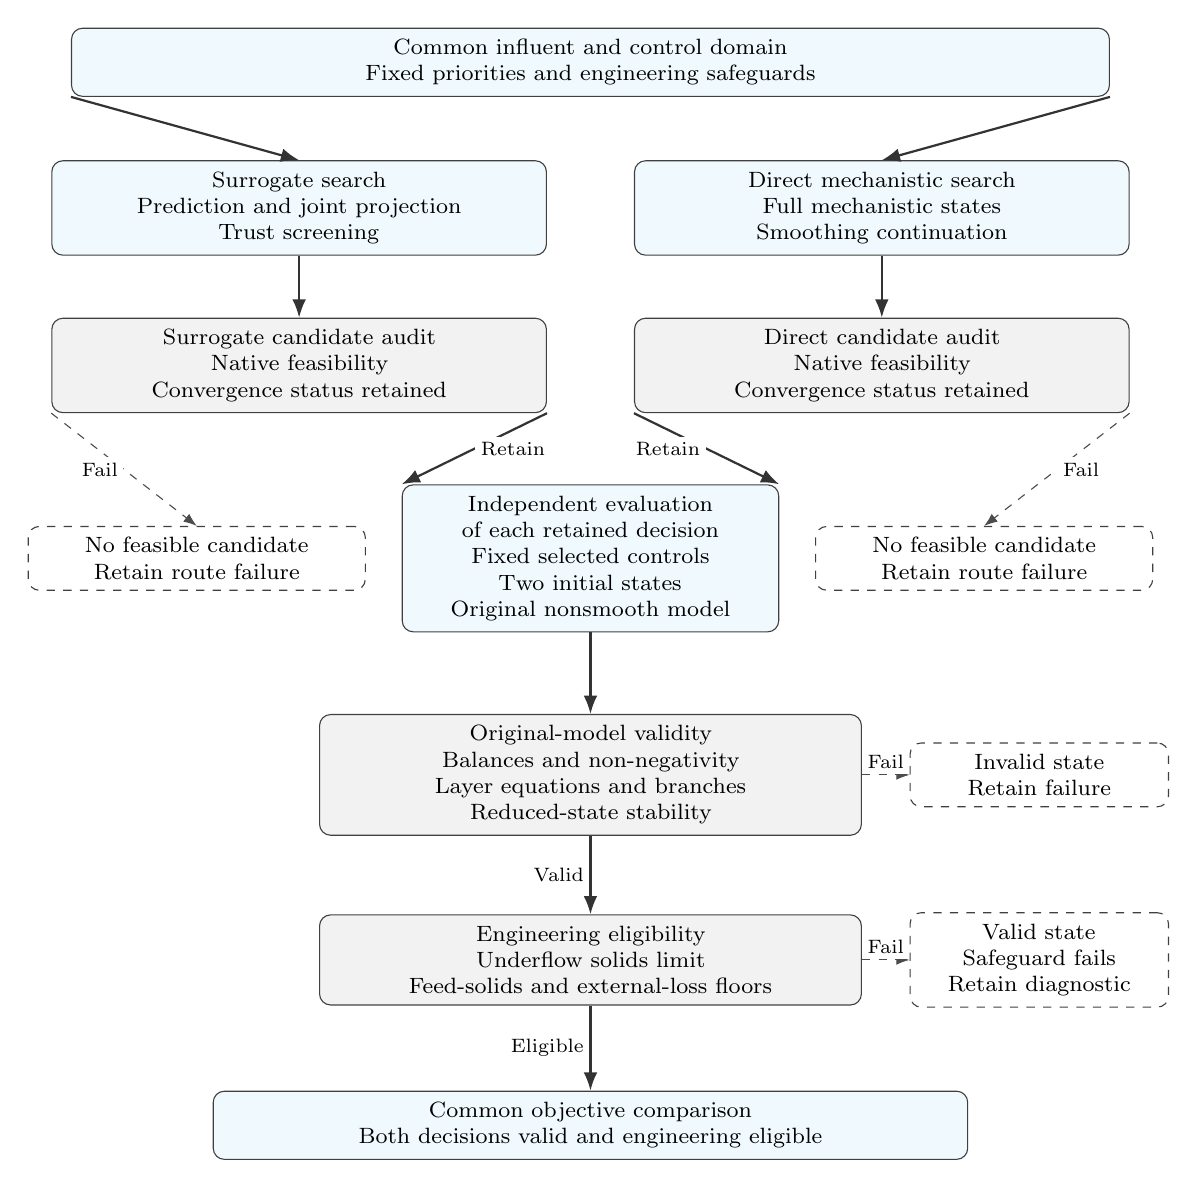
\begin{tikzpicture}[>=Latex,
block/.style={draw=black!75,rounded corners,fill=cyan!6,align=center,font=\footnotesize,inner sep=4pt},
audit/.style={block,fill=black!5},
failure/.style={block,dashed,fill=white},
flow/.style={->,thick,draw=black!80},
failflow/.style={->,dashed,draw=black!70},
lab/.style={font=\scriptsize,fill=white,inner sep=2pt}]
\node[block,text width=12.9cm] (common) at (0,0)
{Common influent and control domain\\Fixed priorities and engineering safeguards};
\node[block,text width=6.0cm] (surrogate) at (-3.7,-1.85)
{Surrogate search\\Prediction and joint projection\\Trust screening};
\node[block,text width=6.0cm] (direct) at (3.7,-1.85)
{Direct mechanistic search\\Full mechanistic states\\Smoothing continuation};
\node[audit,text width=6.0cm] (snative) at (-3.7,-3.85)
{Surrogate candidate audit\\Native feasibility\\Convergence status retained};
\node[audit,text width=6.0cm] (mnative) at (3.7,-3.85)
{Direct candidate audit\\Native feasibility\\Convergence status retained};
\node[failure,text width=4.0cm] (sfail) at (-5.0,-6.3)
{No feasible candidate\\Retain route failure};
\node[failure,text width=4.0cm] (mfail) at (5.0,-6.3)
{No feasible candidate\\Retain route failure};
\node[block,text width=4.5cm] (evaluate) at (0,-6.3)
{Independent evaluation\\of each retained decision\\Fixed selected controls\\Two initial states\\Original nonsmooth model};
\node[audit,text width=6.6cm] (valid) at (0,-9.05)
{Original-model validity\\Balances and non-negativity\\Layer equations and branches\\Reduced-state stability};
\node[failure,text width=3.0cm] (invalid) at (5.7,-9.05)
{Invalid state\\Retain failure};
\node[audit,text width=6.6cm] (engineering) at (0,-11.4)
{Engineering eligibility\\Underflow solids limit\\Feed-solids and external-loss floors};
\node[failure,text width=3.0cm] (engfail) at (5.7,-11.4)
{Valid state\\Safeguard fails\\Retain diagnostic};
\node[block,text width=9.3cm] (comparison) at (0,-13.5)
{Common objective comparison\\Both decisions valid and engineering eligible};
\draw[flow] (common.south west)--(surrogate.north);
\draw[flow] (common.south east)--(direct.north);
\draw[flow] (surrogate)--(snative);
\draw[flow] (direct)--(mnative);
\draw[flow] (snative.south east)--(evaluate.north west) node[midway,right,lab] {Retain};
\draw[flow] (mnative.south west)--(evaluate.north east) node[midway,left,lab] {Retain};
\draw[failflow] (snative.south west)--(sfail.north) node[midway,left,lab] {Fail};
\draw[failflow] (mnative.south east)--(mfail.north) node[midway,right,lab] {Fail};
\draw[flow] (evaluate)--(valid);
\draw[flow] (valid)--(engineering) node[midway,left,lab] {Valid};
\draw[failflow] (valid)--(invalid) node[midway,above,lab] {Fail};
\draw[flow] (engineering)--(comparison) node[midway,left,lab] {Eligible};
\draw[failflow] (engineering)--(engfail) node[midway,above,lab] {Fail};
\end{tikzpicture}
\caption{Conceptual paired-search and verification workflow. Each retained control vector receives its own independent original-model evaluation. The surrogate and smooth-direct native responses do not supply the reference treatment outcome. Original-model validity and engineering eligibility are distinct checks. Only eligible pairs enter the common-objective comparison, while failed or qualified cases remain in the accounting.}
\label{fig:plant_route_verification}
\end{figure}

The independent evaluation stage supplies treatment outcomes at the selected controls without feeding information back into either fitted search model. A mechanistically valid response may still violate a retained engineering safeguard and remain useful as a diagnostic. Separating these outcomes prevents numerical convergence, physical validity, and decision eligibility from being treated as the same property.

\subsubsection{Evaluation at fixed selected controls}

Every available selected decision is reevaluated with its controls and influent held fixed. Both prescribed initial states are solved using the original nonsmoothed reactor and ten-layer clarifier equations. The independently converged state supplies the reference treatment outcome for both routes. This role of an original-model check is consistent with the validation requirements discussed by \citet{BhosekarIerapetritou2018}.

Exact evaluation uses the physical checks in Table~\ref{tab:plant_generation_settings}. Agreement between the two starts is tested under both the generation scales and fixed development-derived state scales. The fixed scales are coordinatewise development-set median absolute deviations with a floor of one. A valid evaluation must pass mass conservation, non-negativity, layer residuals, the operating domain, the endpoint envelope, and the reduced-state local stability test.

Branch tuples must agree unless one evaluation start lies inside a prescribed ambiguity band. These bands cover the clarifier receiver threshold, zero storage capacity, zero settling offset, zero or maximum settling velocity, and equality of adjacent gravitational fluxes. An ambiguity flag qualifies the state-level branch comparison; it does not automatically prove that every differing branch is physically equivalent. State agreement and all other audits must still pass. Smooth stationarity or smooth-reference equivalence near such a branch boundary therefore remains explicitly qualified.

This verification is particularly important when a selected prediction lies close to a treatment requirement. The aeration-scheduling framework of \citet{Ren2026} similarly emphasizes influent disturbances and effluent ammonium safeguards. The relevant engineering question is the value of the particular effluent quantity at the selected controls, not only the model's average error elsewhere.

\subsubsection{Native and common-reference objectives}

Let route $S$ denote the connected surrogate and route $M$ the direct smooth mechanistic search. Their native responses are $\chi_{{\rm nat},S}=\widehat\chi$ and $\chi_{{\rm nat},M}=\chi_{{\rm sm},M}$. Their independently evaluated responses are $\chi_{{\rm ref},S}$ and $\chi_{{\rm ref},M}$. Raw and projected surrogate predictions are also evaluated, where defined, at both retained control vectors.

Normalization can alter an objective even when the physical response is identical. Consider an illustrative two-quality response whose development standard deviations are 0.5 and 2 in their native units. A scale with a floor of one gives denominators 1 and 2, whereas an unfloored scale gives 0.5 and 2. For response values 0.8 and 4,
\[
\begin{aligned}
\text{floored scale}&=(0.8/1,\,4/2)=(0.8,2),\\
\text{unfloored scale}&=(0.8/0.5,\,4/2)=(1.6,2).
\end{aligned}
\]
With equal internal quality weights, these give means 1.4 and 1.8. The difference arises entirely from the normalization. In matrix form,
\[
D_{T,S}^{\rm toy}=\begin{bmatrix}1&0\\0&2\end{bmatrix},\qquad
D_{T,M}^{\rm toy}=\begin{bmatrix}0.5&0\\0&2\end{bmatrix}.
\]
The paired comparison therefore evaluates both decisions on a common reference normalization so that a route-specific scaling convention is not mistaken for a treatment improvement.

For positive development-set quality standard deviations $\sigma_j$, the route-native normalizations are
\begin{equation}
\equationname{Route-specific water-quality objective scales}
D_{T,S}=\operatorname{diag}(\max(1,\sigma_j)),\qquad
D_{T,M}=\operatorname{diag}(\sigma_j).
\label{eq:plant_route_normalization}
\end{equation}
The unit floor is expressed in the physical unit of each quality quantity. The common reference objective uses $D_{T,M}$ for both selected decisions. The fitted standard deviations remain estimation outputs rather than theoretical constants.

A hypothetical comparison clarifies the two distinct objective differences. Suppose two native objectives are 0.90 and 0.95, so the native calculations favor the first decision by 0.05. Independent mechanistic evaluation instead gives 1.10 and 0.98, reversing the ordering. For the first route, the native-minus-reference difference is $0.90-1.10=-0.20$, indicating that the native calculation was optimistic relative to the independent evaluation. If the second route has native objective 0.95 and reference objective 0.98, its native-minus-reference difference is $-0.03$. Comparing the two independently evaluated decisions gives $1.10-0.98=0.12$, meaning that the first selected decision has the larger common-reference objective.

These two comparisons are
\begin{align}
\equationname{Difference between route-native and reference-model objectives}
\Delta J_{{\rm nat-ref},k}&=
J_{{\rm nat},k}(\vartheta_k,\chi_{{\rm nat},k})
-J_{\rm ref}(\vartheta_k,\chi_{{\rm ref},k}),\quad k\in\{S,M\},\\
\equationname{Reference-model objective difference between optimization routes}
\Delta J_{S-M}&=J_{\rm ref}(\vartheta_S,\chi_{{\rm ref},S})
-J_{\rm ref}(\vartheta_M,\chi_{{\rm ref},M}).
\label{eq:plant_objective_comparison}
\end{align}
The first quantity can reflect both response approximation and route-specific normalization. The second compares the retained decisions on one shared physical and numerical basis \citep{BhosekarIerapetritou2018,Pedrozo2025}.

Relative objective differences also depend on their denominator. If the common-reference difference is 0.12 and the direct objective is 0.98, the direct-relative percentage is approximately 12.24\%. A symmetric scaled difference using $\max(1,1.10,0.98)=1.10$ gives approximately 0.1091. The first uses one route as a reference; the second uses a symmetric magnitude scale.

Control differences require a different normalization. On an illustrative interval from 10 to 30, two selected controls 25 and 20 differ by five physical units, corresponding to normalized difference 0.25. If this is the only differing coordinate among seven controls, the RMS normalized difference is $\sqrt{0.25^2/7}\approx0.0945$, while the maximum difference remains 0.25. The RMS summarizes overall separation; the maximum keeps the largest coordinate change visible.

The normalized control differences are
\begin{equation}
\equationname{Normalized operating-control differences and their summaries}
d_j=\frac{\vartheta_{S,j}-\vartheta_{M,j}}{\vartheta_j^U-\vartheta_j^L},\qquad
d_{\rm rms}=\left(\frac17\sum_{j=1}^7d_j^2\right)^{1/2},\qquad
d_{\max}=\max_j|d_j|.
\end{equation}
These metrics distinguish similarity in the objective from similarity in the actual operating decisions.

Removal is reported on the concentration basis of the corresponding composite. If influent concentration is 200 mg L$^{-1}$ and effluent concentration is 2 mg L$^{-1}$, removal is
\[
100\frac{200-2}{200}=99\%.
\]
In general,
\begin{equation}
\equationname{Percentage removal of a reported water-quality quantity}
\mathcal R_j=100\left(1-\frac{z_{E,j}}{z_{{\rm in},j}}\right),
\end{equation}
provided the influent denominator is positive. Removal therefore compares concentrations on one reporting basis, whereas a full component inventory balance also requires flow rates and all represented outlet streams.

Predicted-to-reference removal errors are expressed in percentage points. Concentration percentage errors instead divide by the mechanistic effluent concentration. These two denominators can produce very different numerical impressions. For example, with influent 200 mg L$^{-1}$ and effluent values 2 and 4 mg L$^{-1}$, the concentration prediction error is 100\% relative to 2 mg L$^{-1}$, while the removal difference is only one percentage point. Reporting both keeps these interpretations distinct.

\subsubsection{Validity, engineering eligibility, and failures}

A paired objective comparison is reported only when both routes provide a natively feasible candidate, each candidate produces a valid exact mechanistic evaluation, and both exact responses satisfy the common retained engineering safeguards. A mechanistically valid response that violates an underflow, feed-solids, or external-loss safeguard remains diagnostically useful but does not enter the eligible paired comparison. Solids retention time and loading measures are reported for every finite mechanistic evaluation and do not create additional eligibility thresholds.

\begin{table}[htbp]
\centering\small
\caption{Distinct questions retained in failure and qualification accounting.}
\label{tab:plant_failure_classes}
\begin{tabular}{p{0.31\linewidth}p{0.55\linewidth}}
\toprule Assessment & Question answered\\\midrule
Generation acceptance & Did both original-model starts pass the required physical and numerical checks?\\
Projection feasibility & Did the fitted closure and physical constraints admit an audited joint response?\\
Native engineering feasibility & Did the search candidate satisfy its declared optimization constraints?\\
Convergence qualification & Did derivative audits or complete finite polls supply their stated evidence?\\
Exact-model validity & Did independent original-model evaluation converge to an accepted state?\\
Retained engineering feasibility & Did the exact response pass the common safeguards?\\
Paired eligibility & Were both decisions available and admissible on the common reference basis?\\
\bottomrule
\end{tabular}
\end{table}

These status fields are intentionally not collapsed into one success label. Missing or nonfinite quantities, undefined feature scales, failed factorizations, and inconsistent audits remain computational failures. A finite result that fails a scientific threshold remains available as a diagnostic state with the failed criterion identified. Generation rejection, projection infeasibility, optimization failure, and branch qualification therefore retain distinct meanings and denominators.

\subsubsection{Influent scenarios and time accounting}

Ten additional influent vectors from a separate twenty-dimensional Latin hypercube define the scenario experiment. They use the seed in Table~\ref{tab:plant_design_settings} and are excluded from fitting, trust calibration, and model tuning. Both optimization routes are attempted for the nominal influent and all ten scenarios. Every available selected decision receives independent exact evaluation, even when the other route fails. The scenario experiment therefore examines how the fixed fitted procedure behaves under specified influent variation.

Optimization time is defined as the duration of the route's initial search. For Extended ICSOR, this interval includes regression evaluation, joint projection, and any value-only fallback used within the initial search. For Smooth NLP, it includes the initial three-stage smoothing sequence. Development sampling, model fitting, convergence certification, conditional recovery, and independent exact evaluation are excluded. Failed initial attempts remain in the timing account. Scenario summaries use S1--S10 and keep the nominal case separate. Both routes use the same processor allocation and thread count.

Timing is reported together with search workload. Recorded quantities include evaluated points, iterations, projection retries, fallback use, completed smoothing stages, recovery status, and convergence qualification. The benchmarking concerns of \citet{Bliek2023} motivate retaining these workload indicators alongside elapsed time and objective quality.

A complete workflow comparison would additionally include development, certification, recovery, and exact verification. These terms matter when repeated use is considered because development effort can be amortized only if later per-decision savings are large enough. \citet{BhosekarIerapetritou2018} and \citet{Bliek2023} motivate this complete-cost perspective.

The arithmetic can be illustrated hypothetically. Suppose surrogate development requires 100 s, and each later surrogate-assisted decision requires 3 s in total for search, qualification, and verification. Suppose the comparable direct decision requires 6 s. For 20 decisions, total times are $100+20(3)=160$ s and $20(6)=120$ s. For 50 decisions, they are 250 and 300 s. The development effort is therefore recovered only after sufficiently many repeated decisions.

More generally, let $n_{dec}$ be the number of later decisions, $T_{dev}$ the development cost, and $T_S$ and $T_M$ the complete per-decision costs. Surrogate use is faster in total when
\[
\begin{aligned}
T_{dev}+n_{dec}T_S&<n_{dec}T_M,\\
T_{dev}&<n_{dec}(T_M-T_S),\\
n_{dec}&>\frac{T_{dev}}{T_M-T_S}\qquad\text{when }T_M>T_S.
\end{aligned}
\]
For the illustrative values above, the threshold is $100/(6-3)=33\tfrac13$, so at least 34 complete decisions are required. If the surrogate does not reduce complete per-decision cost, positive development effort cannot be recovered through timing alone. The comparison also assumes that the resulting decisions satisfy the required quality and feasibility criteria.

The complete assessment therefore retains four distinct forms of evidence. Statistical assessment concerns approximation of accepted mechanistic states. Projection audits concern the imposed network and inventory relations. Search audits concern local numerical evidence for the declared optimization problems. Independent original-model evaluation concerns treatment performance and feasibility at the selected controls. Together, these four layers determine whether the connected surrogate is useful as an operating decision aid \citep{BhosekarIerapetritou2018,Pedrozo2025}.

\section{Results}
\label{sec:plant_results}

The operating assessment compares Extended ICSOR and Smooth NLP through independent evaluation with the original mechanistic equations. The nominal influent is denoted N, and the ten additional influent cases are denoted S1--S10. Prediction accuracy, physical compliance, decision quality, and optimization time are reported separately so that improvement in one dimension is not treated as evidence of improvement in another.

\subsection{Accepted development and holdout states}

The development design retained 7{,}386 of 8{,}000 attempted mechanistic states, while the holdout design retained 1{,}845 of 2{,}000. Their acceptance fractions were 92.33\% and 92.25\%, respectively. Table~\ref{tab:plant_sample_results} gives the corresponding rejection counts. Rejected candidates were not replaced, so the retained samples reflect the realized acceptance behavior of the predefined designs. These accepted states supplied the fitting and holdout assessments.

\begin{table}[htbp]
\centering\small
\caption{Realized mechanistic samples for the connected-plant assessment. The separate development and holdout designs retained accepted states without replacing rejected candidates.}
\label{tab:plant_sample_results}
\begin{tabular}{lrrrr}
\toprule
Design & Attempted & Accepted & Rejected & Accepted (\%)\\
\midrule
Development & 8000 & 7386 & 614 & 92.33\\
Holdout & 2000 & 1845 & 155 & 92.25\\
\bottomrule
\end{tabular}
\end{table}

The raw-response model selected a ridge penalty of 0.1. Its mean grouped cross-validation normalized root error was 0.659 on the complete joint response using fitting-defined response scales. This development score and the holdout composite scores reported below use different denominators and should therefore be interpreted within their own assessment roles.

\subsection{Aggregate and local holdout accuracy}

Joint projection improved the aggregate holdout prediction. The pooled nRMSE decreased from 0.04690 for the raw response to 0.04306 after projection, corresponding to an 8.19\% reduction before rounding. The nMAE decreased from 0.03044 to 0.02568, a 15.65\% reduction, while mean location-level $R^2$ increased from 0.925 to 0.938. Figure~\ref{fig:plant_holdout_overview_results} shows that this improvement was not confined to the aggregate score: all eight treatment-location summaries and all four composite summaries had lower nRMSE after projection.

\begin{figure}[htbp]
\centering
\includegraphics[width=\textwidth,height=0.72\textheight,keepaspectratio]{compile/optimization/results/figures/q01_holdout_accuracy_overview.png}
\caption{Raw and projected composite accuracy on 1845 holdout plant states. Rows show aggregate, location, and composite summaries. Columns show nRMSE, nMAE, and mean location-level $R^2$. Errors are normalized by the mechanistic holdout range of each location and composite. The $R^2$ summaries average coordinate-specific scores rather than pooling locations into one score.}
\label{fig:plant_holdout_overview_results}
\end{figure}

The composite-level changes were also consistent with this general improvement. COD nRMSE decreased from 0.04741 to 0.04586, TN from 0.03724 to 0.03454, TP from 0.04170 to 0.03349, and TSS from 0.05852 to 0.05476. TP showed the largest relative improvement among the four composites, whereas TSS retained the largest projected error. Because these values use location-specific holdout ranges, they describe relative agreement within each reported treatment quantity rather than one common physical-unit error scale.

The location-level assessment shows where the projection helped and where it did not. Of the 32 location--composite combinations, projection reduced nRMSE in 30. Figure~\ref{fig:plant_holdout_locations_results} identifies the two exceptions: COD error increased by 0.47\% in the final reactor and by 2.36\% in the overflow. By contrast, overflow TP nRMSE decreased from 0.02948 to 0.01795, a reduction of 39.10\%. The connected projection therefore produced a broad statistical benefit, but the adjustment was not uniformly beneficial for every reported quantity at every treatment location.

\begin{figure}[htbp]
\centering
\includegraphics[width=\textwidth]{compile/optimization/results/figures/q02_holdout_accuracy_by_location.png}
\caption{Holdout nRMSE by treatment location and composite. Raw and projected heatmaps share their color scale. The third panel shows percentage change relative to raw error. Negative values indicate improvement. The mixer, five reactors, overflow, and underflow are assessed separately.}
\label{fig:plant_holdout_locations_results}
\end{figure}

\subsection{Parity across the connected treatment system}

Figure~\ref{fig:plant_holdout_parity_results} provides a direct view of projected agreement across the connected plant. For each composite, the figure pools 14{,}760 location-observations while retaining the median of each treatment location. Much of the point density lies near the one-to-one line. The mean location-level $R^2$ values were 0.944 for COD, 0.963 for TN, 0.945 for TP, and 0.899 for TSS. These values summarize the eight location-specific coefficients for each composite rather than one pooled coefficient across all observations.

\begin{figure}[htbp]
\centering
\includegraphics[width=\textwidth,height=0.72\textheight,keepaspectratio]{compile/optimization/results/figures/q03_holdout_parity_all_locations.png}
\caption{Projected composite parity across eight locations and 1845 holdout states. Both concentration axes are logarithmic. Hexagon color gives the number of location-observations, and labelled markers identify each location's median. The one-to-one line indicates exact agreement. Metric annotations retain location-specific normalization and average location-level $R^2$.}
\label{fig:plant_holdout_parity_results}
\end{figure}

The overflow remained more difficult to reproduce than the reactor locations. Its projected location-average $R^2$ was 0.876, compared with reactor averages of approximately 0.947. The projected overflow TSS nRMSE was 0.07392, and TSS was underpredicted in 1{,}008 of the 1{,}845 holdout states, or 54.6\%. The remaining cases had either exact agreement or overprediction. The connected response therefore captured the broad treatment pattern well while retaining a recognizable error concentration at the discharge solids endpoint.

\subsection{Physical audits and search qualifications}

The physical audit showed a sharp distinction between the raw and projected responses. Every raw holdout response violated at least one imposed mass-conservation relation, and 1{,}765 of the 1{,}845 raw responses contained at least one negative entry. After joint projection, no mass-conservation, non-negativity, or network-inequality violations were recorded under the stated audit definitions. The projection therefore closed the declared physical-consistency gap throughout the holdout set.

The optimization searches produced a different type of evidence. Extended ICSOR retained an initially feasible candidate for the nominal influent and all ten scenarios. Smooth NLP retained candidates for the nominal influent and nine of the ten scenarios. The initial S1 direct search did not produce a validated feasible candidate, and the permitted recovery did not resolve that outcome. A separately evaluated valid direct decision for S1 is nevertheless included in the treatment and objective figures so that the paired engineering comparison remains available. It is not counted as a successful initial direct search.

Table~\ref{tab:plant_search_qualification_results} separates candidate availability from convergence qualification. Extended ICSOR received positive first-order qualification in N, S6, and S10. Seven additional surrogate decisions were qualified by the finite-poll procedure, while S4 remained unresolved. None of the retained initial Smooth NLP candidates received a positive first-order certificate. These qualification results concern numerical evidence for the corresponding search problems; the independently solved mechanistic responses provide the reference treatment outcomes used in the engineering comparison.

\begin{table}[htbp]
\centering\small
\caption{Qualification of the initial center-start searches. Each route was attempted in eleven cases. Finite-poll qualification uses the specified directions and radii. The separately evaluated S1 direct decision appears in the paired figures but does not alter these initial-search counts.}
\label{tab:plant_search_qualification_results}
\begin{tabular}{p{7.0cm}rr}
\toprule
Outcome & Extended ICSOR & Smooth NLP\\
\midrule
Initial searches & 11 & 11\\
Retained feasible initial candidates & 11 & 10\\
First-order qualification & 3 & 0\\
Additional finite-poll qualification & 7 & 0\\
Retained candidates with unresolved qualification & 1 & 10\\
Cases without a retained initial candidate & 0 & 1\\
\bottomrule
\end{tabular}
\end{table}

\subsection{Prediction fidelity at selected controls}

Average holdout performance does not determine the error at the specific controls selected by an optimizer. Figure~\ref{fig:plant_selected_parity_results} therefore compares Extended ICSOR predictions directly with independent mechanistic evaluations at the surrogate-selected controls. Across the 44 case--composite comparisons, the median absolute concentration error was 12.75\% of the mechanistic effluent concentration and the mean was 18.43\%. Median and mean absolute removal errors were 3.26 and 5.23 percentage points. These summaries use a different input distribution and different denominators from the holdout metrics.

Several cases illustrate the practical meaning of the discrepancies. In S6, Extended ICSOR predicted COD of 151.10 mg L$^{-1}$, whereas the mechanistic evaluation gave 99.21 mg L$^{-1}$. In S10, the corresponding values were 232.23 and 167.78 mg L$^{-1}$. The surrogate therefore underestimated COD removal by 8.51 and 10.44 percentage points in these two cases. These errors were conservative with respect to treatment performance because the surrogate predicted worse COD removal than the mechanistic model produced.

The S4 nutrient predictions had the opposite implication. Extended ICSOR predicted TN of 2.67 mg L$^{-1}$, while the independent mechanistic value was 7.47 mg L$^{-1}$. It predicted TP of 2.08 mg L$^{-1}$ against a mechanistic value of 4.68 mg L$^{-1}$. TN and TP removals were consequently overstated by 16.97 and 27.33 percentage points. These discrepancies remained after physical projection and trust screening, showing that a prediction can satisfy the declared network constraints while still being inaccurate in an engineering quantity important to the decision.

Overflow TSS showed a different pattern. The surrogate overpredicted TSS in ten of the eleven selected decisions. Predicted values ranged from 5.53 to 8.05 mg L$^{-1}$, while mechanistic values ranged from 5.28 to 6.41 mg L$^{-1}$. In S1, the predicted and reference values were 7.78 and 5.77 mg L$^{-1}$, yet the corresponding removal values differed by only 0.61 percentage points. A modest removal error can therefore coexist with a substantial relative error in the low effluent concentration itself.

\begin{figure}[htbp]
\centering
\includegraphics[width=\textwidth]{compile/optimization/results/figures/q04_effluent_and_removal_parity.png}
\caption{Extended ICSOR predictions at selected controls compared with independent original-model evaluation. The upper row shows effluent concentration parity in mg L$^{-1}$. The lower row shows removal parity in percent. Columns correspond to COD, TN, TP, and TSS. Teal identifies concentrations and orange identifies removals. Labels identify N and S1--S10. Dashed lines indicate exact agreement.}
\label{fig:plant_selected_parity_results}
\end{figure}

\subsection{Treatment outcomes and operating choices}

Figure~\ref{fig:plant_controls_results} compares the two optimization routes after both selected decisions are evaluated with the original mechanistic model. Smooth NLP produced lower COD, TN, and TP in the nominal case and in nine of the ten scenarios. For the nominal influent, COD was 151.26 mg L$^{-1}$ at the Extended ICSOR decision and 57.60 mg L$^{-1}$ at the Smooth NLP decision. In S9, the corresponding values were 203.24 and 19.08 mg L$^{-1}$. TSS did not follow the same ordering consistently: Smooth NLP produced lower TSS in six of the eleven paired comparisons.

The selected HRT values show that the two routes also differed in their capacity choices. Extended ICSOR selected the 6-h lower bound in N, S6, S7, S9, and S10. Smooth NLP selected the 36-h upper bound in S5 and S10 within numerical tolerance. Because fresh flow was fixed, these HRT choices changed total biological reactor volume. The optimization therefore compared different combinations of installed biological capacity and operating controls.

Aeration and recycle patterns reveal additional structure. Both routes selected the upper aeration bound in reactor 3 for every case within numerical tolerance, and aeration in reactors 4 and 5 frequently reached the upper bound as well. Both routes selected the return-sludge lower bound of 0.25. Smooth NLP selected internal recycle $r_I=4.00$ in S2 and S10 and 3.44 in S9; in its other cases, the selected ratio was effectively zero. Extended ICSOR selected internal recycle values between zero and 0.804.

S2 illustrates why nominal HRT and residence time per passage must be distinguished. Smooth NLP selected $H=31.40$ h with $r_I=4.00$ and $r_R=0.25$. The resulting reactor-train flow ratio was 5.25, so the actual residence time per passage through the train was only about 5.98 h. High recycle therefore reduced the time associated with each passage despite the large nominal fresh-flow HRT.

Wasting frequently reached its upper bound, but the corresponding resource contribution still depended on the selected underflow solids concentration through $wX_U$. Neither the wasting ratio nor an aeration setting alone is sufficient to describe the resulting material removal or resource proxy.

\begin{figure}[htbp]
\centering
\includegraphics[width=\textwidth,height=0.76\textheight,keepaspectratio]{compile/optimization/results/figures/q05_effluent_and_operating_values.png}
\caption{Mechanistic effluent outcomes and selected controls for both optimization routes. The top row shows COD, TN, TP, and TSS in mg L$^{-1}$. The remaining panels show HRT, aeration in reactors 3--5, internal recycle, return sludge, and wasting. The unused panel is omitted. N and S1--S10 appear in every comparison. The constant aeration and return-sludge panels use plain zero-to-one axes.}
\label{fig:plant_controls_results}
\end{figure}

\subsection{Mechanistic treatment-train profiles}

Figure~\ref{fig:plant_profile_results} traces the original-model concentrations through the plant at each route's selected controls. All four reported composites increased from fresh influent to the mixer in all eleven cases for both routes. This increase reflects the material returned by the recycle streams rather than an external source of pollution \citep{Alex2008}.

The subsequent changes through the biological reactors and the clarifier have different physical meanings. Changes across the reactors reflect the combined effects of biological conversion, hydraulic transport, and solids inventory. The concentration decrease across the clarifier reflects separation of particulate material under the nonreactive clarifier assumption. A reported total may also remain nearly constant while its internal species are redistributed. For example, one nitrogen form may be converted to another without producing a large change in TN \citep{Henze2006,JeppssonDiehl1996}.

The pronounced TSS decrease from reactor 5 to the final effluent shows the role of secondary clarification in treated-water quality. Interpreting the plant response therefore benefits from retaining the individual species, outlet solids flows, and reactor and clarifier inventories in addition to the four reported composites. These quantities connect the observed profiles to nitrification, denitrification, phosphorus uptake, separation, and solids age \citep{Henze2008,Wentzel1992}.

\begin{figure}[htbp]
\centering
\includegraphics[width=\textwidth,height=0.77\textheight,keepaspectratio]{compile/optimization/results/figures/q06_treatment_train_profiles.png}
\caption{Mechanistic concentration profiles at controls selected by Extended ICSOR and Smooth NLP. Rows show COD, TN, TP, and TSS from fresh influent through the mixer and reactors 1--5 to clarifier effluent. Each composite has identical logarithmic concentration limits for both routes. Colors identify N and S1--S10. Underflow is not placed in the main liquid-treatment path.}
\label{fig:plant_profile_results}
\end{figure}

\subsection{Quality and resource trade-offs}

Smooth NLP produced the lower common-reference objective in the nominal case and in all ten scenarios. Figure~\ref{fig:plant_objective_results} separates the total objective into normalized treatment quality and weighted resource contributions so that the reason for each preference remains visible. For the nominal influent, the objectives were 0.8647 for Extended ICSOR and 0.7862 for Smooth NLP, making the surrogate-selected value 9.99\% higher relative to the direct value. S5 had the largest absolute difference, with values 1.0101 and 0.7022. S8 had the smallest, with values 0.9279 and 0.9234.

The lower Smooth NLP objectives did not always arise from the same trade-off. Smooth NLP had lower normalized quality cost in ten of the eleven cases, but its weighted resource contribution was higher in every case except S8. In S10, normalized quality cost decreased from 1.4748 to 0.3699, while weighted resource contribution increased from 0.0557 to 0.4191. The resulting total objective decreased from 0.7931 to 0.6040. The direct decision therefore accepted substantially greater capacity and resource contribution to obtain much better weighted treatment performance.

S8 showed the opposite pattern. Its normalized quality cost increased from 1.5856 to 1.6110, and all four evaluated effluent composites were slightly higher under the Smooth NLP decision. The weighted resource contribution, however, decreased from 0.1351 to 0.1179. That resource reduction was sufficient to lower the total objective from 0.9279 to 0.9234. The objective therefore preferred the direct decision even though its effluent concentrations were slightly worse.

The development quality scales were 106.61, 13.07, 7.11, and 17.38 mg L$^{-1}$ for COD, TN, TP, and TSS. Because all four exceeded one, the route-specific normalization matrices in Equation~\eqref{eq:plant_route_normalization} were identical in this experiment. The objective differences were therefore not caused by different route-specific quality scaling.

The dependence of the aeration proxy on reactor volume also influenced the trade-offs. When $H=6$ h and all three aeration settings are at one, Equation~\eqref{eq:plant_aeration_proxy_example} gives $j_A=1/6$. Several surrogate-selected decisions combined maximum aeration settings with minimum HRT and therefore incurred relatively small normalized aeration-capacity contributions. The objective measures the declared capacity and resource proxies rather than the dimensionless aeration controls alone.

\begin{figure}[htbp]
\centering
\includegraphics[width=\textwidth]{compile/optimization/results/figures/q07_objective_quality_economic.png}
\caption{Common-reference total objective, normalized quality cost, and weighted resource contributions. Both routes are evaluated with the original mechanistic model and common quality scales. Resource stacks show HRT, aeration, internal recycle, return sludge, and wasting. Solid bars identify Extended ICSOR, and hatched bars identify Smooth NLP. The quality panel shows $j_Q$, whose contribution to the total objective is $0.50j_Q$.}
\label{fig:plant_objective_results}
\end{figure}

\subsection{Optimization time}

Extended ICSOR completed the recorded initial search more quickly for the nominal influent and for every scenario. Figure~\ref{fig:plant_time_results} shows all eleven comparisons. Across S1--S10, Extended ICSOR times ranged from 0.758 to 2.702 s, whereas Smooth NLP times ranged from 3.932 to 8.253 s. Their scenario means were 1.726 and 5.236 s, respectively, giving a ratio of approximately 3.03. The nominal times were 0.985 and 5.062 s.

The direct-to-surrogate time ratio varied by scenario from 1.90 to 7.99, with the largest ratio in S10. The timing definition includes failed initial search attempts, including the failed S1 direct attempt. Whether a feasible candidate was retained is therefore reported separately in Table~\ref{tab:plant_search_qualification_results} rather than inferred from timing.

These times cover only the initial optimization intervals defined in the methodology. They exclude development sampling, fitting, convergence certification, conditional recovery, and independent mechanistic evaluation. Extended ICSOR therefore demonstrated a shorter initial search interval, but the paired engineering assessment simultaneously showed that its selected decisions had higher mechanistic objectives.

\begin{figure}[htbp]
\centering
\includegraphics[width=\textwidth]{compile/optimization/results/figures/q08_optimization_time.png}
\caption{Recorded optimization time for N and S1--S10 on a logarithmic seconds axis. The interval includes the initial surrogate search with projection and fallback or the initial direct smoothing sequence. It excludes generation, fitting, certification, conditional recovery, and independent mechanistic evaluation. Initial failed attempts remain in the timing account. Scenario mean times use S1--S10 only.}
\label{fig:plant_time_results}
\end{figure}

\section{Discussion}
\label{sec:plant_discussion}

\subsection{Connected enforcement and its statistical benefit}

The connected surrogate was designed to predict the plant as one material system rather than as a collection of independent unit outputs. Its response retained the mixer, five biological reactors, clarifier overflow and underflow, and stored solids. Joint projection then linked these quantities through the declared mixer, reactor-inventory, clarifier, separation, and storage relations. The holdout results show that this physical reconciliation was accompanied by a broad statistical benefit. Aggregate nRMSE and nMAE both decreased, all eight location summaries improved, all four composite summaries improved, and 30 of the 32 individual location--composite errors decreased.

This result is important because projection was not introduced merely as a numerical feasibility repair. The connected constraints couple locations that are physically related, so correcting one part of the response redistributes information across the treatment system. In this case, the redistribution generally moved the predictions closer to the mechanistic holdout states. The especially large reduction in overflow TP error illustrates how a network-level correction can improve a reported quantity at a downstream location even though the projection acts on the complete component response.

The improvement was nevertheless not uniform. COD error increased slightly in the final reactor and overflow, and the overflow remained the least accurate treatment location overall. The separate logarithmic model supplied a positive overflow-solids endpoint, while the joint projection reconciled that endpoint with component balances, soluble continuity, particulate densification, and inventory limits. The resulting response therefore reflected both physical equalities and an empirical closure. Equations~\eqref{eq:plant_projection_error_exact} and \eqref{eq:plant_projection_error_general} explain why error reduction depends on the projection metric and on whether the mechanistic reference lies in the complete projection set. The two local COD increases are consistent with that limitation: enforcing network consistency can improve the response in aggregate while worsening an individual reported coordinate.

The practical implication is that physical consistency and statistical accuracy should be assessed together but not conflated. The projection succeeded completely in its declared physical role, while its statistical effect was broad but not universal. This distinction is consistent with the projection analyses of \citet{SturmSilva2024} and \citet{KircherVotsmeier2025}. For connected treatment models, the relevant question is therefore not simply whether projection enforces the constraints, but also how the resulting adjustment redistributes predictive error across the locations and quantities that matter for engineering use.

\subsection{Holdout accuracy and selected-decision fidelity}

The holdout assessment showed that Extended ICSOR approximated the connected plant well over the sampled domain, but the selected-control assessment exposed a second and more demanding question. Optimization does not sample the domain uniformly. It concentrates evaluations around controls that appear favorable under the surrogate objective. Prediction error at those selected controls can therefore matter more to the final decision than average error over the broader holdout design \citep{BhosekarIerapetritou2018,Pedrozo2025}.

S4 illustrates this distinction clearly. The projected surrogate predicted TP of 2.08 mg L$^{-1}$, whereas independent mechanistic evaluation at the same controls gave 4.68 mg L$^{-1}$. TN was similarly underestimated, at 2.67 versus 7.47 mg L$^{-1}$. If, for illustration, a treatment requirement were 3 mg L$^{-1}$ for TP, the surrogate and mechanistic responses would place the same operating decision on opposite sides of the requirement. The engineering consequence is therefore not captured by the relatively favorable average holdout statistics.

The selected-control discrepancies also show why physical projection and trust screening cannot be treated as substitutes for mechanistic verification. Projection ensured consistency with the declared plant balances and bounds, while the trust diagnostics restricted search to regions of specified data support, correction size, split consistency, and reactor residual. Neither step guarantees that the surrogate reproduces the nonlinear biological and settling equations closely enough at every optimizer-selected point. A physically admissible, trusted response can still be quantitatively wrong in a nutrient concentration that governs the operating decision.

Independent evaluation closes this gap by calculating treatment outcomes from the original biological kinetics and nonlinear clarifier model at the selected controls. In this workflow, the surrogate is used to generate and screen candidate decisions, while the mechanistic model remains the reference used to judge them. The approximation-management work of \citet{Hameed2026} and the treatment-safeguard setting of \citet{Ren2026} support this separation between rapid candidate selection and reference evaluation. The results therefore support a verified decision workflow rather than unrestricted substitution of the mechanistic plant model.

\subsection{Decision quality under declared priorities}

The common-reference objective comparison gives the clearest assessment of the operating decisions themselves. Smooth NLP produced a lower mechanistic objective in the nominal case and in all ten influent scenarios. Extended ICSOR, by contrast, consistently completed the recorded initial search more quickly. The two routes therefore exhibited a trade-off between initial search computation and the quality of the retained local decisions under the declared priorities.

The objective decomposition shows that this difference cannot be summarized as ``better treatment'' versus ``lower resource use'' in one universal direction. In S10, Smooth NLP accepted a much larger capacity and resource contribution to obtain a much lower quality cost, and the treatment gain dominated the total objective. In S8, the direct route instead accepted slightly higher effluent concentrations but reduced the weighted resource contribution enough to achieve a lower total objective. Both outcomes are internally consistent with the same declared weights. The objective prefers different treatment-resource combinations because the relative contributions differ by scenario \citep{PadronPaez2020,Aboagye2021}.

This decomposition is especially important because HRT is a free decision in the present case. At fixed influent flow, increasing HRT increases biological reactor volume. Aeration cost also depends on that selected volume through the transfer-capacity proxy. The direct and surrogate routes therefore differed not only in aeration, recycle, and wasting, but also in the treatment capacity they selected. Frequent 6-h surrogate solutions favored smaller reactor volume and correspondingly smaller aeration-capacity contributions, whereas several direct solutions accepted much larger HRT to improve effluent quality.

The results should therefore be interpreted as local decisions under the specific capacity and resource priorities defined for the case study. An installed treatment plant would impose fixed reactor volumes and equipment capacities, changing the decision problem substantially. The component-resolved analysis of \citet{Zhang2026} and the energy treatment of \citet{Miederer2025} support explicit accounting of hydraulic capacity, oxygen-transfer capacity, and resource demand when interpreting such operating trade-offs.

\subsection{Computational performance and operating assessment}

The shorter Extended ICSOR search times are consistent with the mathematical structure of the two routes. The surrogate search varies only seven operating controls and obtains plant responses from second-order regression followed by a convex joint projection. Smooth NLP optimizes the controls together with reactor and clarifier states and must satisfy the smoothed mechanistic equations through a continuation sequence. The surrogate therefore performs a less expensive response calculation during the initial search.

That computational advantage is useful for repeated exploration. A fitted surrogate can evaluate many alternative aeration, recycle, wasting, and capacity combinations quickly, which is valuable when the objective is to screen candidate regions or compare responses across several influent conditions. The measured scenario mean search time was approximately three times shorter for Extended ICSOR than for Smooth NLP under the stated timing definition.

Search time, however, is only one part of the workflow. Development sampling, surrogate fitting, lower-problem projection audits, convergence qualification, conditional recovery, and independent mechanistic verification all add computational work. These terms were intentionally excluded from the reported initial-search interval and therefore cannot be inferred from Figure~\ref{fig:plant_time_results}. The complete value of the surrogate depends on whether the development cost can be amortized across repeated decisions and whether the resulting mechanistically verified decisions remain acceptable. This broader accounting follows the benchmarking principles discussed by \citet{Bliek2023}.

The convergence evidence also remains separate from decision quality. First-order qualification and finite polling assessed local numerical behavior of the surrogate optimization problem, while the direct route retained unresolved qualification in its center-start solutions. These statuses do not determine which operating decision is better. The original-model evaluation supplies that comparison. Conversely, a favorable mechanistic objective does not retroactively establish that a search was globally optimal or numerically certified.

Taken together, the results define a practical role for the connected surrogate. Extended ICSOR provides rapid candidate generation, explicit material accounting, and a fully auditable physical correction. Its search can screen operating alternatives substantially faster than the direct route under the recorded interval. The original mechanistic model then remains necessary to establish the treatment outcome and objective at the selected controls. The resulting decision aid therefore combines rapid exploration with explicit verification rather than treating computational speed as evidence of equivalent decision quality.

\subsection{Data Availability}
\label{sec:plant_data_availability}

The simulation data and numerical results supporting this study are publicly available at \url{https://github.com/egbertoselerio1997/surrogate-optimization}.
\chapter{Conclusion and Outlook}
\label{ch:conclusion}

\section{Synthesis of the research findings}
\label{sec:assessment_observed_findings}

The central research problem of this dissertation was how rapid activated sludge predictions can be used for engineering analysis when prediction accuracy alone does not establish either a usable treatment state or a good operating decision. The work addressed this problem by connecting four capabilities: complete component prediction, physical enforcement, explicit regression, and independent assessment of selected controls. Together, these capabilities form a common component-state framework, but the results show that each still requires its own evidence. A prediction can be physically consistent yet inaccurate, an inspectable regression can have higher error than a more flexible learner, and a faster operating search can select a worse decision when that decision is evaluated with the original mechanistic model.

The adopted component state retained organic substrate, nitrogen species, phosphorus storage, biomass, and solids, from which COD, TN, TP, and TSS were subsequently obtained through the reporting map \citep{Henze2006}. This ordering allowed the same predicted state to support material accounting, treatment reporting, and operating assessment without treating a reported total as if it uniquely described the underlying component composition. The following sections synthesize the findings in relation to the four research questions in Section~\ref{sec:research_questions}. The corresponding numerical evidence is reported in Sections~\ref{sec:projection_results}, \ref{sec:icsor_results}, and \ref{sec:plant_results}.

\subsection{Complete reactor prediction and data availability}

The first research question examined how accurately different learners reproduced the complete reactor response as the amount of training data changed and as inputs moved beyond the sampled domain. The common reactor benchmark showed that the preferred learner depended on the available simulation budget rather than remaining fixed across design sizes. At 500 cases, XGBoost and LightGBM had the lowest observed raw component nRMSE values of 0.435 and 0.439. At 10,000 cases, the multilayer perceptron instead had the lowest raw and projected values of 0.150 and 0.149. Because these results were obtained from a shared component target rather than separate prediction tasks, they directly address the comparative gap identified in the study. They also show why performance at one training size is insufficient to establish a universally preferred learner \citep{VieringLoog2023,Borisov2024}.

The exterior assessment added a second dimension to this conclusion by examining the usable input range. The multilayer perceptron again had the lowest error, but its projected nRMSE increased to 0.251 under mild exterior inputs and 0.521 under severe exterior inputs. Every projected exterior state nevertheless continued to satisfy the physical checks. The deterioration in severe-domain accuracy therefore arose despite, rather than because of a failure in, physical enforcement. For practical use, this means that a prediction at an unfamiliar loading or operating condition still requires an accuracy assessment even when projection returns a physically admissible state. The benchmark therefore supports model selection within declared data and domain conditions; it does not support unrestricted extrapolation or a single learner ranking that applies everywhere.

\subsection{Physical enforcement and its consequences}

The second research question examined what projection changes when it is applied to the same raw prediction. Every raw assessment state failed the specified mass conservation tolerance, although some predictors returned only non-negative concentrations. This distinction showed that positivity alone was not sufficient to establish physical admissibility. Joint enforcement returned states that passed both requirements in all 766,350 assessed projection instances. These instances included repeated assessment across nested design sizes and therefore did not represent that many distinct simulated reactor states. The maximum invariant residuals were $2.06\times10^{-13}$ in the learning domain and $1.72\times10^{-13}$ in the exterior assessment. The results demonstrate numerical enforcement of the adopted balances and concentration bounds across different learners. They apply the existing projection of \citet{KircherVotsmeier2025} to a common activated sludge prediction task rather than introducing a new projection principle.

Physical compliance, however, did not translate into uniform statistical improvement. At the largest design size, projection improved 188 of 260 predictor--component comparisons, yet aggregate component nRMSE decreased for only five of the thirteen predictors. Across all predictors, TN and TP root errors decreased, whereas COD and TSS root errors increased. Projection therefore closed the physical-compliance gap without eliminating the approximation gap. Its effect also depended on which treatment quantities were of interest: an analysis centered on nutrients could judge the adjustment differently from one centered on organic matter, biomass, or solids. These results support separate reporting of component and composite performance and reinforce the importance of the adjustment metric discussed by \citet{SturmSilva2024}.

Projection displacement and computational cost complete this assessment by showing not only whether a prediction became physically admissible, but also how much it had to change and how much computation was required to return the checked state. Under the stated batch protocol, projection dominated the repeated prediction cost of the fastest raw linear and neural models. A rapid regression evaluation is therefore not equivalent to a rapid complete prediction. The paired assessment provides a basis for selecting a learner and enforcement procedure together while keeping statistical accuracy, physical compliance, adjustment magnitude, and complete prediction cost as distinct criteria \citep{BhosekarIerapetritou2018}.

\subsection{Interpretation of the complete regression response}

The third research question examined how an explicit regression can support interpretable activated sludge prediction while still satisfying mass conservation and non-negativity. ICSOR addressed this problem through named operating, loading, curvature, and interaction terms, followed by learned component coupling and checked projection \citep{Selerio2026}. This staged structure made it possible to trace how an input contribution propagated from the fitted regression to the component state ultimately returned for engineering use. In one fitted model, 44 of 210 unique COD influent-curvature terms exceeded their reporting threshold, while 371 of 380 shared off-diagonal coupling entries exceeded theirs. The fitted representation was therefore selective in influent curvature but dense in coupling. Its interpretive contribution lies in providing an explicit and traceable response structure, not in producing a uniformly sparse model or uniquely identified biological parameters.

The predictive evidence showed where this structure may be practically useful. At 500 cases, ICSOR had the lowest mean held-out pooled composite root error of 10.79, compared with 11.26 for XGBoost and 11.45 for LightGBM. It also had the lowest reported root-error learning-curve area of 6.33 after normalization by the design-size interval. At 10,000 cases, however, the repeated-split errors were 5.94 for ICSOR and 4.62 for the multilayer perceptron, while LightGBM achieved the best mean rank across the broader assessment. These results favor ICSOR when an explicit equation and useful performance under limited simulation data are important, while more flexible learners remain preferable when the principal objective is lower error at the largest data budget. Because accuracy scoring used checked ICSOR states and affine-aligned comparator states, these comparisons do not isolate regression structure from the output-enforcement procedure.

The physical assessment further showed why interpretation must extend beyond the raw regression. Affine projection was sufficient for 436 of the 2000 fixed-partition cases, whereas the remaining 1564 required constrained linear projection. Every final state passed both adopted physical checks. Analytical raw and affine sensitivities, together with the hypothetical active-bound example, showed that a raw regression coefficient does not necessarily represent the final local response returned to the engineer. For example, interpreting an aeration effect requires following the fitted regression through component coupling and then through whichever projection constraints are active at the operating point of interest. ICSOR therefore addresses the interpretation gap through a traceable complete calculation, while questions of coefficient stability and causal process identification remain separate \citep{Selerio2026,Shen2023}.

\subsection{Connected prediction and operating decisions}

The fourth research question extended the problem from an individual reactor to a connected activated sludge plant and asked how joint prediction and projection could support operating decisions. The plant response retained the mixer, five biological reactors, clarifier overflow, clarifier underflow, and stored solids. Joint enforcement connected shared component flows and inventories across these locations rather than checking each unit independently \citep{Alex2008,JeppssonDiehl1996}. The development and holdout designs retained 7386 and 1845 mechanistic states. On the holdout set, projection reduced aggregate nRMSE from 0.04690 to 0.04306, corresponding to an improvement of 8.19\%, and reduced aggregate nMAE by 15.65\%. It also improved 30 of the 32 location--composite nRMSE values, with increases occurring only for COD in the final reactor and overflow. These findings address the network-consistency gap and show that the complete connected procedure produced a broad, although not uniform, statistical benefit.

The operating assessment then revealed an important limitation that average holdout improvement could not resolve. In S4, Extended ICSOR predicted TN and TP concentrations of 2.67 and 2.08 mg L$^{-1}$, whereas independent mechanistic evaluation gave 7.47 and 4.68 mg L$^{-1}$. These discrepancies remained after projection and trust screening. A nutrient requirement lying between the predicted and mechanistically evaluated concentrations would therefore lead to different judgments about whether the selected setting was acceptable. This result directly addresses the decision-quality gap: treatment outcomes must be evaluated at the controls actually selected by the optimization procedure rather than inferred from average holdout performance \citep{Alexandrov1998,Pedrozo2025}.

The common-reference comparison reinforced this conclusion. Smooth NLP produced a lower objective in the nominal case and in all ten influent scenarios. In the nominal case, the objective values were 0.8647 for Extended ICSOR and 0.7862 for Smooth NLP. Extended ICSOR required shorter recorded search times, but those faster searches did not match the objective values of the direct mechanistic route. The answer to the fourth research question is therefore necessarily qualified. Joint prediction and projection can support rapid exploration while maintaining a consistent material account, but they do not remove the need for mechanistic evaluation of the resulting decisions. The comparisons concern available local decisions under the declared treatment and resource priorities; they do not establish a global optimum or universal superiority of either route.

\section{Contributions and gaps addressed}
\label{sec:assessment_conclusions}

The first contribution of the dissertation is a common complete-component reactor benchmark that addresses the lack of directly comparable evidence about learner behavior under changing data availability and input conditions. Rather than assessing only a few reported treatment quantities, the benchmark retains both small component concentrations and the composite quantities derived from them. Its contribution is therefore the defined activated sludge comparison and the evidence it provides about learner behavior, not a claim that one learner is universally preferable.

The second contribution is a paired assessment of a common physical projection across different learners. This assessment makes the distinction between physical enforcement and statistical improvement directly measurable. The projection and stoichiometric foundations themselves come from existing work \citep{SturmWexler2022,KircherVotsmeier2025}; the contribution of this dissertation lies in applying them to complete activated sludge predictions and examining compliance, error redistribution, projection displacement, and computational cost together. In doing so, the study also establishes an important interpretive limit: a physically feasible component state should not be treated as if it were automatically an accurate mechanistic response.

The third contribution is the structured regression and the analysis of its complete returned response. Named terms expose operating and loading relationships, while learned component coupling represents shared dependence among the predicted outputs. Stage-specific physical diagnostics and sensitivities then distinguish what is learned by the regression from what is imposed by projection. This addresses the gap between having visible coefficients and being able to explain the final treatment prediction. The model is therefore inspectable without requiring fitted statistical associations to be interpreted as causal kinetic parameters \citep{Selerio2026}.

The fourth contribution is a connected component-state formulation with joint projection and independent verification of the operating decisions selected from it. The formulation includes shared streams and solids inventories that cannot be represented by a reactor-only output. Independent mechanistic evaluation then connects those predicted states to the treatment and resource consequences of the selected controls. Importantly, the contribution also includes the observed limitations of the surrogate-based decisions. Demonstrating shorter search times alongside higher common-reference objectives provides useful engineering evidence precisely because it avoids assuming that computational speed alone establishes decision superiority.

Table~\ref{tab:integrated_observed_findings} summarizes these gaps, the corresponding findings, and their practical uses. The integration provides a consistent assessment logic across the dissertation, but it does not imply that the numerical scores from the three studies can be combined into a single ranking. Reactor component errors use training-based scales, the structured comparison pools native composite coordinates, and plant holdout errors use location-specific reference ranges. Their validation designs and enforcement procedures also differ. Each set of results must therefore be interpreted within its own assessment rather than treated as directly interchangeable across studies.

\begin{table}[htbp]
\centering\small
\caption{Research gaps, observed answers, and practical uses of the integrated findings.}
\label{tab:integrated_observed_findings}
\begin{tabular}{>{\raggedright\arraybackslash}p{0.24\textwidth}>{\raggedright\arraybackslash}p{0.40\textwidth}>{\raggedright\arraybackslash}p{0.26\textwidth}}
\toprule
Research gap & Observed answer & Practical use\\
\midrule
Uncertain complete-state learner performance & The leading learner changed with data budget, and exterior accuracy deteriorated despite physical compliance & Select for the available data and intended input range\\
Training does not establish physical compliance & All 766,350 projected instances passed both checks, but aggregate error improved for only five of thirteen learners at the largest size & Check balances and bounds separately from treatment accuracy\\
Visible terms do not explain the final response & ICSOR exposed operating and loading terms, while most fixed-partition cases required constrained projection & Interpret the coupled and projected response at the operating point\\
Consistent unit predictions do not establish good plant decisions & Joint prediction improved 30 of 32 local scores, but faster surrogate searches selected higher reference objectives & Verify selected controls with the original plant equations\\
\bottomrule
\end{tabular}
\end{table}

Taken together, these contributions connect process knowledge, statistical approximation, physical enforcement, interpretation, and decision evidence within one assessment framework. Reaction stoichiometry supplies the invariant relations, while unit boundaries provide the transport and inventory relations that connect the treatment system \citep{Henze2006,Alex2008}. Regression approximates the mechanistic response within the sampled conditions, and projection imposes the declared physical requirements on the returned state. Interpretation then follows the complete prediction mapping, while independent mechanistic evaluation establishes the reference treatment outcome at the selected controls. The integrated contribution of the dissertation is this defined connection among the stages and the evidence used to assess each one. It does not claim invention of activated sludge stoichiometry, general projection methods, or surrogate optimization.

\section{Practical implications}
\label{sec:assessment_practical_implications}

\subsection{Treatment and resource priorities}

The operating results illustrate how treatment gains can be considered together with the resources required to obtain them. In S10, the direct decision reduced normalized quality cost from 1.4748 to 0.3699 while increasing the weighted resource contribution from 0.0557 to 0.4191. The total objective consequently decreased from 0.7931 to 0.6040. The selected decision therefore accepted greater capacity and resource contributions in exchange for substantially better weighted treatment. S8 illustrated a different trade-off: a lower resource contribution produced a slightly lower total objective even though all four effluent composites were slightly higher. Presenting the quality and resource contributions separately makes these choices easier to interpret and relate to the treatment priorities represented by the objective \citep{PadronPaez2020,Aboagye2021}.

The selected HRT values provide a corresponding link between operating decisions and capacity planning. Because fresh flow was fixed, varying HRT changed the biological reactor volume. The direct route reached the 36-h upper bound in S5 and S10, whereas the surrogate reached the 6-h lower bound in several cases. Comparing these settings with the resulting treatment performance shows how reactor capacity enters the operating trade-off. Aeration can be interpreted alongside reactor volume because both affect oxygen-transfer capacity, while wasted-solids production can be related to the wasting flow and underflow concentration. At an installed plant, the available reactor volumes and equipment capacities would provide the physical basis for making the same type of comparison among feasible control settings \citep{Henze2008,Miederer2025}.

More generally, separating quality and resource terms provides a practical basis for constructing facility-specific operating objectives. Effluent concentrations and removal values can represent treatment targets, while electricity demand, recycle pumping, sludge handling, and related quantities can represent resource priorities. The assigned weights determine how strongly each quantity influences the preferred operating decision. Presenting the resulting contributions separately allows engineers to explain why one operating condition is preferred and to examine how that preference changes when the treatment or resource priorities change \citep{PadronPaez2020,Miederer2025}.

\subsection{A verified decision workflow}

The results support a workflow in which the surrogate is used primarily for screening and candidate selection rather than as the final authority on the operating decision. The engineer first defines the plant boundary, influent composition, available controls, and treatment targets. The fitted surrogate then generates component responses for comparing alternatives, after which joint projection reconciles the predicted streams and inventories before treatment and resource quantities are evaluated. Physical residuals and projection displacement provide additional diagnostic information that can be used to identify candidates requiring more detailed assessment.

Independent evaluation with the original reaction and settling equations then supplies the final-effluent concentrations, shared solids flows, inventories, and common-reference objective at the selected controls. These quantities place alternative candidates on the same mechanistic basis and therefore provide a consistent foundation for choosing among them. The same evaluations can also identify regions in which additional mechanistic cases would be most useful, allowing subsequent surrogate fitting to concentrate on the operating conditions most relevant to the decisions being made \citep{Alexandrov1998,Hameed2026}.

The component- and location-resolved representation also supports process diagnosis. An increase from fresh-influent to mixer concentrations reveals the material circulated through recycle, while the TSS decrease across the clarifier reflects the contribution of solids separation. Separate ammonium and oxidized-nitrogen concentrations can reveal redistribution among nitrogen forms even when the total nitrogen concentration changes little. Examining these quantities together with returned solids flows and inventories allows engineers to relate aeration, recycle, and wasting decisions to the treatment response rather than relying only on final aggregate indicators \citep{Henze2006,Alex2008,JeppssonDiehl1996}.

\subsection{Computational value}

The measured scenario mean initial-search times were 1.726 s for Extended ICSOR and 5.236 s for Smooth NLP, giving a ratio of approximately 3.03. The shorter surrogate search interval provides computational value when many operating alternatives must be explored, such as across several influent conditions or combinations of aeration, recycle, and wasting settings. In this role, the surrogate reduces the time required for broad screening even though selected candidates still require mechanistic evaluation.

The value of this workflow becomes more relevant when the fitted surrogate is used repeatedly. Model-development effort can then be distributed across many subsequent operating comparisons, while expensive mechanistic calculations are reserved for the candidates most relevant to the decision. The surrogate therefore supports broader exploration, and the mechanistic model supplies detailed verification where it matters. This division of work focuses computational effort on the operating decisions of interest rather than requiring every alternative to be evaluated with the full mechanistic model from the outset \citep{BhosekarIerapetritou2018,Bliek2023}.

\section{Directions for future research}

\subsection{Adaptive sampling around operating decisions}

A natural extension of the present work is to generate additional mechanistic cases in regions where the surrogate most strongly influences the operating decision. An initial surrogate could first screen the declared domain and identify promising control settings. Mechanistic calculations at or near those candidates could then supply additional training states, concentrating new simulations on locations associated with large nutrient discrepancies, strong projection displacements, or treatment requirements that are nearly active. Repeating the fitting and operating-assessment cycle would connect the simulation budget more directly to the decisions the surrogate is intended to support. This direction develops the reference-informed model management of \citet{Alexandrov1998} and the gray-box approximation management discussed by \citet{Hameed2026}.

A useful comparison would hold the mechanistic evaluation budget fixed while contrasting uniform sampling, error-based sampling, and decision-based sampling. The assessment should include effluent errors at the selected controls, the common-reference objective, the number of accepted decisions, and the complete computational time required to deliver them. The nutrient discrepancies observed in S4 provide a concrete case for such a study. Additional mechanistic states around those selected operating conditions could determine whether focused sampling improves TN and TP prediction specifically where those quantities influence the operating choice.

\subsection{Projection aligned with treatment priorities}

The reactor results also motivate further study of the weights used during projection and of the engineering quantities those weights emphasize. A projection that minimizes adjustment in component coordinates can redistribute error differently from one designed around reported nutrients, solids, or other treatment quantities. Future formulations could compare component scaling, composite-sensitive weighting, and weights informed by prediction uncertainty. The underlying mass conservation and non-negativity requirements should remain unchanged so that any differences in treatment accuracy can be attributed to the adjustment metric itself. The species-weighted correction of \citet{SturmSilva2024} provides a precedent for incorporating component magnitude and uncertainty into this choice.

The connected plant provides a broader setting in which to test the same idea. Projection weights could distinguish the importance of internal-state accuracy from that of final-effluent accuracy while still preserving the required unit connections. For example, nutrient-focused weighting could be assessed for its ability to improve predictions at selected controls without introducing large errors in biomass, solids inventory, or other treatment locations. Such a comparison would make the relationship between the physical adjustment and the intended engineering decision more explicit.

\subsection{Uncertainty-aware prediction and operating safeguards}

A further extension is to represent uncertainty alongside the projected point prediction. Repeated fits, model ensembles, or probabilistic component predictions could be used to describe variation in the estimated treatment response, with each sampled state projected onto the same physical set. The resulting distributions could then be evaluated against mechanistic reference concentrations, particularly for TN, TP, and overflow TSS. The conservation-aware probabilistic framework of \citet{Hansen2024} and the differentiable probabilistic projection of \citet{Utkarsh2025} provide starting points for developing such an approach.

These distributions could subsequently be incorporated into operating safeguards. For example, an operating condition might be selected only when an upper predictive bound for TP remains below a specified treatment requirement. Mechanistic and plant-based evaluations could then test how often such safeguards are actually satisfied. The effluent ammonium safeguards considered by \citet{Ren2026} illustrate how treatment requirements can be incorporated into aeration decisions. Separating uncertainty arising from surrogate fitting, influent measurements, and mechanistic parameters would further show which sources of information provide the greatest improvement in decision reliability \citep{Machado2014,Petersen2003}.

\subsection{Stable interpretation of the complete response}

Further work on interpretation can examine whether the fitted coefficient groups remain stable across repeated training samples and different operating domains. The present model already provides natural groups for operating terms, loading terms, curvature, and component coupling. Resampling can reveal which groups remain consistently important and which individual coefficients vary substantially. Comparisons based on the complete predicted response can also identify cases in which different coefficient combinations produce similar treatment behavior. This would directly address the coefficient-stability question identified by \citet{Selerio2026}.

Sensitivity analysis should likewise continue through the final projection rather than stop at the raw regression. Derivatives can be evaluated at representative operating points and checked against direct perturbations of the returned concentrations. Mapping the active constraints would show where a nutrient response changes smoothly and where a projection boundary alters its local slope. Comparing these projected sensitivities with mechanistic sensitivities would provide a stronger connection between model inspection and practical decisions involving aeration, recycle, and wasting \citep{Selerio2026,Shen2023}.

\subsection{Dynamic prediction and control}

The steady-state framework can also be extended to dynamic treatment prediction by replacing fixed component states with trajectories of component concentrations and stored solids. The corresponding governing balances would include the time derivatives of reactor and clarifier inventories \citep{Takacs1991,Alex2008}. Training data could then represent changing influent loads, aeration schedules, recycle settings, and sludge wasting, while physical enforcement would account for the material transported and transformed over each prediction interval.

Such an extension would support predictive-control studies under daily influent variation and other load disturbances. Assessment could include transient nutrient peaks, recovery time, inventory changes, oxygen demand, and the computation required at each control update. The field-tested aeration controller of \citet{Bernardelli2020} and the wastewater control review of \citet{Croll2023} provide relevant examples for developing and evaluating dynamic strategies. The connected component representation developed here provides a useful starting point because it already retains the treatment locations and inventories that influence delayed process responses.

\subsection{Plant validation, topology, and resource models}

Validation with measured plant data is a major next step. Such studies could combine influent fractionation, calibrated mechanistic parameters, concentrations measured at different treatment units, clarifier solids measurements, and recorded operating controls \citep{Petersen2003,Machado2014,Newhart2019}. A prospective assessment could fix the fitting and operating procedures before the final evaluation period is collected \citep{Kaufman2012}. Testing across seasons and loading conditions would then provide evidence about how well the component surrogate transfers from simulated steady-state responses to observed treatment behavior.

The operating objectives can also be adapted to individual facilities. An installed plant has fixed reactor volumes, aeration capacity, recycle capacity, and discharge requirements. Electricity demand, chemical consumption, sludge handling, and operating costs could therefore replace or supplement the engineering proxies used in the present study \citep{Henze2008,Miederer2025}. Multiobjective studies could present the attainable combinations of treatment performance and resource demand before a specific preference is imposed. Extensions to other reactor arrangements, attached-growth systems, and resource-recovery connections could retain the same underlying principle: define the relevant component states and boundary streams before imposing physical enforcement \citep{Henze2008,Aboagye2021,Durkin2024}.

More extensive optimization comparisons could likewise consider several initial control vectors, hybrid surrogate--mechanistic searches, and the fifteen-start basin-sensitivity design described in Chapter~\ref{ch:plant}. Recording the costs of state generation, fitting, prediction, projection, search, and verification would provide a fuller basis for determining when surrogate development becomes worthwhile for repeated decisions \citep{BhosekarIerapetritou2018,Bliek2023}. The central comparison would remain the treatment outcome and common-reference objective obtained for a given computational budget.

\section{Concluding perspective}

This dissertation shows how complete component prediction, physical enforcement, interpretation, and decision verification can be brought together within one activated sludge analysis framework. Its findings answer the research questions without allowing one capability to stand as evidence for another. Learner performance depended on the amount of available data and on the input range being considered. Projection reliably enforced the adopted physical requirements, but it did not improve every prediction error. Structured regression made the treatment response inspectable, but it did not achieve the lowest error at the largest data budget. At the plant scale, connected projection generally improved prediction, while independent mechanistic evaluation showed that the faster surrogate-based searches selected decisions with higher common-reference objectives.

The practical contribution is therefore a defined workflow for rapid exploration with explicit checks on both the predicted state and the operating decision selected from it. A surrogate can be used to screen a broad set of alternatives efficiently, while the original mechanistic model remains the reference for evaluating treatment performance at promising candidate controls. Extending this workflow to actual plant operation will require measured plant data, facility-specific constraints, and locally relevant treatment and resource priorities. Within those limits, computational efficiency has value when it helps deliver an acceptable and verifiable treatment decision, not merely when it reduces search time.

\backmatter
\bibliographystyle{bibstyles/apacite_dissertation}
\bibliography{references}

\chapter*{About the Author}
\addcontentsline{toc}{chapter}{About the Author}
\markboth{About the Author}{About the Author}

\begin{center}
\includegraphics[width=0.32\textwidth]{eselerio_photo.jpg}
\end{center}

Egberto F. Selerio Jr. obtained his Bachelor of Science degree in Industrial Engineering from the University
of San Jose-Recoletos, Philippines. He obtained his Master of Science degree in Industrial Engineering from
the University of San Carlos--Talamban, Philippines. He has published 28 journal articles in applied
operations research, data science, and environmental engineering, with an H-index of 18. He is presently a
senior data scientist at Arch, an S\&P 500 insurance company, and a student in the Doctor of Engineering
program at the University of San Carlos--Talamban, Philippines.

\cleardoublepage
\chapter*{List of Publications and Presentations}
\addcontentsline{toc}{chapter}{List of Publications and Presentations}
\markboth{List of Publications and Presentations}{List of Publications and Presentations}

\section*{Publication}

Selerio, E. F. (2026). An interpretable statistical surrogate of activated sludge systems that preserves mass
conservation and component non-negativity. \textit{Digital Chemical Engineering, 20}, Article 100329.
doi: 10.1016/j.dche.2026.100329

Selerio, E. (2026, October 5). Plant-wide optimization of activated sludge systems using a physically constrained statistical surrogate. \textit{SSRN}. doi: 10.2139/ssrn.7567818

\section*{Presentation}

Selerio, E. F. (2023, April 21--22). \textit{Mass transport, biofilm accumulation, and biotransformation in
recycling down-flow hanging sponge systems} [Poster presentation]. 4th International Conference on Sustainable
Energy Ecosystems (SEECON 2023), University of San Carlos--Talamban Campus, Cebu City, Philippines.

\end{document}
